% BSD 3-Clause License
%
% Copyright (c) 2023 Quux System and Technology. All rights reserved.
%
% Redistribution and use in source and binary forms, with or without
% modification, are permitted provided that the following conditions are met:
%
% 1. Redistributions of source code must retain the above copyright notice, this
%    list of conditions and the following disclaimer.
%
% 2. Redistributions in binary form must reproduce the above copyright notice,
%    this list of conditions and the following disclaimer in the documentation
%    and/or other materials provided with the distribution.
%
% 3. Neither the name of the copyright holder nor the names of its
%    contributors may be used to endorse or promote products derived from
%    this software without specific prior written permission.
%
% THIS SOFTWARE IS PROVIDED BY THE COPYRIGHT HOLDERS AND CONTRIBUTORS "AS IS"
% AND ANY EXPRESS OR IMPLIED WARRANTIES, INCLUDING, BUT NOT LIMITED TO, THE
% IMPLIED WARRANTIES OF MERCHANTABILITY AND FITNESS FOR A PARTICULAR PURPOSE ARE
% DISCLAIMED. IN NO EVENT SHALL THE COPYRIGHT HOLDER OR CONTRIBUTORS BE LIABLE
% FOR ANY DIRECT, INDIRECT, INCIDENTAL, SPECIAL, EXEMPLARY, OR CONSEQUENTIAL
% DAMAGES (INCLUDING, BUT NOT LIMITED TO, PROCUREMENT OF SUBSTITUTE GOODS OR
% SERVICES; LOSS OF USE, DATA, OR PROFITS; OR BUSINESS INTERRUPTION) HOWEVER
% CAUSED AND ON ANY THEORY OF LIABILITY, WHETHER IN CONTRACT, STRICT LIABILITY,
% OR TORT (INCLUDING NEGLIGENCE OR OTHERWISE) ARISING IN ANY WAY OUT OF THE USE
% OF THIS SOFTWARE, EVEN IF ADVISED OF THE POSSIBILITY OF SUCH DAMAGE.
%
\RequirePackage[l2tabu, orthodox]{nag}
\documentclass{cookbook}
\input{git-revision.tex}
\usepackage{bookmark}
	\hypersetup{
		unicode=true,
		pdfduplex={DuplexFlipLongEdge},
		pdfprintscaling={AppDefault},
		pdfpicktraybypdfsize={true},
		pdfcreator={XeLaTeX},
		pdfproducer={Quux System and Technology},
		pdftoolbar={true},
		pdftitle={四川菜谱1972重制版},
		pdfsubject={四川菜谱},
		pdfauthor={成都市饮食公司},
		pdfkeywords={川菜},
		pdflang={zh-CN},
		pdfinfo={
			GitCommitName={\gitcommitname},
			GitCommitHash={\gitcommithash},
			GitCommitterDate={\gitcommitterdate},
			PDFBuildHost={\pdfbuildhost}
		},
		hidelinks
	}
\usepackage{scalefnt}
\usepackage{pdfpages}
\usepackage{pdfoverlay}

\begin{document}
\begin{cookbook}

\pagestyle{empty}
\pagenumbering{Alph}%	Upper case letter page numbers (and reset to 1)
\bookmarksetup{startatroot}%
% Front cover
\hypertarget{front-cover}{}%
\bookmark[dest=front-cover,level=section]{封面}%
\includepdf[pages=1]{front-cover.pdf}
\clearpage
\hypertarget{inside-front-cover}{}%
\bookmark[dest=inside-front-cover,level=section]{封二}%
\null%
\cleardoublepage

\hypertarget{half-title}{}%
\bookmark[dest=half-title,level=section]{书名页}%
\enlargethispage{1\baselineskip}
% BSD 3-Clause License
%
% Copyright (c) 2023 Quux System and Technology. All rights reserved.
%
% Redistribution and use in source and binary forms, with or without
% modification, are permitted provided that the following conditions are met:
%
% 1. Redistributions of source code must retain the above copyright notice, this
%    list of conditions and the following disclaimer.
%
% 2. Redistributions in binary form must reproduce the above copyright notice,
%    this list of conditions and the following disclaimer in the documentation
%    and/or other materials provided with the distribution.
%
% 3. Neither the name of the copyright holder nor the names of its
%    contributors may be used to endorse or promote products derived from
%    this software without specific prior written permission.
%
% THIS SOFTWARE IS PROVIDED BY THE COPYRIGHT HOLDERS AND CONTRIBUTORS "AS IS"
% AND ANY EXPRESS OR IMPLIED WARRANTIES, INCLUDING, BUT NOT LIMITED TO, THE
% IMPLIED WARRANTIES OF MERCHANTABILITY AND FITNESS FOR A PARTICULAR PURPOSE ARE
% DISCLAIMED. IN NO EVENT SHALL THE COPYRIGHT HOLDER OR CONTRIBUTORS BE LIABLE
% FOR ANY DIRECT, INDIRECT, INCIDENTAL, SPECIAL, EXEMPLARY, OR CONSEQUENTIAL
% DAMAGES (INCLUDING, BUT NOT LIMITED TO, PROCUREMENT OF SUBSTITUTE GOODS OR
% SERVICES; LOSS OF USE, DATA, OR PROFITS; OR BUSINESS INTERRUPTION) HOWEVER
% CAUSED AND ON ANY THEORY OF LIABILITY, WHETHER IN CONTRACT, STRICT LIABILITY,
% OR TORT (INCLUDING NEGLIGENCE OR OTHERWISE) ARISING IN ANY WAY OUT OF THE USE
% OF THIS SOFTWARE, EVEN IF ADVISED OF THE POSSIBILITY OF SUCH DAMAGE.
%
\begingroup%
\setlength{\parindent}{0pt}%

\null%

\vfill%

\begin{center}%
{\zihao{1}\bfseries \makebox[3.666666em][s]{四川菜谱}}%
\end{center}%

\vfill%

\endgroup%

% vim: filetype=tex noautoindent nojoinspaces
% vim: fileencoding=utf-8 formatoptions+=m
% vim: textwidth=78 tabstop=4 shiftwidth=4 softtabstop=4

\cleardoublepage

\hypertarget{frontispiece}{}%
\bookmark[dest=frontispiece,level=section]{卷首插图}%
% BSD 3-Clause License
%
% Copyright (c) 2023 Quux System and Technology. All rights reserved.
%
% Redistribution and use in source and binary forms, with or without
% modification, are permitted provided that the following conditions are met:
%
% 1. Redistributions of source code must retain the above copyright notice, this
%    list of conditions and the following disclaimer.
%
% 2. Redistributions in binary form must reproduce the above copyright notice,
%    this list of conditions and the following disclaimer in the documentation
%    and/or other materials provided with the distribution.
%
% 3. Neither the name of the copyright holder nor the names of its
%    contributors may be used to endorse or promote products derived from
%    this software without specific prior written permission.
%
% THIS SOFTWARE IS PROVIDED BY THE COPYRIGHT HOLDERS AND CONTRIBUTORS "AS IS"
% AND ANY EXPRESS OR IMPLIED WARRANTIES, INCLUDING, BUT NOT LIMITED TO, THE
% IMPLIED WARRANTIES OF MERCHANTABILITY AND FITNESS FOR A PARTICULAR PURPOSE ARE
% DISCLAIMED. IN NO EVENT SHALL THE COPYRIGHT HOLDER OR CONTRIBUTORS BE LIABLE
% FOR ANY DIRECT, INDIRECT, INCIDENTAL, SPECIAL, EXEMPLARY, OR CONSEQUENTIAL
% DAMAGES (INCLUDING, BUT NOT LIMITED TO, PROCUREMENT OF SUBSTITUTE GOODS OR
% SERVICES; LOSS OF USE, DATA, OR PROFITS; OR BUSINESS INTERRUPTION) HOWEVER
% CAUSED AND ON ANY THEORY OF LIABILITY, WHETHER IN CONTRACT, STRICT LIABILITY,
% OR TORT (INCLUDING NEGLIGENCE OR OTHERWISE) ARISING IN ANY WAY OUT OF THE USE
% OF THIS SOFTWARE, EVEN IF ADVISED OF THE POSSIBILITY OF SUCH DAMAGE.
%
\pdfoverlaySetGraphicsOptions{height=147.997333mm}%
\pdfoverlaySetPDF{sagittaria-sagittifolia.pdf}%

\null%

% vim: filetype=tex noautoindent nojoinspaces
% vim: fileencoding=utf-8 formatoptions+=m
% vim: textwidth=78 tabstop=4 shiftwidth=4 softtabstop=4

\index{茨菰}%
\cleardoublepage

\hypertarget{title-page}{}%
\bookmark[dest=title-page,level=section]{标题页}%
\enlargethispage{1.75\baselineskip}
\null%
\vspace{.75\baselineskip}
\begin{center}
\begin{tabular}{r}
	{\Huge\bfseries \makebox[3.86em][s]{四川菜谱}}\\%
	{\normalsize\bfseries 1972\,\makebox[2.78em][s]{重制版}}%
\end{tabular}

\vfill

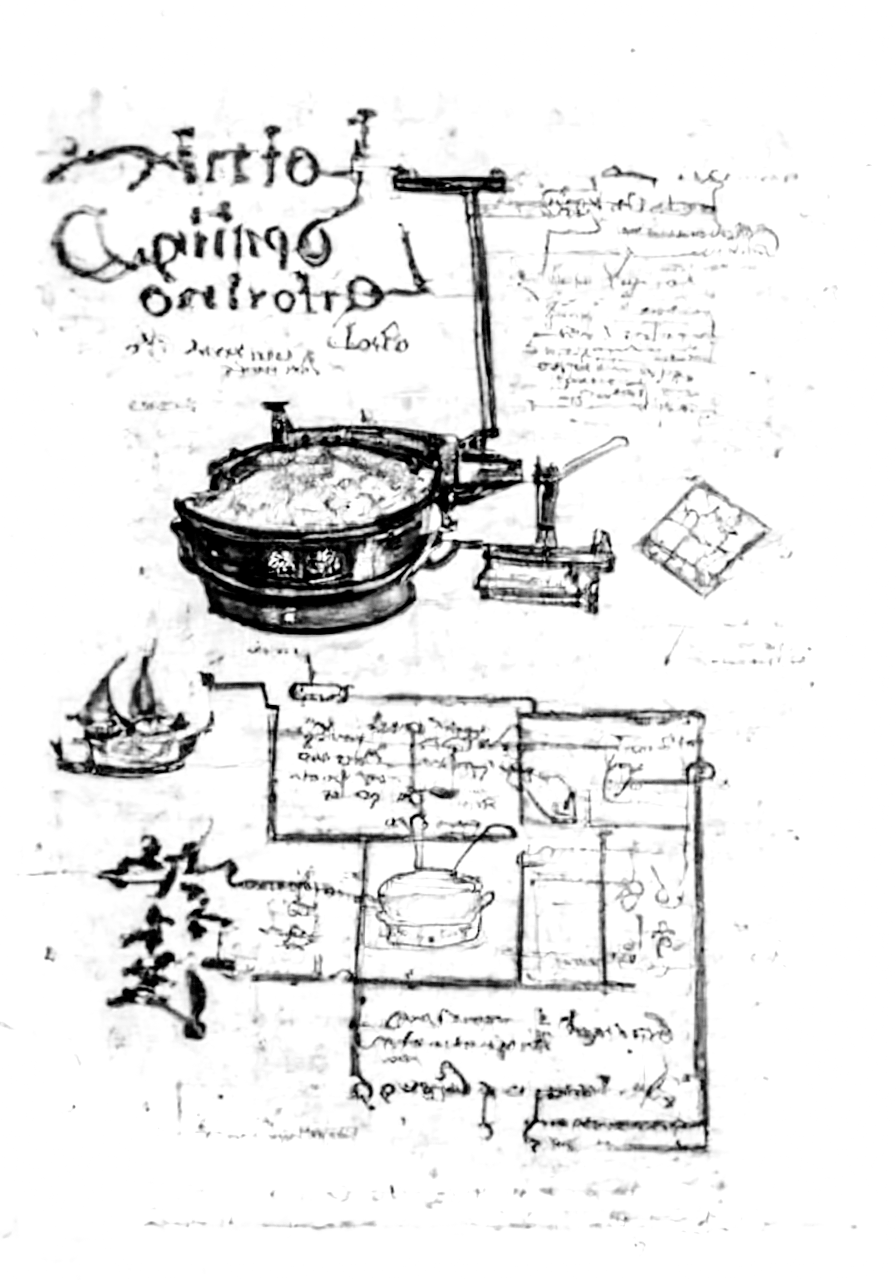
\includegraphics[height=118.070219mm]{cooking-machine.png}%

\vfill

{\footnotesize \textsc{Quux} System and Technology}
\end{center}

% vim: filetype=tex noautoindent nojoinspaces
% vim: fileencoding=utf-8 formatoptions+=m
% vim: textwidth=78 tabstop=4 shiftwidth=4 softtabstop=4

\clearpage
\hypertarget{copyright}{}%
\bookmark[dest=copyright,level=section]{版权页}%
\begingroup%
\footnotesize%
\singlespacing%
\setlength{\parindent}{0pt}%
\setlength{\parskip}{.1875\baselineskip}%
{\sffamily\bfseries Sichuan Cookbook 1972 Remake\!%
(四川菜谱\,1972\,重制版)}\\
by \textsc{Chengdu} Catering Company of \textsc{Sichuan}\!%
(四川省成都市饮食公司)

\null

Copyright {\lower.125\baselineskip\hbox{\normalsize\copyright}} 2023
\textsc{Quux} System and Technology. All rights reserved.

Redistribution and use in source and binary forms, with or without
modification, are permitted provided that the following conditions are met:

\begin{enumerate}
\item Redistributions of source code must retain the above copyright notice,
      this list of conditions and the following disclaimer.

\item Redistributions in binary form must reproduce the above copyright notice,
      this list of conditions and the following disclaimer in the documentation
      and/or other materials provided with the distribution.

\item Neither the name of the copyright holder nor the names of its
      contributors may be used to endorse or promote products derived from
      this software without specific prior written permission.
\end{enumerate}

\begingroup%
\setstretch{.9375}%
\textsc{this software is provided by the copyright holders and contributors
``as is'' and any express or implied warranties, including, but not limited to,
the implied warranties of merchantability and fitness for a particular purpose
are disclaimed. in no event shall the copyright holder or contributors be
liable for any direct, indirect, incidental, special, exemplary, or
consequential damages (including, but not limited to, procurement of
substitute goods or services; loss of use, data, or profits; or business
interruption) however caused and on any theory of liability, whether in
contract, strict liability, or tort (including negligence or otherwise)
arising in any way out of the use of this software, even if advised of the
possibility of such damage.}

\endgroup

\vfill

\setlength{\parskip}{.3125\baselineskip}%
\vspace{-2\baselineskip}
\begin{tabbing}
\hspace{9.5625em}\= \kill
\textsc{git} commit name:       \>\texttt{\gitcommitname}\\
\textsc{git} commit hash:       \>\texttt{\gitcommithash}\\
\textsc{git} committer date:    \>\texttt{\gitcommitterdate}\\
\textsc{pdf} build date:        \>\texttt{\pdfbuilddate}\\
\textsc{pdf} build host:        \>\texttt{\pdfbuildhost}
\end{tabbing}
\vspace{-1\baselineskip}

Book design and collation by \textsc{Gong}~Jie\!(龚颉)\!\!.\\
Title page illustration by Disco Diffusion v5.61 with prompt ``A detailed
automatic cooking machine blueprint by Leonardo da Vinci journal. In this
blueprint, Mapo Tofu is being cooked.''\\
This book is composed in
% XeLaTeX
\begingroup%
\rmfamily%
\footnotesize%
X\kern-.1em\lower.5ex\hbox{\scalebox{-1}[1]{E}}\kern-.15em%
L\kern-.36em\lower-.428571ex\hbox{\tiny{A}}\kern-.15em%
T\kern-.1667em\lower.5ex\hbox{E}\kern-.125emX%
\endgroup%
.

This book is designed to represent the first edition of the paperback book
\textit{Sichuan Cookbook}{\kafamily(四川菜谱)}\!\! by \textsc{Chengdu}
Catering Company of \textsc{Sichuan}\!(四川省成都市饮食公司)\!\!, which was
released in July 1972. Special care has been made to preserve the original
appearance of this book's typographical layouts,
\begin{wrapfigure}{r}{19.0625mm}%
\vspace{-1.25\baselineskip}%
\begin{flushright}%
\quad
\includegraphics[height=10mm, width=10mm]{quux-logo.pdf}%
\end{flushright}%
\vspace{-1.75\baselineskip}%
\end{wrapfigure}%
font styles, font sizes, and illustrations.

See also \url{https://github.com/neo954/sichuan-cookbook} for information
about \textit{Sichuan Cookbook 1972}{\kafamily(四川菜谱\,1972)}\!\!.

Alpha electronic edition, \today.

\endgroup%

% vim: filetype=tex noautoindent nojoinspaces
% vim: fileencoding=utf-8 formatoptions+=m
% vim: textwidth=78 tabstop=4 shiftwidth=4 softtabstop=4

\index{竹叶花椒}%
\cleardoublepage

\hypertarget{chairman-mao-quotes}{}%
\bookmark[dest=chairman-mao-quotes,level=section]{毛主席語录}%
\definecolor{pantone 185 c}{cmyk}{0, 1, 1, 0}
\textcolor{pantone 185 c}{%
	\null%
\vspace{1.5\baselineskip}
\sffamily%
\begin{center}
{%
	\huge\bfseries%
	{\hbadness=1500\makebox[5.6em][s]{毛主席語录}}
}
\end{center}

\begingroup%
\Large\bfseries%
\doublespacing%
\setlength{\parindent}{1.8em}%

路线是个纲,纲举目张。

全心全意地为人民服务。

发展经济,保障供给。

为什么人的问题,是一个根本的问题,\kern-.6em\\
\kern-.2em原则的问题。

\endgroup

% vim: filetype=tex noautoindent nojoinspaces
% vim: fileencoding=utf-8 formatoptions+=m
% vim: textwidth=78 tabstop=4 shiftwidth=4 softtabstop=4

}
\cleardoublepage

% Title page 1972
\hypertarget{title-page-1972}{}%
\bookmark[dest=title-page-1972,level=section]{1972年标题页}%
\enlargethispage{1.75\baselineskip}
% BSD 3-Clause License
%
% Copyright (c) 2023 Quux System and Technology. All rights reserved.
%
% Redistribution and use in source and binary forms, with or without
% modification, are permitted provided that the following conditions are met:
%
% 1. Redistributions of source code must retain the above copyright notice, this
%    list of conditions and the following disclaimer.
%
% 2. Redistributions in binary form must reproduce the above copyright notice,
%    this list of conditions and the following disclaimer in the documentation
%    and/or other materials provided with the distribution.
%
% 3. Neither the name of the copyright holder nor the names of its
%    contributors may be used to endorse or promote products derived from
%    this software without specific prior written permission.
%
% THIS SOFTWARE IS PROVIDED BY THE COPYRIGHT HOLDERS AND CONTRIBUTORS "AS IS"
% AND ANY EXPRESS OR IMPLIED WARRANTIES, INCLUDING, BUT NOT LIMITED TO, THE
% IMPLIED WARRANTIES OF MERCHANTABILITY AND FITNESS FOR A PARTICULAR PURPOSE ARE
% DISCLAIMED. IN NO EVENT SHALL THE COPYRIGHT HOLDER OR CONTRIBUTORS BE LIABLE
% FOR ANY DIRECT, INDIRECT, INCIDENTAL, SPECIAL, EXEMPLARY, OR CONSEQUENTIAL
% DAMAGES (INCLUDING, BUT NOT LIMITED TO, PROCUREMENT OF SUBSTITUTE GOODS OR
% SERVICES; LOSS OF USE, DATA, OR PROFITS; OR BUSINESS INTERRUPTION) HOWEVER
% CAUSED AND ON ANY THEORY OF LIABILITY, WHETHER IN CONTRACT, STRICT LIABILITY,
% OR TORT (INCLUDING NEGLIGENCE OR OTHERWISE) ARISING IN ANY WAY OUT OF THE USE
% OF THIS SOFTWARE, EVEN IF ADVISED OF THE POSSIBILITY OF SUCH DAMAGE.
%
\null%
\vspace{.75\baselineskip}
\begin{center}
{%
	\huge\bfseries%
	{\hbadness=10000\makebox[5.8em][s]{四川菜谱}}%
}

\vspace{.8\baselineskip}

{%
	\sffamily%
	{\hbadness=10000\makebox[6.8em][s]{(内部资料)}}%
}

\vfill

{%
	\fsfamily%
	\scalebox{1}[1.142857]{成都市饮食公司革命委员会}\\
	\vspace{.142857\baselineskip}%
	\scalebox{1}[1.142857]{\hbadness=10000\makebox[12em][s]{技术培训班}}\\
}%
一九七二年七月
\end{center}
\vspace{.75\baselineskip}

% vim: filetype=tex noautoindent nojoinspaces
% vim: fileencoding=utf-8 formatoptions+=m
% vim: textwidth=78 tabstop=4 shiftwidth=4 softtabstop=4

\cleardoublepage

% Preface
\hypertarget{preface}{}%
\bookmark[dest=preface,level=section]{编印说明}%
\enlargethispage{.75\baselineskip}
\begin{center}
\Large\bfseries
{\hbadness=10000\makebox[6.4em][s]{编印说明}}%
\end{center}

在伟大领袖毛主席{\sffamily“发展经济,保障供给”}的财政经济工作总方针的指引下,
商业战线同各条战线一样,形势大好,越来越好。我们饮食服务工作,为了适应革命、生
产大好形势的不断发展,进一步继承和发扬祖国的烹调遗产,提高饮食部门的口味质量,
增加花色品种,使饮食烹调技术更好地为广大工农兵服务,我们在有关部门的帮助和支持
下,编印了这本《四川菜谱》。

在编写《四川菜谱》的过程中,我们参照了过去积累的资料,同时也结合我们在实际操作
中初步摸索到的一些经验,特别是经过无产阶级文化大革命运动,遵照毛主席关于%
{\sffamily“我们必须继承一切优秀的文学艺术遗产,批判地吸收其中一切有益的东西”}%
的教导,对菜谱的品种、名称、内容等各个方面作了必要的修改整理并有所取舍。这次主
要参照了过去我们编写的《中国名菜谱第七辑》和搜集《重庆名菜谱》部分菜肴,内容分
肉食、鸡鸭、鱼虾、山珍海味、甜食、蔬菜、其它七个大类,共三百一十二个品种,基本
上按由浅入深,由简到繁的次序编排。

《四川菜谱》作为内部资料编印,主要是作为我们培训技术的教材用的。由于我们的理论
水平和技术水平都比较低,又缺少经验,这次编写《四川菜谱》一定会有不少缺点,希望
广大饮食服务战线的同志们,特别是具有丰富实践经验的老师傅,给我们提出宝贵的意
见,以便及时改进。为使饮食烹调技术更好地为广大工农兵服务而共同努力。

\begin{flushright}
成都市饮食公司革命委员会%
	\mbox{\hspace{2em}}\\
技术培训班教研组集体整编%
	\mbox{\hspace{2em}}\\
一九七二年七月%
	\mbox{\hspace{4em}}
\end{flushright}

% vim: filetype=tex noautoindent
% vim: fileencoding=utf-8 formatoptions+=m
% vim: textwidth=78 tabstop=4 shiftwidth=4 softtabstop=4

\cleardoublepage

\frontmatter

\pagestyle{fancy}
\hypertarget{table-of-contents}{}%
\bookmark[dest=table-of-contents,level=section]{\contentsname}%
\tableofcontents

\mainmatter

\addtocontents{toc}{\protect\enlargethispage{.5\baselineskip}}%
\category{肉食类}
\setlength{\cookbookafterrecipeskip}{1\baselineskip plus 1.125\baselineskip%
	minus .3125\baselineskip}%

\begin{tocminipageleft}
\begin{recipe}{回锅肉}

\ingredients

\ingredient{猪肉}{一斤三两}
\ingredient{甜红酱油}{三钱}
\ingredient{豆豉}{一钱}
\ingredient{豆瓣}{五钱}
\ingredient{蒜苗}{二两}
\ingredient{甜酱}{二钱}
\ingredient{化猪油}{六钱五}

\preparation

\step 选用二刀猪腿肉,洗净去毛,入汤锅内煮二十分钟,以煮至肉皮软时适宜;捞出稍
晾,切成一分厚、一寸二宽、一寸五长、肥瘦相连的片。豆瓣、豆豉均剁成细茸。蒜苗多
用蒜头部分,留少许青叶,洗净,切成一寸二长的段。

\step 炒锅内放入猪油烧至七成热,将肉片下入,炒至吐油时,将豆瓣、豆豉、甜酱、红
酱油放入铲匀,再把蒜段加入焖熟,约三分钟即成。

\features

此菜为四川传统名菜,味浓而香,与蒜苗合炒,红绿相衬,色味俱佳。

\end{recipe}

% vim: filetype=tex noautoindent
% vim: fileencoding=utf-8 formatoptions+=m
% vim: textwidth=78 tabstop=4 shiftwidth=4 softtabstop=4

\begin{recipe}{鱼香肉片}

\ingredients

\ingredient{净瘦肉}{五两}
\ingredient{细葱}{五分}
\ingredient{料酒}{二钱}
\ingredient{水发木耳}{一两}
\ingredient{混合油}{二两}
\ingredient{盐}{一分}
\ingredient{泡鱼辣椒}{一两五}
\ingredient{白糖}{二钱}
\ingredient{水豆粉}{五分}
\ingredient{姜}{二分}
\ingredient{酱油}{四钱}
\ingredient{大蒜}{二分}
\ingredient{醋}{一钱}

\cooking

\step 姜、蒜去皮,连同鱼辣椒分别剁成碎末,葱子切成细花。
\step 瘦肉切成长一寸二、宽八分的薄片,用料酒、水豆粉、盐与肉片拌和均匀。
\step 葱花、姜、蒜、鱼辣椒末、木耳、白糖、酱油、醋、水豆粉,加好汤少许,在碗内兑成鱼香滋汁。
\step 炒锅在旺火上烧红后,将油舀入锅内泌去,再换温油入锅,随将肉片倒下,用瓢子解散,即将鱼辣椒末倒下,把肉片煵起红色,即将兑好的滋汁倒入,急炒几下起锅。

\notes

鱼香味是四川独特口味之一,味兼甜、酸、咸、辣各味,菜内无鱼而富有浓烈的鱼味鲜香,很多菜均宜,《鱼香烘蛋》、《鱼香油菜》等。

\end{recipe}

% vim: filetype=tex noautoindent
% vim: fileencoding=utf-8
% vim: textwidth=78 tabstop=4 shiftwidth=4 softtabstop=4

\begin{recipe}{小滑肉}

\ingredients

\ingredient{猪肥瘦肉}{六两}
\ingredient{水发木耳}{一两}
\ingredient{鲜笋}{二两}
\ingredient{白葱头}{一两}
\ingredient{泡辣椒}{一两}
\ingredient{大蒜}{三钱}
\ingredient{姜}{二钱}
\ingredient{白糖}{八钱}
\ingredient{醋}{六钱}
\ingredient{酱油}{六分}
\ingredient{盐}{二分}
\ingredient{水豆粉}{一两}
\ingredient{混合油}{三两}
\ingredient{料酒}{一两}
\ingredient{清汤}{一两}

\preparation

\step 选肥瘦相连的猪肉,木耳洗净,鲜笋生的要泹熟,均切成指甲片,葱头选匀净的切
成大葱花,姜、蒜改成碎末,泡辣椒切成鱼眼睛。

\step 肉片用水豆粉、盐、酱油、料酒拌和均匀,再用碗将白糖、醋、酱油、盐、料酒、
豆粉及切好的葱花、木耳、清汤兑成滋汁。

\step 油在锅内烧至七成热,将码好的肉放入锅内炒散籽,即下笋子、泡辣椒、姜、蒜
米,煵一下,烹入滋汁造匀,盛入条盘即成。

\features

味浓鲜香,酒饭均可。

\end{recipe}

% vim: filetype=tex noautoindent nojoinspaces
% vim: fileencoding=utf-8 formatoptions+=m
% vim: textwidth=78 tabstop=4 shiftwidth=4 softtabstop=4

% BSD 3-Clause License
%
% Copyright (c) 2023 Quux System and Technology. All rights reserved.
%
% Redistribution and use in source and binary forms, with or without
% modification, are permitted provided that the following conditions are met:
%
% 1. Redistributions of source code must retain the above copyright notice, this
%    list of conditions and the following disclaimer.
%
% 2. Redistributions in binary form must reproduce the above copyright notice,
%    this list of conditions and the following disclaimer in the documentation
%    and/or other materials provided with the distribution.
%
% 3. Neither the name of the copyright holder nor the names of its
%    contributors may be used to endorse or promote products derived from
%    this software without specific prior written permission.
%
% THIS SOFTWARE IS PROVIDED BY THE COPYRIGHT HOLDERS AND CONTRIBUTORS "AS IS"
% AND ANY EXPRESS OR IMPLIED WARRANTIES, INCLUDING, BUT NOT LIMITED TO, THE
% IMPLIED WARRANTIES OF MERCHANTABILITY AND FITNESS FOR A PARTICULAR PURPOSE ARE
% DISCLAIMED. IN NO EVENT SHALL THE COPYRIGHT HOLDER OR CONTRIBUTORS BE LIABLE
% FOR ANY DIRECT, INDIRECT, INCIDENTAL, SPECIAL, EXEMPLARY, OR CONSEQUENTIAL
% DAMAGES (INCLUDING, BUT NOT LIMITED TO, PROCUREMENT OF SUBSTITUTE GOODS OR
% SERVICES; LOSS OF USE, DATA, OR PROFITS; OR BUSINESS INTERRUPTION) HOWEVER
% CAUSED AND ON ANY THEORY OF LIABILITY, WHETHER IN CONTRACT, STRICT LIABILITY,
% OR TORT (INCLUDING NEGLIGENCE OR OTHERWISE) ARISING IN ANY WAY OUT OF THE USE
% OF THIS SOFTWARE, EVEN IF ADVISED OF THE POSSIBILITY OF SUCH DAMAGE.
%
\begin{recipe}{干煵肉丝}

\ingredients

\ingredient{净瘦肉}{一斤}
\ingredient{干辣椒}{一两}
\ingredient{鲜笋}{四两}
\ingredient{葱}{一两}
\ingredient{菜油}{二两五}
\ingredient{盐}{二分}
\ingredient{酱油}{五钱}
\ingredient{味精}{三分}
\ingredient{料酒}{五钱}

\preparation

\step 猪肉洗净,切成长一寸五的二粗丝;干辣椒、葱及鲜笋也切成二粗丝。

\step 油在锅内烧红,将辣椒放下,炸呈浅黄色捞起;再倒下肉丝,煵干水气后,加料
酒、酱油、味精、盐,后加笋丝,继续久煵,煵酥亮油,下辣椒、葱丝造匀,搛入盘内即
成。

\features

味浓干香,佐酒好菜。

\end{recipe}

% vim: filetype=tex noautoindent nojoinspaces
% vim: fileencoding=utf-8 formatoptions+=m
% vim: textwidth=78 tabstop=4 shiftwidth=4 softtabstop=4

\begin{recipe}{}

\ingredients

\ingredient{}{}

\cooking

\step

\notes

\end{recipe}

% vim: filetype=tex noautoindent
% vim: fileencoding=utf-8
% vim: textwidth=78 tabstop=4 shiftwidth=4 softtabstop=4

\begin{recipe}{}

\ingredients

\ingredient{}{}

\cooking

\step

\notes

\end{recipe}

% vim: filetype=tex noautoindent
% vim: fileencoding=utf-8
% vim: textwidth=78 tabstop=4 shiftwidth=4 softtabstop=4

\begin{recipe}{水煮肉片}

\ingredients

\ingredient{猪里脊肉}{五两}
\ingredient{混合油}{二两二}
\ingredient{干辣椒}{二钱}
\ingredient{姜}{二分}
\ingredient{花椒}{二分}
\ingredient{葱白}{三钱}
\ingredient{盐}{一分}
\ingredient{豆瓣}{三钱}
\ingredient{味精}{一分}
\ingredient{酱油}{三钱}
\ingredient{干豆粉}{三钱}
\ingredient{料酒}{一钱}
\ingredient{白菜(嫩叶)}{二两}
\ingredient{鸡蛋清}{一个}
\ingredient{胡椒面}{一分五}
\ingredient{清汤}{半斤}

\preparation

\step 里脊肉放在菜墩上,横着肉纹切成长一寸、宽八分、厚半分的薄片,加上盐、料酒
及蛋清豆粉,同时和匀。混合油放在锅内于旺火上烧至七成热,将花椒、干辣椒倒入炸成
金红色,捞起剁成碎末,泌去炸油不用。白菜淘洗干净,切成比肉片稍大的碎块。姜去
皮,切成二分见方的薄片。葱白切成八分长的段。

\step 混合油放在锅内于旺火上烧至刚冒烟时,将豆瓣放入炒酥,依次迅速地放入白菜、
葱、姜、清汤、酱油、胡椒面、味精,用汤瓢稍一搅转,即用手将肉片抖散放入,随即用
汤瓢搅动让它散开,煮约三分钟便熟,舀在碗中。

\step 将剁碎的干辣椒、花椒末撒在上面。再用汤瓢将混合油烧沸淋于面上。它的作用
是:用沸油把干辣椒、花椒末、肉片再炸一下,使之有更浓的麻辣味。

\features

此菜依据盛行于川南一带的水煮牛肉的制法,改用猪肉为原料。色深味厚,香味浓烈,肉
片鲜嫩,突出川味麻辣烫的特点。肉片下锅不是直接用油炒,而是用汤煮出来的,故名水
煮。在菜肴中别具一种风格。

\end{recipe}

% vim: filetype=tex noautoindent nojoinspaces
% vim: fileencoding=utf-8 formatoptions+=m
% vim: textwidth=78 tabstop=4 shiftwidth=4 softtabstop=4

\begin{recipe}{}

\ingredients

\ingredient{}{}

\cooking

\step

\notes

\end{recipe}

% vim: filetype=tex noautoindent
% vim: fileencoding=utf-8
% vim: textwidth=78 tabstop=4 shiftwidth=4 softtabstop=4

% BSD 3-Clause License
%
% Copyright (c) 2023 Quux System and Technology. All rights reserved.
%
% Redistribution and use in source and binary forms, with or without
% modification, are permitted provided that the following conditions are met:
%
% 1. Redistributions of source code must retain the above copyright notice, this
%    list of conditions and the following disclaimer.
%
% 2. Redistributions in binary form must reproduce the above copyright notice,
%    this list of conditions and the following disclaimer in the documentation
%    and/or other materials provided with the distribution.
%
% 3. Neither the name of the copyright holder nor the names of its
%    contributors may be used to endorse or promote products derived from
%    this software without specific prior written permission.
%
% THIS SOFTWARE IS PROVIDED BY THE COPYRIGHT HOLDERS AND CONTRIBUTORS "AS IS"
% AND ANY EXPRESS OR IMPLIED WARRANTIES, INCLUDING, BUT NOT LIMITED TO, THE
% IMPLIED WARRANTIES OF MERCHANTABILITY AND FITNESS FOR A PARTICULAR PURPOSE ARE
% DISCLAIMED. IN NO EVENT SHALL THE COPYRIGHT HOLDER OR CONTRIBUTORS BE LIABLE
% FOR ANY DIRECT, INDIRECT, INCIDENTAL, SPECIAL, EXEMPLARY, OR CONSEQUENTIAL
% DAMAGES (INCLUDING, BUT NOT LIMITED TO, PROCUREMENT OF SUBSTITUTE GOODS OR
% SERVICES; LOSS OF USE, DATA, OR PROFITS; OR BUSINESS INTERRUPTION) HOWEVER
% CAUSED AND ON ANY THEORY OF LIABILITY, WHETHER IN CONTRACT, STRICT LIABILITY,
% OR TORT (INCLUDING NEGLIGENCE OR OTHERWISE) ARISING IN ANY WAY OUT OF THE USE
% OF THIS SOFTWARE, EVEN IF ADVISED OF THE POSSIBILITY OF SUCH DAMAGE.
%
\begin{recipe}{芙蓉肉片}

\ingredients

\ingredient{猪肉}{半斤}
\ingredient{鸡蛋清}{三个}
\ingredient{面包粉}{四钱}
\ingredient{干豆粉}{一两}
\ingredient{味精}{二分}
\ingredient{葱}{三分}
\ingredient{姜}{二分}
\ingredient{蒜}{二分}
\ingredient{酱油}{二钱}
\ingredient{醋}{二钱}
\ingredient{白糖}{三钱}
\ingredient{胡椒面}{一分}
\ingredient{料酒}{五钱}
\ingredient{盐}{三分}
\ingredient{清汤}{二两}
\ingredient{化猪油}{半斤耗二两五}

\preparation

\step 鸡蛋清一个,与冷清汤同放碗中,用竹筷搅打均匀,上笼蒸熟为白芙蓉,愈嫩愈好
(如蒸过火成蜂窝状即老了)。另将鸡蛋清二个加干豆粉和成蛋清豆粉。葱切细花,姜、
蒜均切成碎米。

\step 猪肉选用夹心肉半斤(即前腿贴着扇形骨的肉,纤维无横顺之分,最嫩),原有厚
度约八分,先切成一寸二宽的块,再横着切成半分厚的片,即成为一寸二长、八分宽、约
二分厚的薄片,共切三十片。将肉片放入碗中,加胡椒面、盐、味精、料酒,一同拌匀渍
十分钟,使之入味。然后将蛋清豆粉倒入,翻搅合匀,使全部蘸裹在肉片上。

\step 将锅用旺火烧热,使全锅温度均匀,放入猪油,即端离火口,左右上下转动,使油
均匀涂于锅内(以免贴肉片时焦煳粘锅)。然后将肉片伸展开,在其一面蘸上面包粉(将
面包揉搓成为粉)贴于锅上。待全部贴好后持锅于旺火上,左右来回移动烘烤,注意使受
热面均匀,不要烤煳。约烘一分钟,肉片着锅面呈金黄色,能随锅活动起来时,即将另锅
烧至冒大烟的猪油约四两(要先准备好)倒入,并把锅端起摆动一下,让油淌到贴在锅边
的肉片上约二秒钟(经沸油浪后,未着锅的一面肉,由半熟而烫熟,吃起来更嫩),滗去
油,摆入盘中。

\step 用旺火将锅烧至冒烟,放入猪油,加葱花、姜、蒜米稍煵一下,烹入料酒,随即放
入兑好的酱油、醋、白糖、水豆粉、味精、清汤,再用汤瓢推搅几下,烧沸后淋在盘中肉
片上。然后将白芙蓉从笼中取出,用调羹分五下舀在淋好汁的肉片上即成。

\features

此菜颜色黄白鲜明,味带甜酸,香酥脆嫩,别具风味。

\end{recipe}

% vim: filetype=tex noautoindent nojoinspaces
% vim: fileencoding=utf-8 formatoptions+=m
% vim: textwidth=78 tabstop=4 shiftwidth=4 softtabstop=4

\begin{recipe}{}

\ingredients

\ingredient{}{}

\cooking

\step

\notes

\end{recipe}

% vim: filetype=tex noautoindent
% vim: fileencoding=utf-8
% vim: textwidth=78 tabstop=4 shiftwidth=4 softtabstop=4

\begin{recipe}{}

\ingredients

\ingredient{}{}

\cooking

\step

\notes

\end{recipe}

% vim: filetype=tex noautoindent
% vim: fileencoding=utf-8
% vim: textwidth=78 tabstop=4 shiftwidth=4 softtabstop=4

\begin{recipe}{咸烧白}

\ingredients

\ingredient{猪肉}{一斤}
\ingredient{菜油}{三钱}
\ingredient{泡辣椒}{四根}
\ingredient{豆豉}{三钱}
\ingredient{芽菜}{二两}
\ingredient{咸红酱油}{二钱}
\ingredient{紺红酱油}{二钱}

\cooking

I猪肉选用猪肋条接近腹部一块的五花肉,用温水洗: 净,刮尽肉皮毛茸。芽菜淘洗,去渣,切细,与豆豉混合拌 匀。泡辣椒去籽,切成段待用。

\step 锅内放菜油少许,烧热,将油浪匀。猪肉抹上咸红酱 油,稍浸,即放入锅中烙烫,至皮微皱、酱油颜色已入肉皮 时取出,切成二寸半长、一寸二宽、二分厚的片,共二十四 片。把肉片每六片为一组镶成田字形,铺于碗底,上面加甜 红酱油,放上泡辣椒,再将拌匀的芽菜倒上,入笼蒸二小时 即成。吃时翻扣于盘内。

\notes

此菜味鲜色浓,宜于下饭。

\end{recipe}

% vim: filetype=tex noautoindent
% vim: fileencoding=utf-8
% vim: textwidth=78 tabstop=4 shiftwidth=4 softtabstop=4

\begin{recipe}{夹沙肉}

\ingredients

\ingredient{猪肉}{八两}
\ingredient{化猪油}{一两三}
\ingredient{洗沙}{一两五}
\ingredient{玫瑰}{二钱}
\ingredient{糯米}{四两}
\ingredient{红糖}{三两二}
\ingredient{白糖}{一两}

\preparation

\step 选用猪肥膘肉,洗净,去茸毛。入锅内煮熟,捞出,趁热在皮面上色。切成二寸半
长、一寸半宽、二分厚的片子十六片。再把每片肉的二分之一处横片一刀,至肉皮处,不
要把肉皮片断。

\step 炒锅内放红糖,炒至溶化时,加洗沙、猪油六钱半,共炒均匀,约五分钟铲入碗内;
加入玫瑰捣匀,分为十六份;然后于片好的肉片破口处逐一塞入炒好的玫瑰糖洗沙一份,
压成扁形,再逐片摆在蒸碗内成圆形。

\step 糯米淘洗后在水中先泡三十分钟,再用净布包好,入笼蒸二十分钟取出,在清水中
浸一次,再入笼蒸二十分钟,以蒸烂为适宜。取出加红糖一两九钱、猪油六分半,拌匀,
放在蒸碗的肉片上,入笼蒸二小时。吃时翻扣于盘中,上面加白糖即成。

\features

此菜味甜色鲜,宜于酒后吃。

\end{recipe}

% vim: filetype=tex noautoindent
% vim: fileencoding=utf-8 formatoptions+=m
% vim: textwidth=78 tabstop=4 shiftwidth=4 softtabstop=4

\begin{recipe}{龙眼咸烧白}

\ingredients

\ingredient{五花肉}{一斤}
\ingredient{豆豉}{一两}
\ingredient{红酱油}{三钱}
\ingredient{芽菜}{四两}
\ingredient{泡辣椒}{六根}
\ingredient{盐}{少许}

\cooking

\step 连皮五花肉一方,拈尽残毛,刮洗干净。在锅内煮至五成熟,捞起,用布抹干油
气,在皮面上抹红酱油少许上色。锅内用菜油少许,烧沸浪匀,在旺火上将五花肉爆起,
至褐红色时捞起。用刀片成长五寸、宽一寸二、厚一分的薄片, 共二十四片。鱼辣椒切成
二十四节,芽菜擦手切成细节。

\step 每片裹入鱼辣椒一节,豆豉一至二颗,裹成卷筒形,立装入蒸碗内,再放入红酱
油、盐、芽菜等,上笼蒸一小时半至𤆵时,取出翻入盘内。

\notes

𤆵烂咸香,肥而不腻,为四座菜之一,随饭上席。

\end{recipe}

% vim: filetype=tex noautoindent
% vim: fileencoding=utf-8 formatoptions+=m
% vim: textwidth=78 tabstop=4 shiftwidth=4 softtabstop=4

\begin{recipe}{}

\ingredients

\ingredient{}{}

\cooking

\step

\notes

\end{recipe}

% vim: filetype=tex noautoindent
% vim: fileencoding=utf-8
% vim: textwidth=78 tabstop=4 shiftwidth=4 softtabstop=4

\begin{recipe}{}

\ingredients

\ingredient{}{}

\cooking

\step

\notes

\end{recipe}

% vim: filetype=tex noautoindent
% vim: fileencoding=utf-8
% vim: textwidth=78 tabstop=4 shiftwidth=4 softtabstop=4

\begin{recipe}{}

\ingredients

\ingredient{}{}

\cooking

\step

\notes

\end{recipe}

% vim: filetype=tex noautoindent
% vim: fileencoding=utf-8
% vim: textwidth=78 tabstop=4 shiftwidth=4 softtabstop=4

\begin{recipe}{}

\ingredients

\ingredient{}{}

\cooking

\step

\notes

\end{recipe}

% vim: filetype=tex noautoindent
% vim: fileencoding=utf-8
% vim: textwidth=78 tabstop=4 shiftwidth=4 softtabstop=4

\vspace{1\baselineskip}
\begin{recipe}{奶汤大杂烩}

\ingredients

\ingredient{千辑肉皮}{一两五}
\ingredient{胡椒}{三分}
\ingredient{熟猪肚}{一'两五}
\ingredient{火腿}{一两}
\ingredient{水豆粉}{六分}
\ingredient{猪肉}{六两}

\ingredient{鲜青菜}{一束}
\ingredient{熟猪舌}{一两五}
\ingredient{干豆粉}{七钱}
\ingredient{料酒}{七钱}
\ingredient{菜油}{一1斤半耗四两}
\ingredient{熟猪心}{一"两五}
\ingredient{干笋}{一两玉}
\ingredient{味精}{三分}
\ingredient{盐}{八分}
\ingredient{鸡蛋}{四个}
\ingredient{鸣松菌}{一-两}
\ingredient{特级奶汤}{一斤四两}

\cooking

\step 锅内倒入菜油一斤半烧热,将猪肉皮放入,约五分钟 炸软,连锅提起,移放微火上再浸五分钟,至色为深牙黄色 肘捞起晾冷,切成一寸长的条块,漂于清水中待用〈俗称响

\step 

\step 干笋洗净,用水浸泡,胀透为度;再每条用手撕成四 条,切成二寸的段。然后入沸水中煮透,去净硫磺质味,再 用清汤永一次,榜出待用。

\step 选用肥膘猪肉二两,洗净去皮,切成二寸长、四分宽 的片。鸡蛋(二个)、干豆粉(五钱)混合调为蛋清豆粉, 加盐(二分)与肉片拌勻。锅内菜油烧]:,把拌好的肉片放入 炸五分钟,至炸成深牙黄色时 措出,日足冷待用(俗称穌肉

图1 尖刀元子作法

选用肥瘦相连的猪肉二 两,洗净去皮,剁为肉茸,加 干豆粉(二钱)、鸡蛋(一个 去壳)、盐(三分)混合调匀,

拨一部分摊于左手上面(平摊 约四分厚、一寸半宽),右手 持刀斜刮左手的肉茸为上大下 小的三角条形(俗称鲫鱼背)共十六条,分开摆于盘內,入笼

蒸十分钟后取出晾冷待用(图1俗称尖刀元子)。 5,熟猪心、猪舌均切成一寸半长的薄片。

图2 如意蛋卷制作过程

甲、肉丝放入蛋皮两端 1.蛋皮;2,肉丝

乙、卷成两卷 丙、如意蛋卷

飞.鸡蛋一个,去壳搅散。炒锅烧热,锅中擦净,稍用菜油 涂匀,将蛋倾入,以手提耳锅转动,即摊成蛋皮,稍冷,蛋 皮即自行脱落。把肥瘦相连的猪肉二两洗净,剁成细茸,加 入水豆粉、盐、胡椒,调匀后铺于贴锅一面的蛋皮上(如图 2甲),两端向中央搓裹,成为两卷,中间相连(如图2乙), 接口处涂少许豆粉粘好。然后平放盘内入笼蒸十五分钟,取 出晾冷,用刀稍斜横切成一寸半宽的小块(俗称如意蛋卷)

(如图2丙:)。

\step 用平底大碗一个,先将汆好的笋条、响皮摆在碗底; 次将酥肉逐片摆成圆形,为第二层;又将尖刀元子十六条分 为每方四条摆成田字形,为第三层;再将猪心、猪舌象铺瓦 一样分别各摆半个碗,成圆形,为第四层;最后将蛋卷用刀 平铲放于上面。再用火腿,把特级奶汤、味精、料酒灌入摆 好的杂烩碗内,入笼蒸二小时取出。再用特级奶汤十两,加味 精、盐,舀入杂烩内。另选绿色鲜菜一束,淘洗烫熟,放入 碗内以衬其色即成。

\notes

此菜系汤菜合一,味鲜可口,佐酒下饭均宜。

\end{recipe}

% vim: filetype=tex noautoindent
% vim: fileencoding=utf-8
% vim: textwidth=78 tabstop=4 shiftwidth=4 softtabstop=4

\begin{recipe}{松子肉}

\ingredients

\ingredient{豆油皮}{一张}
\ingredient{萝卜}{四两五}
\ingredient{猪肉}{二两}
\ingredient{鸡蛋}{二个}
\ingredient{胡椒}{三分}
\ingredient{菜油}{一斤耗一两五}
\ingredient{干豆粉}{三钱}
\ingredient{奶汤}{四两}
\ingredient{二汤}{二两}
\ingredient{盐}{五分}
\ingredient{味精}{二分}
\ingredient{松子}{二钱}
\ingredient{葱}{二钱}
\ingredient{姜}{六分}

\preparation

\step 选用肥瘦相连的猪肉,洗净,切成二寸长、一分半厚的细丝。松子去皮捶茸放于肉
丝中。萝卜去皮,切成二分厚、二寸长的粗丝,挤干水。姜、葱均切成细丝。

\step 鸡蛋去壳与干豆粉调匀成为蛋清豆粉,加入味精、盐、胡椒,于深碗中混合好,再
与猪肉丝、萝卜丝、姜、葱一并拌匀。

图3 松子肉包叠法图

1. 豆油皮 2. 肉丝 3. 叠好后

\step 豆油皮一张修成六寸宽、八寸长,平铺案板上,而后把拌匀的猪肉丝、萝卜丝等铺
在豆油皮上,铺成七分厚,铺上豆油皮的一半,再把另一半叠过来,接头处涂蛋淸豆粉封
口,如图3。

\step 炒锅倒入菜油烧红,将叠好的豆油皮包放入炸透,炸成金黄色,泌去炸油,放盘中
晾冷。再用刀切成一寸半长、三分宽、七分厚的长条,共二十四条。以六条为一组,于碗
中镶成卍字形,如图4。然后加二汤淹没肉条,上笼蒸三十分钟取出,扣于碗内,再加奶汤
四两、盐七分即成。

图4 松子肉摆法

\features

此菜香软可口,营养丰富,特别适于冬季食用。

\end{recipe}

% vim: filetype=tex noautoindent nojoinspaces
% vim: fileencoding=utf-8 formatoptions+=m
% vim: textwidth=78 tabstop=4 shiftwidth=4 softtabstop=4

\begin{recipe}{}

\ingredients

\ingredient{}{}

\cooking

\step

\notes

\end{recipe}

% vim: filetype=tex noautoindent
% vim: fileencoding=utf-8
% vim: textwidth=78 tabstop=4 shiftwidth=4 softtabstop=4

\begin{recipe}{麻圆肉}

\ingredients

\ingredient{猪保肋肉}{一斤}
\ingredient{千豆粉}{一两}
\ingredient{鸡蛋-}{二个}
\ingredient{面粉}{三钱}
\ingredient{白糖一}{四两}
\ingredient{茱油}{一斤半耗一两}
\ingredient{熟芝麻}{一两}

\cooking

\step 割去保肋痩肉,铲去肉皮,成猪肥膘。先在汤锅内煮透心(已熟)捞起,切成四分
见方的颗,再入沸水内汆一次,去其浮油,捞起晾干水气,即在连蛋黄的蛋豆粉内裹上一
层,即成待用的肉元。
\step 菜油烧至八成火,将肉元入油锅炸至浅黄色捞起。油泌尽后,在锅内放入白糖及少
许清水,炒至糖汁起大泡时加入芝麻,即倒入炸过的肉元,边炒边将锅几颠,使肉元裹糖
起锅。敞风,糖即干,盛盘。

\notes

以前多用于一般席桌的碟子上,以便客人包回家去。 味香甜,很象糖果店“麻圆果子”,
故名。

\end{recipe}

% vim: filetype=tex noautoindent
% vim: fileencoding=utf-8 formatoptions+=m
% vim: textwidth=78 tabstop=4 shiftwidth=4 softtabstop=4

\end{tocminipageleft}
\begin{tocminipageright}
\begin{recipe}{鹅黄肉}

\ingredients

\ingredient{肥痩肉}{半斤}
\ingredient{料酒}{五钱}
\ingredient{葱花}{二钱.}
\ingredient{鸡蛋}{五个}
\ingredient{胡椒面}{二分}
\ingredient{鱼辣椒}{五钱}
\ingredient{干豆粉}{一两}
\ingredient{菜油}{二斤耗二两}
\ingredient{醋}{五钱}
\ingredient{酱油}{三钱}
\ingredient{味精}{二分}
\ingredient{白糖}{三钱}
\ingredient{盐}{二钱}
\ingredient{姜米}{二钱}
\ingredient{郝:米}{二钱}

\cooking

\step 鸡蛋三个调勻,先在锅内摊成蛋皮二张。肥瘦肉剁成 细末,加料酒、葱花、姜米、酱油、盐、味精、豆粉、胡椒 面、鸡蛋一个,共拌匀成馅。

\step 	蛋皮铺开全抹上蛋清豆粉,将拌好的馅裹成六条蛋卷, 用手拍成宽六分、厚二分的扁形卷,用刀在卷的半面切成丝, 半面不切(如切蜇卷样),然后再按一寸距离切为三十段。

\step 	菜油烧至八成火,将切过的蛋卷入油锅内炸熟,捞起 盛入盘内。

\step 	锅内留适当的油,再放鱼香味作料,勾成二流芡滋汁,, 淋上即成。

\notes

为肉制品中之多过程操作法,皮酥馅嫩,色鲜味浓,过 去常走于海参便饭行菜。

\end{recipe}

% vim: filetype=tex noautoindent
% vim: fileencoding=utf-8
% vim: textwidth=78 tabstop=4 shiftwidth=4 softtabstop=4

\begin{recipe}{松花肉}

\ingredients

\ingredient{猪肥瘦肉}{二两五}
\ingredient{五香面}{一分}
\ingredient{水发口笨}{三钱}
\ingredient{鸡蛋}{六个}
\ingredient{味精}{三分}
\ingredient{葱花}{三钱}
\ingredient{酱油}{三钱}
\ingredient{料酒}{二钱}
\ingredient{面粉}{一-两}
\ingredient{白糖}{一分}
\ingredient{化猪油}{一斤二两}
\ingredient{耗二两五}{盐二分}
\ingredient{豆尖}{数根}

\preparation

\step 蛋黄调散,蛋清快速调成蛋泡。面粉过箩筛,同味精、盐慢慢加入蛋泡内,用筷子
轻轻调匀待用。
\step 猪肉、冬笋、口茉,分别用刀剁碎。锅内放猪油少许,将猪肉调匀,依次加入蛋
黄、冬笋、口茉、料酒及葱花、酱油、白糖、五香面等,炒熟成焰子,起锅待用。
\step 炒锅置于文火上,将猪油烧至三成热,把调好的蛋泡倒入一半,煎成圆形、直径约
六寸的蛋饼。将炒熟的馅子,倒于蛋饼中心,立即将另一半蛋泡盖于馅子上,并按上鲜豆
尖。同时另用一锅将全部猪油烧沸,再慢慢舀淋入锅内的蛋泡上。油舀完约五分钟,泌去
油,扞入盘内即成。

\features

泡嫩,鲜香,美观适口

\end{recipe}

% vim: filetype=tex noautoindent
% vim: fileencoding=utf-8 formatoptions+=m
% vim: textwidth=78 tabstop=4 shiftwidth=4 softtabstop=4

\begin{recipe}{南卤肉}

\ingredients

\ingredient{猪肉}{一斤半}
\ingredient{盐}{五分}
\ingredient{白糖}{三钱}
\ingredient{南豆腐乳水}{二两}
\ingredient{葱}{五钱}
\ingredient{姜}{一钱}

\preparation

\step 选五花肉,切成长一寸五、厚三分的骨牌片。葱切成两寸长的节。姜洗净,刮皮,
拍破,对剖。
\step 油在锅内烧至七成热。将肉熵干水气,加入盐、白糖、料酒、葱、姜,然后烹入清
水。在旺火上烧开后,打净泡沫,加豆腐乳汁,移至文火上锆至肉𤆵,拈去姜渣,盛入白
瓷条盘。

\features

𤆵嫩香美,酒饭均宜。

\end{recipe}

% vim: filetype=tex noautoindent nojoinspaces
% vim: fileencoding=utf-8 formatoptions+=m
% vim: textwidth=78 tabstop=4 shiftwidth=4 softtabstop=4

\begin{recipe}[金银肉糕]{双色肉糕}

\ingredients

\ingredient{猪肥瘦肉}{一斤}
\ingredient{鸡蛋清}{六个}
\ingredient{千豆粉}{-两五}
\ingredient{花概面}{一分}
\ingredient{姜}{三钱}
\ingredient{葱}{三钱}
\ingredient{盐}{五分}
\ingredient{料酒}{三钱}
\ingredient{清汤}{六两}
\ingredient{化猪油}{二两}
\ingredient{味精}{三分}

\cooking

\step .猪肉剁成肉茸;鸡蛋破壳,蛋清、蛋黄分开搅散(不起泡);葱、姜切成细末。
\step :肉茸加蛋清、盐、花椒面、姜、葱、豆粉、味精,拌勻成馅。
\step 平底瓷盘,盘底抹油,四方框上木板高一寸,过心四寸。先倒入蛋清,上笼蒸三分
钟至熟。即将拌好的馅倒在蛋清上面,用手抹平,倒上蛋黄抹平再上笼蒸透。取出启去底
板晾冷,切成大骨牌片,长一寸二。用二鱼碗定成三叠水或风车式,加汤一两,再上笼蒸
透,取出翻入盘内。
\step 锅内的油烧热掺汤下锅,加盐、味精、料酒,勾芡扯成白汁,淋上肉糕即成。

\notes

鲜嫩美观,适合老年人食用。

\end{recipe}

% vim: filetype=tex noautoindent
% vim: fileencoding=utf-8
% vim: textwidth=78 tabstop=4 shiftwidth=4 softtabstop=4

% BSD 3-Clause License
%
% Copyright (c) 2023 Quux System and Technology. All rights reserved.
%
% Redistribution and use in source and binary forms, with or without
% modification, are permitted provided that the following conditions are met:
%
% 1. Redistributions of source code must retain the above copyright notice, this
%    list of conditions and the following disclaimer.
%
% 2. Redistributions in binary form must reproduce the above copyright notice,
%    this list of conditions and the following disclaimer in the documentation
%    and/or other materials provided with the distribution.
%
% 3. Neither the name of the copyright holder nor the names of its
%    contributors may be used to endorse or promote products derived from
%    this software without specific prior written permission.
%
% THIS SOFTWARE IS PROVIDED BY THE COPYRIGHT HOLDERS AND CONTRIBUTORS "AS IS"
% AND ANY EXPRESS OR IMPLIED WARRANTIES, INCLUDING, BUT NOT LIMITED TO, THE
% IMPLIED WARRANTIES OF MERCHANTABILITY AND FITNESS FOR A PARTICULAR PURPOSE ARE
% DISCLAIMED. IN NO EVENT SHALL THE COPYRIGHT HOLDER OR CONTRIBUTORS BE LIABLE
% FOR ANY DIRECT, INDIRECT, INCIDENTAL, SPECIAL, EXEMPLARY, OR CONSEQUENTIAL
% DAMAGES (INCLUDING, BUT NOT LIMITED TO, PROCUREMENT OF SUBSTITUTE GOODS OR
% SERVICES; LOSS OF USE, DATA, OR PROFITS; OR BUSINESS INTERRUPTION) HOWEVER
% CAUSED AND ON ANY THEORY OF LIABILITY, WHETHER IN CONTRACT, STRICT LIABILITY,
% OR TORT (INCLUDING NEGLIGENCE OR OTHERWISE) ARISING IN ANY WAY OUT OF THE USE
% OF THIS SOFTWARE, EVEN IF ADVISED OF THE POSSIBILITY OF SUCH DAMAGE.
%
\begin{recipe}{芙蓉肉糕}

\ingredients

\ingredient{肥膘肉}{五两}
\ingredient{红糖}{三两}
\ingredient{白糖}{二两}
\ingredient{鸡蛋}{二个}
\ingredient{菜油}{一斤半耗二两}
\ingredient{红色素}{少许}
\ingredient{干豆粉}{二两}
\ingredient{青糖}{少许}

\preparation

\step 肥膘肉煮熟,切成长一寸五的二粗丝,下沸水锅汆过(去油),用漏瓢滤起,在盘
内晾干水气,再将蛋清豆粉与肉丝调拌均匀。

\step 将肉丝用手拌散,撒入七成火候的油锅,随即用漏瓢打起。撕散,再入八成火候的
油锅,炸脆,起锅待用。

\step 将红糖熬起泡时加青糖,将肉丝倒入。随手将锅提起来造转,再倒进搪瓷方盘。用
铲或刀按平约七分厚,面上撒一层胭脂糖(白糖用色素调成)。晾冷后切成姜糖块(即斜
方块),装入条盘。

\features

此菜约六、七十年的历史,可上热食,亦可上冷盘,又可上海参席,脆甜可口,解酒佳
肴。

\end{recipe}

% vim: filetype=tex noautoindent nojoinspaces
% vim: fileencoding=utf-8 formatoptions+=m
% vim: textwidth=78 tabstop=4 shiftwidth=4 softtabstop=4

\vspace{1\baselineskip}
\begin{recipe}{焦皮肘子}

\ingredients

\ingredient{净肘子}{一个(约二斤半)}
\ingredient{化猪油}{二两}
\ingredient{冰糖}{二两}
\ingredient{料酒}{二两}
\ingredient{酱油}{二两}
\ingredient{姜}{五饯}

\ingredient{葱}{五钱}
\ingredient{盐}{三分}
\ingredient{水豆粉}{二钱}
\ingredient{清场}{三斤}
\ingredient{碎骨}{一斤}

\cooking

\step 将肘子残毛抬去,放在炭火上烧,至皮呈焦黑时,丢入 热水内泡半点钟,至皮已软后,取出,用刀全部刮去烧黑的 一层,现出黄色时,入清水清洗两次待用。

\step 鼎锅置于旺火上,放入碎骨垫底,加汤,再投人肘 子。汤一冲开,打净血泡,即端离旺火放在小火上焙起。

油在炒锅内用庇火烧热,下冰糖炒成汁,舀入少许鼎 锅内的汤把糖汁冲散。加料酒、酱油、葱〈挽成结》、姜(拍 破:)、盐,用汤瓢荡匀翻入鼎锅。继续焙两小时,用筷子将 肘子拈入大元盘摆好。滋汁泌入炒锅内,加味精,勾芡,收 酽后淋在肘子上即成。

\notes

颜色红亮,味浓香美,肥而不腻。

\end{recipe}

% vim: filetype=tex noautoindent
% vim: fileencoding=utf-8
% vim: textwidth=78 tabstop=4 shiftwidth=4 softtabstop=4

\begin{recipe}{烧皱皮肉}

\ingredients

\ingredient{五花猪肉}{一方二斤}
\ingredient{冰糖}{一两}
\ingredient{姜}{三钱}
\ingredient{葱}{三钱}
\ingredient{料酒}{二钱}
\ingredient{咸红酱油}{三钱}
\ingredient{盐}{一钱二}
\ingredient{香料}{二钱}
\ingredient{清汤}{一斤半}
\ingredient{菜油}{一斤耗一两}
\ingredient{鸡足(或鸡骨、猪肋骨均可)}{酌量}

\cooking

\step 将猪肉残毛拈去,刮洗干净。入汤锅,除尽血水。煮熟捞起,用净布沾干水气,抹上酱油后投入烧至八成热的油锅内。炸至皮色金黄起皱时捞起。葱切成长节,姜拍破待用。 
\step
用锑锅一个,把洗净的鸡(或骨)放入垫底,取其鲜味,且避免巴锅,上面铺放炸好的猪肉,必须猪皮向上。随即用炒锅炒好冰糖汁,烹入清汤并加料酒、盐、香料、葱、姜,浪转后倒入锑锅。在微火上烧至六成𤆵时,将猪内翻面,肉皮即向下了,继续以微火烧𤆵。此时汤已收酽,把滋汁泌入碗内,即将肉翻入元盘,拣去垫底的骨头及姜、葱,然后淋上滋汁即成。

\notes

味鲜带甜,𤆵香可口,宜于老年人食用。 

\end{recipe}

% vim: filetype=tex noautoindent
% vim: fileencoding=utf-8
% vim: textwidth=78 tabstop=4 shiftwidth=4 softtabstop=4

\begin{recipe}{芝麻肘子}

\ingredients

\ingredient{肘子}{二斤}
\ingredient{芝麻}{二两}
\ingredient{冰糖}{二两}
\ingredient{盐}{五分}
\ingredient{料酒}{一两}
\ingredient{姜、葱}{各五钱}
\ingredient{白糖}{二两}
\ingredient{清汤}{三斤}

\ingredient{桃红食色}{少泮}

\cooking

\step 肘子在炉火上将粗皮一层烧成焦色的皱纹状时,泡在 温水内刮洗干净,在沸水内除去焦味,检去泡沫。用锑锅一 个,先在内面垫上一层猪骨或鸡、鸭骨,再将肘子放在骨上 (:皮朝下),掺入全部清汤、料酒、姜、葱、盐及三分之一 的冰糖炒的糖汁。在中火上烧至五成钯时,再投入余下的冰

糖,继续烧至全炤为止。

\step 芝麻淘洗后,去壳炒熟,用杆仗碾一下。白糖、食色 兑成胭脂糖,连芝麻造匀。走菜时先将烧炤的肘子拈入盘中 放好,将原汁烧浓淋上面,即将造合过的芝麻撒在肘子上即 成。

\notes

味甜咸,颜色深浓,有芝麻香味。

\end{recipe}

% vim: filetype=tex noautoindent
% vim: fileencoding=utf-8
% vim: textwidth=78 tabstop=4 shiftwidth=4 softtabstop=4

\begin{recipe}[东坡肉]{罐烧肉}

\ingredients

\ingredient{肥五花猪肉}{一方约二斤}
\ingredient{冰糖}{一两}
\ingredient{姜}{一钱}
\ingredient{葱白}{一两}
\ingredient{花椒}{约十颗}
\ingredient{菜油}{八两}
\ingredient{鸡骨头}{酌量}
\ingredient{盐}{一钱}
\ingredient{酱油}{三钱}
\ingredient{二汤}{二斤半}
\ingredient{料酒}{四两}

\cooking

\step 猪肉拈尽残毛,刮洗干净,入沸水锅内煮十分钟,除去血水,捞起晾干水气。冰糖
炒成金黄色的糖汁。
\step 油在锅内烧红,将猪肉放入,使猪皮向下,不断用汤瓢舀炸油浇淋,炸成淡黄色捞
起。
\step 取用包罐(或锑锅),垫上鸡骨(鸡足、翅、篾巴均可),将肉皮向上放入包罐,
加酱油、葱、姜、料酒、花椒、盐、糖汁、冰糖,二汤淹过猪肉两寸,在武火上烧沸后改
用文火烧至七成𤆵时,将猪肉翻面继续烧𤆵盛入盘内,再将收浓的滋汁泌起淋上即成。

\notes

莱色红亮,肥美鲜香。

\end{recipe}

% vim: filetype=tex noautoindent
% vim: fileencoding=utf-8
% vim: textwidth=78 tabstop=4 shiftwidth=4 softtabstop=4

\begin{recipe}{红枣煨肘}

\ingredients

\ingredient{猪肘}{二斤}
\ingredient{爹工枣}{二两}
\ingredient{冰糖}{六两}

\preparation

\step 猪肘拈尽毛粧,刮洗干净,在煮锅内除去血腥味。红枣洗干净0
\step 小锑锅一个,先在底上垫几块细瓷瓦片,掺水二斤,将肘子放入,在旺火上烧开,
打去泡沫。将冰糖炒成深黄色糖汁倒下,连同其余冰糖、红枣在锅内烧一小时,再移文火
上慢煨二小时。待肘子煨至炤、烂、粘稠,汁酽即起锅。

\features

粑烂、甜香,入口粘稠,富于营养,老年人最为适宜。

\end{recipe}

% vim: filetype=tex noautoindent
% vim: fileencoding=utf-8 formatoptions+=m
% vim: textwidth=78 tabstop=4 shiftwidth=4 softtabstop=4

\begin{recipe}{南照兀子}

\ingredients

\ingredient{猪肉}{肥半斤瘦一斤(去骨皮)}
\ingredient{熟火腿}{一两}


\ingredient{水发兰片}{一两}
\ingredient{水发香菌}{一两}
\ingredient{鸡蛋}{二个}
\ingredient{慈姑}{六个}
\ingredient{菜心}{五两}
\ingredient{菜油}{一斤}

\ingredient{酱油}{五钱}
\ingredient{姜}{五钱}
\ingredient{葱白}{五钱}
\ingredient{水豆粉}{一'两五}
\ingredient{香油}{二钱}
\ingredient{盐}{五分}
\ingredient{料酒}{五分}
\ingredient{胡椒、妹精}{各少许}

\cooking

\step 菜心淘净,沮好;慈菇削皮;香菌洗净泥沙。

\step 猪肉切成小豌豆大的丁,火腿、兰片、香菌、慈菇, 分别切成细丁;葱切细花;姜去皮切细末。以上各材料加 盐、酱油、水豆粉、鸡蛋(连黄)搅匀,共作成四个肉元 子5略按扁。

\step 油烧至七成热,肉元煎成金黄色,捞起入碗,加姜、 葱,搭汤上笼,蒸炤。

\step 走菜时将元子拈在盘内摆好,菜心用原汁加料酒、胡 椒、盐、味精、酱油,吃味后镶在菜的周围,余汁用水豆粉 扯成滋汁,加香油淋上即成〇

\notes

颜色金黄,质地细软,鲜香可口上大元盘。

\end{recipe}

% vim: filetype=tex noautoindent
% vim: fileencoding=utf-8
% vim: textwidth=78 tabstop=4 shiftwidth=4 softtabstop=4

\begin{recipe}{}

\ingredients

\ingredient{}{}

\cooking

\step

\notes

\end{recipe}

% vim: filetype=tex noautoindent
% vim: fileencoding=utf-8
% vim: textwidth=78 tabstop=4 shiftwidth=4 softtabstop=4

\begin{recipe}{软炸蒸肉}

\ingredients

\ingredient{猪肥膘一方}{一斤}
\ingredient{鲜豌豆(或黄豆)}{四两}

\ingredient{五香粉}{半分}
\ingredient{面包}{一个}
\ingredient{花椒面}{一分}
\ingredient{耢糟}{五钱}
\ingredient{酱油}{五钱}
\ingredient{豆腐乳水}{五钱}
\ingredient{姜米}{一钱}
\ingredient{白糖}{五钱}

\ingredient{葱花}{五钱}
\ingredient{菜油}{一斤半耗一两五}
\ingredient{鸡蛋}{二个}
\ingredient{料酒}{一'两}
\ingredient{甜酱}{五钱}
\ingredient{盐}{二分}

\ingredient{大米粉}{二两}


\cooking

\step 	猪肉刮洗干净,切成两寸长、一分半厚的片,装在大 碗内。将花椒、五香粉、酱油、豆腐乳水、耢糟、白糖、姜 米、葱花、盐、料酒在碗内兑好调匀。豌豆洗净。面包揉成 细粉。鸡蛋打破搅勻。盐、花椒合成椒盐。

\step 	将兑好的调料倒在肉片碗内造匀,码二十分钟,再加 米粉、豌豆,拌匀后,将肉片摆入洗净的二鱼碗底成一封书 形,面上装豌豆,上笼蒸粑,取出翻在另外的二鱼碗,拈出 肉片晾冷,豌豆仍上笼馏起。

\step 晾冷的蒸肉两面抹上搅好的鸡蛋,再挨个地两面沾满 面包粉,下入八成热的油锅内,炸呈余黄色捞起,装在条盘 中心。

必将豌豆取出,装在蒸肉条盘的一端,另端镶椒盐及白 糖两味即成。

\notes

香酥味鲜,可甜可咸,别具风味。

\end{recipe}

% vim: filetype=tex noautoindent
% vim: fileencoding=utf-8
% vim: textwidth=78 tabstop=4 shiftwidth=4 softtabstop=4

\begin{recipe}{}

\ingredients

\ingredient{}{}

\cooking

\step

\notes

\end{recipe}

% vim: filetype=tex noautoindent
% vim: fileencoding=utf-8
% vim: textwidth=78 tabstop=4 shiftwidth=4 softtabstop=4

\begin{recipe}{炸斑指}

\ingredients

\ingredient{猪肥肠头}{三段(约二斤)}
\ingredient{葱白}{一两}
\ingredient{鸡蛋黄}{一个}
\ingredient{盐}{七钱}
\ingredient{生菜}{二两}
\ingredient{酱油}{三钱}
\ingredient{白糖}{四钱}
\ingredient{清汤}{二两}
\ingredient{甜酱}{三钱}
\ingredient{酷}{四钱}
\ingredient{白石凡(研细)}{二钱}
\ingredient{菜油}{一斤半耗一两}
\ingredient{姜(去皮)}{三钱五}
\ingredient{花椒}{十余粒}
\ingredient{料酒}{七钱}
\ingredient{水豆粉}{二钱五}
\ingredient{咖喱}{一分}
\ingredient{蒜}{四钱}
\ingredient{香油}{四钱}

\cooking

\step 选用体厚质佳的肥肠头三段,靠近肛门部份切去一圈不用,在清水中加入白矾末,
把肥肠放入,用力揉搓清洗一次,除去粘液涎水;另换清水加盐,同样揉搓清洗两次。即
把肠的里面(有油的一面)翻出来,用刀撕去油上粘的杂质脏物(注意不要撕掉油再继续
用水清洗。这样两面反复多洗几次,直到肥肠白净涩手,无臭味为止。最后仍把有油的一
面翻到内面去,洗净后放在开水锅内煮一刻钟捞出。再把肠两端用刀修去一分左右,使之
整齐。每段再分别切成两段(共六段)。用大蒸碗盛起,放入清水、盐、葱白三段、料
酒、花椒、姜等佐料,使水淹没过肥肠,上笼用旺火蒸三小时,至肥肠起着绉折为适合。
\step 葱白用刀切成一寸长段,两头切成细花翻起。甜酱用香油、白糖拌合调匀。大蒜去
皮,切成四分见方、半分厚的片。生菜洗净,用香油、醋少许、蛋黄、白糖、咖喱拌合
(炸斑指时才拌)。葱、姜、大蒜分别用刀切成细末,和香油、料酒、清汤、水豆粉、白
糖、醋、酱油等佐料,用碗盛好调匀,成为糖醋汁。
\step 菜油倒入炒锅内烧沸,将蒸好的肥肠取出(要炸时才取,葱、姜等不要),放在盘
内将水泌干,顺着锅边放入锅内,并立即用汤瓢将肠拨横过来,不使两头肠口向着人(为
肠内有水,刚一下锅要炸几下,溅起来的油容易烫伤人)。炸时要用汤瓢拨动肥肠,以便
炸勻。约五分钟,肠呈金红色,即把油泌去,楙上香油,颠两下即捞出。然后在案板上用
刀把肥肠切成四分厚的圆圈,堆在盘的中间,盘的两端分别放上拌好的生菜和葱酱蒜。再
在炸斑指的原锅内将糖醋汁煎热,盛在两个汤杯内,与斑指一同上桌。

\notes

此菜色泽金红,皮酥里嫩,细软而香,吃时可佐以葱酱蒜,也可以蘸糖醋汁,还可以伴生
菜叶,都各有风味。因肥 肠成圆形,似射箭的斑指一样,故名。

\end{recipe}

% vim: filetype=tex noautoindent
% vim: fileencoding=utf-8
% vim: textwidth=78 tabstop=4 shiftwidth=4 softtabstop=4

\begin{recipe}{软炸肚头}

\ingredients

\ingredient{猪肚头}{四两}
\ingredient{干豆粉}{五钱}
\ingredient{料酒}{一钱}
\ingredient{葱}{二钱}
\ingredient{盐}{五分}
\ingredient{鸡蛋清}{一个半}
\ingredient{猪油}{一斤:|毛一两五}
\ingredient{姜}{一钱}
\ingredient{香油}{五分}
\ingredient{花椒末}{五分}
\ingredient{醋}{五钱}

\cooking

\step 猪肚头洗净去筋,切成一寸二分长、八分宽、三分厚 的块,每块上面划上距离一分半宽的斜十字花刀,漂于清水 中。葱切成葱节,蒜切成片,与料酒、盐同放碗内,将肚花 滤干水放入,浸约五分钟后捞去姜葱不用,以净布揩干水 气,把鸡蛋清与豆粉混合入碗,将肚花拌匀。

\step 炒锅内放入猪油烧沸,投入肚花微炸,约三分钟以漏 瓢捞入盘中,把它分散开,不要几块结成一团。此时锅内炸 油较前为烫,再将肚花放入,炸至稍带黄色,约四分钟泌去 炸油,加入香油,簸匀起锅,盛入盘中

\step 以花椒末与盐拌匀盛入小碟,汤杯内放入醋加数滴香 油拌勻,吃时分别蘸用。

\notes

此菜香脆可口,宜于佐酒。

\end{recipe}

% vim: filetype=tex noautoindent
% vim: fileencoding=utf-8
% vim: textwidth=78 tabstop=4 shiftwidth=4 softtabstop=4

\begin{recipe}{软炸腰卷}

\ingredients

\ingredient{猪腰二个}{约四两}
\ingredient{猪肥瘦肉}{二两}
\ingredient{水发玉兰片}{二两五}
\ingredient{胡椒面}{一分}
\ingredient{料酒}{二钱五}
\ingredient{鸡蛋}{一个}
\ingredient{干豆粉}{五钱}
\ingredient{鸡蛋清}{二个}
\ingredient{盐}{三分}
\ingredient{生猪网油}{半斤}

\ingredient{菜油}{二斤耗三两}
\ingredient{葱}{二两五}
\ingredient{花椒面}{二分}
\ingredient{鉗酱}{二钱五}
\ingredient{香油}{六分}

\cooking

I选用色白的猪腰,片成两半,去净腰臊,再片成整张 薄片,顺切成细丝。猪肉选肥痩相连者,片成薄片,切成细 丝,长度与腰丝相等。水发玉兰片去老根用嫩笋尖,片成薄 片,横切成细丝。猪网油切成六寸长、二寸宽的片张。葱去 叶、去须、洗净,只用白头,切成一寸二分长的段。

\step 鸡蛋清二个,加干豆粉,拌为蛋清豆粉待用。将鸡蛋一个去壳,放入大碗中,加干豆粉拌匀;再将腰丝、猪肉丝、笋丝放入,加料酒、胡椒面、盐等一起拌勻。

\step 将猪网油铺入大净盘中,用手指粘蛋清豆粉均匀地抹于网油上,再将拌好的腰丝、肉丝等取一部分放于网油上,摆成一字形,裹成长六寸、直径六分大的圆卷共二条,再将卷的两头用蛋清豆粉粘稳,以免炸时漏馅。将余下的干豆粉

倒在菜板上,扞细铺平,放上腰卷,让它粘满细豆粉。

I锅放炉上,放入菜油烧红,再放入蘸上干豆粉的腰 卷,炸成牙黄色起锅,横切成六分长的段,摆于条盘的一 端;另一端摆甜酱(甜酱中加香油搅匀)、葱白段、蒜片。 将余下的香油淋于腰卷上,另用两个三寸碟子盛椒盐(盐与 花椒面拌匀)一起上席。

\notes

此菜外酥内嫩,干香可口,颜色金黄,为佐酒佳肴。

\end{recipe}

% vim: filetype=tex noautoindent
% vim: fileencoding=utf-8
% vim: textwidth=78 tabstop=4 shiftwidth=4 softtabstop=4

\begin{recipe}{锅贴腰片}

\ingredients

\ingredient{猪腰}{四两}
\ingredient{猪肥膘肉}{一斤(连皮)}
\ingredient{熟火腿}{五钱}
\ingredient{鸡蛋清}{二个}
\ingredient{干豆粉}{八钱}
\ingredient{韭菜}{二两}
\ingredient{猪油}{三钱}
\ingredient{酱油}{一两}
\ingredient{醋}{二钱}
\ingredient{香油}{三钱}
\ingredient{盐}{二分}
\ingredient{料酒}{少许}
\ingredient{姜}{一钱}
\ingredient{葱}{一銬}

\cooking

\step 猪肥膘煮熟,晾冷去皮,修整齐;火腿切细末;韭菜只用白头子,切为磉磴节子;
调蛋清豆粉。
\step 修好的肥膘片成一寸二宽、一寸五长、一分厚的薄片;猪腰的片法稍小于肥膘,各
为二十四片。猪腰用白酱油、料酒、姜葱先调拌均匀入味。用净布把猪肥膘的油揩去,一
面涂抹蛋清豆粉后放火腿末少许,再把腰片揩干水份放上面与肥膘粘拢。
\step 中火。用猪油浪匀炙锅。逐一把二十四个粘好的腰择贴于锅内炕起,火不大不小,
慢慢使肥膘的汕浸出部分,肥膘逐渐炕黄,腰片随之至熟即起锅,镶生菜入席。

\notes

香酥,脆嫩,鲜美可口。

\end{recipe}

% vim: filetype=tex noautoindent
% vim: fileencoding=utf-8
% vim: textwidth=78 tabstop=4 shiftwidth=4 softtabstop=4

\begin{recipe}{}

\ingredients

\ingredient{}{}

\cooking

\step

\notes

\end{recipe}

% vim: filetype=tex noautoindent
% vim: fileencoding=utf-8
% vim: textwidth=78 tabstop=4 shiftwidth=4 softtabstop=4

\begin{recipe}{兰花肚丝}

\ingredients

\ingredient{猪肚头(扯净)}{八两}
\ingredient{兰花}{二十件}
\ingredient{慈菇}{六个}
\ingredient{化猪油}{六两耗三两}
\ingredient{水豆粉}{二钱}
\ingredient{香油}{二分}
\ingredient{盐}{五分}
\ingredient{料酒}{五钱}
\ingredient{胡椒面}{一分}
\ingredient{味精}{三分}
\ingredient{清汤}{一两五}

\cooking

\step 用刀先将肚头的油筋剽干净,平刀起成两层,斜刀割成花子,再切成二粗丝,用水
豆粉加盐、胡椒面、料酒码匀。
\step 慈菇削皮,切成二粗丝;兰草花抽心,去茎,淘洗干净。分别漂入清水内。
\step 清汤、水豆粉,加其余的盐、料酒、味精,兑成滋汁。4,旺火。先将锅内猪油烧至
五成热时,即将肚丝放下,急速滑散,拨在一边,下兰花、慈菇,稍造一下再合勻,烹下
滋汁,将锅簸匀,淋香油起锅即成。

\notes

色美观,质脆嫩,味芬芳。

\end{recipe}

% vim: filetype=tex noautoindent
% vim: fileencoding=utf-8 formatoptions+=m
% vim: textwidth=78 tabstop=4 shiftwidth=4 softtabstop=4

\begin{recipe}{}

\ingredients

\ingredient{}{}

\cooking

\step

\notes

\end{recipe}

% vim: filetype=tex noautoindent
% vim: fileencoding=utf-8
% vim: textwidth=78 tabstop=4 shiftwidth=4 softtabstop=4

\begin{recipe}{白油猪肝}

\ingredients

\ingredient{猪肝}{四两}
\ingredient{化猪油}{二两五}
\ingredient{木耳}{一钱}
\ingredient{姜、蒜}{各一钱}
\ingredient{葱}{五钱}
\ingredient{鱼辣椒}{二根}
\ingredient{小白菜秧}{三两}
\ingredient{盐}{二钱}
\ingredient{咸红酱油}{一钱}
\ingredient{水豆粉}{二钱}
\ingredient{花椒面}{少许}
\ingredient{料酒}{二钱}
\ingredient{胡椒面}{少许}

\preparation

\step 木耳泡胀,去沙,择足;鱼辣椒摘把,去籽,切马耳朵;小白菜择洗,留心;姜蒜
去皮,切小方片;葱切七、八分长的节。

\step 猪肝去筋缠,边沿体薄处用片刀,体厚处用切刀;切片时都要薄,越薄越好,要大
张不滥。

\step 盐、咸红酱油、料酒、胡椒、水豆粉、汤少许,兑成滋汁;猪肝用水豆粉调拌均匀。

\step 炒锅在旺火上烧红后,将油舀入,浪匀泌去;另换油入锅,烧至五、六成下肝片,
用瓢子推出括进。炒散后,下木耳等小副料,炒转后,烹滋汁,从锅边下,几簸起锅,捻
花椒面。

\features

味咸有鱼辣、花椒香,具有鲜、烫、嫩特点,酒饭均宜,早餐为佳。

\end{recipe}

% vim: filetype=tex noautoindent nojoinspaces
% vim: fileencoding=utf-8 formatoptions+=m
% vim: textwidth=78 tabstop=4 shiftwidth=4 softtabstop=4

\end{tocminipageright}
\tocclearpage
\begin{tocminipageleft}
% BSD 3-Clause License
%
% Copyright (c) 2023 Quux System and Technology. All rights reserved.
%
% Redistribution and use in source and binary forms, with or without
% modification, are permitted provided that the following conditions are met:
%
% 1. Redistributions of source code must retain the above copyright notice, this
%    list of conditions and the following disclaimer.
%
% 2. Redistributions in binary form must reproduce the above copyright notice,
%    this list of conditions and the following disclaimer in the documentation
%    and/or other materials provided with the distribution.
%
% 3. Neither the name of the copyright holder nor the names of its
%    contributors may be used to endorse or promote products derived from
%    this software without specific prior written permission.
%
% THIS SOFTWARE IS PROVIDED BY THE COPYRIGHT HOLDERS AND CONTRIBUTORS "AS IS"
% AND ANY EXPRESS OR IMPLIED WARRANTIES, INCLUDING, BUT NOT LIMITED TO, THE
% IMPLIED WARRANTIES OF MERCHANTABILITY AND FITNESS FOR A PARTICULAR PURPOSE ARE
% DISCLAIMED. IN NO EVENT SHALL THE COPYRIGHT HOLDER OR CONTRIBUTORS BE LIABLE
% FOR ANY DIRECT, INDIRECT, INCIDENTAL, SPECIAL, EXEMPLARY, OR CONSEQUENTIAL
% DAMAGES (INCLUDING, BUT NOT LIMITED TO, PROCUREMENT OF SUBSTITUTE GOODS OR
% SERVICES; LOSS OF USE, DATA, OR PROFITS; OR BUSINESS INTERRUPTION) HOWEVER
% CAUSED AND ON ANY THEORY OF LIABILITY, WHETHER IN CONTRACT, STRICT LIABILITY,
% OR TORT (INCLUDING NEGLIGENCE OR OTHERWISE) ARISING IN ANY WAY OUT OF THE USE
% OF THIS SOFTWARE, EVEN IF ADVISED OF THE POSSIBILITY OF SUCH DAMAGE.
%
\begin{recipe}[宫保腰块]{糊辣腰块}

\ingredients

\ingredient{猪腰}{八两}
\ingredient{干辣椒}{五钱}
\ingredient{料酒}{四钱}
\ingredient{水豆粉}{七钱}
\ingredient{葱}{一两}
\ingredient{蒜}{一钱五}
\ingredient{味精}{一分}
\ingredient{盐}{一分五}
\ingredient{酱油}{六钱五}
\ingredient{白糖}{三分五}
\ingredient{醋}{三分五}
\ingredient{姜}{一钱半}
\ingredient{花椒}{约十粒}
\ingredient{混合油}{二两}
\ingredient{清汤}{一两}

\preparation

\step 将猪腰选好片成两块,去腰臊,用刀在腰的里面立划深约腰厚的三分之二的十字花
刀,然后切成长一寸、宽八分的块,与料酒、盐及水豆粉拌匀;白糖、醋、酱油、味
精、清汤及水豆粉二钱同盛一碗中兑成滋汁;辣椒切成马耳朵形的段;姜、蒜切薄片;
葱切六分长的段。

\step 油下锅,在旺火上烧到八成火候时,放进辣椒段,炒成黑红色时,加入花椒,放下
腰块、葱、姜、蒜,快速炒散,随即沿着锅边倾下已兑好的滋汁,迅速翻炒,颠簸起锅。

\features

此菜脆嫩香鲜而带甜、咸、酸、辣各种味道,酒饭均宜。

\end{recipe}

% vim: filetype=tex noautoindent nojoinspaces
% vim: fileencoding=utf-8 formatoptions+=m
% vim: textwidth=78 tabstop=4 shiftwidth=4 softtabstop=4

% BSD 3-Clause License
%
% Copyright (c) 2023 Quux System and Technology. All rights reserved.
%
% Redistribution and use in source and binary forms, with or without
% modification, are permitted provided that the following conditions are met:
%
% 1. Redistributions of source code must retain the above copyright notice, this
%    list of conditions and the following disclaimer.
%
% 2. Redistributions in binary form must reproduce the above copyright notice,
%    this list of conditions and the following disclaimer in the documentation
%    and/or other materials provided with the distribution.
%
% 3. Neither the name of the copyright holder nor the names of its
%    contributors may be used to endorse or promote products derived from
%    this software without specific prior written permission.
%
% THIS SOFTWARE IS PROVIDED BY THE COPYRIGHT HOLDERS AND CONTRIBUTORS "AS IS"
% AND ANY EXPRESS OR IMPLIED WARRANTIES, INCLUDING, BUT NOT LIMITED TO, THE
% IMPLIED WARRANTIES OF MERCHANTABILITY AND FITNESS FOR A PARTICULAR PURPOSE ARE
% DISCLAIMED. IN NO EVENT SHALL THE COPYRIGHT HOLDER OR CONTRIBUTORS BE LIABLE
% FOR ANY DIRECT, INDIRECT, INCIDENTAL, SPECIAL, EXEMPLARY, OR CONSEQUENTIAL
% DAMAGES (INCLUDING, BUT NOT LIMITED TO, PROCUREMENT OF SUBSTITUTE GOODS OR
% SERVICES; LOSS OF USE, DATA, OR PROFITS; OR BUSINESS INTERRUPTION) HOWEVER
% CAUSED AND ON ANY THEORY OF LIABILITY, WHETHER IN CONTRACT, STRICT LIABILITY,
% OR TORT (INCLUDING NEGLIGENCE OR OTHERWISE) ARISING IN ANY WAY OUT OF THE USE
% OF THIS SOFTWARE, EVEN IF ADVISED OF THE POSSIBILITY OF SUCH DAMAGE.
%
\begin{recipe}{肥肠豆沙汤}

\ingredients

\ingredient{猪肥肠四段}{约四斤}
\ingredient{化猪油}{二两}
\ingredient{干豌豆}{七两}
\ingredient{苏打}{五分}
\ingredient{味精}{三分}
\ingredient{盐}{七钱五}
\ingredient{料酒}{三钱}
\ingredient{纯鸡汤}{二斤}
\ingredient{姜(去皮拍松)}{二钱}
\ingredient{葱白}{三钱}
\ingredient{花椒}{约十五粒}

\preparation

\step 取下肥肠的中段(不粗不细)四段,将盐在肥肠上用力揉搓,再于清水中淘洗干
净,除去粘液涎水。再换清水洗一次,把肥肠有油的一面翻出来,撕扯掉油上粘的杂质脏
物(不要撕掉油)。这样反复清洗几次,洗至肠白,涩手,无臭味为止;再把有油的一面
翻到内面去。肥肠洗净后在开水锅内煮约一刻钟捞出,用刀修去两头约一分厚,装入大蒸
碗内,加葱白、花椒、料酒、盐、姜等佐料和清水四两(以没过肥肠为度),上笼蒸约三
小时,至肠皮起皱折为合适。

\step 干豌豆用温水泡十二小时(水要没过豌豆一寸),即泡胀,然后倒入竹筲箕内滤去
水。随后把苏打放入豌豆内抄匀,倒在锅内加水,放在微火上烧,㸆两小时,豌豆已至极
烂,即倒入筲箕内,把水滤干,倒入木瓢内(舀水的瓢),然后双手持漏瓢在豌豆上用力
压,边压边移,豌豆泥就由漏瓢孔内冒出,透不过孔的,即为豌豆壳不用。

\step 猪油放入炒锅内,于旺火上烧至七成热,即将豆泥炒翻沙,加入盐及鸡汤,用汤瓢
背将豆沙按散。开锅后撇去浮沫,随后将笼内的肥肠取出,切成四分长的段,倒入锅内同
煮。开锅后撇去浮油,舀入放好味精的碗内即成(碗内再放少许葱末、姜汁水亦可)。

\features

此汤是由民间小吃“肠肠汤”发展而成的。肠略呈黄色,味鲜而浓,肠肥软而嫩,利口不
腻。吃时用调羹,豆沙入口更觉酥香,筵席上作佐饭汤菜,颇受欢迎。暑天可稍加泡青菜
帮子同熬。

\end{recipe}

% vim: filetype=tex noautoindent nojoinspaces
% vim: fileencoding=utf-8 formatoptions+=m
% vim: textwidth=78 tabstop=4 shiftwidth=4 softtabstop=4

\begin{recipe}{竹荪肝膏汤}

\ingredients

\ingredient{猪肝}{半斤}
\ingredient{清汤}{二斤四两}
\ingredient{盐}{九分}
\ingredient{竹荪}{一钱各}
\ingredient{胡椒面}{三分}
\ingredient{鸡蛋}{二个}
\ingredient{味精}{三分}
\ingredient{姜}{一钱}
\ingredient{葱}{一钱}
\ingredient{料酒}{三钱}

\preparation

\step 竹荪用温水泡十分钟,洗净、去脚、去净杂质,用刀横切成六分长的段,用清水漂
着待用。

\step 猪肝去筋,用刀背捶成极细的浆,盛入大碗中,加入冷透的清汤拌匀,用稀眼净布
滤去肝猹不用;再将老姜、大葱拍松,放入肝汁中,加鸡蛋二个、盐、胡椒面、味精,用
竹筷搅匀;再去掉姜、葱,倒入蒸碗中,上笼用旺火蒸十五分钟,汁即变成肝膏。

\step 锅放炉上,放入清汤,再加盐、胡椒、味精。将汤烧开,然后将竹荪由泡水中捞
出,在二汤中汆一、二次,放入汤中,随即起锅放入碗中。再将蒸好的肝膏出笼,轻轻地
把整块肝膏倒入汤碗中上席。

\features

此菜系汤菜,味极鲜美,肝膏细嫩,营养丰富。

\end{recipe}

% vim: filetype=tex noautoindent nojoinspaces
% vim: fileencoding=utf-8 formatoptions+=m
% vim: textwidth=78 tabstop=4 shiftwidth=4 softtabstop=4

\vspace{1\baselineskip}
\begin{recipe}[菠饺银肺]{菠饺白肺}

\ingredients

\ingredient{猪肺一副}{约二斤}
\ingredient{盐}{一两五}
\ingredient{姜}{二分}
\ingredient{面粉}{二两五}
\ingredient{酱油}{一钱五}
\ingredient{化猪油}{一两}
\ingredient{猪肉(肥瘦)}{二两五}
\ingredient{清汤}{二斤}
\ingredient{鸡油}{一钱}
\ingredient{熟火腿}{六钱}
\ingredient{菠菜}{二斤}
\ingredient{味精}{二分}
\ingredient{水发口采}{六钱}
\ingredient{料酒}{五钱}
\ingredient{香油}{一钱}
\ingredient{熟鸡皮}{六钱}
\ingredient{葱白}{三钱}
\ingredient{胡椒面}{二分}

\preparation

\step 选择较白净无破洞的猪肺一副(可先检查,看是否有漏气的地方),用绳将肺把子
拴住,肺叶向下挂起,用大铁壶盛清水(有自来水的就用自来水笼头)慢慢由肺上端管口
灌入冲洗,待肺内水满膨胀,即用双手轻轻捧起肺叶向上倾倒一次血水。灌时若遇血块阻
塞停滞,可用一比肺管口略细、长约七寸的竹管插入肺管内用手轻拍,使之畅通再、灌
(但本倉用力过大,不然肺易破裂,裂后就不能洗白了)。这样反复灌洗,到肺内红色血
水全部随水漫出,猪肺全部变为白色为止。冲洗净后,把肺叶向上肺管向下用竹筲箕装
起,将水滤干,再照原来方法把肺挂起,滤净水,入沸水锅中煮熟,切成长一寸二分、宽
一寸、厚半分的片。

\step 猪肉去筋,在菜墩上用刀剁成细泥,加入香油、盐、冷清汤在碗内拌合成馅。火
腿、鸡皮切成一寸二分长、八分宽的片待用。

\step 玻菜淘洗予净,去茎留叶,在木瓢内用手搓揉成菜泥,用纱布包好挤出绿色菜汁,
和入干面粉内拌匀(汁不够时可略加清水用力揉成面团;再平均扯成二十四个小面剂,角
小面棍扞成圆形饺皮。把拌好的馅分摊在饺皮上对折包成半圆形,狡边甩手捏成细折,然
后用清水把饺子煮好,端离火口,用时再捞出。

\step 猪油放在炒锅内,于旺火上烧热,放入姜、葱白、料酒和清汤,开锅后用漏瓢将
姜、葱捞出不用,放入盐、胡椒面、昧精,同时捞起锅内的水饺倒入汤锅内,再加入口
茉、火腿、鸡皮、白肺片,至汤再开后淋入鸡油倒入大菜盘内即成。

\features

此菜用料平常,但烹制精细,不仅汤内饺子碧绿,肺片银白,两色相间,颜色美观,而且
菜的质地亦非常细嫩鲜美。“菠饺”在川菜中应用很广。如“菠铰海参”、“菠饺鱿鱼”
等等,均可如法炮制。

\end{recipe}

% vim: filetype=tex noautoindent nojoinspaces
% vim: fileencoding=utf-8 formatoptions+=m
% vim: textwidth=78 tabstop=4 shiftwidth=4 softtabstop=4

\begin{recipe}{菠饺玻璃肚}

\ingredients

\ingredient{猪肚头三个}{一斤}
\ingredient{清汤}{一斤}
\ingredient{香油}{二分}
\ingredient{猪瘦肉}{五两}
\ingredient{盐}{二钱}
\ingredient{味精}{五分}
\ingredient{干面粉}{一两}
\ingredient{酱油}{一钱}
\ingredient{胡椒面}{二分}
\ingredient{菠菜}{四两}
\ingredient{料酒}{二钱}
\ingredient{草碱(漂用)}{六钱}

\preparation

\step 选新鲜猪肚,只取肚头部分,清洗干净;用刀将两面的筋缠及边沿修去,成长方
形,随着形式用刀将肚头片成极薄的片(越薄越好)。片的要求:要薄、要匀、要不片
烂。

\step 用清水少许将草碱溶化于肚片上造匀,在盆内浸渍半小时后,用沸水冲入盖严;烫
焖十分钟揭盖,即将碱水泌去,另换清水;每隔五分钟换一次,如是换四次,直到将碱味
去掉为止。此时肚片则变为细嫩、柔软、半透明,如玻璃体状。

\step 痩肉用刀背砸茸,先用一两剔尽筋缠,加入酱油、料酒、香油及味精、胡椒面、盐
各少许拌成馅。菠菜淘洗干净,用手揉滥,挤水,拌干面粉,调匀,揉成绿色子面,擀成
圆形饺皮二十四张,将馅包入成半圆形的“成都水饺”式样,用沸水煮熟打起,与肚片在
大碗内对镶好。

\step 清汤在锅内烧沸,用肉茸分两次在锅内扫成白清汤,加味精、胡椒面、盐注入碗内
即成。

\features

汤清如水,绿白相间,脆嫩清淡,夏天尤宜。

\end{recipe}

% vim: filetype=tex noautoindent nojoinspaces
% vim: fileencoding=utf-8 formatoptions+=m
% vim: textwidth=78 tabstop=4 shiftwidth=4 softtabstop=4

\begin{recipe}{}

\ingredients

\ingredient{}{}

\cooking

\step

\notes

\end{recipe}

% vim: filetype=tex noautoindent
% vim: fileencoding=utf-8
% vim: textwidth=78 tabstop=4 shiftwidth=4 softtabstop=4

% BSD 3-Clause License
%
% Copyright (c) 2023 Quux System and Technology. All rights reserved.
%
% Redistribution and use in source and binary forms, with or without
% modification, are permitted provided that the following conditions are met:
%
% 1. Redistributions of source code must retain the above copyright notice, this
%    list of conditions and the following disclaimer.
%
% 2. Redistributions in binary form must reproduce the above copyright notice,
%    this list of conditions and the following disclaimer in the documentation
%    and/or other materials provided with the distribution.
%
% 3. Neither the name of the copyright holder nor the names of its
%    contributors may be used to endorse or promote products derived from
%    this software without specific prior written permission.
%
% THIS SOFTWARE IS PROVIDED BY THE COPYRIGHT HOLDERS AND CONTRIBUTORS "AS IS"
% AND ANY EXPRESS OR IMPLIED WARRANTIES, INCLUDING, BUT NOT LIMITED TO, THE
% IMPLIED WARRANTIES OF MERCHANTABILITY AND FITNESS FOR A PARTICULAR PURPOSE ARE
% DISCLAIMED. IN NO EVENT SHALL THE COPYRIGHT HOLDER OR CONTRIBUTORS BE LIABLE
% FOR ANY DIRECT, INDIRECT, INCIDENTAL, SPECIAL, EXEMPLARY, OR CONSEQUENTIAL
% DAMAGES (INCLUDING, BUT NOT LIMITED TO, PROCUREMENT OF SUBSTITUTE GOODS OR
% SERVICES; LOSS OF USE, DATA, OR PROFITS; OR BUSINESS INTERRUPTION) HOWEVER
% CAUSED AND ON ANY THEORY OF LIABILITY, WHETHER IN CONTRACT, STRICT LIABILITY,
% OR TORT (INCLUDING NEGLIGENCE OR OTHERWISE) ARISING IN ANY WAY OUT OF THE USE
% OF THIS SOFTWARE, EVEN IF ADVISED OF THE POSSIBILITY OF SUCH DAMAGE.
%
\begin{recipe}{龙眼脊髓}

\ingredients

\ingredient{脊髓}{一斤}
\ingredient{酱油}{二钱}
\ingredient{味精}{三分}
\ingredient{瘦肉}{四两}
\ingredient{肥膘}{三两}
\ingredient{化猪油}{五钱}
\ingredient{料酒}{三钱}
\ingredient{干豆粉}{八钱}
\ingredient{瘦火腿}{一两}
\ingredient{鲜鱼}{半斤}
\ingredient{清汤}{一斤半}
\ingredient{胡椒}{一分}
\ingredient{盐}{一钱}
\ingredient{鸡蛋}{四个}

\preparation

\step 脊髓撕去皮筋,入沸水加盐煮开,打尽血泡,至熟捞起;鱼肉、猪肥膘分别捶成
茸,与蛋清、豆粉、盐,搅成鱼糁;猪瘦肉捶成茸;火腿切成二分宽、半分厚的片。

\step 脊髓分别盘装在二十个抹有猪油的小酒杯内,再把火腿片嵌在中心,用手微按一
下,使火腿片边子陷入脊髓,抹上蛋清豆粉,上面装入鱼糁,上笼蒸十分钟取出,挨个放
入另一蒸碗内卜脊髓向上,火腿向下,再上笼蒸十分钟,取出用汤过一道翻入大碗。

\step 用肉茸清汤;加料酒、酱油、盐,临起锅时加味精、胡椒,舀入脊髓内即成。

\features

颜色洁白,鲜嫩可口,适合老年。

\end{recipe}

% vim: filetype=tex noautoindent nojoinspaces
% vim: fileencoding=utf-8 formatoptions+=m
% vim: textwidth=78 tabstop=4 shiftwidth=4 softtabstop=4

\end{tocminipageleft}
\begin{tocminipageright}
\begin{recipe}{红烧环喉}

\ingredients

\ingredient{环喉}{十五根}
\ingredient{水发兰片}{五钱}
\ingredient{化猪油}{半斤耗二两}
\ingredient{水豆粉}{三钱}
\ingredient{味精}{三分}
\ingredient{盐}{五分}
\ingredient{料酒}{一钱}
\ingredient{清汤}{四两}
\ingredient{胡椒面}{二分}
\ingredient{熟瘦火腿}{五钱}
\ingredient{酱油}{五钱}
\ingredient{鸡油}{五钱}
\ingredient{水发鸡松}{一两}

\preparation

\step 将环喉撕去油筋,再将内层翻出,放于墩子上,用刀尖侬次剗成蜈蚣的爪形,切成
一寸五的段,放入碗内,加淸汤入笼,大火蒸一小时半。又将火腿、兰片、鸡松切成一寸
二长、五分宽的片,放于盘内待用。
\step 将锅放于旺火上,倒入化油,烧至六成火候,将葱、姜投入油锅,稍炸,打去不
用,再投入火腿、鸡松、兰片,又将笼内的环喉取出投入锅内,加入料酒、胡椒、味精、
酱油、盐,炒动数转,再放入清汤,烧三分钟,勾入水豆粉起锅, 淋入鸡油,再入盘内即
成。

\features

脆嫩可口,适宜秋夏。

\end{recipe}

% vim: filetype=tex noautoindent
% vim: fileencoding=utf-8 formatoptions+=m
% vim: textwidth=78 tabstop=4 shiftwidth=4 softtabstop=4

% BSD 3-Clause License
%
% Copyright (c) 2023 Quux System and Technology. All rights reserved.
%
% Redistribution and use in source and binary forms, with or without
% modification, are permitted provided that the following conditions are met:
%
% 1. Redistributions of source code must retain the above copyright notice, this
%    list of conditions and the following disclaimer.
%
% 2. Redistributions in binary form must reproduce the above copyright notice,
%    this list of conditions and the following disclaimer in the documentation
%    and/or other materials provided with the distribution.
%
% 3. Neither the name of the copyright holder nor the names of its
%    contributors may be used to endorse or promote products derived from
%    this software without specific prior written permission.
%
% THIS SOFTWARE IS PROVIDED BY THE COPYRIGHT HOLDERS AND CONTRIBUTORS "AS IS"
% AND ANY EXPRESS OR IMPLIED WARRANTIES, INCLUDING, BUT NOT LIMITED TO, THE
% IMPLIED WARRANTIES OF MERCHANTABILITY AND FITNESS FOR A PARTICULAR PURPOSE ARE
% DISCLAIMED. IN NO EVENT SHALL THE COPYRIGHT HOLDER OR CONTRIBUTORS BE LIABLE
% FOR ANY DIRECT, INDIRECT, INCIDENTAL, SPECIAL, EXEMPLARY, OR CONSEQUENTIAL
% DAMAGES (INCLUDING, BUT NOT LIMITED TO, PROCUREMENT OF SUBSTITUTE GOODS OR
% SERVICES; LOSS OF USE, DATA, OR PROFITS; OR BUSINESS INTERRUPTION) HOWEVER
% CAUSED AND ON ANY THEORY OF LIABILITY, WHETHER IN CONTRACT, STRICT LIABILITY,
% OR TORT (INCLUDING NEGLIGENCE OR OTHERWISE) ARISING IN ANY WAY OUT OF THE USE
% OF THIS SOFTWARE, EVEN IF ADVISED OF THE POSSIBILITY OF SUCH DAMAGE.
%
\begin{recipe}{生烧筋尾舌}

\ingredients

\ingredient{猪舌}{八两}
\ingredient{猪尾}{五根}
\ingredient{鲜猪蹄筋}{五两}
\ingredient{化猪油}{一两五}
\ingredient{姜}{二钱}
\ingredient{大葱}{二钱}
\ingredient{料酒}{七钱}
\ingredient{冰糖}{二钱}
\ingredient{盐}{四钱}
\ingredient{二汤}{一斤}
\ingredient{青菜心}{半斤}

\preparation

\step 猪舌用开水煮约十分钟,刮净舌上粗皮,舌根切除不用,然后切成长一寸半、宽五
分、厚一分半的片;猪尾去毛、去垢,用刀刮洗洁白,切成一寸半长的段;鲜猪蹄筋爪清
水洗净,去掉蹄筋前边的痩肉,亦切成一寸半长的段。

\step 炒锅用旺火烧红,放入猪油,倾入切好的猪舌、猪尾、蹄筋,同时放入姜葱炒动;
到炒尽水份时加料酒、冰糖汁、盐和二汤;再烧至沸时,撇去汤面的浮沫,倒在砂锅内以
微火煨煮二小时,拈去姜葱,倒在盘内;将青菜心洗净捞起,镶于盘角,以衬其色(不用
青菜亦可)。

\features

此菜色泽金黄,味浓而鲜,香软可口。

\end{recipe}

% vim: filetype=tex noautoindent nojoinspaces
% vim: fileencoding=utf-8 formatoptions+=m
% vim: textwidth=78 tabstop=4 shiftwidth=4 softtabstop=4

\begin{recipe}{豆渣猪头}

\ingredients

\ingredient{整猪头一个}{九斤}
\ingredient{化猪油}{一斤}
\ingredient{料酒}{半斤}
\ingredient{冰糖汁}{一两}
\ingredient{八角}{二钱}
\ingredient{姜}{七钱}
\ingredient{花椒}{约二十颗}
\ingredient{味精}{三分}
\ingredient{生细豆淹}{一斤半}
\ingredient{清汤}{三斤}
\ingredient{捞糟}{二两五}
\ingredient{盐}{六分}
\ingredient{酱油}{一两}
\ingredient{草果}{二钱}
\ingredient{大葱}{二两}
\ingredient{胡椒}{十余颗}

\preparation

\step 猪头一个(不要猪耳),先用夹子夹去猪毛,凹缝中的毛可用铁钎烧红烙去(注意
所有毛必须去净)。随后再用小刀刮洗,剔去骨头,去净肉中一切骨渣。再用清水刮洗,
直到洗净。然后将锅放在炉上,倒入清水十斤,将猪头肉和猪头骨一起放入,用旺火煮五
分钟后捞出,再用清水全部刮冼干净待用。
\step 豆渣放蒸碗中,上蒸笼蒸二十分钟,出笼晾冷,用净布包着挤干水。锅放炉上烧
红,倒入猪油烧开,再放入豆渣,用微火炒五分钟。炒时注意常用汤瓢拨刮锅心,以免豆
渣巴锅。炒至油和豆渣合为一体时,再加猪油四两,继续用微火炒五分钟,然后加猪油二
两,继续用微火炒,要炒酥炒香,炒至豆渣不吐油,再吐油时泌去余油,起锅待用。
\step 姜、葱洗净,用刀把姜拍松,用稀眼净布把姜、大葱、花椒、胡椒、八角、草果包
好待用。
\step 用大面砂锅一个,将清汤、料酒、𫃑糟、冰糖汁、盐、酱油、姜、葱布包一起放
入,再放入猪头骨,随后将猪头肉放在头骨之上,用旺火烧开,然后将锅口用草纸趔后继
续用旺火烧四小时左右,扯去草纸,捞出猪头肉盛入大圆盘中,再将砂锅中的原汁倒入锅
中熬酽,然后放入炒好的豆渣与味精拌匀,淋于猪头肉之上入席。

\features

此菜为成都名菜,呈深鸭黄色,肉𤆵烂而脂肪多,豆渣 酥香,下酒佐饭均宜。

\end{recipe}

% vim: filetype=tex noautoindent nojoinspaces
% vim: fileencoding=utf-8 formatoptions+=m
% vim: textwidth=78 tabstop=4 shiftwidth=4 softtabstop=4

\vspace{1\baselineskip}
\begin{recipe}{罈子肉}

\ingredients

\ingredient{猪肘子}{(五斤)一个}
\ingredient{酱油}{半斤}
\ingredient{𧎼蛀}{二两五}
\ingredient{肥鸭}{(四斤)一只}
\ingredient{冰糖汁}{二两五}
\ingredient{鸡蛋}{十个}
\ingredient{冬笋}{三斤}
\ingredient{姜}{二两}
\ingredient{猪骨}{二斤}
\ingredient{海参}{半市}
\ingredient{胡椒}{约三十颗}
\ingredient{开水}{十二斤}
\ingredient{墨鱼}{半斤}
\ingredient{肥母鸡}{(四斤)一只}
\ingredient{咸红酱油}{四两}
\ingredient{大金钩}{二两五}
\ingredient{肥瘦火腿}{一斤}
\ingredient{盐}{二钱}
\ingredient{干豆粉}{二两五}
\ingredient{口茉}{二两五}
\ingredient{大葱}{四两}
\ingredient{料酒}{四斤}
\ingredient{鱼翅}{半斤}
\ingredient{化猪油}{二斤(耗三两)}

\cooking

\step 海参用温水泡十六小时,洗净泥砂,挖去肠脏,切成长一寸、宽六分的条方块;用
二汤汆二次,用清水漂冷心,再用净布一方包好。鱼翅用温水泡十分钟,洗净上面的胶
水,去净子骨和杂质,放入大碗中,加清水一斤半,上笼蒸一小时,出笼泌去水,再用二
汤汆一次,用清水漂冷心,用稀眼净布一方包好。摇蛀用温水泡十分钟,洗净后用稀眼净
布包好。口茉用温水泡五分钟,洗净泥砂,去净根和杂质,用稀眼净布包好。大金钩洗
净。墨鱼用温水泡半小时,去净骨和杂质,将每条撕成两半。猪骨洗净。猪肘子肉去净茸
毛,刮洗干净,切成四大块。肥母鸡宰杀、去毛、去肠脏,切成两半,每半再切成两块。
肥瘦火腿刮洗干净,切成一寸二长、六分宽的条块。冬笋去壳,去老根,取用嫩尖部分,
切成一寸二长长、六分宽的条块。肥鸭宰杀,去。毛、去脏,洗净后切成两半,每半再切
成两块。

\step 锅中倒入清水十斤,放入鸡蛋,用旺火烧开,再将猪骨、猪肘子、鸡肉、鸭肉等放
入锅中煮五分钟。随后全部捞出,放入清水中漂冷心,洗净肉上泡沫,将猪骨、猪肘子、
鸡肉、鸭内盛入碗中待用。煮熟的鸡蛋去壳,漂入清水中;再把锅中水倒去,放入猪油烧
红,将去壳鸡蛋由水中捞起,滤去水分,放入干豆粉,裹满豆粉,放入油中炸成深黄色,
捞出待用。

\step 姜洗净拍松。大葱去鬚洗净。用稀眼净布一方把姜、大葱、胡椒等包好待用。

\step 准备干锯末二十斤。在平整干燥的地坪上,安上铁质三脚架(高五寸)。架内倒上
锯末五斤,架底处的锯末留一空窝,内放烧红的杠炭三段(每段长约五寸),再把大口料
酒罈(内外有釉、无裂缝者)一个安于三脚架上。然后将猪骨垫于罈底和罈内四周,再将
开水、料酒、姜、葱布包、盐、红白酱油、火腿、猪肘子肉、鸡肉、鸭肉、冬笋、口茉布
包、墨鱼、螭蛀、大金钩、冰糖汁等依次放入罈中。用纸封固罈口,再把锯末十五斤堆于
罈外四周,煨四、五小时(在煨的过程中,要有专人负责看火,不能用旺火,也不能断
火)后,撕去罈口草纸,将鱼翅布包,海参布包,炸好的鸡蛋放入罈中,再煨半小时即
成。

\step 此菜吃法有两种:一种是将各种肉分开,分别装盘上席;另一种是将各种肉分小,
镶盘上席。此菜一般适于冬季制作,一次吃不完,可以分几次吃。上述配料可供二十人吃
一餐。

\notes

此菜在成都著名已久,由于用料复杂,水分较少,加之封固罈口微火煨焙而成,保持了各
种材料的原汁和原气。因此,菜呈金红色,鲜艳美观,肉极𤆵①烂,鲜美而浓香,可家常自
吃,又可用于筵席。

①𤆵:音“怕”阴平声,系四川土语。意思是肉烂了,但仍保持体态的完整。

\end{recipe}

% vim: filetype=tex noautoindent
% vim: fileencoding=utf-8
% vim: textwidth=78 tabstop=4 shiftwidth=4 softtabstop=4

% BSD 3-Clause License
%
% Copyright (c) 2023 Quux System and Technology. All rights reserved.
%
% Redistribution and use in source and binary forms, with or without
% modification, are permitted provided that the following conditions are met:
%
% 1. Redistributions of source code must retain the above copyright notice, this
%    list of conditions and the following disclaimer.
%
% 2. Redistributions in binary form must reproduce the above copyright notice,
%    this list of conditions and the following disclaimer in the documentation
%    and/or other materials provided with the distribution.
%
% 3. Neither the name of the copyright holder nor the names of its
%    contributors may be used to endorse or promote products derived from
%    this software without specific prior written permission.
%
% THIS SOFTWARE IS PROVIDED BY THE COPYRIGHT HOLDERS AND CONTRIBUTORS "AS IS"
% AND ANY EXPRESS OR IMPLIED WARRANTIES, INCLUDING, BUT NOT LIMITED TO, THE
% IMPLIED WARRANTIES OF MERCHANTABILITY AND FITNESS FOR A PARTICULAR PURPOSE ARE
% DISCLAIMED. IN NO EVENT SHALL THE COPYRIGHT HOLDER OR CONTRIBUTORS BE LIABLE
% FOR ANY DIRECT, INDIRECT, INCIDENTAL, SPECIAL, EXEMPLARY, OR CONSEQUENTIAL
% DAMAGES (INCLUDING, BUT NOT LIMITED TO, PROCUREMENT OF SUBSTITUTE GOODS OR
% SERVICES; LOSS OF USE, DATA, OR PROFITS; OR BUSINESS INTERRUPTION) HOWEVER
% CAUSED AND ON ANY THEORY OF LIABILITY, WHETHER IN CONTRACT, STRICT LIABILITY,
% OR TORT (INCLUDING NEGLIGENCE OR OTHERWISE) ARISING IN ANY WAY OUT OF THE USE
% OF THIS SOFTWARE, EVEN IF ADVISED OF THE POSSIBILITY OF SUCH DAMAGE.
%
\begin{recipe}{烤酥方}

\ingredients

\ingredient{生猪肉}{(约十五斤)一方}
\ingredient{蒜}{四两}
\ingredient{葱}{一斤}
\ingredient{柴}{十斤}
\ingredient{杠炭}{十五斤}
\ingredient{甜酱}{四两}
\ingredient{香油}{一两}

\preparation

\step[选料及处理] 选厚膘连皮带肋骨肉一方,横、长一尺,
\begin{wrapfigure}[9]{l}{15em}%
\centering%
\vspace{-.875\baselineskip}%
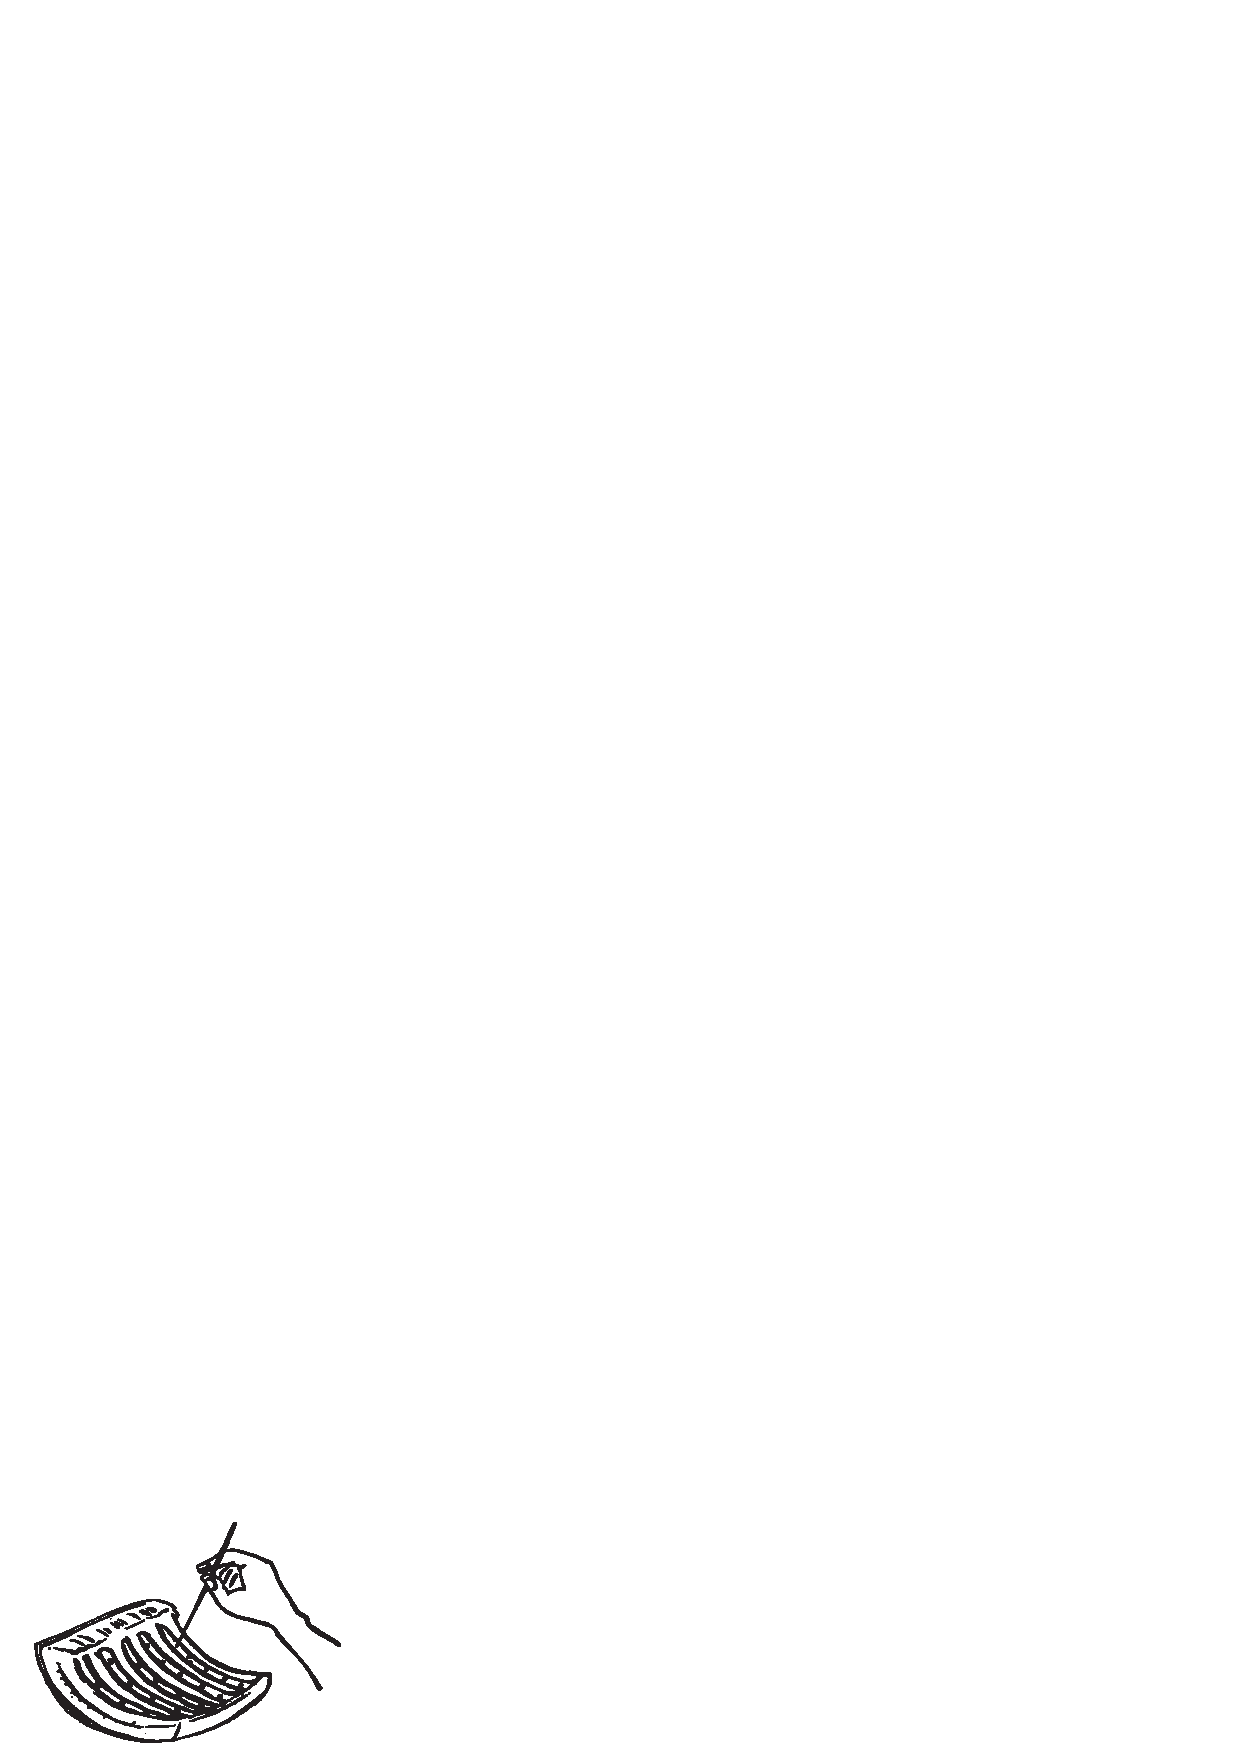
\includegraphics[scale=1]{illustration-005.pdf}%
\vspace{-.125\baselineskip}%
\caption{刺气眼}
\label{fig:poking-holes}
\end{wrapfigure}
宽九寸。肉皮须平整没有凸凹者。先去净茸毛,刮洗干净。然后肉皮向下、排骨向上放于
案板上,用直径二分粗的尖长竹签,在排骨缝中瘦肉上刺上若干气眼。刺的深度以接近肉
皮为合适,但不要把肉皮刺破(图\,\ref{fig:poking-holes}\,)。然后将它揩干水份,
用铁质二股烤叉一把,由排骨之下,肥肉之上的痩肉中叉进去(图\,%
\ref{fig:forking-meat}\,),叉尖伸出肉方外约一尺左右。

\begin{wrapfigure}[13]{r}{11em}%
\centering%
\vspace{-2\baselineskip}%
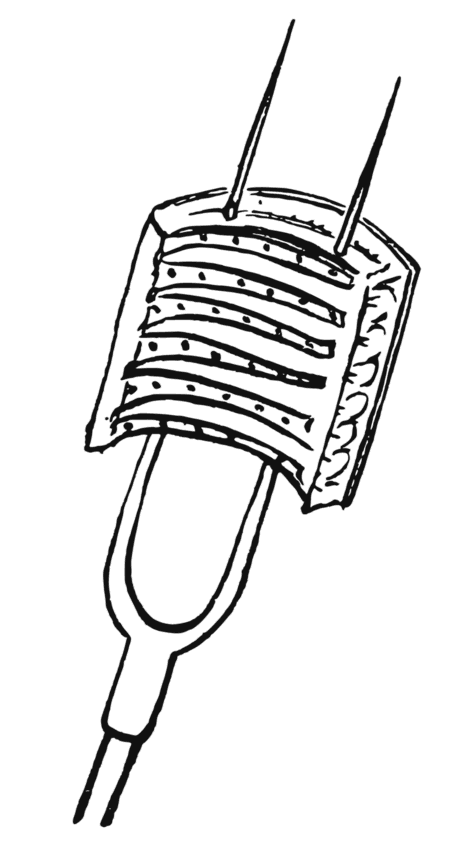
\includegraphics[scale=1]{illustration-006.pdf}%
\vspace{-.625\baselineskip}%
\caption{叉肉}
\label{fig:forking-meat}
\end{wrapfigure}
\vbadness=10000%

\step[出坯] 用干柴十斤,先用二斤放炉内烧燃,炉中火苗燎出炉口一尺至二尺(须经常
保持这种火苗,火苗不均匀时加柴),随即手拿叉柄,将肉方的皮向着火苗,排骨向上
(不要着火)在火苗上燎。一面调剂火候,一面手拿叉柄左右拧动。拧动的角度是:先把
肉方拧至肉皮与地平成八十五度后,再拧过去成同样的角度。这样反复来回拧动。拧动的
速度是:中间稍稍快,两端稍停。着重燎肉方的四周和四角,燎至肉皮上的毛眼中好像在
沸腾。同时猪皮上比较粗老的皮被烤成一层很薄的黑壳,自行整张地脱落于炉火中(若有
的地方没有落,就说明那里的火候还不够),然后将肉方挪开炉火,用净布擦净叉尖,取
下放入烫水中,用布帕洗净。通过出坯,肉皮比原肉皮薄,保留的肉皮约半分厚,皮上微
微现出蜂窝形状的花纹,带牙黄色,本道工序即成。待本菜上席前二十分钟再进行烤酥的
工序。

\step[烤酥] 用青砖二十四块,在平坦的地坪上嵌一烤池,用细煤渣灰五斤平铺在烤池底,
将杠炭八斤烧红,平放(不要
\begin{wrapfigure}[13]{l}{15em}%
\centering%
\vspace{-.5\baselineskip}%
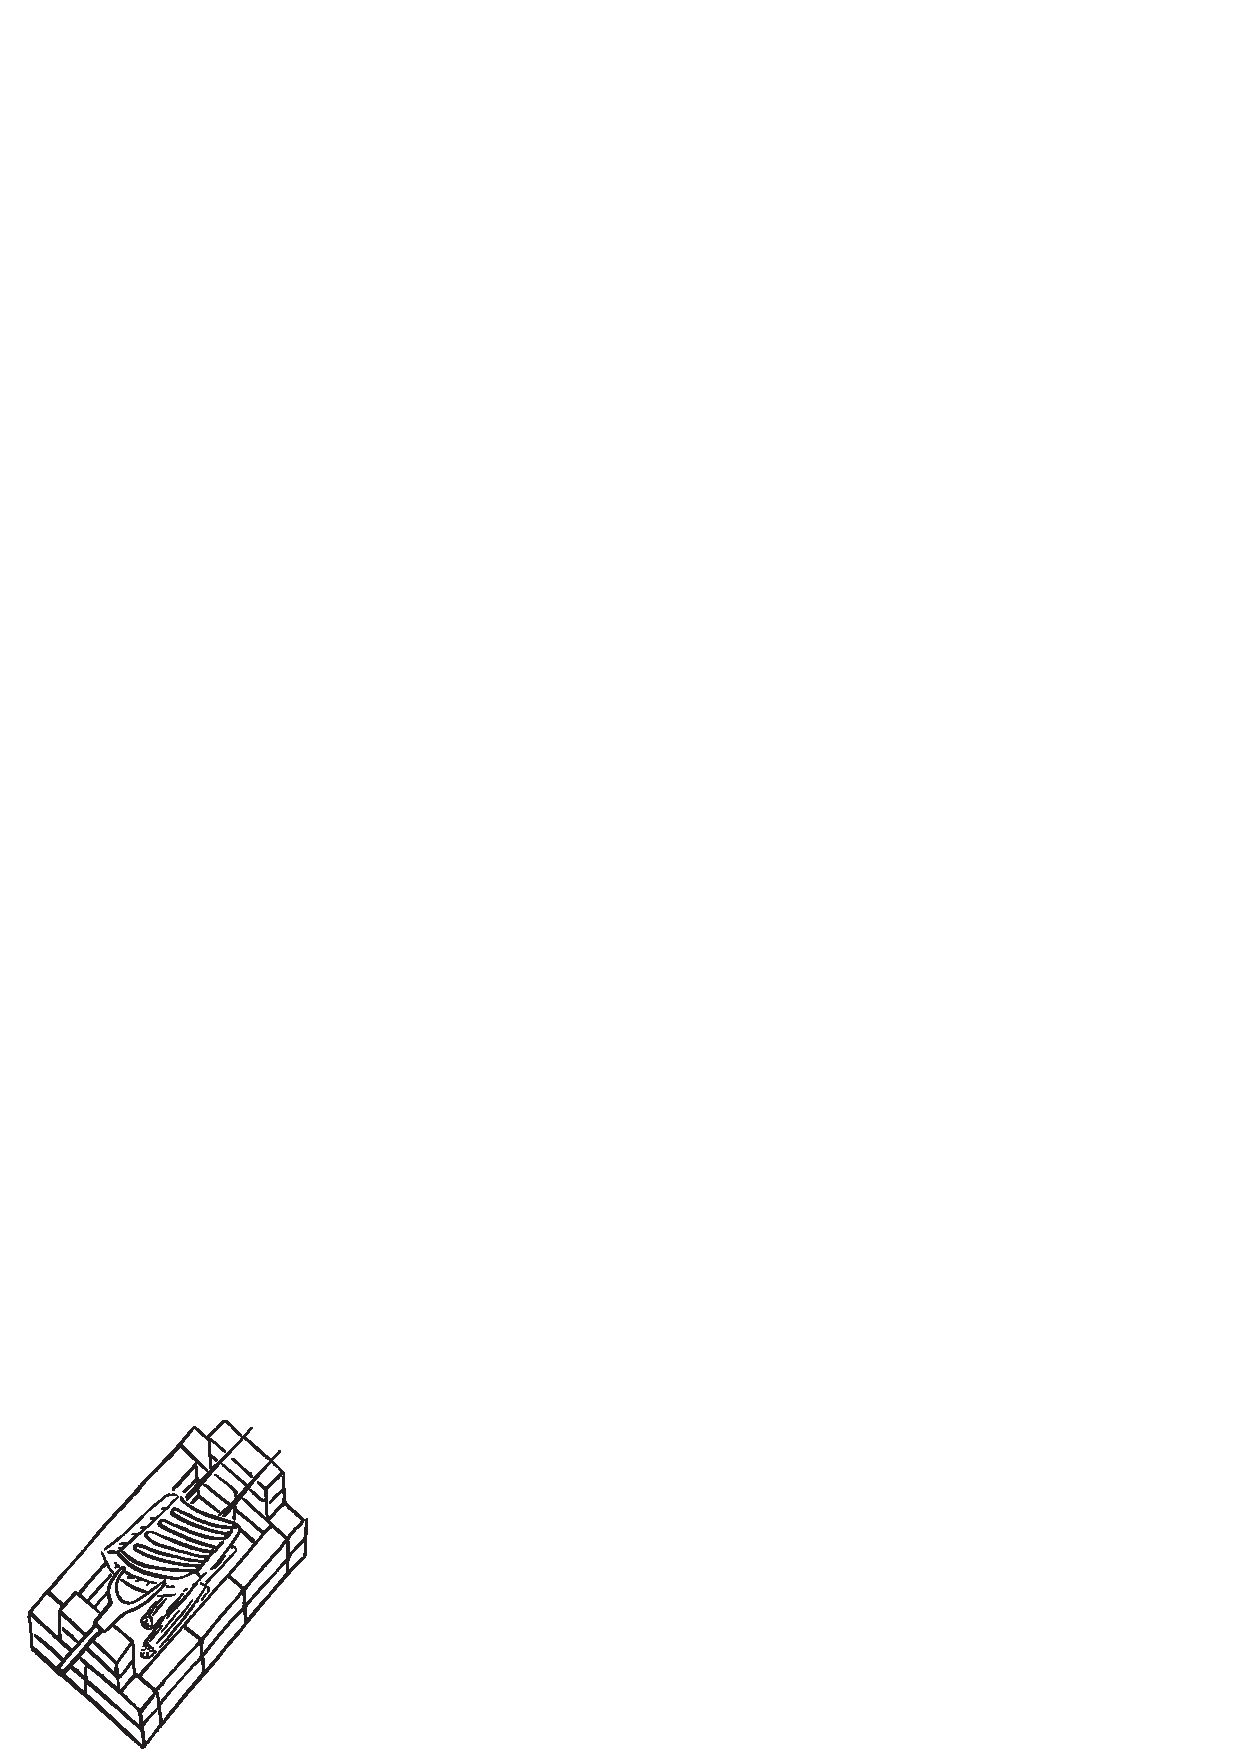
\includegraphics[scale=1]{illustration-007.pdf}%
\vspace{.1875\baselineskip}%
\caption{烤酥}
\label{fig:baking-meat}
\end{wrapfigure}
\vbadness=10000%
立放,立放便要伸出火苗,烤酥时严忌火苗)在烤池之中。再将肉方由原叉眼中叉好,放
于烤池上,肉皮向火,排骨向上(图\,\ref{fig:baking-meat}\,),同样手拿叉柄左右
拧动。拧动的角度与出坯相同,但速度稍快。烤至肉方出油时,将烤池内的红杠炭捡于烤
池四周(前后两端多放一些,去净池心的火星,以免肉方的油滴于火上,引起火苗),继
续拧动着烤。此时肉方皮上的油很多,为了使它在肉皮上流来流去,把皮烫酥,而不掉下
来,故拧动速度宜再快些。烤至肉皮成金黄色时,可以用刀尖试验一下是否酥泡。试法
是:用手指捏着刀叶,只留一分长的刀尖在外,将肉方拿离烤池,用刀尖在肉皮上连锥几
下,如发出酥泡的响声为合格。然后将香油三钱刷于酥皮之上,用净布擦净叉尖,取下酥
方,酥皮向上放于大圆盘中。

\step[铲皮上席] 用刀尖在酥皮下平铲,将铲下的酥皮切成一寸半长、七分宽的条方片,
照原样摆于肉方之上。另外,给每位顾客配汤盃一个,内盛加味特级清汤\footnotemark
(二两);三寸手碟一个,内盛蒜片、甜酱(甜酱中加香油二钱搅匀)、葱白段(一寸半
长)三段;再配五寸平盘一个,内盛点心两块,连同酥方一同上席。

\step[吃法] 一般只吃酥方皮,不吃肉。肉可用来做回锅肉,别有风味。

\suggestion

烤方需要一定技术,操作中稍不注意,就会发生质量事故。易于发生的质量事故及其补救
方法如下:

\hint[方皮鼓泡] 鼓泡在“出坯”和“烤酥”中都会发生。其原因是气眼刺得不好,或拧动角
度太大。补救方法是:把肉方拿离烤池,用尖头竹签在鼓泡的附近由痩肉中刺眼放气,若
鼓泡太大,可用刀将鼓泡的皮割去,抹上蛋清豆粉,稍抹厚点,再继续烤。

\hint[硬皮] 发生硬皮的原因是“出坯”时火候不匀,或烤酥时拧动角度太小。补救方法是:
将肉方拿离烤池,在池中捡红杠炭一块(炭的大小与硬皮相等),逼近硬皮处烤至微焦,
再用小刀将烤焦处之皮刮去一层,继续上烤池烤。

\hint[烂皮] 发生烂皮的原因是出坯时拧动速度太慢,以致肉皮被烧烂。补救方法:用蛋
清豆粉抹烂皮处,厚厚地抹一层,再继续上烤池烤。

\hint[漏油] 在选料或刺气眼没有注意,皮上有眼就会漏油。在烤酥时,可用蛋清团粉抹
严,再继续烤。

\features

此菜一般是高贵筵席的配菜,色彩金黄,美观大方,吃时酥香,脂肪特多,而爽口不腻。

\footnotetext{
\begin{subrecipe}{特级清汤}

\ingredients

\ingredient{老母鸡}{一只(三斤)}
\ingredient{老肥鸭}{一只(三斤)}
\ingredient{火腿蹄子}{一只}
\ingredient{火腿棒子骨}{一斤}
\ingredient{排骨}{二斤}
\ingredient{鸡脯肉}{三个}
\ingredient{猪生瘦肉}{五斤}
\ingredient{清水}{三十斤}

\preparation

\step 将鸡、鸭宰杀,去毛,去内脏。蹄子、棒子骨刮洗干净。生瘦肉、鸡脯肉都分别用
刀背捶成茸。

\step 汤锅放炉上,将棒子骨、排骨、蹄子、鸡、鸭依次放入汤锅中,倒入清水二十五
斤,用旺火烧开,去净泡沫,炖一小时。而后捞出,漂于温热水中。用猪肉茸一斤,加清
水一斤兑匀调散,倒入汤锅中;待瘦肉和泡沫浮起时,用漏瓢打净。将鸡、鸭、蹄、骨等
用热水洗净,放于汤锅中,用微火焅半小时,将鸡、鸭捞出另作别用,再将各骨捞出漂温
水中。然后将猪肉茸四斤,加清水三斤调散倒于汤锅中;待肉茸浮起时,用漏瓢把它挤成
四至五个肉饼。再将汤面浮油吹净,将各骨用温水洗净,轻轻放入汤锅中;随后将肉饼放
于各骨之上,用小微火焅。此时汤已变色,很象料酒颜色。鸡茸内加清水一斤调散。待使
用清汤时,再将鸡茸倒入汤中,待泡沫和肉茸浮起后,将泡沫和肉茸打去,即成清汤。
\end{subrecipe}
}

\end{recipe}

% vim: filetype=tex noautoindent nojoinspaces
% vim: fileencoding=utf-8 formatoptions+=m
% vim: textwidth=78 tabstop=4 shiftwidth=4 softtabstop=4

\vspace{1\baselineskip}
% BSD 3-Clause License
%
% Copyright (c) 2023, 2025 Quux System and Technology. All rights reserved.
%
% Redistribution and use in source and binary forms, with or without
% modification, are permitted provided that the following conditions are met:
%
% 1. Redistributions of source code must retain the above copyright notice, this
%    list of conditions and the following disclaimer.
%
% 2. Redistributions in binary form must reproduce the above copyright notice,
%    this list of conditions and the following disclaimer in the documentation
%    and/or other materials provided with the distribution.
%
% 3. Neither the name of the copyright holder nor the names of its
%    contributors may be used to endorse or promote products derived from
%    this software without specific prior written permission.
%
% THIS SOFTWARE IS PROVIDED BY THE COPYRIGHT HOLDERS AND CONTRIBUTORS "AS IS"
% AND ANY EXPRESS OR IMPLIED WARRANTIES, INCLUDING, BUT NOT LIMITED TO, THE
% IMPLIED WARRANTIES OF MERCHANTABILITY AND FITNESS FOR A PARTICULAR PURPOSE ARE
% DISCLAIMED. IN NO EVENT SHALL THE COPYRIGHT HOLDER OR CONTRIBUTORS BE LIABLE
% FOR ANY DIRECT, INDIRECT, INCIDENTAL, SPECIAL, EXEMPLARY, OR CONSEQUENTIAL
% DAMAGES (INCLUDING, BUT NOT LIMITED TO, PROCUREMENT OF SUBSTITUTE GOODS OR
% SERVICES; LOSS OF USE, DATA, OR PROFITS; OR BUSINESS INTERRUPTION) HOWEVER
% CAUSED AND ON ANY THEORY OF LIABILITY, WHETHER IN CONTRACT, STRICT LIABILITY,
% OR TORT (INCLUDING NEGLIGENCE OR OTHERWISE) ARISING IN ANY WAY OUT OF THE USE
% OF THIS SOFTWARE, EVEN IF ADVISED OF THE POSSIBILITY OF SUCH DAMAGE.
%
\begin{recipe}{叉烧奶猪}

\ingredients

\ingredient{乳猪一只}{约十三斤}
\ingredient{咸红酱油}{二两}
\ingredient{香油}{二两}
\ingredient{杠炭}{八斤}

\preparation

\step 饲养与宰杀:将乳猪买回,用稀饭喂养三四天,以去其腹内污秽和长膘。杀时用
尖刀从咽喉处杀死,倒提后足流去血浆。再用干细炭灰匀撒猪身以手抹匀,以六至七成开
的热水烫洗去毛,从头至尾用镊子(头部凹缝处可用烧红的铁钎烙)清洗干净。然后从喉
头起将猪逢中对半剖开,去肚腹内脏,留腰子不取。

\step 盘足:将两前足屈起,从挨近颈下裙边处(用尖刀在两边各挖一个孔)塞入腹腔。
另用筷子两支,削成竹钉,分别穿过猪蹄前端,以防烤时滑出腹外;后足亦如前法盘入腹
腔,用筷子穿好。

\step 出坯:在热水中将猪皮烫伸,取出用干净布抹干水气,再以红酱油将皮抹成黄红
色。此时从杀口处取出颈颡骨一节(约一寸长),再由腹腔内将脊椎与肋骨接榫处(俗呼
龙骨)从中切剖约二寸长,以便上叉时猪身平伏不致突起。

\step 上叉:将叉子(铁制、两股)从猪后腿近肘处刺入猪身,穿过腹腔,在一、二匹肋
骨缝中刺进猪肉层,再从猪头两耳根下穿出(此时叉尖约与猪眼平行);将两耳边用刀修
去一部分,使之直立略呈尖形;将尾巴用竹签穿过,扭成乙形,尾尖向上略微倾向猪头。
用尖头竹签,从肚腹两边裙边处刺进猪肉,以不伤皮为度。在肋缝处可以斜刺,大约每匹
肋骨刺三下即可,作用是避免烧烤时猪身皮面起泡。注意切勿将猪皮刺伤。

\step 烧烤:先砌砖池一个,长二尺五、宽二尺、高六寸五,池底垫细炭灰一层约五分厚。

\step 烤头:将杠炭烧红,置于砖池中央,将猪头向下,腹向池外,用火烤至头顶,烤到
脸泡成淡黄色,耳朵烤干为止。

\step 吊膛:将杠炭火勾平散开,把叉子头、尖,平放在砖池上。此时猪腹向下,烤至水
气吊干,以手触之无水份,不粘手为度。此时再将杠炭勾至砖池周围,中间不留炭火,杠
炭分布在叉柄叉尖两端占三分之二(即放猪头、尾处),两侧三分之一。烤时猪背向下,
腹向上。在往两侧翻动时,起初角度应稍大,至翻到裙边肉处。到裙边微带黄色时,角度
渐小,直到只翻烤背部。烤至全身火色均匀,均呈黄色时,再周身滚转烤,至烤成深琥珀
色为止,用筷子敲一下清脆作卜卜声。(翻烤时手要稳,火要匀,并密切注意如发生起泡
现象,必须立即将叉离开砖池,用竹签由腹腔内距起泡不远处刺进以泄其气。如任其爆烈
则吃时顶牙,影响质量。)

烤好后,将杠炭散开铺满砖池,将猪身抹上香油,在火上翻滚烤约四五遍离池。将叉尖用
布搽净,用手扶住猪身后肘将叉取出。

将烤好的猪放在干净案板上,用尖刀将猪皮划成长方形骨牌片。划时先从头至尾划直线,
后划横线。再用小刀启松,使皮、肉相离,但仍保持原形。随配点心二盘(荷叶饼、烧饼
均可),连同葱酱碟上席。

此菜一般食皮弃肉,亦有将腰子、耳朵、尾巴、脑花、水肉(即皮下之肉)另切一盘上席
者谓之“小件头”,吃法与上同。

\features

此菜系传统烧烤大菜,用于上等筵席。

\end{recipe}

% vim: filetype=tex noautoindent nojoinspaces
% vim: fileencoding=utf-8 formatoptions+=m
% vim: textwidth=78 tabstop=4 shiftwidth=4 softtabstop=4

\end{tocminipageright}

\addtocontents{toc}{\protect\enlargethispage{.5\baselineskip}}%
\category{鸡鸭类}
\setlength{\cookbookafterrecipeskip}{.6875\baselineskip plus 1.25\baselineskip}%

\begin{tocminipageleft}
\enlargethispage{-1\baselineskip}
\begin{recipe}{怪味鸡}

\ingredients

\ingredient{熟阉鸡腿}{一斤二两}
\ingredient{芝麻(两用)}{六钱}
\ingredient{葱白丁}{六钱}
\ingredient{白糖}{三钱}
\ingredient{花椒面}{一分}
\ingredient{醋}{三钱}
\ingredient{酱油}{一两五}
\ingredient{辣椒油}{六钱}
\ingredient{香油}{三钱}

\cooking

\step 取肥阉鸡腿,放入汤锅中加清水,将鸡腿淹没,先用旺火煮沸,再将汤锅挪到微火
上煮约二十分钟(在煨煮过程中水都要把鸡腿淹没,水不够时可加煮沸的汤)即熟。然后
捞起晾冷,去骨,砍成五分宽、七分长的斜象眼块(即斜方块)。用盘一个,盘中心先将
葱白丁放入,再将砍好的鸡块摆在上面,状如松果纹。
\step 芝麻用清水淘洗,去净空壳、沙石,滤干水;放入锅中置微火上,以手铲不停翻
炒,炒至发出“啪啪”的声音,呈金黄色(注意不要炒糊)时即铲入碗内。然后取用五钱放
在缽内,砸成粉,加香油调匀,成为芝麻酱。
\step 将芝麻酱、酱油、白糖、醋、辣椒油、花椒面等一并放入碗内调匀后,淋在摆好的
鸡块上;然后撒上余下的芝麻一钱即成。

\notes

此菜颜色红亮,质地细嫩,味鲜而不太辣,有强烈的麻辣香味。

\end{recipe}

% vim: filetype=tex noautoindent
% vim: fileencoding=utf-8
% vim: textwidth=78 tabstop=4 shiftwidth=4 softtabstop=4

\vspace{.3125\baselineskip}
\begin{recipe}{棒棒鸡丝}

\ingredients

\ingredient{生鸡肉}{一斤半}
\ingredient{香油}{一钱}
\ingredient{熟油辣椒}{五钱}
\ingredient{白糖}{二钱}
\ingredient{花椒面}{一分}
\ingredient{酱油}{一两}
\ingredient{芝麻酱}{二钱}
\ingredient{葱白}{一钱}
\ingredient{醋}{二钱}

\cooking

\step 	生鸡肉(选料以仔鸡为宜)在汤锅内煮熟后捞起(不 能煮粑),晾冷,用刀去骨,切成长二寸粗丝。葱白剖开切 成与鸡一样的丝子在盘内垫底,鸡丝铺在上面。

\step 	酱油、白糖、香油、芝麻酱、花椒面、醋、熟油辣椒 在碗内调匀,走桌时始将作料倒下,不宜过早。

\notes

肉质细嫩鲜美,味麻辣香咸,宜于佐酒。

\end{recipe}

% vim: filetype=tex noautoindent
% vim: fileencoding=utf-8
% vim: textwidth=78 tabstop=4 shiftwidth=4 softtabstop=4

\vspace{.3125\baselineskip}
\begin{recipe}[银芽拌鸡丝]{豆芽拌鸡丝}

\ingredients

\ingredient{熟鸡肉(去骨)}{五两}
\ingredient{绿豆芽}{二两}
\ingredient{酱油}{五钱}
\ingredient{辣椒油}{五钱}
\ingredient{白糖}{五分}
\ingredient{盐}{少许}
\ingredient{醋}{少许}
\ingredient{蒜泥}{少许}
\ingredient{味精}{少许}

\cooking

\step 豆芽淘洗干净,掐去两头。

\step 鸡肉切二粗丝,根条均匀。

\step 绿豆芽用沸水汆一下,立即捞起,造点毛毛盐,晾开餘冷,放入盘中作底。鸡丝放
面上,酱油、辣椒油、5示泥、:醋、白糖、味精等用碗调匀,淋于鸡丝面上即成。

\features

颜色红亮,味鲜而嫩,下酒的碟子菜。

\end{recipe}

% vim: filetype=tex noautoindent
% vim: fileencoding=utf-8 formatoptions+=m
% vim: textwidth=78 tabstop=4 shiftwidth=4 softtabstop=4

\begin{recipe}{自拌鸡丝}

\ingredients

\ingredient{去骨熟鸡(仔公鸡)}{一斤二两}
\ingredient{白糖}{五钱}
\ingredient{酱油}{一两五}
\ingredient{油辣椒}{一两}
\ingredient{蒜泥}{五钱}
\ingredient{窝油}{五钱}
\ingredient{香油}{五钱}
\ingredient{花椒面}{五分}
\ingredient{芝麻酱}{五钱}
\ingredient{味精}{三分}
\ingredient{白葱头}{二两}
\ingredient{芥末}{三钱}
\ingredient{醋}{三钱}

\preparation

\step 将鸡皮扯下,鸡骨剔尽,皮及肉分别切成二粗丝,鸡丝放入蓝色圆盘,鸡皮堆在上
面。

\step 葱头切成丝,窝油、酱油、醋、花椒面、蒜泥、白糖、味精、香油、芝麻酱、油辣
椒、芥末等分别盛入十二个碟子。

\features

满足顾客口味,自己掌握调料,宜下酒。

\end{recipe}

% vim: filetype=tex noautoindent nojoinspaces
% vim: fileencoding=utf-8 formatoptions+=m
% vim: textwidth=78 tabstop=4 shiftwidth=4 softtabstop=4

\begin{recipe}{}

\ingredients

\ingredient{}{}

\cooking

\step

\notes

\end{recipe}

% vim: filetype=tex noautoindent
% vim: fileencoding=utf-8
% vim: textwidth=78 tabstop=4 shiftwidth=4 softtabstop=4

\begin{recipe}{}

\ingredients

\ingredient{}{}

\cooking

\step

\notes

\end{recipe}

% vim: filetype=tex noautoindent
% vim: fileencoding=utf-8
% vim: textwidth=78 tabstop=4 shiftwidth=4 softtabstop=4

\begin{recipe}{}

\ingredients

\ingredient{}{}

\cooking

\step

\notes

\end{recipe}

% vim: filetype=tex noautoindent
% vim: fileencoding=utf-8
% vim: textwidth=78 tabstop=4 shiftwidth=4 softtabstop=4

\begin{recipe}{}

\ingredients

\ingredient{}{}

\cooking

\step

\notes

\end{recipe}

% vim: filetype=tex noautoindent
% vim: fileencoding=utf-8
% vim: textwidth=78 tabstop=4 shiftwidth=4 softtabstop=4

\begin{recipe}{陈皮鸡}

\ingredients

\ingredient{仔鸡}{(二斤半)一只}
\ingredient{姜}{三钱}
\ingredient{錯}{六分}
\ingredient{千辣椒}{六钱}
\ingredient{料酒}{二钱五}
\ingredient{陈皮}{二钱}
\ingredient{酱油}{二钱}
\ingredient{香油}{三钱}
\ingredient{花椒}{六分}
\ingredient{盐}{六分}
\ingredient{菜油}{二斤耗四两}
\ingredient{白糖}{二钱}
\ingredient{大葱}{一根}

\cooking

\step 选肥嫩仔鸡,宰杀后除净毛,砍去头足,除去内脏,剔除骨头。将鸡肉切成六、七
分大的小块,盛入大碗中。用拍松的姜、大葱放入鸡肉中,再加料酒、盐、酱油、一起拌
匀,稍醃后待用。

\step 白糖、醋、酱油放入小碗中搅匀,成汁待用6

\step 锅在火炉上烧红,倒入菜油二斤,在旺火上烧热。把鸡肉(拣去葱、姜)放入油内
炸五分钟左右,呈金黄色时捞出;泌去锅中余油,将锅仍放火炉上,再倒入菜油二两五烧
热,放入辣椒、花椒、陈皮稍炸,随即再倒下鸡块,炒匀后即烹入糖醋汁,再次炒匀起锅
入盘,淋上香油即成。

\features

麻辣香嫩,带陈皮味,为佐酒好菜。

\end{recipe}

% vim: filetype=tex noautoindent
% vim: fileencoding=utf-8 formatoptions+=m
% vim: textwidth=78 tabstop=4 shiftwidth=4 softtabstop=4

\begin{recipe}{溜珊瑚鸡丁}

\ingredients

\ingredient{母鸡脯}{五两}
\ingredient{盐}{五分}
\ingredient{水豆粉}{三钱}
\ingredient{红萝卜}{四两}
\ingredient{料酒}{三钱}
\ingredient{香油}{一分}
\ingredient{鸡蛋清}{一个}
\ingredient{化猪油}{六两耗二两}
\ingredient{干豆粉}{三钱}
\ingredient{味精}{二分}

\preparation

\step 鸡脯切成四分见方的丁,用蛋清豆粉、料酒、盐拌匀。

\step 红萝卜洗净去皮,用筷子刮萝卜成茸,心子不用。

\step 化猪油在旺火上娆至七成火,即将拌芡的鸡丁倒下,妙散,泌去油;锅内留油二两
,即将红萝卜茸熵出红色后,连同鸡丁炒匀,立即烹入料酒、盐、豆粉兑成的滋汁,即起
锅,同时淋香油少许。

\features

质地细嫩,味鲜美,鸡丁呈珊瑚色。

\end{recipe}

% vim: filetype=tex noautoindent
% vim: fileencoding=utf-8 formatoptions+=m
% vim: textwidth=78 tabstop=4 shiftwidth=4 softtabstop=4

\begin{recipe}{溜鸡米}

\ingredients

\ingredient{净鸡脯肉}{五两}
\ingredient{慈菇}{二两}
\ingredient{熟火腿}{一两}
\ingredient{白葱头}{一钱}
\ingredient{盐}{三分}
\ingredient{料酒}{二钱}
\ingredient{鸡蛋清}{一个}
\ingredient{干豆粉}{三钱}
\ingredient{水豆粉}{一钱}
\ingredient{味精}{一分}
\ingredient{胡椒面}{一分}
\ingredient{清汤}{一两}
\ingredient{香油或鸡油}{一钱}
\ingredient{化猪油}{四两耗一两五}

\preparation

\step 鸡脯肉切成如绿豆米大的丁,慈菇削去皮,火腿、整葱亦分别切成如绿豆米大的丁
,鸡蛋合干豆粉搅成蛋清豆粉,盐、料酒、水豆粉、味精、胡椒面、清汤合兑成滋汁。

\step 鸡肉丁用蛋清豆粉、盐、料酒拌和均匀,即投入炙过的五成热的油锅,用筷子滑散
,即投入火腿、茨菇,再滑散后将锅提离火口,泌去油剩约一两,再将锅放在火上,把各
丁拨在一边,放入葱末一煸,然后动作要快,烹入滋汁,用瓢浪一转,加香油或鸡油起锅
,盛入深色条盘。

\features

颜色调和,鲜嫩味美,酒饭均宜。

\end{recipe}

% vim: filetype=tex noautoindent nojoinspaces
% vim: fileencoding=utf-8 formatoptions+=m
% vim: textwidth=78 tabstop=4 shiftwidth=4 softtabstop=4

\begin{recipe}{家常鸡丝}

\ingredients

\ingredient{仔鸡肉(净)}{五两}
\ingredient{混合油}{二两五}

\ingredient{芹菜}{八两}
\ingredient{料酒}{四钱}
\ingredient{蒜苗}{一两}
\ingredient{酱油}{三钱}
\ingredient{豆瓣}{八钱}
\ingredient{水豆粉}{三分}
\ingredient{仔姜}{一钱}
\ingredient{醋}{少许}

\preparation

\step 芹菜只掐嫩心部分,去叶抽筋,蒜苗去鬚、去黄叶,均淘洗干净,用刀分别正切成
一寸长的节,蒜苗头划成四瓣,仔姜切成细丝,豆瓣剁碎,鸡肉切成一寸五长的二粗丝。

\step 」昆合油在锅内烧至六成火候,即将鸡丝倒下,熵干水气,炒散后(刚干水气,不
能煸干)倒豆瓣、姜丝,熵出香味即下料酒与鸡丝,共同炒匀后,芹黄、蒜苗一齐倒下,
再连炒几下。起锅时勾少许清芡及醋。

\features

此菜富家常味,辣香细嫩,酒饭均宜。

\end{recipe}

% vim: filetype=tex noautoindent
% vim: fileencoding=utf-8 formatoptions+=m
% vim: textwidth=78 tabstop=4 shiftwidth=4 softtabstop=4

% BSD 3-Clause License
%
% Copyright (c) 2023 Quux System and Technology. All rights reserved.
%
% Redistribution and use in source and binary forms, with or without
% modification, are permitted provided that the following conditions are met:
%
% 1. Redistributions of source code must retain the above copyright notice, this
%    list of conditions and the following disclaimer.
%
% 2. Redistributions in binary form must reproduce the above copyright notice,
%    this list of conditions and the following disclaimer in the documentation
%    and/or other materials provided with the distribution.
%
% 3. Neither the name of the copyright holder nor the names of its
%    contributors may be used to endorse or promote products derived from
%    this software without specific prior written permission.
%
% THIS SOFTWARE IS PROVIDED BY THE COPYRIGHT HOLDERS AND CONTRIBUTORS "AS IS"
% AND ANY EXPRESS OR IMPLIED WARRANTIES, INCLUDING, BUT NOT LIMITED TO, THE
% IMPLIED WARRANTIES OF MERCHANTABILITY AND FITNESS FOR A PARTICULAR PURPOSE ARE
% DISCLAIMED. IN NO EVENT SHALL THE COPYRIGHT HOLDER OR CONTRIBUTORS BE LIABLE
% FOR ANY DIRECT, INDIRECT, INCIDENTAL, SPECIAL, EXEMPLARY, OR CONSEQUENTIAL
% DAMAGES (INCLUDING, BUT NOT LIMITED TO, PROCUREMENT OF SUBSTITUTE GOODS OR
% SERVICES; LOSS OF USE, DATA, OR PROFITS; OR BUSINESS INTERRUPTION) HOWEVER
% CAUSED AND ON ANY THEORY OF LIABILITY, WHETHER IN CONTRACT, STRICT LIABILITY,
% OR TORT (INCLUDING NEGLIGENCE OR OTHERWISE) ARISING IN ANY WAY OUT OF THE USE
% OF THIS SOFTWARE, EVEN IF ADVISED OF THE POSSIBILITY OF SUCH DAMAGE.
%
\begin{recipe}{兰花鸡丝}

\ingredients

\ingredient{鸡脯肉}{五两}
\ingredient{兰花}{二十件}
\ingredient{鸡蛋清}{二个}
\ingredient{味精}{二分}
\ingredient{清汤}{一两五}
\ingredient{干豆粉}{一两}
\ingredient{化猪油}{一斤耗三两}
\ingredient{盐}{三分}
\ingredient{料酒}{二钱}

\preparation

\step 鸡脯肉洗净,切成二寸长细丝,用蛋清豆粉加盐、料酒拌和均匀。

\step 兰花去茎抽心,淘洗干净,用清水漂起。

\step 旺火先将锅炙后,猪油烧至四成火成温热油,将鸡丝倒下,用筷子滑散,将油滗
尽,再加入兰花、味精及剩余的盐和料酒,在锅内炒匀,加清汤,勾清芡,簸匀起锅。

\features

色白、味鲜,有自然花香。

\end{recipe}

% vim: filetype=tex noautoindent nojoinspaces
% vim: fileencoding=utf-8 formatoptions+=m
% vim: textwidth=78 tabstop=4 shiftwidth=4 softtabstop=4

% BSD 3-Clause License
%
% Copyright (c) 2023 Quux System and Technology. All rights reserved.
%
% Redistribution and use in source and binary forms, with or without
% modification, are permitted provided that the following conditions are met:
%
% 1. Redistributions of source code must retain the above copyright notice, this
%    list of conditions and the following disclaimer.
%
% 2. Redistributions in binary form must reproduce the above copyright notice,
%    this list of conditions and the following disclaimer in the documentation
%    and/or other materials provided with the distribution.
%
% 3. Neither the name of the copyright holder nor the names of its
%    contributors may be used to endorse or promote products derived from
%    this software without specific prior written permission.
%
% THIS SOFTWARE IS PROVIDED BY THE COPYRIGHT HOLDERS AND CONTRIBUTORS "AS IS"
% AND ANY EXPRESS OR IMPLIED WARRANTIES, INCLUDING, BUT NOT LIMITED TO, THE
% IMPLIED WARRANTIES OF MERCHANTABILITY AND FITNESS FOR A PARTICULAR PURPOSE ARE
% DISCLAIMED. IN NO EVENT SHALL THE COPYRIGHT HOLDER OR CONTRIBUTORS BE LIABLE
% FOR ANY DIRECT, INDIRECT, INCIDENTAL, SPECIAL, EXEMPLARY, OR CONSEQUENTIAL
% DAMAGES (INCLUDING, BUT NOT LIMITED TO, PROCUREMENT OF SUBSTITUTE GOODS OR
% SERVICES; LOSS OF USE, DATA, OR PROFITS; OR BUSINESS INTERRUPTION) HOWEVER
% CAUSED AND ON ANY THEORY OF LIABILITY, WHETHER IN CONTRACT, STRICT LIABILITY,
% OR TORT (INCLUDING NEGLIGENCE OR OTHERWISE) ARISING IN ANY WAY OUT OF THE USE
% OF THIS SOFTWARE, EVEN IF ADVISED OF THE POSSIBILITY OF SUCH DAMAGE.
%
\begin{recipe}{贵州鸡}

\ingredients

\ingredient{生鸡脯肉}{六两}
\ingredient{干海椒}{五钱}
\ingredient{鸡蛋}{二个}
\ingredient{姜}{二钱}
\ingredient{葱}{五钱}
\ingredient{蒜}{一钱}
\ingredient{料酒}{五钱}
\ingredient{酱油}{三钱}
\ingredient{盐}{三分}
\ingredient{干豆粉}{八钱}
\ingredient{白糖}{五分}
\ingredient{味精}{二分}
\ingredient{化猪油}{一斤耗三两}
\ingredient{清汤}{一两}

\preparation

\step 先将鸡脯肉用刀两边相对𠟤成交差形的花纹,再切成四分见方的鸡丁,放入料酒、
盐拌和均匀,放入碗内待用。

\step 将干海椒去把,放在开水内发胀,舂茸,再将姜蒜切成片,葱切成马耳朵形,分开
放入碗内待用。

\step 将鸡蛋及豆粉拌成蛋清豆粉,鸡丁同蛋清豆粉拌匀;再将锅放于旺火上烧红,放入
化猪油,烧至三成火后用手将调好的鸡丁抖入锅内,用竹筷滑散,搛入盘内。撇去锅内的
余油,留一两五油在锅内,放入姜、葱、蒜片及海椒茸,炒散;再放入料酒、味精、盐、
白糖、清汤、酱油,炒匀;再将盘内的鸡丁,倒入锅内,稍拨几转起锅即成。

\features

此菜色红、鲜嫩、味浓,适宜酒肴。

\end{recipe}

% vim: filetype=tex noautoindent nojoinspaces
% vim: fileencoding=utf-8 formatoptions+=m
% vim: textwidth=78 tabstop=4 shiftwidth=4 softtabstop=4

% BSD 3-Clause License
%
% Copyright (c) 2023 Quux System and Technology. All rights reserved.
%
% Redistribution and use in source and binary forms, with or without
% modification, are permitted provided that the following conditions are met:
%
% 1. Redistributions of source code must retain the above copyright notice, this
%    list of conditions and the following disclaimer.
%
% 2. Redistributions in binary form must reproduce the above copyright notice,
%    this list of conditions and the following disclaimer in the documentation
%    and/or other materials provided with the distribution.
%
% 3. Neither the name of the copyright holder nor the names of its
%    contributors may be used to endorse or promote products derived from
%    this software without specific prior written permission.
%
% THIS SOFTWARE IS PROVIDED BY THE COPYRIGHT HOLDERS AND CONTRIBUTORS "AS IS"
% AND ANY EXPRESS OR IMPLIED WARRANTIES, INCLUDING, BUT NOT LIMITED TO, THE
% IMPLIED WARRANTIES OF MERCHANTABILITY AND FITNESS FOR A PARTICULAR PURPOSE ARE
% DISCLAIMED. IN NO EVENT SHALL THE COPYRIGHT HOLDER OR CONTRIBUTORS BE LIABLE
% FOR ANY DIRECT, INDIRECT, INCIDENTAL, SPECIAL, EXEMPLARY, OR CONSEQUENTIAL
% DAMAGES (INCLUDING, BUT NOT LIMITED TO, PROCUREMENT OF SUBSTITUTE GOODS OR
% SERVICES; LOSS OF USE, DATA, OR PROFITS; OR BUSINESS INTERRUPTION) HOWEVER
% CAUSED AND ON ANY THEORY OF LIABILITY, WHETHER IN CONTRACT, STRICT LIABILITY,
% OR TORT (INCLUDING NEGLIGENCE OR OTHERWISE) ARISING IN ANY WAY OUT OF THE USE
% OF THIS SOFTWARE, EVEN IF ADVISED OF THE POSSIBILITY OF SUCH DAMAGE.
%
\begin{recipe}[钢铁仔鸡]{海椒香辣鸡}

\ingredients

\ingredient{仔鸡一只}{二斤}
\ingredient{菜油}{四两}
\ingredient{干辣椒}{五钱}
\ingredient{豆瓣}{五钱}
\ingredient{花椒粒}{五分}
\ingredient{辣椒面}{三分}
\ingredient{味精}{二分}
\ingredient{酱油}{五钱}
\ingredient{料酒}{五钱}
\ingredient{盐}{二分}
\ingredient{姜}{一钱}
\ingredient{大蒜}{一钱}
\ingredient{蒜苗}{一两}
\ingredient{清汤}{二两}
\ingredient{香油}{五分}

\preparation

\step 鸡宰杀后去血退毛,去头足四大骨,清洗干净,将鸡连骨砍成四分见方的丁,放入
碗内待用;将蒜苗切成四分长的节,姜、蒜切成薄片,干辣椒切成节,分别放入盘内待
用。

\step 菜油四两在锅内烧至五成火,放入干辣椒微炒,再投入砍好的鸡炒数转(水气炒
干)后,依次放入豆瓣、辣椒面、姜、蒜、料酒、酱油、味精、花椒等,铲动数转,煵好
后再将清汤倒入锅内,待汤收干,放下蒜苗微炒数转,淋入香油,起锅即成。

\features

香辣,味浓,适宜佐酒。

\end{recipe}

% vim: filetype=tex noautoindent nojoinspaces
% vim: fileencoding=utf-8 formatoptions+=m
% vim: textwidth=78 tabstop=4 shiftwidth=4 softtabstop=4

\begin{recipe}{旱蒸全鸡}

\ingredients

\ingredient{活鸡一只}{约三斤}
\ingredient{𰪿糟浮子}{一两}
\ingredient{盐}{三钱}
\ingredient{花权}{数粒}
\ingredient{葱白}{二钱}
\ingredient{姜}{一钱}
\ingredient{生鸡油}{一两}

\preparation

\step 杀鸡、去毛、去脏腹、去足爪,出一水,将血水提净,除净细毛,全身抹盐和𰪿糟
浮子;加葱、姜、花椒、生鸡油等,用大鱼碗盛起。

\step 用小木甑一个,将篦子翻转垫平;锅内将水烧沸,木甑放上,鸡碗置甑内;再用尖
底瓦盆一个,盛清水放木甑上作盖,甑口处用湿布帕密封;用中武火使水保持沸变;由于
密封热气不易散发,水蒸汽上升到盆底结成水珠,滴于碗内成汤汁;约三小时鸡妃出甑,
翻入深边圆盘,连原汁蒸汤上席。

\features

鲜香、肥嫩、原汁原味、极富营养。

\end{recipe}

% vim: filetype=tex noautoindent nojoinspaces
% vim: fileencoding=utf-8 formatoptions+=m
% vim: textwidth=78 tabstop=4 shiftwidth=4 softtabstop=4

\begin{recipe}{三菌炖鸡}

\ingredients

\ingredient{仔鸡}{一斤半}
\ingredient{盐}{一钱五}
\ingredient{二汤}{二斤}
\ingredient{大葱}{三钱}
\ingredient{新鲜三菌\footnotemark}{一斤}
\ingredient{蒜}{二两五}
\ingredient{姜}{三钱}
\ingredient{化猪油}{二两}

\cooking

\step 三菌刮去菌身的粗皮和杂质,撕去老筋,除去菌足,淘洗干净;将菌顶大者切成四
牙,小者切成三牙;菌茎撕成两半,切成长一寸二分的段,用清水漂起。肥仔鸡连骨砍成
七分大的块。姜洗净,拍松,大葱去须,洗净。

\step 炒锅放炉上,放入猪油在锅内烧红,把姜、大葱、鸡块放入炒熟,加二汤、蒜等烧
开,舀入砂锅内用微火煨四十分钟左右。将三菌捞出滤干水气,再以猪油在炒锅内煸二分
钟后,仍倒入砂锅内,加盐,再用微火煨二十分钟,连汤带菜一起盛入碗中上席。

\features

此菜系汤菜,呈白色,鸡圯菌嫩,汤味鲜美。

\footnotetext{
三菌属于菌科,其形如伞,色白细嫩,味极鲜美,盛产于成都近郊。
}

\end{recipe}

% vim: filetype=tex noautoindent
% vim: fileencoding=utf-8 formatoptions+=m
% vim: textwidth=78 tabstop=4 shiftwidth=4 softtabstop=4

\begin{recipe}[生烧大转弯]{生烧鸡翅}

\ingredients

\ingredient{公鸡翅八对}{约一半}
\ingredient{水发口茉}{一两八}
\ingredient{冬笋剥皮去根}{二两五}
\ingredient{葱白}{六钱}
\ingredient{料酒}{一两五}
\ingredient{酱油}{三钱}
\ingredient{味精}{一分五}
\ingredient{化猪油}{一两}
\ingredient{火腿}{六钱}
\ingredient{盐}{一分五}
\ingredient{姜}{一钱五}
\ingredient{水豆粉}{二钱}
\ingredient{鸡汤}{一斤}
\ingredient{香油}{二钱}

\preparation

\step 将宰好去毛的生公鸡,用刀齐鸡身取下翅膀八对,洗净揩干,在酒精火上燎去细
毛,切去翅尖部分不用;每个翅膀从关节上一点切成两段(两段长短大致相等),再去
掉两头关节骨,放入锅内煮三分钟捞出,除去血腥水。火腿切成一寸长、两分宽、一分
厚的片。冬笋切成一寸长、宽厚各二分的片。口茉大的可用刀对切成两瓣。

\step 猪油放入锅内置于旺火上,将拍松的姜及葱白、料酒、鸡翅倒入锅内稍煵(约三分
钟),再加入酱油、盐和鸡汤等,烧开后用汤瓢撇去浮沫,倒入另外一个锅内,用微火烧
约一点半钟。直至肉将离骨而未离骨时,去掉姜、葱,再倾入炒锅内,即放味精及水豆
粉、勾芡,起锅时淋下香油上盘。

\features

此菜选料为鸡全身的活动部分,再经生烧久焖,入口更觉稠烂香嫩,色鲜味浓,非常可口。

\end{recipe}

% vim: filetype=tex noautoindent nojoinspaces
% vim: fileencoding=utf-8 formatoptions+=m
% vim: textwidth=78 tabstop=4 shiftwidth=4 softtabstop=4

\end{tocminipageleft}
\begin{tocminipageright}
\begin{recipe}{生烧鸡腿}

\ingredients

\ingredient{母鸡腿}{二十只}
\ingredient{盐}{二钱}
\ingredient{鸡油}{五钱}
\ingredient{清水}{二斤}
\ingredient{酱油}{一两五}
\ingredient{白糖}{五钱}
\ingredient{水豆粉}{二钱}
\ingredient{葱}{三钱}
\ingredient{干口笨}{三钱}
\ingredient{料酒}{五钱}
\ingredient{姜}{二钱}

\preparation

\step 将胡琴把子大小匀净鸡腿,拈净残毛,淘洗干净;姜拍破;葱挽成结;口茉用沸水
发胀,洗净,大朵的用刀切成两瓣。

\step 用包罐装清水下鸡腿,煮沸打净血泡,加葱、姜、料酒、糖汁、酱油、盐,在文火
上烧至鸡肉离骨,再加入口茉烧妃,即拈入条盘砌好,滋汁泌入炒锅内,勾芡,将鸡油淋
在鸡腿上即成。

\features

色金黄,昧鲜美细嫩〇

\end{recipe}

% vim: filetype=tex noautoindent
% vim: fileencoding=utf-8 formatoptions+=m
% vim: textwidth=78 tabstop=4 shiftwidth=4 softtabstop=4

\begin{recipe}{}

\ingredients

\ingredient{}{}

\cooking

\step

\notes

\end{recipe}

% vim: filetype=tex noautoindent
% vim: fileencoding=utf-8
% vim: textwidth=78 tabstop=4 shiftwidth=4 softtabstop=4

\begin{recipe}{福建仔鸡}

\ingredients

\ingredient{嫩仔鸡一只}{二斤半}
\ingredient{花椒}{六分}
\ingredient{姜}{二钱}
\ingredient{葱}{五钱}
\ingredient{料酒}{三钱}
\ingredient{盐}{七分}
\ingredient{酱油}{五钱}
\ingredient{白糖}{三钱}
\ingredient{胡椒面}{三分}
\ingredient{味精}{三分}
\ingredient{耢糟}{五钱}
\ingredient{香油}{一‘两}
\ingredient{清汤}{四两}
\ingredient{菜油}{一斤半耗二两}

\cooking

\step 	仔鸡宰杀后去血退毛,清洗干净,从背脊部砍开,挖 去内脏,去掉足爪不用,再清洗一次。再用刀尖将鸡脯及鸡 腿的肉剖开,把腿、翅、骨微微宰断,用手将盐、葱、姜、 酱油、耢糟、料酒、花椒等抹在鸡的内外,抹勻,渍一小时。

\step 	将锅放在旺火上,倒下菜油,烧至八、九成热时将鸡 取出搽干(原汁留用〉,投入油锅内炸熟炸透;泌去余油,将 抹鸡时的原汁一并倒入锅内,放下胡椒、白糖、香油、味精、 清汤,将锅内的滋汁收至一半为止,然后将鸡捞起放在墩子 上宰成一寸二长、五分宽的长方块,按照鸡的原形摆入盘内

(鸡脯向上〉。将锅内滋汁泌入碗内,将碗内的姜、葱、花 椒捞出剁成细末后在滋汁碗内调匀,淋于鸡脯的面上即成。

\notes

此菜鲜嫩可口,甜咸中带有麻味,四季均宜。

\end{recipe}

% vim: filetype=tex noautoindent
% vim: fileencoding=utf-8
% vim: textwidth=78 tabstop=4 shiftwidth=4 softtabstop=4

\begin{recipe}[喇嘛仔鸡]{香炸仔鸡}

\ingredients

\ingredient{仔鸡一只}{约二斤半}
\ingredient{鸡蛋}{三个}
\ingredient{生菜}{三两}
\ingredient{花椒}{约十粒}
\ingredient{香油}{五钱}
\ingredient{盐}{三分}
\ingredient{料酒}{五钱}
\ingredient{白糖}{三钱}
\ingredient{蕃茄酱}{五钱}
\ingredient{酱油}{五钱}
\ingredient{葱段}{五钱}
\ingredient{姜}{三钱}
\ingredient{醋}{三钱}
\ingredient{干豆粉}{一两五}
\ingredient{菜油}{二斤耗二两}

\preparation

\step 鸡宰杀后,净毛,从背上剖开,去腹,去头足,洗净滤干,盛入大碗;用酱油、
盐、料酒、姜、葱、花椒,在鸡身内外抹匀,待三十分钟左右上笼蒸好,蒸到“肉松翅
散”时取出晾冷;即将鸡骨全身去净,鸡蛋调成蛋清豆粉,于鸡肉上抹匀。

\step 菜油在锅内烧至七成火候,将鸡放入炸成金黄色,将油泌尽,淋上香油簸匀擀起
来,砍成大一字条盛入盘的端,另一端放生菜即成。

\features

色泽光润,味道脆嫩。

\end{recipe}

% vim: filetype=tex noautoindent nojoinspaces
% vim: fileencoding=utf-8 formatoptions+=m
% vim: textwidth=78 tabstop=4 shiftwidth=4 softtabstop=4

\begin{recipe}{}

\ingredients

\ingredient{}{}

\cooking

\step

\notes

\end{recipe}

% vim: filetype=tex noautoindent
% vim: fileencoding=utf-8
% vim: textwidth=78 tabstop=4 shiftwidth=4 softtabstop=4

\begin{recipe}{雪花鸡淖(闹)}

\ingredients

\ingredient{鸡脯}{三两}
\ingredient{胡椒面}{一分}
\ingredient{鸡蛋清}{四个}
\ingredient{味精}{二分}
\ingredient{熟瘦火腿.}{二钱}
\ingredient{料酒}{二钱}

\ingredient{干豆粉}{五钱}
\ingredient{鸡汤}{五两}
\ingredient{盐}{五分}
\ingredient{化猪油}{四两}

\cooking

\step 火腿剁为细末成“蒙子”。

\step 鸡脯在墩子上用刀背反复砸茸,边砸边用刀口剔去白 筋;鸡蛋清用筷子搅散,鸡茸在碗内用冷鸡汤解散,连同鸡 蛋清加料酒、盐、胡椒面、味精、水豆粉,搅匀成鸡浆。

\step 炒锅在旺火上将油烧至八成火候,即将鸡浆倒入,用 瓢子轻轻搅几转,再造动炒熟,入盘内,撒上火腿蒙子即成。

\notes

色白如雪,鲜嫩营养。

\end{recipe}

% vim: filetype=tex noautoindent
% vim: fileencoding=utf-8
% vim: textwidth=78 tabstop=4 shiftwidth=4 softtabstop=4

\begin{recipe}{}

\ingredients

\ingredient{}{}

\cooking

\step

\notes

\end{recipe}

% vim: filetype=tex noautoindent
% vim: fileencoding=utf-8
% vim: textwidth=78 tabstop=4 shiftwidth=4 softtabstop=4

\begin{recipe}{}

\ingredients

\ingredient{}{}

\cooking

\step

\notes

\end{recipe}

% vim: filetype=tex noautoindent
% vim: fileencoding=utf-8
% vim: textwidth=78 tabstop=4 shiftwidth=4 softtabstop=4

% BSD 3-Clause License
%
% Copyright (c) 2023 Quux System and Technology. All rights reserved.
%
% Redistribution and use in source and binary forms, with or without
% modification, are permitted provided that the following conditions are met:
%
% 1. Redistributions of source code must retain the above copyright notice, this
%    list of conditions and the following disclaimer.
%
% 2. Redistributions in binary form must reproduce the above copyright notice,
%    this list of conditions and the following disclaimer in the documentation
%    and/or other materials provided with the distribution.
%
% 3. Neither the name of the copyright holder nor the names of its
%    contributors may be used to endorse or promote products derived from
%    this software without specific prior written permission.
%
% THIS SOFTWARE IS PROVIDED BY THE COPYRIGHT HOLDERS AND CONTRIBUTORS "AS IS"
% AND ANY EXPRESS OR IMPLIED WARRANTIES, INCLUDING, BUT NOT LIMITED TO, THE
% IMPLIED WARRANTIES OF MERCHANTABILITY AND FITNESS FOR A PARTICULAR PURPOSE ARE
% DISCLAIMED. IN NO EVENT SHALL THE COPYRIGHT HOLDER OR CONTRIBUTORS BE LIABLE
% FOR ANY DIRECT, INDIRECT, INCIDENTAL, SPECIAL, EXEMPLARY, OR CONSEQUENTIAL
% DAMAGES (INCLUDING, BUT NOT LIMITED TO, PROCUREMENT OF SUBSTITUTE GOODS OR
% SERVICES; LOSS OF USE, DATA, OR PROFITS; OR BUSINESS INTERRUPTION) HOWEVER
% CAUSED AND ON ANY THEORY OF LIABILITY, WHETHER IN CONTRACT, STRICT LIABILITY,
% OR TORT (INCLUDING NEGLIGENCE OR OTHERWISE) ARISING IN ANY WAY OUT OF THE USE
% OF THIS SOFTWARE, EVEN IF ADVISED OF THE POSSIBILITY OF SUCH DAMAGE.
%
\begin{recipe}{芙蓉鸡片}

\ingredients

\ingredient{鸡脯肉}{三两}
\ingredient{鸡蛋}{六个}
\ingredient{水豆粉}{六钱}
\ingredient{味精}{三分}
\ingredient{料酒}{五钱}
\ingredient{盐}{四分}
\ingredient{水发口蘑}{二钱}
\ingredient{鲜笋}{四钱}
\ingredient{火腿}{三钱}
\ingredient{豌豆尖苞}{十余根}
\ingredient{化猪油}{四两}
\ingredient{鸡汤}{五两}
\ingredient{熟鸡皮}{一两}
\ingredient{鸡化油}{五钱}

\preparation

\step 先将鸡脯肉清洗干净,在墩子上捶茸后放在碗内;用二两鸡汤解散,投入豆粉、味
精、盐、料酒搅匀;将六个鸡蛋的蛋清投入解散的鸡茸内搅匀待用。

\step 将锅放在旺火上,倒下化猪油,烧至六成热时滗去油,用汤瓢将搅好的鸡茸舀入油
锅,摊成直径八寸、厚五厘的圆片,铲起放入盛有二汤的碗内;将鸡茸一直照样摊完(共
八片),放入碗内待用。

\step 火腿、口蘑、鲜笋、鸡皮都切成棋子块的小片。将锅放在火炉上,下猪油,倒入火
腿、口蘑、鲜笋、鸡皮、豌豆尖苞,炒动几转,倒下鸡汤四两,勾芡,然后将泡在碗内的
鸡茸片滗去二汤下锅造匀,起锅时淋入鸡油即成。

\features

白嫩,美观,味鲜可口。

\end{recipe}

% vim: filetype=tex noautoindent nojoinspaces
% vim: fileencoding=utf-8 formatoptions+=m
% vim: textwidth=78 tabstop=4 shiftwidth=4 softtabstop=4

\begin{recipe}{}

\ingredients

\ingredient{}{}

\cooking

\step

\notes

\end{recipe}

% vim: filetype=tex noautoindent
% vim: fileencoding=utf-8
% vim: textwidth=78 tabstop=4 shiftwidth=4 softtabstop=4

\begin{recipe}{鸡豆花\protect\footnotemark}

\ingredients

\ingredient{老白鸡脯肉}{二两五}
\ingredient{干豆粉}{二钱五}
\ingredient{特级清汤}{二斤}
\ingredient{鸡蛋清}{四个}
\ingredient{味精}{三分}
\ingredient{鲜菜心}{一两}
\ingredient{盐}{六分}
\ingredient{火腿}{一钱}
\ingredient{胡椒}{一分}

\cooking

\step 鸡脯肉要选用老白鸡的(此菜所用的鸡脯肉,必须选;用老鸡的,经过搅打,煮熟
后才能凝成如豆花形状。用嫩鸡肉不易凝聚,煮熟时成为“鸡淖”。其次要选用白皮鸡,才
能保证颜色雪白。雄鸡脯肉质粗不细,须捶成茸,但凝聚时仍有微细颗粒〕,去筋后用刀
背捶成茸,再用刀口剁数遍,剁后再捶,盛入碗内。鸡蛋清与豆粉混合后调匀。碗内的鸡
茸先用清水以竹筷搅散,再逐次加入蛋清豆粉、盐(用刀压为细末〕、味精、冷特级清汤
,每加一种佐料搅匀一次,分次加入,分次搅匀,最后搅为鸡茸糊。

\step 锅内揩净,加特级清汤。烧开时放味精、盐。随后将碗内鸡肉糊以竹筷搅匀入锅,
烧至微沸时把锅移于微火上烧十分钟,鸡茸糊凝聚在一块时即成豆花状。将鲜菜心入锅汆
过,用清水漂透心,用刀修齐两端,放于碗底,将鸡豆花舀于上面,再把火腿切成细末撒
在豆花上即成。

\features

此菜形如豆花,鲜嫩、清爽,宜于夏季佐餐。

\footnotetext{
在四川所谓豆花就是豆腐脑,再经火煮比豆腐脑要老一些,用筷子就可以挑起来。
}

\end{recipe}

% vim: filetype=tex noautoindent
% vim: fileencoding=utf-8 formatoptions+=m
% vim: textwidth=78 tabstop=4 shiftwidth=4 softtabstop=4

\begin{recipe}{牡丹鸡片}

\ingredients

\ingredient{母鸡脯}{四两}
\ingredient{水豆粉}{少许}
\ingredient{盐}{一钱}
\ingredient{干豆粉}{三两}
\ingredient{鸡油}{二钱}
\ingredient{料酒}{少许}
\ingredient{鸡蛋清}{三个}
\ingredient{熟火腿}{一两}
\ingredient{味精}{二分}
\ingredient{面粉}{二钱}
\ingredient{小白菜嫩心}{数朵}
\ingredient{胡椒面}{一分}
\ingredient{化猪油}{一斤耗二两}
\ingredient{水发口茉}{三朵}

\preparation

\step 小白菜心淘洗干净,火腿片成长一寸二、宽八分极薄的片,口茉片薄。鸡蛋清先在
碗内用力一股劲快速搅成蛋泡如雪花,再将面粉倒下,调匀成略带粘性的蛋清汁

\step 鸡脯用刀片成极薄的片,长一寸二、薄八分;好干豆粉在墩上擀细用箩筛过,连同
鸡片,逐片用刀背轻轻细砸,使鸡片再向四周展伸而薄,但要砸至成片不滥。

\step 猪油烧至四成火候的温油,用筷将鸡片拈在调好的蛋清汁内粘一层入锅浸炸,炸泡
拈起,边炸边拈,保持白色,盛入盘。

\step 另用油少许,将小白菜心、火腿、口茉煸炒,即惨入鸡汤、水豆粉、盐、料酒、味
精、胡椒面烹成白汁,再将鸡倒下几簸,淋鸡油起锅。

\features

味鲜嫩,色美观,富营养,老幼均宜。

\end{recipe}

% vim: filetype=tex noautoindent nojoinspaces
% vim: fileencoding=utf-8 formatoptions+=m
% vim: textwidth=78 tabstop=4 shiftwidth=4 softtabstop=4

% BSD 3-Clause License
%
% Copyright (c) 2023 Quux System and Technology. All rights reserved.
%
% Redistribution and use in source and binary forms, with or without
% modification, are permitted provided that the following conditions are met:
%
% 1. Redistributions of source code must retain the above copyright notice, this
%    list of conditions and the following disclaimer.
%
% 2. Redistributions in binary form must reproduce the above copyright notice,
%    this list of conditions and the following disclaimer in the documentation
%    and/or other materials provided with the distribution.
%
% 3. Neither the name of the copyright holder nor the names of its
%    contributors may be used to endorse or promote products derived from
%    this software without specific prior written permission.
%
% THIS SOFTWARE IS PROVIDED BY THE COPYRIGHT HOLDERS AND CONTRIBUTORS "AS IS"
% AND ANY EXPRESS OR IMPLIED WARRANTIES, INCLUDING, BUT NOT LIMITED TO, THE
% IMPLIED WARRANTIES OF MERCHANTABILITY AND FITNESS FOR A PARTICULAR PURPOSE ARE
% DISCLAIMED. IN NO EVENT SHALL THE COPYRIGHT HOLDER OR CONTRIBUTORS BE LIABLE
% FOR ANY DIRECT, INDIRECT, INCIDENTAL, SPECIAL, EXEMPLARY, OR CONSEQUENTIAL
% DAMAGES (INCLUDING, BUT NOT LIMITED TO, PROCUREMENT OF SUBSTITUTE GOODS OR
% SERVICES; LOSS OF USE, DATA, OR PROFITS; OR BUSINESS INTERRUPTION) HOWEVER
% CAUSED AND ON ANY THEORY OF LIABILITY, WHETHER IN CONTRACT, STRICT LIABILITY,
% OR TORT (INCLUDING NEGLIGENCE OR OTHERWISE) ARISING IN ANY WAY OUT OF THE USE
% OF THIS SOFTWARE, EVEN IF ADVISED OF THE POSSIBILITY OF SUCH DAMAGE.
%
\begin{recipe}{羊耳鸡卷}

\ingredients

\ingredient{生鸡脯肉}{半斤}
\ingredient{慈菇(去皮)}{二两}
\ingredient{鸡蛋}{三个}
\ingredient{干豆粉}{六钱}
\ingredient{料酒}{三钱}
\ingredient{味精}{二分}
\ingredient{胡椒}{一分}
\ingredient{盐}{五分}
\ingredient{酱油}{二钱}
\ingredient{生菜}{四两}
\ingredient{网油}{一斤}
\ingredient{白糖}{二钱}
\ingredient{醋}{二钱}
\ingredient{香油}{三钱}
\ingredient{菜油}{一斤}
\ingredient{花椒面}{三分}

\preparation

\step 鸡脯肉洗净,片成七分宽的薄片,放在碗内,用盐、料酒、酱油、味精、胡椒,拌
和均匀待用。

\step 蛋清和豆粉调成蛋清豆粉;用三分之一的蛋清豆粉将鸡脯肉拌匀;把网油平铺于案
上,去掉油梗,将余下的蛋清豆粉抹在网油上,将拌好的鸡脯平铺于网油上,再铺上慈菇
片,面上再盖上一层鸡脯,然后将网油裹成八分宽的扁形,照样裹完成鸡卷。

\step 锅在旺火上放下菜油一斤烧至六成热时,将裹好的鸡卷一根一根地放入锅内炸至金
黄色,捞起放在墩子上切成,斜方块,放入条盘内的一头;再将生菜洗净,挤干水份,拌
上糖、醋、香油放在鸡卷的另一头;走菜时外配椒盐碟子一个即成。

\features

颜色金黄,外脆内嫩,适宜佐酒。

\end{recipe}

% vim: filetype=tex noautoindent nojoinspaces
% vim: fileencoding=utf-8 formatoptions+=m
% vim: textwidth=78 tabstop=4 shiftwidth=4 softtabstop=4

\begin{recipe}{}

\ingredients

\ingredient{}{}

\cooking

\step

\notes

\end{recipe}

% vim: filetype=tex noautoindent
% vim: fileencoding=utf-8
% vim: textwidth=78 tabstop=4 shiftwidth=4 softtabstop=4

\pagebreak
% BSD 3-Clause License
%
% Copyright (c) 2023 Quux System and Technology. All rights reserved.
%
% Redistribution and use in source and binary forms, with or without
% modification, are permitted provided that the following conditions are met:
%
% 1. Redistributions of source code must retain the above copyright notice, this
%    list of conditions and the following disclaimer.
%
% 2. Redistributions in binary form must reproduce the above copyright notice,
%    this list of conditions and the following disclaimer in the documentation
%    and/or other materials provided with the distribution.
%
% 3. Neither the name of the copyright holder nor the names of its
%    contributors may be used to endorse or promote products derived from
%    this software without specific prior written permission.
%
% THIS SOFTWARE IS PROVIDED BY THE COPYRIGHT HOLDERS AND CONTRIBUTORS "AS IS"
% AND ANY EXPRESS OR IMPLIED WARRANTIES, INCLUDING, BUT NOT LIMITED TO, THE
% IMPLIED WARRANTIES OF MERCHANTABILITY AND FITNESS FOR A PARTICULAR PURPOSE ARE
% DISCLAIMED. IN NO EVENT SHALL THE COPYRIGHT HOLDER OR CONTRIBUTORS BE LIABLE
% FOR ANY DIRECT, INDIRECT, INCIDENTAL, SPECIAL, EXEMPLARY, OR CONSEQUENTIAL
% DAMAGES (INCLUDING, BUT NOT LIMITED TO, PROCUREMENT OF SUBSTITUTE GOODS OR
% SERVICES; LOSS OF USE, DATA, OR PROFITS; OR BUSINESS INTERRUPTION) HOWEVER
% CAUSED AND ON ANY THEORY OF LIABILITY, WHETHER IN CONTRACT, STRICT LIABILITY,
% OR TORT (INCLUDING NEGLIGENCE OR OTHERWISE) ARISING IN ANY WAY OUT OF THE USE
% OF THIS SOFTWARE, EVEN IF ADVISED OF THE POSSIBILITY OF SUCH DAMAGE.
%
\begin{recipe}[金钱鸡塔]{鸡塔}

\ingredients

\ingredient{鸡脯肉(去皮)}{二两五}
\ingredient{白头韭菜}{二两五}
\ingredient{生猪肥膘肉}{一两二}
\ingredient{盐}{一分}
\ingredient{熟猪肥膘肉}{一方一斤}
\ingredient{醋}{一钱三}
\ingredient{熟瘦火腿}{二钱}
\ingredient{猪油}{一钱}
\ingredient{鸡蛋清}{四个}
\ingredient{清水}{一两}
\ingredient{干豆粉}{三钱}

\preparation

\step 取生鸡脯肉去筋,与生猪肥膘肉分别用刀背捶成茸;将鸡茸放在瓷盆中,加清水调
散拌匀,务使合为一体,再将猪肉茸放盆中调散拌匀,然后放入鸡蛋清二个,左手抓住盆
边,右手用力将各料搅动。搅时要注意顺着一定的方向搅,不能改变方向乱搅,否则便要
出次品或废品。搅至各料合为一体,颜色白而发亮,看不出一点杂质时,加盐,再如前法
搅六、七十下。随后加入清水再搅四、五十下,便成为“鸡糁”。

\step 熟肥膘肉切成一分厚,直径一寸二的圆形片二十四片。选用鲜红透亮的瘦火腿,先
切薄片,再切细丝,最后剁成极细的末。白头韭菜去叶不用,将白头切成三分长的段,漂
入清水中。鸡蛋清与干豆粉一起拌匀成为蛋清豆粉。

\step 将熟猪肥膘肉圆片二十四片平铺在大平盘中,用净布一方在沸水内浸透,挤干水轻
轻沾净肥肉上的油汁,再用手指粘蛋清豆粉在肥膘片上厚厚地抹上一层,然后将盆内“鸡
糁”做成直径六分大的圆珠,放在肥膘圆片上,再用手指粘少许凉水将圆珠抹得圆润光
滑,随即用手指取少许火腿末放在圆珠上使它粘稳,便成为鸡塔。

\step 将锅放在炉上烧烫,将鸡塔肥膘向下贴于锅中,烙至肥膘片成金黄色起锅,摆在大
条盘中央。将韭菜白由水中捞出,滤干水放入小碗中,加盐、醋和香油拌匀;摆入盛鸡塔
条盘中的两端,再将余下的香油淋于鸡塔上入席。

\features

川菜有糁、蒙、酿、贴四大烹调法,此菜制法为其中之一种,作为高贵筵席中“八大菜”
之一。形状美观,底黄、顶红、圆珠,颜色鲜艳。吃时酥香脆嫩,味鲜美,为佐酒佳肴。
配鲜菜更别有风味。

\end{recipe}

% vim: filetype=tex noautoindent nojoinspaces
% vim: fileencoding=utf-8 formatoptions+=m
% vim: textwidth=78 tabstop=4 shiftwidth=4 softtabstop=4

\begin{recipe}{锅贴鸡片}

\ingredients

\ingredient{鸡脯肉}{四两}
\ingredient{猪肥瞟肉}{七两五}
\ingredient{料酒}{二线}
\ingredient{鸡蛋清}{二个}
\ingredient{干豆粉}{六钱}
\ingredient{熟瘦火腿}{三钱}
\ingredient{酱油}{二钱}
\ingredient{生菜}{三两}
\ingredient{香油}{三钱}
\ingredient{蕃芬酱}{三钱}
\ingredient{醋}{三钱}
\ingredient{白糖}{二两五}
\ingredient{化猪油}{一两五约耗四钱}
\ingredient{葱白}{六钱}
\ingredient{姜}{二钱}
\ingredient{甜酱}{三钱}

\preparation

\step 鸡脯肉用刀片成长一寸五、宽一寸二的薄片二十四张(越薄越好片好后用姜、葱段
、料酒、酱油拌合渍起(约一刻钟猪肥膘肉在沸汤锅内煮约一小时(熟透微粑、捞起晾冷
,在案板上用刀开成长一寸五、宽一寸二的长方形

肉块,再把刀放平片成厚一分的肉片二十四张,并用刀尖把 每片的四角及中心轻轻戳一
个孔;瘦火腿先切成细丝,再横 着切成细末;鸡蛋清二个和干豆粉用碗调成蛋清豆粉。

\step 将肥膘肉二十四片平铺在盘内,用净布在热水中浸湿拧干后将肉片上的油沾干,将
蛋清豆粉抹在每片肉的上面一层,并放上火腿末;渍起的鸡片去掉姜广葱,把每片展开,
平放在火腿末上。

\step 炒锅在旺火上烧至七成热,放入猪油一浪,使锅内薄薄沾上一层油即泌去;将做好
的鸡片逐个分开,猪肉向下贴在锅内,贴好后把锅置于微火上,并左右前后移动,以免煎
糊;煎约八分钟,肉底呈金黄色时,将肉片化出的油用小铲轻轻向鸡片的周围浇淋,使鸡
片逐渐变为浅黄色至熟;随后泌出多余的油,再淋上香油,将锅颠簸一下起锅,把鸡片堆
在条盘的一端。

\step 生菜择用菜心及叶尖部分,淘洗干净,用白糖、醋、香油拌合〔生菜不能早拌,早
拌要出水),镶在盘内的另一端;再将蕃茄酱淋在生菜上面;葱白切成一寸二长的段,甜
酱用香油、白糖拌合调匀,分别放在盘的中部两边即成。

\features

此菜颜色鲜美,入口脆嫩香酥,吃时蘸上一些葱酱,或 伴以生菜,更觉清香爽口。

\end{recipe}

% vim: filetype=tex noautoindent
% vim: fileencoding=utf-8 formatoptions+=m
% vim: textwidth=78 tabstop=4 shiftwidth=4 softtabstop=4

\begin{recipe}{溜桃鸡卷}

\ingredients

\ingredient{鸡脯肉}{五两}
\ingredient{桃米}{二两}
\ingredient{熟火腿}{一两五}
\ingredient{水发口笨}{一两}
\ingredient{鸡蛋}{三个}
\ingredient{盐}{三分}

\ingredient{味精}{三分}
\ingredient{料酒}{二钱}
\ingredient{建兰菜}{五两}

\cooking

先将鸡脯洗净,对剖,脯子片成五分宽的长片,大约三十片;再将火腿切成三至四分见方
的片;口茉片成薄片。分 开放入碗内。桃米发胀,选整瓣的,撕去皮渣;蛋清及豆粉 拌
成蛋清豆粉。

\step 将片好的鸡片平铺于案上,抹上蛋清豆粉,每片内各放一个桃米,火腿一片,口茉
一片,再将鸡片裹好成鸡卷形。

\step 将锅置于旺火上,放入化猪油一斤,烧至六成火,再将卷好的鸡卷在拌匀的蛋清豆
粉内裹一转,放入锅内炸透捞起,放在圆盘内。泌去锅内余油,放入建兰菜炒熟,再加少
许料酒、盐,起锅入走菜盘内;再放入一两化油入锅内,烧至六成火,倒下兑好的滋汁(
盐、料酒、味精、豆粉、清汤)成二流芡,再将炸好的鸡卷滑入锅内,起锅淋入香油,扦
入建兰菜的面上即成3

\features

此菜脆嫩鲜香,颜色美观。

\end{recipe}

% vim: filetype=tex noautoindent
% vim: fileencoding=utf-8 formatoptions+=m
% vim: textwidth=78 tabstop=4 shiftwidth=4 softtabstop=4

\begin{recipe}{}

\ingredients

\ingredient{}{}

\cooking

\step

\notes

\end{recipe}

% vim: filetype=tex noautoindent
% vim: fileencoding=utf-8
% vim: textwidth=78 tabstop=4 shiftwidth=4 softtabstop=4

\end{tocminipageright}
\tocclearpage
\begin{tocminipageleft}
\begin{recipe}{}

\ingredients

\ingredient{}{}

\cooking

\step

\notes

\end{recipe}

% vim: filetype=tex noautoindent
% vim: fileencoding=utf-8
% vim: textwidth=78 tabstop=4 shiftwidth=4 softtabstop=4

\begin{recipe}{刷把鸡丝}

\ingredients

\ingredient{生肥肉}{一两}
\ingredient{火腿}{一两}
\ingredient{丝瓜}{一根}
\ingredient{水发冬菇}{五钱}
\ingredient{鸡蛋}{二个}
\ingredient{水豆粉}{三钱}
\ingredient{盐}{四分}
\ingredient{特级清汤}{一斤半}
\ingredient{味精}{二分}
\ingredient{熟鸡}{六两}
\ingredient{料酒}{三钱}
\ingredient{丝瓜皮}{四张}
\ingredient{葱叶}{五根}
\ingredient{瘦肉}{二两}
\ingredient{盐}{二分}
\ingredient{清汤}{二斤}
\ingredient{水发兰片}{一两五}
\ingredient{鸡蛋}{一个}
\ingredient{熟火腿}{三两}
\ingredient{胡椒面}{二分}
\ingredient{味精}{二分}

\preparation

\step 熟鸡去骨,切成二寸长细丝;火腿、丝瓜皮、兰片、鸡蛋(摊成蛋皮)分别切成与
鸡丝同样长的细丝I葱切成五寸长,划成四牙,大的划成六牙,用沸水烫一下,在冷水内
浸透;再将各种丝子造匀,分成二十四份,用手理顺。

用葱叶将各丝的一端捆扎成把,用刀将两端修整齐, 在二鱼碗内定成风车车,加料酒、
盐、味精少许,上笼汽三 分钟。

走菜时把蒸好的刷把鸡丝翻入碗内。用痩肉捶成茸子 将汤清好,放味精、盐,吃味后灌
入碗内即成。

\features

颜色美观,清淡爽口。

\end{recipe}

% vim: filetype=tex noautoindent
% vim: fileencoding=utf-8 formatoptions+=m
% vim: textwidth=78 tabstop=4 shiftwidth=4 softtabstop=4

\begin{recipe}{}

\ingredients

\ingredient{}{}

\cooking

\step

\notes

\end{recipe}

% vim: filetype=tex noautoindent
% vim: fileencoding=utf-8
% vim: textwidth=78 tabstop=4 shiftwidth=4 softtabstop=4

% BSD 3-Clause License
%
% Copyright (c) 2023 Quux System and Technology. All rights reserved.
%
% Redistribution and use in source and binary forms, with or without
% modification, are permitted provided that the following conditions are met:
%
% 1. Redistributions of source code must retain the above copyright notice, this
%    list of conditions and the following disclaimer.
%
% 2. Redistributions in binary form must reproduce the above copyright notice,
%    this list of conditions and the following disclaimer in the documentation
%    and/or other materials provided with the distribution.
%
% 3. Neither the name of the copyright holder nor the names of its
%    contributors may be used to endorse or promote products derived from
%    this software without specific prior written permission.
%
% THIS SOFTWARE IS PROVIDED BY THE COPYRIGHT HOLDERS AND CONTRIBUTORS "AS IS"
% AND ANY EXPRESS OR IMPLIED WARRANTIES, INCLUDING, BUT NOT LIMITED TO, THE
% IMPLIED WARRANTIES OF MERCHANTABILITY AND FITNESS FOR A PARTICULAR PURPOSE ARE
% DISCLAIMED. IN NO EVENT SHALL THE COPYRIGHT HOLDER OR CONTRIBUTORS BE LIABLE
% FOR ANY DIRECT, INDIRECT, INCIDENTAL, SPECIAL, EXEMPLARY, OR CONSEQUENTIAL
% DAMAGES (INCLUDING, BUT NOT LIMITED TO, PROCUREMENT OF SUBSTITUTE GOODS OR
% SERVICES; LOSS OF USE, DATA, OR PROFITS; OR BUSINESS INTERRUPTION) HOWEVER
% CAUSED AND ON ANY THEORY OF LIABILITY, WHETHER IN CONTRACT, STRICT LIABILITY,
% OR TORT (INCLUDING NEGLIGENCE OR OTHERWISE) ARISING IN ANY WAY OUT OF THE USE
% OF THIS SOFTWARE, EVEN IF ADVISED OF THE POSSIBILITY OF SUCH DAMAGE.
%
\begin{recipe}{软炸鸡糕}

\ingredients

\ingredient{鸡脯}{四两}
\ingredient{鸡蛋清}{二个}
\ingredient{干豆粉}{一两}
\ingredient{猪肥膘}{二两}
\ingredient{慈菇}{五个}
\ingredient{鸡汤}{一两五}
\ingredient{生菜(净)}{四两}
\ingredient{猪油}{一斤耗一两}
\ingredient{水豆粉}{少许}
\ingredient{盐}{一钱}
\ingredient{香油}{三钱}
\ingredient{料酒}{二钱}
\ingredient{胡椒}{一分}
\ingredient{味精}{二分}

\preparation

\step 鸡脯、肥膘分别砸至极茸。加蛋清、水豆粉、盐、鸡汤和匀,调成“鸡糁”。加味
精、料酒、胡椒及铡碎的慈菇拌匀,盛入盘内上笼蒸五分钟,刚熟取出晾冷成鸡糕。

\step 鸡糕用刀切成一寸二长、三分宽厚的一字条;干豆粉“过箩”,使鸡糕裹上一层细干
豆粉待用。

\step 猪油烧至五成火候,将鸡糕用手分做几次放下,炸至过心呈牙黄色用漏瓢打起。簸
香油入盘,内镶生菜上席。

\features

外酥里嫩,味美鲜香,比一般油炸菜性较平和。

\end{recipe}

% vim: filetype=tex noautoindent nojoinspaces
% vim: fileencoding=utf-8 formatoptions+=m
% vim: textwidth=78 tabstop=4 shiftwidth=4 softtabstop=4

\begin{recipe}{桃酥鸡糕}

\ingredients

\ingredient{鸡脯肉}{四两}
\ingredient{蹲蛋}{四个}
\ingredient{猪肥膘}{二两}
\ingredient{桃仁}{二两}
\ingredient{干豆粉}{二两}
\ingredient{盐}{四分}
\ingredient{咮精}{三分}
\ingredient{料酒}{三钱}
\ingredient{白糖}{三钱}
\ingredient{醋}{三钱}
\ingredient{香油}{五钱}
\ingredient{生菜}{三两}
\ingredient{菜油}{一斤耗二两}

\cooking

\step 先将桃仁用温热水泡十分钟,撕去粗皮(油烂的不 要)。撕完后将锅放至旺火上,倒入菜油半斤,烧至五成 火,将桃仁滤干水份,倒下炸酥,打起放在墩子上,再用刀 将桃仁剁细(绿豆大)放入碗内。

将鸡脯肉去下皮朦,放在墩子上用刀背棰茸,抽尽细 筋,再捶数十下,肉内无籽,用刀口剁三、四次,将细纤维 陷在墩子上,用刀轻轻的将肉铲起放在一边。将肥膘肉剁」田如 油脂,放在一个碗内装好。鸡茸放入木瓢加入蛋清,用手在 瓢内搅十几分钟,加入八钱清水及料酒,边搅边加,作四、 五次加完,再放入调匀后的干豆粉及剁好的猪肥膘、桃仁、 味精,搅十几分钟,再加盐搅十几分钟,装入九寸盘内(盘 心抹上一层油),刮平成方形,高四分,放入笼内蒸十分钟。

\step 将生菜用清水淘洗干净,捞起将水份滤干,装入碗 内;再取出笼内的鸡糕,用刀起开,切成一寸二分长、四分 宽的条块;剩余的干豆粉用筛子筛细,将切好的鸡糕拌匀豆 粉装入盘内。

将锅放在旺火上倒入菜油,烧至八成火后,将鸡糕全 部倒下,炸至浅黄色,皮已酥,泌去炸油,将香油淋于鸡 糕,起锅入条盘的一端;再将生菜用糖、醋、香油拌好,放 入条盘的另一端即成。

\notes

酥、香、脆嫩,特别适宜酒肴〇

\end{recipe}

% vim: filetype=tex noautoindent
% vim: fileencoding=utf-8
% vim: textwidth=78 tabstop=4 shiftwidth=4 softtabstop=4

\begin{recipe}[八宝糯米鸡]{糯米鸡}

\ingredients

\ingredient{仔母鸡一只}{约三斤}
\ingredient{鲜琬豆仁}{二两五}
\ingredient{糯米}{二两}
\ingredient{熟火腿}{六钱}
\ingredient{金钩}{三钱}
\ingredient{水发香菌}{六钱}
\ingredient{苡仁}{二钱}
\ingredient{莲米}{三钱}
\ingredient{鸡蛋清}{一个}
\ingredient{香油}{三铁}
\ingredient{盐}{四分}
\ingredient{酱油}{六钱}
\ingredient{椒盐面}[\footnotemark]{二钱}
\ingredient{干豆粉}{五钱}
\ingredient{芡实}{二钱}
\ingredient{菜油}{二斤约耗二两}
\ingredient{胡椒}{一分}

\preparation

\step 仔母鸡一只宰杀后放净血,去掉毛、足,从鸡背颈部上面,顺割约三寸长的口,用
手挖去鸡縢,仰放在菜墩上,用刀从杀口处将鸡颈骨割断,再从鸡背颈刀口处将颈骨拉
出。然后将鸡立放在菜墩上,用手将鸡皮肉略为用力向夕卜翻,并向下褪,鸡骨架就逐渐
露出。鸡翅膀与胸腔骨相连的筋用刀割断,随顺着鸡的肉骨周围相连地方慢慢往下剐,边
褪边剐,直剐到鸡的尾部,把鸡的骨架内脏取出。再用刀尖拨开鸡的两腿棒子骨,使棒子
骨露出一点,两手用力将鸡腿肉往下按,棒子骨就全部露出,用刀剔下。此时鸡除头部、
两翅外,骨头都已剔下(剔剐过程中,注意保持肉皮完整无破损)。再将鸡皮面翻出来,
在清水中洗干净,滤干水份。

\step 鲜豌豆仁用沸水煮熟去壳,漂在清水中,保持绿色。糯米淘洗后在沸水锅内煮透,
以尚未成饭、米无硬心为度。莲米(退衣去心)、苡仁和芡实淘洗后用开水泡胀,装在硫
内,加清水泡浸,上笼蒸𤆵。金钩用沸汤泡胀,与香菌、火腿切成如豌豆大小的丁,然后
将鲜豌豆仁、糯米、莲米、苡仁、芡实、金钩、香菌和火腿加盐拌匀,从鸡颈开口处装入
腹内,装好后用削细的竹签(约五寸长)象缝衣似的将鸡颈开口处锁住(从外面看如同一
只有骨的鸡),放入沸汤锅中烫一下捞出,将鸡翅翻在背上盘起,鸡头仰翻在翅的下面压
住,再装入大蒸碗内,鸡背向上,不加水上笼干蒸;蒸约

两小时,用竹筷以能将鸡翅戳破为适合,然后把它翻入盘内,用干布帕将鸡身的水气沾
干,全身抹上酱油;再将鸡蛋加干豆粉搅打成蛋清豆粉抹上。

\step 大炒锅内放入菜油,在旺火上烧至八成热时,即将鸡顺着锅边放入,腹部向上(向
下容易炸糊)炸五分钟;炸时用汤瓢将鸡不断拨动,并圈沸油往鸡腹上不断浇淋;待鸡身
炸成金黄色时泌去炸油,淋入香油起锅。随后用刀将腹部轻轻划成象眼块,以将皮划断为
度,不可深及肉内。上盘时抽、掉颈部竹签,随同椒盐二碟上席。

\features

此鸡颜色金黄光亮,大方美观,皮酥肉嫩,酿馅鲜香,风味特佳。

\footnotetext{
椒盐是盐和花椒面拌合而成,配比是一比二。
}

\end{recipe}

% vim: filetype=tex noautoindent nojoinspaces
% vim: fileencoding=utf-8 formatoptions+=m
% vim: textwidth=78 tabstop=4 shiftwidth=4 softtabstop=4

\begin{recipe}{}

\ingredients

\ingredient{}{}

\cooking

\step

\notes

\end{recipe}

% vim: filetype=tex noautoindent
% vim: fileencoding=utf-8
% vim: textwidth=78 tabstop=4 shiftwidth=4 softtabstop=4

\begin{recipe}{包烧鸡①}

\ingredients

\ingredient{嫩仔鸡}{一只约二斤半}
\ingredient{网油}{一斤}
\ingredient{鸡蛋}{三个}
\ingredient{肥瘦肉}{二两}
\ingredient{芽菜}{二两}
\ingredient{泡辣椒}{四根}
\ingredient{千豆粉}{一两}
\ingredient{葱白}{一两}

\ingredient{姜}{三钱}
\ingredient{净生菜}{四两}
\ingredient{酱油}{七钱}
\ingredient{料酒}{二钱}
\ingredient{香油}{三钱}

\preparation

\step 鸡宰杀后去毛,去脏腹,洗净血腥,去头,去颈颡骨(颈皮留下),去鸡翘、鸡翅
和四大骨。用酱油、料酒、葱、姜将鸡身内外抹匀,入味。

\step 肥瘦肉切成细丝,芽菜淘净泥沙切成短节,泡辣椒切成丝;用猪油少许先将肉丝熵
散籽,再将芽菜、泡辣椒共同炒匀,起锅填入鸡腹内。鸡蛋、干豆粉调成蛋芡。

\step 网油洗净晾干铺于案上,去掉厚油边梗,抹干水份,涂上蛋芡,将鸡摆在网油上包
好(共包三层,第一层不涂芡、交口处涂重点粘稳。用小铁叉一把,将鸡扁起叉上。上好
后再涂一层蛋芡。

\step 用条砖砌成长约二尺、宽一尺五、高九寸的烤池,用细杠炭烧红拈入池内周围。把
叉好的鸡上烤池翻烤成金黄色,至鸡熟为止。抹上香油取下叉子。网油划下切成大一字条
摆于条盘的一端;烧熟的鸡去骨切成小一字条,摆入另一端;中间镶拌好的生菜入席。

\features

网油酥香,鸡肉鲜嫩,色味倶佳。

①又名“叉烧鸡”、“罐耳鸡”

\end{recipe}

% vim: filetype=tex noautoindent
% vim: fileencoding=utf-8 formatoptions+=m
% vim: textwidth=78 tabstop=4 shiftwidth=4 softtabstop=4

\begin{recipe}{茉芋烧鸭}

\ingredients

\ingredient{仔鸭一只}{约二斤半}
\ingredient{酱油}{一两三}
\ingredient{水茉芋}{一斤半}
\ingredient{盐}{六分}
\ingredient{豆瓣}{一两五}
\ingredient{料酒}{一两五}
\ingredient{花椒}{约十粒}
\ingredient{味精}{二分}
\ingredient{嫩姜片}{五钱}
\ingredient{胡椒面}{…分}
\ingredient{蒜片}{三钱}
\ingredient{水豆粉}{三钱}
\ingredient{蒜苗段(一寸长)}{一两}
\ingredient{混合油}{三两}
\ingredient{清汤}{一斤}

\preparation

\step 将水茉芋切成长一寸六分、宽、厚各四分的长方条,用沸水在旺火上汆两次,去其
石灰水味,然后漂入温水中。将仔鸭宰杀,退毛,剖腹,去脏,洗净,剔骨,头颈、翅尖
和脚掌砍去不用,再砍成长一寸半、宽五分的长条块。

\step 将锅置于旺火上烧热,放入混合油,烧至冒烟时倒入鸭条,煸除水份,至鸭条现黄
色斑点即铲起来。余油留锅中,放入花椒、豆瓣熵酥后,加入清汤,用漏瓢将花椒、豆瓣
渣漏去。再将鸭条放入,加姜、蒜片、料酒、盐、酱油等,盖好。烧二十分钟左右,至鸭
条已达七成𤆵时,将茉芋用筲箕捞出,滤水入锅,再加胡椒面搅匀盖好。继续烧二十分
钟,至鸭条已𤆵,剩汁约三两时加入蒜苗段焖一下;随即放入味精,并将水豆粉加清水,
调匀后倒入,勾芡起锅即成。

\features

此菜滋汁红亮,味浓而鲜。

\end{recipe}

% vim: filetype=tex noautoindent nojoinspaces
% vim: fileencoding=utf-8 formatoptions+=m
% vim: textwidth=78 tabstop=4 shiftwidth=4 softtabstop=4

\begin{recipe}{姜爆鸭丝}

\ingredients

\ingredient{净烟熏鸭躅}{九两}
\ingredient{白糖}{一钱}

\ingredient{芹菜}{二两五}
\ingredient{蒜苗}{一两五}
\ingredient{豆瓣(剁碎、}{六钱}
\ingredient{大红辣椒}{一两五}
\ingredient{化猪油}{二两力~}
\ingredient{醋}{一分五}
\ingredient{酱油}{二钱}
\ingredient{子姜}{一两五}

\cooking

\step 烟熏鸭肉洗净,切成二寸长、一分粗的丝;芹菜、蒜苗洗净,去头芨粗叶,切成二寸长的段;子姜刮皮、辣椒去蒂,均切一寸五长、一分粗的丝。

\step 炒锅放在旺火上,放下猪油,烧至六成热时将鸭肉丝、姜丝、辣椒丝倒下微炒,随下豆瓣,炒几下后,再下芹菜、蒜苗、酱油。炒至芹菜、蒜苗已熟,即加进白糖炒匀,随即淋下醋起锅。

\notes

此菜鲜嫩而带烟熏香味,色泽美观,酒饭均宜。

\end{recipe}

% vim: filetype=tex noautoindent
% vim: fileencoding=utf-8
% vim: textwidth=78 tabstop=4 shiftwidth=4 softtabstop=4

\begin{recipe}{锅烧全鸭}

\ingredients

\ingredient{活鸭一只}{约三斤}
\ingredient{葱段}{三钱}
\ingredient{酱油}{五钱}
\ingredient{香油}{五钱}
\ingredient{盐}{二钱}
\ingredient{花椒}{约十粒}
\ingredient{料酒}{五钱}
\ingredient{生菜}{四两}
\ingredient{姜}{5钱}
\ingredient{菜油}{一斤半耗二两}

\preparation

\step 活鸭宰杀后净血、去毛、去足、去内脏,清洗干净。

\step 将鸭揩干水气,在全身抹上酱油、盐、料酒,装入蒸碗内,放上葱、姜、花椒,浸
渍半小时后,用纸蒙紧碗口,

上笼蒸两小时(时间根据鸭的老嫩临时掌握),至𤆵为止。

\step 菜油在旺火上烧红,将鸭由笼上取出,去掉葱、姜后放入锅内,用瓢翻动炸成金黄
色,泌去炸油,淋上香油起锅。上盘时周围镶以拌好的生菜及葱、酱两碟同上。

\features

色泽金黄,香酥脆嫩,适用于席桌宴会。

\end{recipe}

% vim: filetype=tex noautoindent nojoinspaces
% vim: fileencoding=utf-8 formatoptions+=m
% vim: textwidth=78 tabstop=4 shiftwidth=4 softtabstop=4

\begin{recipe}{}

\ingredients

\ingredient{}{}

\cooking

\step

\notes

\end{recipe}

% vim: filetype=tex noautoindent
% vim: fileencoding=utf-8
% vim: textwidth=78 tabstop=4 shiftwidth=4 softtabstop=4

\begin{recipe}{银杏鸭脯}

\ingredients

\ingredient{鸭子一只}{约二斤半}
\ingredient{胡椒}{三分}
\ingredient{葱}{三钱}
\ingredient{舞鲜白果}{八两}
\ingredient{盐}{四分}
\ingredient{花椒~}{约十粒}

\ingredient{料酒}{二两}
\ingredient{化猪油}{一斤耗'一五}
\ingredient{清汤}{六两}
\ingredient{味精}{三分}
\ingredient{姜}{三钱}
\ingredient{鸡油}{五钱}

\cooking

\step 白果捶破,去硬壳,在开水内煮熟,撕去皮膜,用刀切去两头,透去心,用开水汆
去苦水,在猪油锅内炸一下捞起待用。

\step 鸭子宰杀后去毛去内脏,从杀口处宰去头及足,洗净,滴干水气,用盐、胡椒、料
酒将鸭身内外抹匀,放入葱、姜、花椒,上笼蒸约一小时取出,去掉姜、葱、花椒,用刀
从背脊处宰开,取净全身大小骨头后铺入二鱼碗,齐碗口修去边沿,成圆形定好。修下的
鸭肉切成与白果大的丁颗,连同白果造匀,放于鸭脯上,将原汁泌入,加汤上笼蒸半小时
,至粑滥翻入圆盘内。

\step 锅内渗清汤,加余下的枓酒、盐、味精、胡椒、水豆粉少许勾二流芡,放鸡油,挂
白汁于鸭上即成。

\notes

质地鲜嫩,味美营养。

\end{recipe}

% vim: filetype=tex noautoindent
% vim: fileencoding=utf-8 formatoptions+=m
% vim: textwidth=78 tabstop=4 shiftwidth=4 softtabstop=4

\begin{recipe}{红烧鸭卷}

\ingredients

\ingredient{公鸭子一只}{二斤半}
\ingredient{大葱}{三钱}
\ingredient{料酒}{六钱}
\ingredient{鸡蛋}{三个}
\ingredient{口茉}{六钱}
\ingredient{姜}{二钱}
\ingredient{猪肥瘦肉}{半斤}
\ingredient{生猪网油}{一斤}
\ingredient{二汤}{一斤半}
\ingredient{水发玉兰片}{一两五}
\ingredient{干豆粉}{一两五}
\ingredient{酱油}{三钱}

\ingredient{化猪油}{二斤耗二两}
\ingredient{鸡腿}{一只}
\ingredient{鲜小菜}{五两}
\ingredient{盐}{六分}
\ingredient{瘦火腿}{一两五}

\preparation

\step 口茉用温水泡十五分钟,洗净泥沙和杂质,去脚,切’成细丝。玉兰片、火腿分别
切成一寸半长的粗丝。生猪肥瘦肉、鸡腿肉均切成一寸长、四分见方的条方块。网油切成
一寸半宽、二寸长的片。公鸭宰杀,去毛,去肠脏,将鸭头、鸭翅、鸭脚切下砍成块,再
将鸭身上骨头剔净,然后将鸭肉:片成一寸半宽、三寸长的薄片约三十片。

\step 鸡蛋三个去壳,连清带黄与豆粉一起拌匀,成为蛋豆粉待用。

\step 将鸭肉一片平铺于平盘中,放入口茉丝、笋子丝、火腿丝各一根,卷成卷。然后取
生网油一张平铺净盘中:网油上满抹蛋豆粉,包在鸭卷皮面上(鸭卷成长圆筒形,长一寸
半、直径四分)。这样做成三十个。

I锅放火炉上,放入猪油烧红,再将鸭卷抹上一层蛋豆 粉放入锅内,炸至显牙黄色时捞出
,倒去余油。锅中留油二、

两,上炉烧红,放入猪肉、鸡腿块、鸭头、鸭翅、鸭脚等煸炒, 再将二汤放入烧开。然
后把姜(拍松)、葱、盐、料酒、酱 油一起放入搅匀,另用砂锅一个,将各物3入砂锅中
,其上 放入炸好的鸭卷,上炉用微火煨至七分火时,取出鸭卷,摆 在蒸碗中,摆成卍字
形,然后将鸡块放在鸭卷上,再将肉 块、鸭头、鸭足、鸭翅等放在鸡块上,蒸碗口用消
毒草纸封 固,放入蒸笼内蒸三十分钟出笼,撕去碗口草纸,检去肉 块、鸭头、鸭翅、鸭
脚等另做他用,将蒸碗中的鸡块、鸭卷 翻扣盘中,揭去蒸碗(鸭卷盖面,鸡块垫底)。
再把砂锅中 的原汁用旺火熬酽,加鲜菜淋入盘中鸭卷之上入席。

\features

此菜颜色金黄,吃时肥而嫩,味浓而鲜香,佐酒下饭均

宜0

\end{recipe}

% vim: filetype=tex noautoindent nojoinspaces
% vim: fileencoding=utf-8 formatoptions+=m
% vim: textwidth=78 tabstop=4 shiftwidth=4 softtabstop=4

\begin{recipe}{虫草鸭子}

\ingredients

\ingredient{肥鸭}{一只}
\ingredient{虫草}{六钱五}
\ingredient{姜}{七分}
\ingredient{料酒}{三钱}
\ingredient{葱白}{二钱}
\ingredient{盐}{一钱}
\ingredient{清汤}{二斤半}

\preparation

\step 活肥鸭一只(宰后三斤左右),宰杀后放尽血,退毛,去掉舌、掌(另作他用);
再在鸭的背面尾部横割一刀,挖去内脏,然后用水清洗干净,下入煮锅内紧一下,并用铁
抓子把鸭抓住,在沸水里面连提两三次,使血腥水随着沸水淘尽;捞起后齐嘴角切去鸭嘴,
将翅膀翻向背上盘起。虫草用温水泡一刻钟,用手轻轻搓洗,去其泥沙、杂质后捞出。

\step 用筷子一根,把一端削成尖头竹签,长约三分、粗约一分。将鸭腹部向上放好,用
竹签斜起从鸭腹肚上穿成一个一个的孔(深度约三分)。将虫草头部(粗的一端)一个个
地插入鸭腹戳好的孔内,尾部露在外面。插好后将鸭腹部向下装入蒸碗内,加入料酒、
葱、姜、清汤,用皮筋纸盖紧碗口,上笼用旺火蒸三小时,至骨松、翅裂为度。

\step 蒸好后把鸭子腹部向上摆入另一大碗内,去掉姜、葱不要,加入少许盐,将原汤注
入即成。

\features

虫草是一种名贵药材,是作为滋补营养品而用在蒸鸭、炖鸭中的。

\end{recipe}

% vim: filetype=tex noautoindent nojoinspaces
% vim: fileencoding=utf-8 formatoptions+=m
% vim: textwidth=78 tabstop=4 shiftwidth=4 softtabstop=4

% BSD 3-Clause License
%
% Copyright (c) 2023 Quux System and Technology. All rights reserved.
%
% Redistribution and use in source and binary forms, with or without
% modification, are permitted provided that the following conditions are met:
%
% 1. Redistributions of source code must retain the above copyright notice, this
%    list of conditions and the following disclaimer.
%
% 2. Redistributions in binary form must reproduce the above copyright notice,
%    this list of conditions and the following disclaimer in the documentation
%    and/or other materials provided with the distribution.
%
% 3. Neither the name of the copyright holder nor the names of its
%    contributors may be used to endorse or promote products derived from
%    this software without specific prior written permission.
%
% THIS SOFTWARE IS PROVIDED BY THE COPYRIGHT HOLDERS AND CONTRIBUTORS "AS IS"
% AND ANY EXPRESS OR IMPLIED WARRANTIES, INCLUDING, BUT NOT LIMITED TO, THE
% IMPLIED WARRANTIES OF MERCHANTABILITY AND FITNESS FOR A PARTICULAR PURPOSE ARE
% DISCLAIMED. IN NO EVENT SHALL THE COPYRIGHT HOLDER OR CONTRIBUTORS BE LIABLE
% FOR ANY DIRECT, INDIRECT, INCIDENTAL, SPECIAL, EXEMPLARY, OR CONSEQUENTIAL
% DAMAGES (INCLUDING, BUT NOT LIMITED TO, PROCUREMENT OF SUBSTITUTE GOODS OR
% SERVICES; LOSS OF USE, DATA, OR PROFITS; OR BUSINESS INTERRUPTION) HOWEVER
% CAUSED AND ON ANY THEORY OF LIABILITY, WHETHER IN CONTRACT, STRICT LIABILITY,
% OR TORT (INCLUDING NEGLIGENCE OR OTHERWISE) ARISING IN ANY WAY OUT OF THE USE
% OF THIS SOFTWARE, EVEN IF ADVISED OF THE POSSIBILITY OF SUCH DAMAGE.
%
\begin{recipe}{冷汁盐水鸭}

\ingredients

\ingredient{肥鸭}{一只}
\ingredient{胡椒面}{二分}
\ingredient{鲜黄豆}{五两}
\ingredient{姜}{五钱}
\ingredient{醪糟浮子}{四两}
\ingredient{花椒}{约三十颗}
\ingredient{盐}{六分}
\ingredient{葱}{五钱}
\ingredient{味精}{三分}
\ingredient{清汤}{五两}
\ingredient{香油}{五钱}

\preparation

\step 选水盆鸭子小开洗净,用盐和醪糟浮子调匀,满身内外涂遍,然后将葱、姜、花椒
放入腹内,加汤、放胡椒,上笼旺火蒸𤆵后,取出晾冷,取去骨架,原汤滗出,去掉姜、
葱渣等,晾冷待用。

\step 黄豆入沸水煮𤆵,下锅加味精、盐,收干,搛在盘内;上面将鸭砍成一字条,摆成
全鸭形,淋上蒸鸭的原汁上席。

\features

鲜嫩清美,宜夏天佐酒。

\end{recipe}

% vim: filetype=tex noautoindent nojoinspaces
% vim: fileencoding=utf-8 formatoptions+=m
% vim: textwidth=78 tabstop=4 shiftwidth=4 softtabstop=4

\end{tocminipageleft}
\begin{tocminipageright}
\begin{recipe}{}

\ingredients

\ingredient{}{}

\cooking

\step

\notes

\end{recipe}

% vim: filetype=tex noautoindent
% vim: fileencoding=utf-8
% vim: textwidth=78 tabstop=4 shiftwidth=4 softtabstop=4

\pagebreak
\begin{recipe}[神仙鸭子]{南边鸭子}

\ingredients

\ingredient{鸭子一只}{净二斤}
\ingredient{水发口茉}{一两}
\ingredient{熟火腿}{二两}
\ingredient{水发兰片}{二两}
\ingredient{料酒}{一两}
\ingredient{盐}{三分}
\ingredient{白糖(炒成汁)}{三钱}
\ingredient{酱油}{五钱}
\ingredient{姜}{三钱}
\ingredient{葱}{三钱}
\ingredient{味精}{三分}
\ingredient{香油}{五钱}
\ingredient{清汤}{四斤}
\ingredient{菜油}{一斤耗一两}
\ingredient{化猪油}{三两}
\ingredient{新炒布(见方一尺五)}{一幅}

\preparation

\step 将鸭子宰杀,去毛,挖腹,下锅煮去血水,宰去足爪、嘴壳,晾一下揩干水份,全
身抹上料酒,下入八成热的油锅炸成浅黄色,捞起用开水透去油脂;火腿切成长一寸五、
宽三分、厚一分五的片;兰片切成长一寸二、宽三分、厚一分五的片;口茉对破,姜拍
松,葱挽成结待用。

\step 用大鱼碗一个,铺上清洗干净的纱布,将火腿、兰片、口茉摆成“三叠水”,把炸好
的鸭子以鸭脯向下挨着摆好的火腿等放好,即将纱布对角抄拢包起打成结,提入罆子内
(罆内先垫好鸡、鸭骨)。

\step 将白糖汁、盐、酱油、姜、葱、料酒(抹后剩下的)和清汤分别加入罆内盖上盖
子,在武火上烧二十分钟,改用文火,继续烧至十分火候,骨松肉𤆵时,将鸭子提起解开
纱布结,翻入圆盘,揭去纱布,将罆内滋汁倒入炒锅内收浓,加味精,提锅离火口,再加
香油淋于鸭子上即成。

\features

色鲜、味浓、𤆵香,特别适宜老年,原“神仙鸭子”即尊称老年人为“老神仙”的意思。

\end{recipe}

% vim: filetype=tex noautoindent nojoinspaces
% vim: fileencoding=utf-8 formatoptions+=m
% vim: textwidth=78 tabstop=4 shiftwidth=4 softtabstop=4

\begin{recipe}{酿鸭脯}

\ingredients

\ingredient{水盆鸭子一只}{约三斤}
\ingredient{清汤}{八两}
\ingredient{姜}{三钱}
\ingredient{水豆粉}{一两}
\ingredient{熟火腿}{一两}
\ingredient{花椒}{约十粒}
\ingredient{味精}{二分}
\ingredient{料酒}{五钱}
\ingredient{金钩}{五钱}
\ingredient{鸡蛋}{四个}
\ingredient{化猪油}{四两}
\ingredient{葱}{三钱}
\ingredient{盐}{五分}
\ingredient{水发兰片}{一两}
\ingredient{鸣油}{五钱}

\preparation

\step 鸭子和姜、葱、花椒,上笼蒸粑,取出拣去姜、葱、花椒,晾冷放菜墩上,去净骨
架,留鸭脯及两腿保持完整,摆入蒸碗。

\step 火腿、兰片、金钩及撕下的鸭肉切成碎颗,加盐、味精,伙入鸡蛋调匀,下入油锅
炒熟,扞入鸭碗内,上笼馏.热,再翻入圆盘。

\step 锅内将油烧热,烹入清汤,加味精、盐、水豆粉,勾成二流芡,起锅加鸡油淋上即
成。

\features

粑嫩鲜香,老年人喜爱。

\end{recipe}

% vim: filetype=tex noautoindent nojoinspaces
% vim: fileencoding=utf-8 formatoptions+=m
% vim: textwidth=78 tabstop=4 shiftwidth=4 softtabstop=4

\begin{recipe}{}

\ingredients

\ingredient{}{}

\cooking

\step

\notes

\end{recipe}

% vim: filetype=tex noautoindent
% vim: fileencoding=utf-8
% vim: textwidth=78 tabstop=4 shiftwidth=4 softtabstop=4

\begin{recipe}{豆渣鸭子}

\ingredients

\ingredient{肥鸭一只}{约三斤}
\ingredient{豆渣}{七两}
\ingredient{盐}{二钱}
\ingredient{味精}{三分}
\ingredient{胡椒面}{少许}
\ingredient{化猪油}{半斤耗三两}
\ingredient{料酒}{七钱}
\ingredient{姜(拍破〉}{三钱五}
\ingredient{葱(挽成结)}{三根}
\ingredient{花椒}{约十粒}

\ingredient{水豆粉}{三钱五}


\cooking

鸭子宰杀后去毛及翅足(只去翅弯及足弯以下部分〉, 剖腹去内脏,清洗干净,滴干血水;以盐抹在鸭身内外,肉 厚处须多抹;并将葱、姜、花椒放在鸭腹之内,盛入蒸碗内

上笼蒸炤3

\step 将已蒸粑的鸭子取置盘中,将蒸鸭子的原汤汁倾入锅 内,除去花椒、姜、葱不要,放进味精、胡椒、料酒及盐, 用汤瓢调匀,随即倾下水豆粉,调和均匀后即起锅待用。

\step 将豆渣用清水淘洗干净,挤干水份;锅内猪油用旺火 烧热后,即投入豆渣翻炒,约需十分钟,炒至豆渣呈黄色, 而且不吸油只吐油时,泌去油,加进锅内的原汁拌匀,舀在 鸭子上即成。

另一作法:先将鸭子出一水,蒸粑去骨,然后上笼蒙上 纸蒸炤(其余操作过程同上〉。

\notes

鸭味鲜美,豆渣酥香。

\end{recipe}

% vim: filetype=tex noautoindent
% vim: fileencoding=utf-8
% vim: textwidth=78 tabstop=4 shiftwidth=4 softtabstop=4

\begin{recipe}{樟茶鸭子}

\ingredients

\ingredient{肥公鸭一只}{三斤}
\ingredient{味精}{二分}
\ingredient{𰪿糟}{一两}
\ingredient{花茶}{一两}
\ingredient{香樟树叶}{一两}
\ingredient{葱}{二两五}
\ingredient{香油}{二钱}
\ingredient{花椒}{约二十粒}
\ingredient{胡椒面}{一钱}
\ingredient{料酒}{一两}
\ingredient{菜油}{二斤耗二两}
\ingredient{組酱}{一钱}
\ingredient{盐}{一两}
\ingredient{硝}{一钱}
\ingredient{柏枝}{四两}
\ingredient{锯末}{四两}

\preparation

\step 将鸭宰杀去毛,清洗干净,再用铁皮夹子摘净茸毛,然后放于案板上,用刀在颈项
上接近鸭背处开一口,长约一寸,由此处将鸭的软喉及鸭朦扯出。再在鸭背离尾部尽头处
横割一刀,约二寸长,由此刀口中将鸭的脏腹挖取干净,再用水洗净,晾干水。葱去叶和
须,用葱白,切成一寸半长的段,盛盘中待用。

\step 用碗将花椒、盐、胡椒面拌匀,抹于鸭腹之中。再将料酒和𰪿糟拌匀,涂在鸭皮上
。余下的抹于鸭腹之中。然后将鹎放盆内醃十二小时,晾干水。

\step 将花茶、锯末、柏枝、香樟树叶一起和匀,平均分为三份。把木盆一个(高约四寸
)放平地上,将茶叶、锯末等一份,放入一土碗中,再从炉内夹一段烧红的炭放在茶叶、
锯末上面,将碗放入木盆中央。木盆口上平放一张稀眼铁丝网,鸭子放铁丝网上,另用大
盆一个盖着,用茶叶锯末所燃起的烟熏。熏十分钟后,揭开大盆,取出土碗,加茶叶锯末
一份,另换烧红炭一段放回盆中,将鸭翻过来,盖上大盆,再熏七分钟。然后再将大盆揭
开,取出土碗,将余下一份茶叶锯末放入,另换红炭,将碗放入木盆中,再将鸭色浅的一
面向下,盖上大盆熏五分钟。此时鸭色呈现出深黄色,将鸭取出,放入大蒸碗中,上笼蒸
三小时,出笼晾冷待用。

\step 锅放炉上,倒入菜油烧热,再将鸭放入炸五分钟,至鸭皮已酥捞出。将鸭放于案板
上,先剁下鸭颈,切成六分长的段,放于大圆盘中央;再将鸭身劈成两半,每半顺切成两
块,再横切成一寸宽的块,鸭皮向上盖于盘中鸭颈块上,并

将鸭摆成原形。

\step 香油一钱与甜酱拌匀,平均分成二份,分别摆在盛鸭的条盘两端。葱白段亦分成二
份,照甜酱摆法摆入盘中,再将余下的香油淋于鸭块上上席。

\features

此菜经过醃、熏、蒸、炸四个过程,因而具有酥、香、 𤆵、嫩的特点,并且带有茶叶和
樟树叶的特种香味;颜色亦 很艳丽。最宜下酒。随荷叶饼、花卷同吃。

\end{recipe}

% vim: filetype=tex noautoindent nojoinspaces
% vim: fileencoding=utf-8 formatoptions+=m
% vim: textwidth=78 tabstop=4 shiftwidth=4 softtabstop=4

\begin{recipe}[八宝全鸭]{糯米全鸭}

\ingredients

\ingredient{肥鸭一只}{三斤}
\ingredient{糕米}{二两}
\ingredient{湘莲子}{一两玉}
\ingredient{芡实}{九钱}
\ingredient{苡仁}{九钱}
\ingredient{熟火腿}{一两五}
\ingredient{金钩}{二钱}
\ingredient{扁豆仁}{九钱}
\ingredient{口蘑}{九钱}
\ingredient{盐}{一钱五}
\ingredient{料酒}{四钱}
\ingredient{胡椒面}{二分五}
\ingredient{菜油二斤}{耗两}
\ingredient{草碱}{一钱}

\cooking

湘莲子放入碗中,倒入草碱和匀,渍五分钟I然后加 水倒入锅中,放炉火上烧至水快开时
,用刷把戳去莲子皮, 携出放入清水中,再用手援去余皮;随后削去顶帝,抽去 心。扁
豆淘洗干净,加水倒入锅中煮十五分钟,剥去皮。糯 米淘洗干净,用清水漂五分钟。苡
仁、芡实去净杂质,用温 : 水泡十五分钟。金钩加温水浸透使发胀。口茉用温水泡十分

钟,淘净泥沙,掐去足,用刀切成三分方丁。选用去皮肥瘦火 腿,同样切成三分方丁。以
上八种原料,分别去干水份,一 起放入大碗中,加料酒、盐、胡椒面拌匀,上笼蒸三十
分钟 出笼,称为“八宝”。

\step 鸭子宰杀后,去毛,洗净,切去足;将鸭放于案板上,在鸭颈上(鸭胸上两寸处)
顺着颈项开一口,长约二寸半;在咽喉刀口处切断颈颡骨,使鸭头与鸭皮整个相连;再从
刀口处剔出项骨。然后将鸭子尾部向下立放案板上,将鸭皮连肉翻着往下退,同时从颈颡
骨尽头处开始用刀剔除骨头,一直剔到鸭尾;除两翅不剔骨外,其余骨头须全部剔出不用
(在剔骨过程中必须保持鸭肉的完整,不要弄破鸭皮)。然后将鸭翻过来(因为在剔骨时
鸭皮翻在里面,肉在外面,故须翻过来),使鸭皮朝外,成为一只无骨的完整全鸭。再从
蒸笼内取出八宝掐全部装入鸭腹内,在刀口处将鸭颈皮打一个结,以免腹中的馅漏出。然
后放入汤锅中烫三分钟后捞出,再入清水中,摘尽茸毛。用料酒、盐、胡椒面等和匀,抹
满鸭的全身。将鸭腹朝下,鸭背向上放于大蒸碗中,鸭头放于鹎背两翅盼中间,上笼蒸一
点半钟,出笼晾干水气。

\step 菜油在锅内烧至将见油烟时,将鸭子放入油中炸五分钟,炸至皮酥,并呈金黄色时
起锅。将鸭照原形摆入盘中上席。

\features

此菜色泽金黄,形如全鸭、大方美观,外酥内粑,属席 桌大菜之一。

\end{recipe}

% vim: filetype=tex noautoindent
% vim: fileencoding=utf-8 formatoptions+=m
% vim: textwidth=78 tabstop=4 shiftwidth=4 softtabstop=4

% BSD 3-Clause License
%
% Copyright (c) 2023 Quux System and Technology. All rights reserved.
%
% Redistribution and use in source and binary forms, with or without
% modification, are permitted provided that the following conditions are met:
%
% 1. Redistributions of source code must retain the above copyright notice, this
%    list of conditions and the following disclaimer.
%
% 2. Redistributions in binary form must reproduce the above copyright notice,
%    this list of conditions and the following disclaimer in the documentation
%    and/or other materials provided with the distribution.
%
% 3. Neither the name of the copyright holder nor the names of its
%    contributors may be used to endorse or promote products derived from
%    this software without specific prior written permission.
%
% THIS SOFTWARE IS PROVIDED BY THE COPYRIGHT HOLDERS AND CONTRIBUTORS "AS IS"
% AND ANY EXPRESS OR IMPLIED WARRANTIES, INCLUDING, BUT NOT LIMITED TO, THE
% IMPLIED WARRANTIES OF MERCHANTABILITY AND FITNESS FOR A PARTICULAR PURPOSE ARE
% DISCLAIMED. IN NO EVENT SHALL THE COPYRIGHT HOLDER OR CONTRIBUTORS BE LIABLE
% FOR ANY DIRECT, INDIRECT, INCIDENTAL, SPECIAL, EXEMPLARY, OR CONSEQUENTIAL
% DAMAGES (INCLUDING, BUT NOT LIMITED TO, PROCUREMENT OF SUBSTITUTE GOODS OR
% SERVICES; LOSS OF USE, DATA, OR PROFITS; OR BUSINESS INTERRUPTION) HOWEVER
% CAUSED AND ON ANY THEORY OF LIABILITY, WHETHER IN CONTRACT, STRICT LIABILITY,
% OR TORT (INCLUDING NEGLIGENCE OR OTHERWISE) ARISING IN ANY WAY OUT OF THE USE
% OF THIS SOFTWARE, EVEN IF ADVISED OF THE POSSIBILITY OF SUCH DAMAGE.
%
\begin{recipe}{蛋酥鸭子}

\ingredients

\ingredient{水盆鸭}{一只约二斤半}
\ingredient{熟肥膘肉}{二两}
\ingredient{熟火腿}{一两}
\ingredient{慈菇}{五个}
\ingredient{鸡蛋}{三个}
\ingredient{干豆粉}{一两}
\ingredient{净生菜}{三两}
\ingredient{菜油}{二斤耗二两}
\ingredient{盐}{二钱}
\ingredient{料酒}{二钱}
\ingredient{胡椒}{二分}
\ingredient{味精}{三分}
\ingredient{葱白}{三钱}
\ingredient{姜}{二钱}
\ingredient{香油}{二钱}

\preparation

\step 鸭子去内脏和足、嘴,清洗干净,于沸水中微煮,抹盐、料酒,加葱、姜放于大碗
内,上笼蒸𤆵。取出晾冷,剔去全部骨头(注意保持鸭皮完整,不要弄破滥),将鸭肉取
下。

\step 取下的鸭肉切成头粗丝,肥膘、火腿、慈菇切成二粗丝。

\step 将鸭肉丝、肥膘、火腿、慈菇等丝入盆,加胡椒、味精、盐、料酒、鸡蛋、豆粉共
同拌匀;再将剔下的鸭皮置于净平盘内(鸭皮表层向底)涂抹鸡蛋、豆粉调好的蛋芡于
上,把拌好的各种丝放于鸭皮上按平。

\step 旺火将油烧至七成热,将盘内鸭饼入锅,炸成牙黄色捞起;待油温再高一成,再炸
一次,呈金黄色起锅,淋香油,切成大一字条或方块入盘,上席时镶生菜配椒盐碟。

\features

色金黄、味香酥,入口化渣。

\end{recipe}

% vim: filetype=tex noautoindent nojoinspaces
% vim: fileencoding=utf-8 formatoptions+=m
% vim: textwidth=78 tabstop=4 shiftwidth=4 softtabstop=4

\begin{recipe}{溜鸭肝}

\ingredients

\ingredient{鸭肝}{五副}
\ingredient{泡红辣椒}{二根}
\ingredient{水发兰片尖}{一两}
\ingredient{水发口蘑}{五朵}
\ingredient{葱}{三钱}
\ingredient{蒜}{一钱五}
\ingredient{姜}{一钱五}
\ingredient{化猪油}{二两五}
\ingredient{盐}{三分}
\ingredient{鸡蛋清}{一令}
\ingredient{干豆粉}{二钱}
\ingredient{白糖}{二分}
\ingredient{水立粉}{二钱}
\ingredient{酱油}{二钱}
\ingredient{料酒}{三钱}
\ingredient{二汤}{六钱}
\ingredient{味精}{二分}
\ingredient{醋}{少许}

\preparation

\step 选色黄完整的鸭肝五副,洗净,片成大薄片。泡红辣椒去籽,斜切成六分长的段。
姜去皮,洗净,切成四分见方薄片。蒜瓣切成薄片。

\step 将水豆粉、酱油、白糖、二汤、醋、味精和葱段一起.放入小碗中搅匀待用。另用
大碗将蛋清和干豆粉搅匀,加料酒、鸭肝片一起搅勾待用。

\step 锅放炉上用旺火烧红,倒入猪油烧至六成热。将豆粉、鸭肝搅匀放入油中拨散;再
将蒜片、姜片、泡红辣椒、兰片、口茉片等依次放入锅中炒匀;随后将小碗中的水豆盼等
物搅匀入锅中,炒匀起锅盛在盘中即成。

\features

此菜味鲜可口,鸭肝极为鲜嫩,颜色鲜艳美观,佐酒下饭均宜。

\end{recipe}

% vim: filetype=tex noautoindent nojoinspaces
% vim: fileencoding=utf-8 formatoptions+=m
% vim: textwidth=78 tabstop=4 shiftwidth=4 softtabstop=4

\begin{recipe}{}

\ingredients

\ingredient{}{}

\cooking

\step

\notes

\end{recipe}

% vim: filetype=tex noautoindent
% vim: fileencoding=utf-8
% vim: textwidth=78 tabstop=4 shiftwidth=4 softtabstop=4

\begin{recipe}{竹称双脆}

\ingredients

\ingredient{肚头}{五两}
\ingredient{胳肝}{二个}

\ingredient{竹荪}{一钱}
\ingredient{盐}{一分}
\ingredient{料酒}{二钱}
\ingredient{'胡椒}{二分}
\ingredient{味精}{少许}
\ingredient{特级清而}{一斤半}

\cooking

\step 扯肚头,泡发竹荪,砸茸子。	\

肚头去皮去油筋,用立刀切、斜刀片,每三刀一断,宽 四至五分、长一寸二的鱼腮片;腊肝去外皮和底板,切每三 刀一断的十字花纹(切深不切断〉,均用冷水漂起;竹荪洗 净,切大一字条,沸水汆,冷水漂,用汤过一次。.

\step 	切好的肚头、腊肝,捞起挤干水份,入碗用沸水冲一 次,烫约六分火,捞起挤干,盛走菜碗内。

\step 	锅内掺特级清汤,见开用肉茸扫净泡沫,下竹荪,加 胡椒、盐、料酒、味精,舀入盛肚头、腊肝的碗内即成。

\notes

汤清亮、菜隐嫩、味鲜美,适用夏天汤菜。

\end{recipe}

% vim: filetype=tex noautoindent
% vim: fileencoding=utf-8
% vim: textwidth=78 tabstop=4 shiftwidth=4 softtabstop=4

\begin{recipe}{川双脆}

\ingredients

\ingredient{肚子}{一个}
\ingredient{月君肝}{四个}
\ingredient{猪瘦肉}{三两}
\ingredient{清汤}{一斤半}
\ingredient{味精}{三分}
\ingredient{胡椒面}{三分}
\ingredient{盐}{三分}
\ingredient{酱油}{二钱}
\ingredient{香菜一}{五钱}

\cooking

\step 扯下靠肚尖子一寸长的肚头,撕洗干净,再把油筋剽 干净,片成长一寸五分、宽六分的片子两片;靠两长边约二分

宽处划穿两根长约一寸二的直线,逢中再割一刀,以便入 味。腊肝切成两瓣,剽平两边,逢中划透约六分长的直线; 将肚片顺折穿入腊肝裂缝,再将肚片的一端折转,穿入肚片 另一端的裂缝中,使之相互穿稳不脱,用清水漂起。香菜掐 留叶子,与胡椒面分别装入小碟。

\step 双脆泌去清水装入荷叶碗,汤在锅内烧沸,用汤瓢舀 汤在碑内,将双脆冒一下,连续冒三次,双脆已有五成熟, 然后先搭盐用瘦肉扫汤,等汤清好后再将双脆冒一下,这时 双脆已有七成熟,汤内加味精,起锅加酱油提色,灌入双脆 碗内,随同香菜、胡椒面碟子上席。

\notes

清淡脆嫩,味美汤鲜。

\end{recipe}

% vim: filetype=tex noautoindent
% vim: fileencoding=utf-8
% vim: textwidth=78 tabstop=4 shiftwidth=4 softtabstop=4

\begin{recipe}{红烧舌掌}

\ingredients

\ingredient{鸭舌}{二十个}
\ingredient{火腿}{六钱}
\ingredient{盐}{三分}
\ingredient{鸭脚掌}{二十对}
\ingredient{青菜心}{一斤}
\ingredient{水发口茉}{六钱}
\ingredient{姜片}{二钱}
\ingredient{葱白}{二铁}
\ingredient{水豆粉}{二钱}
\ingredient{味精}{一分五}
\ingredient{胡椒面}{一分}
\ingredient{酱油}{三钱}
\ingredient{科酒}{六钱}
\ingredient{化猪油}{二两五}
\ingredient{清汤}{,一斤四两}
\ingredient{鸡油}{三钱}

\preparation

\step 取肥痩净火腿切成一寸四长、四分宽、半分厚的片。鸭舌和鸭脚掌用清水洗净,去
掉表面粗皮,放入锅中,用沸水在旺火上汆十五分钟(如系老鸭的脚掌,汆的时间要长
些),用手指甲掐一下,如皮骨将离即捞起;晾至不烫手財,将鸭掌皮剥开,去净硬骨,
鸭舌抽去软骨,一同放入大蒸碗内;掺入清汤,加盐、姜片、料酒和葱白与火腿片;上笼
蒸四十分钟左右即蒸透。

\step 青菜心用清水洗净,削去筋皮,切成长一寸四,宽、厚各四分的长方条。将锅置于
旺火上,放入猪油一两,等油烧热时,将青菜心放入煸四、五分钟,再掺入清汤,汤要淹
过菜心,焖二十分钟即𤆵,端至微火上焙起。

\step 另将锅放在旺火上烧热,放入猪油、葱白,煸至油冒烟时,即将鸭舌、掌从笼内取
出,去姜葱不用,将滋汁泌入油锅中,然后将锅中葱白捞去,加入酱油、味精、胡椒面和
口茉等,用汤瓢搅匀,随即将舌掌等倒入锅中一边,再将青菜心从另锅中捞出(余汤不
用)放入锅中另一边,同烧约四分钟。等汁约余四两左右时,用漏瓢将菜心捞起放在盘中
心,再将舌、掌捞出放在菜心上面,然后将水豆粉入锅勾芡,淋入鸡油起锅,淋在舌、掌
上面即成。

\features

此菜颜色金黄,味浓而鲜(副料蔬菜冬季宜用青菜心,春季宜用春笋,夏季宜用黄秧白菜
或玉笋,秋季宜用板栗。)

\end{recipe}

% vim: filetype=tex noautoindent nojoinspaces
% vim: fileencoding=utf-8 formatoptions+=m
% vim: textwidth=78 tabstop=4 shiftwidth=4 softtabstop=4

\begin{recipe}{麻辣腊松}

\ingredients

\ingredient{捃肝}{六副}
\ingredient{千辣椒}{三钱}
\ingredient{花椒}{二钱}
\ingredient{酱油}{一两}
\ingredient{姜}{三钱}
\ingredient{葱}{三钱}
\ingredient{料酒}{一两}
\ingredient{白糖}{五钱}
\ingredient{香油}{五钱}
\ingredient{味精}{三分}
\ingredient{菜油}{一斤半耗四两}

\cooking

\step 腯肝撕皮,清洗干净,切成二粗丝;辣椒去籽,切成二粗丝,姜拍破。

\step 切好的腊肝丝,加酱油、料酒、姜、葱,拌和均匀,,渍十分钟,摊在盘内,盘子
斜放,去净血水。

\step 油在锅内烧至八成热,将膪肝炸干水气捞起;泌去炸油,留油二两,把干辣椒楠成
黄色;倒下花椒,烹入料酒,梭下腊肝,加酱油,掺汤,下味精、白糖,滋汁收干,淋香
油于腊肝上,几簸起锅。

\features

红亮酥松,麻辣干香,味浓而长,下酒佳品。

\end{recipe}

% vim: filetype=tex noautoindent
% vim: fileencoding=utf-8 formatoptions+=m
% vim: textwidth=78 tabstop=4 shiftwidth=4 softtabstop=4

\begin{recipe}{鸭腰莼菜}

\ingredients

\ingredient{苑菜}{半瓶}
\ingredient{鸭腰.}{八两}
\ingredient{水发口笨}{三钱}
\ingredient{特级清汤}{一斤二两}
\ingredient{盆}{三分}
\ingredient{胡椒}{二分}
\ingredient{料酒}{少许}
\ingredient{味精}{二分}

\cooking

\step 先将莼菜淘去涎质,用开水汆过,放入碗内;再将鸭 腰洗净,大的对剖,用清水烧沸捞起用冷水冰起,撕去朦 皮,放在清汤内烧开待用。

\step 将锅放于旺火上,倒入特级清汤,放入胡椒、料酒、

盐烧开,将鸭腰及莼菜分别用漏瓢在二汤内冒透,对镶于二 碗内;再将锅内的清汤加入味精,起锅倒入二碗内即成。

\notes

此菜汤鲜味美,脆嫩叮口,适宜春夏二季。

\end{recipe}

% vim: filetype=tex noautoindent
% vim: fileencoding=utf-8
% vim: textwidth=78 tabstop=4 shiftwidth=4 softtabstop=4

\begin{recipe}{}

\ingredients

\ingredient{}{}

\cooking

\step

\notes

\end{recipe}

% vim: filetype=tex noautoindent
% vim: fileencoding=utf-8
% vim: textwidth=78 tabstop=4 shiftwidth=4 softtabstop=4

\end{tocminipageright}

\addtocontents{toc}{\protect\enlargethispage{.5\baselineskip}}%
\category{鱼虾类}
\setlength{\cookbookafterrecipeskip}{.6875\baselineskip plus 1\baselineskip}%

\begin{tocminipageleft}
% BSD 3-Clause License
%
% Copyright (c) 2023 Quux System and Technology. All rights reserved.
%
% Redistribution and use in source and binary forms, with or without
% modification, are permitted provided that the following conditions are met:
%
% 1. Redistributions of source code must retain the above copyright notice, this
%    list of conditions and the following disclaimer.
%
% 2. Redistributions in binary form must reproduce the above copyright notice,
%    this list of conditions and the following disclaimer in the documentation
%    and/or other materials provided with the distribution.
%
% 3. Neither the name of the copyright holder nor the names of its
%    contributors may be used to endorse or promote products derived from
%    this software without specific prior written permission.
%
% THIS SOFTWARE IS PROVIDED BY THE COPYRIGHT HOLDERS AND CONTRIBUTORS "AS IS"
% AND ANY EXPRESS OR IMPLIED WARRANTIES, INCLUDING, BUT NOT LIMITED TO, THE
% IMPLIED WARRANTIES OF MERCHANTABILITY AND FITNESS FOR A PARTICULAR PURPOSE ARE
% DISCLAIMED. IN NO EVENT SHALL THE COPYRIGHT HOLDER OR CONTRIBUTORS BE LIABLE
% FOR ANY DIRECT, INDIRECT, INCIDENTAL, SPECIAL, EXEMPLARY, OR CONSEQUENTIAL
% DAMAGES (INCLUDING, BUT NOT LIMITED TO, PROCUREMENT OF SUBSTITUTE GOODS OR
% SERVICES; LOSS OF USE, DATA, OR PROFITS; OR BUSINESS INTERRUPTION) HOWEVER
% CAUSED AND ON ANY THEORY OF LIABILITY, WHETHER IN CONTRACT, STRICT LIABILITY,
% OR TORT (INCLUDING NEGLIGENCE OR OTHERWISE) ARISING IN ANY WAY OUT OF THE USE
% OF THIS SOFTWARE, EVEN IF ADVISED OF THE POSSIBILITY OF SUCH DAMAGE.
%
\begin{recipe}{芹黄鱼丝}

\ingredients

\ingredient{净鲤鱼肉}{六两}
\ingredient{芹黄}{二两五}
\ingredient{葱白}{六钱}
\ingredient{泡红辣椒}{二根}
\ingredient{鸡蛋清}{一个}
\ingredient{干豆粉}{五钱}
\ingredient{料酒}{一钱}
\ingredient{盐}{一分}
\ingredient{蒜丝}{二钱}
\ingredient{姜丝}{一钱}
\ingredient{酱油}{五钱}
\ingredient{白糖}{三钱}
\ingredient{醋}{三钱}
\ingredient{味精}{二分}
\ingredient{香油}{三钱}
\ingredient{水豆粉}{二钱}
\ingredient{清汤}{一两五}
\ingredient{化猪油}{六两耗二两}

\preparation

\step 鲤鱼去鱗、剔骨、洗净,切成长二寸、宽厚各约一分二的粗丝;鸡蛋清和干豆粉在
碗内调匀,加料酒、盐搅成蛋清豆粉,将鱼肉放入拌匀;芹黄(嫩芹菜心)切成二寸长的
段,泡红辣椒切成斜丝,葱白切成长二寸的段。

\step 锅在旺火上放入猪油,烧至五成热时,放入拌好的鱼丝,即将锅端离火口,用筷子
轻轻翻拨,使成团的鱼丝散开成一根一根的条。然后锅内留油一两左右,泌去余油,重放
于旺火上,将鱼丝推在锅边,锅稍倾斜,放入姜、蒜、辣椒丝、葱白和芹黄段,煸炒十余
下,再与鱼丝一起炒匀,随即将事先兑好的酱油、白糖、醋、味精、香油、水豆粉和清汤
等调料从锅边淋下,用汤瓢推掀两下,再端起锅颠簸几下,使调味均匀,火候一致即成。

\features

此菜鲜嫩清香,味美可口。

\end{recipe}

% vim: filetype=tex noautoindent nojoinspaces
% vim: fileencoding=utf-8 formatoptions+=m
% vim: textwidth=78 tabstop=4 shiftwidth=4 softtabstop=4

\begin{recipe}{兰花溜鱼片}

\ingredients

\ingredient{鲜鱼肉(净)}{六两}
\ingredient{兰花}{二十件}
\ingredient{鸡蛋清}{二个}
\ingredient{干豆粉}{五钱}
\ingredient{白糖}{三钱}
\ingredient{味精}{二分}

\ingredient{化猪油}{一斤耗三两}
\ingredient{慈菇}{一两}
\ingredient{盐}{二分}
\ingredient{酱油}{四钱}
\ingredient{胡椒面}{一分}
\ingredient{醋}{三钱}
\ingredient{料酒}{二钱}
\ingredient{清汤}{一两五}

\cooking

\step 鱼肉洗净,用刀片成一寸五长、八分宽、半分厚的片,
用猜水漂后捞起,滤干水气,先用盐、胡椒面料酒造匀,再加鸡蛋清豆赞?兰花抽心?去茎;、慈菇削皮切成薄片。

\step 料酒、白糖、味精、盐、酱油、醋、清汤加水豆粉少
许兑成滋汁。

\step 锅在旺火上烧纟I,下猪油,烧至五成热,即将鱼片倒下,用筷子轻轻滑散,泌去余油,即将兰花、慈菇片投入造
匀,立即烹下滋汁,起锅即成。

\notes

色美味鲜,质地细嫩。

\end{recipe}

% vim: filetype=tex noautoindent
% vim: fileencoding=utf-8 formatoptions+=m
% vim: textwidth=78 tabstop=4 shiftwidth=4 softtabstop=4

\begin{recipe}{清蒸链鱼}

\ingredients

\ingredient{大鲮鱼肉(净)}{八两}
\ingredient{熟火腿}{一两}
\ingredient{水发口笨}{一‘两}
\ingredient{金钩}{五钱}
\ingredient{网油}{半斤}
\ingredient{葱}{五钱}
\ingredient{姜}{五钱}
\ingredient{花椒}{约十粒}
\ingredient{錯}{一两}
\ingredient{盐}{一钱}
\ingredient{胡椒}{三分}
\ingredient{特级清汤}{二斤}
\ingredient{味精}{三分}
\ingredient{香油}{二钱}

\cooking

\step 先将鱼肉切成一寸二长、四分见方的条块,再将每块侧面逢中剖开,放入盘内;又将火腿、口茉、金钩切成二祖.丝;再将网油切成二寸见方张片,平铺于案上,放上鱼块;鱼块的侧面开口处放入切好的三种丝各一根,将网油齐头裹好,照样包约二十四个;然后放于走菜的原碗内,灌入特级清汤,并把姜、葱、花椒(用余的网油包好)、胡椒、味精等放入汤内,上笼用大火蒸三十分钟取出,选去姜、葱、花椒不用。走菜时用盐、醋、姜兑成毛姜醋,用两个汤杯装好随菜入席。

\notes

此菜汤鲜、鱼嫩,用毛姜醋蘸食别有风味。

\end{recipe}

% vim: filetype=tex noautoindent
% vim: fileencoding=utf-8
% vim: textwidth=78 tabstop=4 shiftwidth=4 softtabstop=4

\begin{recipe}{}

\ingredients

\ingredient{}{}

\cooking

\step

\notes

\end{recipe}

% vim: filetype=tex noautoindent
% vim: fileencoding=utf-8
% vim: textwidth=78 tabstop=4 shiftwidth=4 softtabstop=4

% BSD 3-Clause License
%
% Copyright (c) 2023 Quux System and Technology. All rights reserved.
%
% Redistribution and use in source and binary forms, with or without
% modification, are permitted provided that the following conditions are met:
%
% 1. Redistributions of source code must retain the above copyright notice, this
%    list of conditions and the following disclaimer.
%
% 2. Redistributions in binary form must reproduce the above copyright notice,
%    this list of conditions and the following disclaimer in the documentation
%    and/or other materials provided with the distribution.
%
% 3. Neither the name of the copyright holder nor the names of its
%    contributors may be used to endorse or promote products derived from
%    this software without specific prior written permission.
%
% THIS SOFTWARE IS PROVIDED BY THE COPYRIGHT HOLDERS AND CONTRIBUTORS "AS IS"
% AND ANY EXPRESS OR IMPLIED WARRANTIES, INCLUDING, BUT NOT LIMITED TO, THE
% IMPLIED WARRANTIES OF MERCHANTABILITY AND FITNESS FOR A PARTICULAR PURPOSE ARE
% DISCLAIMED. IN NO EVENT SHALL THE COPYRIGHT HOLDER OR CONTRIBUTORS BE LIABLE
% FOR ANY DIRECT, INDIRECT, INCIDENTAL, SPECIAL, EXEMPLARY, OR CONSEQUENTIAL
% DAMAGES (INCLUDING, BUT NOT LIMITED TO, PROCUREMENT OF SUBSTITUTE GOODS OR
% SERVICES; LOSS OF USE, DATA, OR PROFITS; OR BUSINESS INTERRUPTION) HOWEVER
% CAUSED AND ON ANY THEORY OF LIABILITY, WHETHER IN CONTRACT, STRICT LIABILITY,
% OR TORT (INCLUDING NEGLIGENCE OR OTHERWISE) ARISING IN ANY WAY OUT OF THE USE
% OF THIS SOFTWARE, EVEN IF ADVISED OF THE POSSIBILITY OF SUCH DAMAGE.
%
\begin{recipe}{泡菜鱼}

\ingredients

\ingredient{鲫鱼}{一斤}
\ingredient{水豆粉}{三钱}
\ingredient{酱油}{三钱}
\ingredient{泡青菜}{一两五}
\ingredient{清汤}{半斤}
\ingredient{醋}{一钱}
\ingredient{泡鱼辣椒}{一两}
\ingredient{醪糟浮子}{五钱}
\ingredient{菜油}{一斤耗三两}
\ingredient{姜米}{三钱}
\ingredient{葱子}{三钱}
\ingredient{红酱油}{少许}
\ingredient{蒜米}{三钱}
\ingredient{料酒}{五钱}

\preparation

\step 鲫鱼剖腹、去鳞、去鳃、去内脏后洗净,鱼身两面立划四刀。泡青菜切成长四分
的短节细丝,姜、蒜去皮连同鱼辣椒剁为细末,葱子切成细花。

\step 菜油在旺火上烧红,将鱼放入锅内炸三分钟,至鱼身现震裂纹时将油滗去,留二
两菜油在锅内。将鱼辣椒、姜、蒜、葱、醪糟等下锅煵出香味,依次放入料酒、酱油、
红酱油、清汤等,将鱼用中火烧起,汤开后放泡青菜,翻面约十分钟,待鱼入味后再放
葱花、香油,勾芡起锅。

\features

泡菜为四川民间家常菜,此种作法富有家常风味。

\end{recipe}

% vim: filetype=tex noautoindent nojoinspaces
% vim: fileencoding=utf-8 formatoptions+=m
% vim: textwidth=78 tabstop=4 shiftwidth=4 softtabstop=4

\begin{recipe}{豆腐鲫鱼}

\ingredients

\ingredient{活鲫鱼}{二条约七两五}
\ingredient{化猪油}{二两五}
\ingredient{酱油}{六钱}
\ingredient{盐}{六分}
\ingredient{料酒}{四钱}
\ingredient{蒜}{二钱五}
\ingredient{姜}{二钱}
\ingredient{𰪿糟}{六钱}
\ingredient{葱白}{二钱}
\ingredient{味精}{六分}
\ingredient{细豆瓣}{六钱}
\ingredient{甜酱}{二钱}
\ingredient{水豆粉}{三钱}
\ingredient{石膏豆腐}{十块}
\ingredient{清汤}{一斤半}

\preparation

\step 活鲫鱼用刀将头拍一下,使它昏过去,去鳞、开膛、去脏腹(注意不要弄破苦
胆)、挖掉腮,清洗干净后在鱼身两面各斜划三刀,在划口处抹上少许盐;姜、蒜均切成
半分厚、三分见方的薄片;葱白斜切成六分长的段(也可切成末子)。

\step 豆腐切成一寸半长、一寸宽、五分厚的长方形块,用开水在锅内煮五分钟后把水泌
去,再加入清汤一斤、盐六分移在微火上焰着待用。

\step 锅在旺火上放入猪油,烧至八成热时投入鲫鱼,稍煎至两面均呈浅黄色时,把炒
锅放斜,将鱼拨在锅边,用原油将刹,细的豆瓣炸酥,再将炒锅放正,把鱼拨还原,随
即加以料酒,并依次加入酱油、清汤、姜、蒜、葱白。这时就将焅好的豆腐泌去汤汁,
同鱼一起和烧十分钟左右,放入𰪿糟、甜酱、味精用汤瓢轻轻搅转,即用筷子将豆腐拨
开,把鱼拈出放在较大的窝盘内,随即用水豆粉勾芡,将豆腐连汁倒在鱼面上即成。

\features

此菜色泽金红、油亮,味浓厚,豆腐嫩而不烂,入口鲜美,不亚于鱼。下饭佐酒别有风味。

\end{recipe}

% vim: filetype=tex noautoindent nojoinspaces
% vim: fileencoding=utf-8 formatoptions+=m
% vim: textwidth=78 tabstop=4 shiftwidth=4 softtabstop=4

\begin{recipe}{糖醋脆皮鱼}

\ingredients

\ingredient{#里鱼一条}{约一斤三两}
\ingredient{葱}{一两}
\ingredient{姜(去皮〉}{二钱}
\ingredient{独蒜}{一个}
\ingredient{泡辣椒}{二根}
\ingredient{菜油}{一斤半耗四两}

\ingredient{酱油}{四钱}
\ingredient{醋}{六钱}
\ingredient{白糖}{五钱}
\ingredient{水豆粉}{四两五}
\ingredient{料酒}{二钱}
\ingredient{水发兰片}{二钱}
\ingredient{水发鸡松菌}{二钱}
\ingredient{二汤}{二两}

\cooking

\step 	鲤鱼去鱗、腮和内脏,用净布沾干水,用刀将鱼身两 面各斜划六至七刀,刀的深处到鱼刺为度,距离相等;先用 料酒、酱油在碗内将鱼浸约五分钟,使之入味;取出用净布 沾干再用水豆粉均匀地涂在鱼身上。

\step 	葱切成葱花和葱丝各一半;蒜、姜均切成末和丝各一 半;泡辣椒去籽,切成细丝;兰片、菌子均切成一寸二长的 :细丝。

\step 	炒锅内倒入菜油,烧沸后以手提鱼尾,先将鱼头放入 锅内,立即翻转炸另一边,将鱼炸成深黄色,泌去余油,捞 入盘中;留油二两将葱、姜、蒜、泡辣椒、兰片、菌子等全 部入锅炒勻,即将酱油、白糖、醋和二汤、水豆粉调勻入锅,:: 以汤瓢搅匀成浓汁并起小泡、呈金黄色时,即将盘中的鱼以 净布盖上,用手拍,使鱼身松软,将锅内浓汁淋于鱼面,撒 上葱丝、泡辣椒丝即成。

\notes

此菜颜色金黄,外酥内嫩,宜于佐酒。

另有一种“堂响脆皮鱼”的作法,即鱼上席时,将浓汁 另以碗盛入淋于鱼身,发出响声。

\end{recipe}

% vim: filetype=tex noautoindent
% vim: fileencoding=utf-8
% vim: textwidth=78 tabstop=4 shiftwidth=4 softtabstop=4

\begin{recipe}{干烧鲫鱼}

\ingredients

\ingredient{鲫鱼三尾}{一斤}
\ingredient{猪肥瘦肉}{三两}
\ingredient{白糖}{二钱}
\ingredient{香油}{一两}
\ingredient{菜芽}{一两}
\ingredient{姜}{五钱}
\ingredient{酱油}{三钱}
\ingredient{清汤}{六两}
\ingredient{葱}{二两}
\ingredient{𫃑糟}{五钱}
\ingredient{味精}{三分}
\ingredient{泡辣椒}{数根}
\ingredient{料酒}{五钱}
\ingredient{盐}{一分}
\ingredient{菜油}{三两}

\preparation

\step 鲫鱼剖腹、去鳞、挖腮后,清洗干净,鱼身两面用刀 斜划五至六刀,深一分;菜
油在旺火上烧至八成热,将鱼,煎 呈金黄色,捞起待用。

\step 肥瘦肉剁为肉末;芽菜洗净,切成长一寸的段;葱白切成二寸长节节;泡辣椒去蒂
、去尖、去籽,切成一寸五长的节;姜切成一寸长、二分宽、半分厚的片子。

\step 炒锅在旺火上烧红,窗入菜油,浪转泌去,再换一两, 将肉末下锅熵至散籽、亮
油、熵酥,先放盐、料酒、姜、葱 再煽一下,即放鱼、𫃑糟、白糖、酱油,掺入清汤,
在中火 上烧十分钟,翻面再烧,烧至收干亮油。起锅时淋入香油, 拈鱼入盘,再将锅内
调料造匀,扞在鱼上即成。

\features

色金黄亮油,肉细嫩鲜美,香味特浓。

\end{recipe}

% vim: filetype=tex noautoindent nojoinspaces
% vim: fileencoding=utf-8 formatoptions+=m
% vim: textwidth=78 tabstop=4 shiftwidth=4 softtabstop=4

\begin{recipe}{凉粉鲫鱼}

\ingredients

\ingredient{鲫鱼三尾}{一斤}
\ingredient{口笨豆豉}{五钱}
\ingredient{白凉粉}{一斤}
\ingredient{芽菜}{三钱}
\ingredient{菜油}{一两}
\ingredient{花椒}{一钱}
\ingredient{大蒜}{二钱}
\ingredient{姜}{五钱}
\ingredient{葱}{一两}
\ingredient{料酒}{五钱}
\ingredient{芹菜}{一两}
\ingredient{盐}{二分}
\ingredient{熟油辣椒}{二两}
\ingredient{网油}{二两}
\ingredient{酱油}{一两}
\ingredient{味精}{三分}
\ingredient{香油}{三钱}

\preparation

\step 鱼剖腹、去鳞、挖腮,清洗干净,抹上料酒、盐,先用网油垫在大蒸碗内将鱼放上
,网油抄拢,放花椒(数粒葱子、姜(拍松),上笼干蒸十五分钟。

\step 芹菜去叶留茎,连同葱子切成细花;大蒜、豆豉分别成细泥;芽菜剁成末;剩余的
花椒与菜油在锅内制成花椒 油。

\step 油辣椒、豆豉、香油、酱油、蒜泥、芽菜末、葱花、芳菜花、花椒油、味精等在碗
内兑成调料。

\step 凉粉切成四分见方的颗子,用清水一斤与凉粉一齐下锅水烧开时即将凉粉打起滤
干,倒在调料碗内合转。

\step 将笼内蒸好的鱼取出,揭去网油,拈在盘内摆好,’将-合好的凉粉倒在鱼上即成。

\features

红亮、麻辣、香味浓,突出川味特点,地方风味浓厚。

\end{recipe}

% vim: filetype=tex noautoindent nojoinspaces
% vim: fileencoding=utf-8 formatoptions+=m
% vim: textwidth=78 tabstop=4 shiftwidth=4 softtabstop=4

\end{tocminipageleft}
\begin{tocminipageright}
\begin{recipe}{烟熏鱼}

\ingredients

\ingredient{大鱼}{一斤由两}
\ingredient{盐}{二钱}
\ingredient{香油}{五钱}
\ingredient{姜}{五钱}
\ingredient{白糖}{六钱}
\ingredient{菜油}{一斤半耗三两}
\ingredient{葱段}{三钱}
\ingredient{酱油}{六钱}
\ingredient{清汤}{三两}
\ingredient{料酒}{五钱}
\ingredient{柏枝}{一束}

\preparation

\step 鲜鱼剖腹、去鳞、挖腮、去牙骨,清洗干净,宰成斧头块,用盐、料酒、酱油、姜
片、葱段将鱼浸渍十五分钟取组。

\step 菜油在旺火上烧红,将鱼炸至金黄色捞起。锅内留油―两五,先将葱、姜熵变色,
出味后铲去,加料酒、酱油、白糖、清汤搅匀成汁,移中火上,将鱼放入,至滋汁收干,
去掉葱、姜起锅。

\step 用土钵一个,装烧红的木炭,将柏枝烧至起烟,把鱼盛入筲箕或定制的熏笼内,烟
熏数分钟,以增强鱼的香味,吃时将鱼改成条形上盘。

\features

味咸甜、酥香,宜于碟子菜。

\end{recipe}

% vim: filetype=tex noautoindent
% vim: fileencoding=utf-8 formatoptions+=m
% vim: textwidth=78 tabstop=4 shiftwidth=4 softtabstop=4

% BSD 3-Clause License
%
% Copyright (c) 2023 Quux System and Technology. All rights reserved.
%
% Redistribution and use in source and binary forms, with or without
% modification, are permitted provided that the following conditions are met:
%
% 1. Redistributions of source code must retain the above copyright notice, this
%    list of conditions and the following disclaimer.
%
% 2. Redistributions in binary form must reproduce the above copyright notice,
%    this list of conditions and the following disclaimer in the documentation
%    and/or other materials provided with the distribution.
%
% 3. Neither the name of the copyright holder nor the names of its
%    contributors may be used to endorse or promote products derived from
%    this software without specific prior written permission.
%
% THIS SOFTWARE IS PROVIDED BY THE COPYRIGHT HOLDERS AND CONTRIBUTORS "AS IS"
% AND ANY EXPRESS OR IMPLIED WARRANTIES, INCLUDING, BUT NOT LIMITED TO, THE
% IMPLIED WARRANTIES OF MERCHANTABILITY AND FITNESS FOR A PARTICULAR PURPOSE ARE
% DISCLAIMED. IN NO EVENT SHALL THE COPYRIGHT HOLDER OR CONTRIBUTORS BE LIABLE
% FOR ANY DIRECT, INDIRECT, INCIDENTAL, SPECIAL, EXEMPLARY, OR CONSEQUENTIAL
% DAMAGES (INCLUDING, BUT NOT LIMITED TO, PROCUREMENT OF SUBSTITUTE GOODS OR
% SERVICES; LOSS OF USE, DATA, OR PROFITS; OR BUSINESS INTERRUPTION) HOWEVER
% CAUSED AND ON ANY THEORY OF LIABILITY, WHETHER IN CONTRACT, STRICT LIABILITY,
% OR TORT (INCLUDING NEGLIGENCE OR OTHERWISE) ARISING IN ANY WAY OUT OF THE USE
% OF THIS SOFTWARE, EVEN IF ADVISED OF THE POSSIBILITY OF SUCH DAMAGE.
%
\begin{recipe}{葱酥鱼}

\ingredients

\ingredient{鲫鱼}{一斤}
\ingredient{葱子}{八两}
\ingredient{𰪿糟浮子}{一两}
\ingredient{酱油}{一两}
\ingredient{味精}{二分}
\ingredient{菜油}{一斤耗二两}
\ingredient{冰糖}{五钱}
\ingredient{香油}{一两}
\ingredient{料酒}{一两}
\ingredient{生菜油}{五钱}
\ingredient{泡辣椒}{八根}

\preparation

\step 鲫鱼剖腹,去鳃,洗净,在菜油锅内炸成鸭黄色捞起。

\step 葱子选用葱白,切成长二寸五的节子;泡辣椒切去两头,去籽。

\step 冰糖在锅内炒成糖汁(金黄色),倒出待用。

\step 菜油烧至四成火,将葱白倒下炒十余下,依次地将料酒、酱油、味精、清汤、糖汁
(一半)、生菜油放下。

\features

肉嫩骨酥,特别香鲜,亮油不见汁,冷热可食。

\end{recipe}

% vim: filetype=tex noautoindent nojoinspaces
% vim: fileencoding=utf-8 formatoptions+=m
% vim: textwidth=78 tabstop=4 shiftwidth=4 softtabstop=4

\begin{recipe}{白汁五柳鱼}

\ingredients

\ingredient{輕鱼一^尾}{约一斤半}
\ingredient{熟火腿}{一两}
\ingredient{葱白}{五钱}
\ingredient{鲜笋(净)}{一两}
\ingredient{鸡松菌}{五钱}
\ingredient{胡椒面}{二分}
\ingredient{泡钬辣椒}{二根}
\ingredient{盐}{一钱}
\ingredient{水豆粉}{五钱}
\ingredient{味精}{三分}
\ingredient{料酒}{五钱}
\ingredient{清汤}{八两}
\ingredient{化猪油}{一斤耗三两}
\ingredient{姜}{二钱}
\ingredient{鸡油}{一两}
\ingredient{熟鸡肉}{一两}

\cooking

\step 	鱼破腹,去内脏,挖腮,去鱗,用刀划成鱼腮纹;火 腿、熟鸡肉、净鲜笋、鸡松、葱白、泡红辣椒,分别切成细 丝,姜拍破,鸡油蒸熟。

\step 	油在锅内烧至八成热,将鱼梭下炸一火,泌去炸油,留

油二两,加姜一跑,烹料酒,掺汤,放入火腿、鸡肉、鲜 笋、菌子等丝及盐、胡俶、味精,合烧十分钟,翻面再源五 分钟,用筷子将鱼拈入盘内,勾二流芡,淋上鸡油,并撒葱 1^、鱼辣椒丝在面上即成。

\notes

味鲜香嫩,大方美观。

\end{recipe}

% vim: filetype=tex noautoindent
% vim: fileencoding=utf-8
% vim: textwidth=78 tabstop=4 shiftwidth=4 softtabstop=4

\begin{recipe}{白汁鲜鱼}

\ingredients

\ingredient{敛鱼}{一尾约一斤四两}
\ingredient{熟火腿}{一两}
\ingredient{熟鸡皮}{五钱}
\ingredient{金钩}{一钱}
\ingredient{鲜笋}{二两}
\ingredient{水发口笨}{五钱}
\ingredient{葱白}{—两玉}
\ingredient{姜}{一钱}
\ingredient{料酒}{五钱}
\ingredient{味精}{三分}
\ingredient{胡椒}{一分}
\ingredient{化猪油}{一斤半耗二两}
\ingredient{鸡油}{五钱}
\ingredient{清汤}{八两}
\ingredient{白糖}{一分}
\ingredient{盐}{一钱}
\ingredient{水豆粉}{五钱}

\cooking

\step 鱼剖腹、去脏、去鳞、挖腮、洗净,用净布沾干水气,鱼身两面各划数刀。火腿切
成长一寸、宽五分、厚一分的片;鸡皮切成长一寸、宽五分的片;口茉切成大的三片、小
的对剖;金钩用温水淘洗干净;葱切成一寸长的节;鲜笋去壳,取 嫩颠,切成长一寸、宽
五分、厚一分的片;姜刮洗干净,拍破。

\step 将鱼投入油锅中稍炸捞起,泌去炸油留油二两,姜、、葱下锅微楠一下,烹入清汤
,即将火腿、鸡皮、口茉、鲜笋 放入,加料酒,投下鱼,并加胡椒、白糖、盐,在小火
上烧五分钟翻面,继续烧五分钟,用竹筷将鱼拈入鱼盘内,锅内再加味精,勾二流芡,起
锅,淋鸡油在鱼上即成。

\features

鲜嫩色白,味美可口,富于营养。

\end{recipe}

% vim: filetype=tex noautoindent
% vim: fileencoding=utf-8 formatoptions+=m
% vim: textwidth=78 tabstop=4 shiftwidth=4 softtabstop=4

\begin{recipe}[银丝中段]{萝卜丝中段}

\ingredients

\ingredient{鲜鱼一尾}{一斤四两}
\ingredient{白萝卜}{一斤}
\ingredient{料酒}{一两}
\ingredient{熟火腿}{二两}
\ingredient{盐}{五钱}
\ingredient{姜}{五钱}
\ingredient{水豆粉}{三钱}
\ingredient{味精、胡椒}{各二分}
\ingredient{鸡油}{五钱}
\ingredient{葱}{一两}
\ingredient{清汤}{一斤半}
\ingredient{化猪油}{一斤耗二两}

\preparation

\step 鱼挖腹去鱗,砍去头尾,洗净后用净布沾干水汽,抹上葱、姜、料酒、盐,隔几分
钟即入味,投入烧至八成热的油锅,炸进皮捞起,装入盘内待用。

\step 萝卜削皮洗净,连同火腿分别切成三寸长的二粗丝。

\step 猪油下锅烧至五成热,将萝卜丝投入炸一下即捞起。留油一两把姜、葱一煵(取味
后打去不用),烹下料酒、清 汤、盐、胡椒、味精,并放入炸过的鱼,再投入萝卜丝共
烧, 至萝卜丝炤时,将鱼拈入盘内,再下火腿,勾清二流芡,起-锅时将鸡油淋在鱼上即
成。走菜时同上毛姜醋一碟。

\features

莹白色美,味极鲜香。

\end{recipe}

% vim: filetype=tex noautoindent nojoinspaces
% vim: fileencoding=utf-8 formatoptions+=m
% vim: textwidth=78 tabstop=4 shiftwidth=4 softtabstop=4

\begin{recipe}{干煸鳝鱼}

\ingredients

\ingredient{鳝鱼(去头尾和骨刺)}{一斤}

\ingredient{益}{四分}
\ingredient{豆瓣}{四钱}
\ingredient{姜丝}{三钱}
\ingredient{花椒面}{二钱}
\ingredient{咸红酱油}{二钱}
\ingredient{菜油}{二两五}
\ingredient{芹菜}{二两五}
\ingredient{味精}{二分}
\ingredient{料酒}{二钱五}
\ingredient{蒜丝}{二钱}
\ingredient{醋}{五分}

\cooking

\step 选肚黄、肉厚的大鳝鱼肉,切成二寸长的段,再顺切成一分宽的丝清菜除去叶根和筋,淘洗干净,切成九分长的段。

\step 锅在旺火上倒入菜油烧红,放入鳝鱼丝煸炒,煸炒时荽不断用汤瓢翻动,使煸炒均勻;约煸五分钟,加料酒、姜丝和蒜丝;炒匀后再煸一分钟,即放入豆瓣、盐和味精等炒匀;再加入芹菜,翻炒均匀;然后烹入醋炒勻,马上起锅盛人盘中,最后撒上花椒面即成。

\notes

此菜麻、辣、干香,鲜美可口,为下酒佳肴。

\end{recipe}

% vim: filetype=tex noautoindent
% vim: fileencoding=utf-8
% vim: textwidth=78 tabstop=4 shiftwidth=4 softtabstop=4

% BSD 3-Clause License
%
% Copyright (c) 2023 Quux System and Technology. All rights reserved.
%
% Redistribution and use in source and binary forms, with or without
% modification, are permitted provided that the following conditions are met:
%
% 1. Redistributions of source code must retain the above copyright notice, this
%    list of conditions and the following disclaimer.
%
% 2. Redistributions in binary form must reproduce the above copyright notice,
%    this list of conditions and the following disclaimer in the documentation
%    and/or other materials provided with the distribution.
%
% 3. Neither the name of the copyright holder nor the names of its
%    contributors may be used to endorse or promote products derived from
%    this software without specific prior written permission.
%
% THIS SOFTWARE IS PROVIDED BY THE COPYRIGHT HOLDERS AND CONTRIBUTORS "AS IS"
% AND ANY EXPRESS OR IMPLIED WARRANTIES, INCLUDING, BUT NOT LIMITED TO, THE
% IMPLIED WARRANTIES OF MERCHANTABILITY AND FITNESS FOR A PARTICULAR PURPOSE ARE
% DISCLAIMED. IN NO EVENT SHALL THE COPYRIGHT HOLDER OR CONTRIBUTORS BE LIABLE
% FOR ANY DIRECT, INDIRECT, INCIDENTAL, SPECIAL, EXEMPLARY, OR CONSEQUENTIAL
% DAMAGES (INCLUDING, BUT NOT LIMITED TO, PROCUREMENT OF SUBSTITUTE GOODS OR
% SERVICES; LOSS OF USE, DATA, OR PROFITS; OR BUSINESS INTERRUPTION) HOWEVER
% CAUSED AND ON ANY THEORY OF LIABILITY, WHETHER IN CONTRACT, STRICT LIABILITY,
% OR TORT (INCLUDING NEGLIGENCE OR OTHERWISE) ARISING IN ANY WAY OUT OF THE USE
% OF THIS SOFTWARE, EVEN IF ADVISED OF THE POSSIBILITY OF SUCH DAMAGE.
%
\begin{recipe}{清蒸青鳝}

\ingredients

\ingredient{青鳝(十三两)}{一条}
\ingredient{特级清汤}{三斤}
\ingredient{水发竹荪}[\footnotemark]{五朵}
\ingredient{生猪网油}{二两五}
\ingredient{熟猪肥肉}{半斤}
\ingredient{盐}{一钱}
\ingredient{胡椒面}{二分}
\ingredient{料酒}{四钱}
\ingredient{鸡蛋}{二个}
\ingredient{花椒}{数颗}

\preparation

\step 杀鳝:青鳝身上涎水很多,不易捉住。因此,在杀鳝时先在地上铺一堆细炭灰,将
青鳝由水中捞出放入炭灰中,任它在炭灰中爬来爬去粘满炭灰,就无法逃跑了。这时即用
左手按住鳝颈,右手拿一快刀,在鳝鱼眼后端距离约一分处,将鳝头一刀斩下,放尽血
液。然后用水洗净鳝身的炭灰,放在瓦盆中。

\step 去皮:将热水(水温高低,可用手试一试。方法是:用手在水中抓三下,觉得烫
手,但又烫得不很痛时为合适。饮食业叫它“三把水”。因为水温太高时,抓一二下就会烫
手;水温太低则抓五、六下也不致烫手,这是厨师们的实际经验),舀十斤在鳝鱼盆中,
鳝身被水一烫,鳝皮变色了。并且有的地方鳝皮已离鳝肉,再用小刀轻轻地刮去鳝身的青
色外皮,刮后现出一种银白色的油皮,皮上呈现出美丽的花纹(在去皮过程中切勿将油皮
弄破,以免影响外表美观)。

\step 去鳝翅和切段:将鳝平放在案板上,用剪刀将鳝背翅、鳝尾翅、鳝鳃边的拨水翅全
部剪去;然后由尾部起切段,每段长六分;切至鳝段中发现内脏时,便要改变刀法,不能
再一刀切断,须在鳝身四周割一圈,将骨刺割断,但不要伤着内脏和弄破苦胆,再左手抓
着鳝身,右手拿着鳝段向两头一扯,便将内脏抽出鳝段。照此做法,将整个鳝鱼弄成完整
的鳝段。

\step 定碗入笼:用蒸碗一个,先将网油铺于蒸碗中,再将鳝鱼一段一段地立放在网油
上,把料酒、胡椒面、盐和花椒一起拌匀,淋于鳝段上。再将猪肉切成一寸长、一分半厚
的片,放在鳝段之上。用消毒草纸封固碗口,入蒸笼内,用旺火蒸三十分钟即成。再用蒸
碗一个,放入蛋清二个,和冷清汤一起顺着一个方向搅匀,搅至起泡时入蒸笼内蒸十分
钟,成为白色芙蓉蛋。

\step 翻碗上席:将蒸好的青鳝出笼,将特级清汤一斤烧开,舀半斤倒入青鳝蒸碗中,稍
待片刻,滗去清汤,再将锅内余下清汤舀入蒸碗中,再滗去清汤。将青鳝翻扣在大圆盘
中,揭去网油不用,将白芙蓉蛋划成四块,镶于青鳝四周。再将水发竹荪切成六分长的
段,在二汤中汆热,镶于青鳝四周。再将特级清汤放入锅中,加盐、胡椒面、味精、料酒
等烧开,倒入圆盘中上席。

\features

此系汤菜。青鳝肉肥美,特别鲜嫩适口。

\footnotetext{
水发竹荪:竹荪用水发二十分钟,洗净泥沙即成。
}

\end{recipe}

% vim: filetype=tex noautoindent nojoinspaces
% vim: fileencoding=utf-8 formatoptions+=m
% vim: textwidth=78 tabstop=4 shiftwidth=4 softtabstop=4

% BSD 3-Clause License
%
% Copyright (c) 2023 Quux System and Technology. All rights reserved.
%
% Redistribution and use in source and binary forms, with or without
% modification, are permitted provided that the following conditions are met:
%
% 1. Redistributions of source code must retain the above copyright notice, this
%    list of conditions and the following disclaimer.
%
% 2. Redistributions in binary form must reproduce the above copyright notice,
%    this list of conditions and the following disclaimer in the documentation
%    and/or other materials provided with the distribution.
%
% 3. Neither the name of the copyright holder nor the names of its
%    contributors may be used to endorse or promote products derived from
%    this software without specific prior written permission.
%
% THIS SOFTWARE IS PROVIDED BY THE COPYRIGHT HOLDERS AND CONTRIBUTORS "AS IS"
% AND ANY EXPRESS OR IMPLIED WARRANTIES, INCLUDING, BUT NOT LIMITED TO, THE
% IMPLIED WARRANTIES OF MERCHANTABILITY AND FITNESS FOR A PARTICULAR PURPOSE ARE
% DISCLAIMED. IN NO EVENT SHALL THE COPYRIGHT HOLDER OR CONTRIBUTORS BE LIABLE
% FOR ANY DIRECT, INDIRECT, INCIDENTAL, SPECIAL, EXEMPLARY, OR CONSEQUENTIAL
% DAMAGES (INCLUDING, BUT NOT LIMITED TO, PROCUREMENT OF SUBSTITUTE GOODS OR
% SERVICES; LOSS OF USE, DATA, OR PROFITS; OR BUSINESS INTERRUPTION) HOWEVER
% CAUSED AND ON ANY THEORY OF LIABILITY, WHETHER IN CONTRACT, STRICT LIABILITY,
% OR TORT (INCLUDING NEGLIGENCE OR OTHERWISE) ARISING IN ANY WAY OUT OF THE USE
% OF THIS SOFTWARE, EVEN IF ADVISED OF THE POSSIBILITY OF SUCH DAMAGE.
%
\begin{recipe}{红烧甲鱼}

\ingredients

\ingredient{甲鱼}{约二斤}
\ingredient{化猪油}{一两五}
\ingredient{味精}{三分}
\ingredient{猪肉}{半斤}
\ingredient{姜}{四钱}
\ingredient{胡椒面}{一分}
\ingredient{鸡翅八个}{约五两}
\ingredient{葱白}{四钱}
\ingredient{清汤}{一斤三两}
\ingredient{独蒜}{二两}
\ingredient{盐}{六分}
\ingredient{鸡汤}{二斤}
\ingredient{料酒}{六钱}
\ingredient{酱油}{七钱}
\ingredient{鸡油}{三钱}
\ingredient{咸红酱油}{三钱}

\preparation

\step 猪肉选用五花的,洗净切成块;鸡翅膀切去翅尖,砍为两段;猪肉与鸡翅一同用沸
水在锅内汆五分钟,除尽浮沫后捞出。将锅置于旺火上,放入猪油和一块拍松的姜、葱白
段,再放入猪肉、鸡翅,一并煸四五分钟,加红、白酱油和盐,再烹入料酒,加入鸡汤
烧沸,倒入砂锅盖好,放在偏火眼上,㸆着即为老汤。净大蒜装盘上笼蒸𤆵。

\step 将甲鱼平放在菜墩上,腹部向上,头即伸出,等头伸出后一刀斩断,放净血;锅内
水烧沸,将甲鱼放入汆约十分钟(用手指甲能刮掉裙边上的粗皮为度,过久或不够火候都
不易刮掉,汆的时间可视甲鱼的老嫩而增减。)捞起,用小刀将甲鱼壳周围的裙边、腹部
软皮与四肢粗皮刮净,再入沸水中汆约十五分钟,去掉脊上甲壳和内脏,用清水洗净,切
去足爪,横砍成二寸长的块。用沸水汆约五分钟后,在清水中漂约十五分钟,然后再用清
汤加姜和葱白段,用微火汆约八分钟,去其泥腥味。捞出后(汆汤不用)放入煨有猪肉和
鸡翅的“老汤”锅内煨十分钟,至甲鱼肉𤆵透,汤汁约余四两左右时,即倒入锅中,将猪肉
块取出另作他用,鸡翅放在盘中心。然后将锅放在旺火上,将大蒜从笼内取出放入,用汤
瓢轻轻翻搅,等滋汁浓缩约二两多时,加入胡椒面、味精,淋入鸡油造匀,倒在盘中鸡翅
上,再用竹筷将裙边拈在面上即成。

\features

此菜色泽金黄,味浓而鲜美,肉𤆵可口,富于营养。但须注意甲鱼肉不可与苋菜同食。

\end{recipe}

% vim: filetype=tex noautoindent nojoinspaces
% vim: fileencoding=utf-8 formatoptions+=m
% vim: textwidth=78 tabstop=4 shiftwidth=4 softtabstop=4

\begin{recipe}{黄焖大鲢鱼头}

\ingredients








\ingredient{鸣足鸭掌}{四对}
\ingredient{化猪油}{一斤耗二两五}

\cooking

\step 	大鲢鱼头一个,挖去腮,去掉牙板骨,在水中清洗干 净I对准鱼口从脑顶骨中砍开,不要砍断。鸡足鸭掌洗干-净,在开水锅内紧一下,去掉粗皮。白菌菰用清水泡半小、 时,待菌已开始胀,用手刮洗去泥沙,再在沸水锅内煮约十 分钟,使菌发至全透;大的用刀对剖成两瓣。猪肥膘肉切成: 一寸长、三分宽厚的条。

\step 	猪油放入大炒锅内置于旺火上烧至七成热,即将鱼头-放入稍炸,并烹入料酒,炸至略呈微黄色时捞出;泌去猪 油,留一、二两在锅内,将猪肥膘肉及鸡鸭足、料酒、.葱姜 放入痫一下,即加入鸡汤,开锅后撇去浮沫。

\step 	用头号铝锅一个,锅底垫上竹篾篦,先将熵过的鸡鸭 足在锅中捞出放于篾篦上垫好,再将锅内鱼头及猪肥膘肉、 鸡汤等全部倒入锅内,即加入酱油、红酱油、金钩、白菌菰 等。然后将锅移于微火上慢慢将鱼头烧熟(约三十分钟〉,即 用筷子将鱼肉轻轻试一下,至鸡汤已经烧到减少三分之二时 去掉姜葱、猪肥膘肉、鸡鸭足等不用,再加入冰糖和蒸好的:

大蒜;烧至冰糖溶化、汤已浓缩成汁,即盛入大盘内。

\notes

鲢鱼肉以细嫩著称,尤以头部为最好。采用此种久烧慢 焙的家常做法,不仅质稠色亮,味更鲜美。

⑨鲢鱼:这里实际上是指鲇鱼四川人习惯上称鲇鱼为鲢鱼。这种鱼无 鱗,多涎液,身团口大,而头平扁,刺少肉嫩,颇为鲜美.

\end{recipe}

% vim: filetype=tex noautoindent
% vim: fileencoding=utf-8
% vim: textwidth=78 tabstop=4 shiftwidth=4 softtabstop=4

\end{tocminipageright}
\tocclearpage
\begin{tocminipageleft}
\enlargethispage{.25\baselineskip}
\begin{recipe}{}

\ingredients

\ingredient{}{}

\cooking

\step

\notes

\end{recipe}

% vim: filetype=tex noautoindent
% vim: fileencoding=utf-8
% vim: textwidth=78 tabstop=4 shiftwidth=4 softtabstop=4

\enlargethispage{.25\baselineskip}
\begin{recipe}{}

\ingredients

\ingredient{}{}

\cooking

\step

\notes

\end{recipe}

% vim: filetype=tex noautoindent
% vim: fileencoding=utf-8
% vim: textwidth=78 tabstop=4 shiftwidth=4 softtabstop=4

\begin{recipe}{清汤鱼卷}

\ingredients

\ingredient{鲫鱼九条}{约十二两}
\ingredient{肥瘦肉}{二两五}
\ingredient{鸡蛋清}{三个}
\ingredient{干豆粉}{四钱}
\ingredient{鸡脯肉}{一两五}
\ingredient{酸菜帮}{二两}
\ingredient{清汤}{一半}
\ingredient{盐}{六分}
\ingredient{胡椒}{二分}
\ingredient{味精}{二分}
\ingredient{料酒}{三钱}
\ingredient{葱姜末}{各五分}

\cooking

\step 巴瘦肉用刀剁成碎末(越碎越好),加蛋清、葱姜末、 料酒、盐、胡椒、味精等
,在碗内搅成细馅;调蛋清豆粉; 鸡脯肉砸成茸子。

\step 鲫鱼去鱗,用小刀分别剖腹去脏,清洗干净,将鱼身两面鱼肉片下,再片去鱼刺,
每条鱼片成四片,共三十六片,每片长约二寸、宽七分,用平盘分片摊开;每个鱼片抹上
一层蛋清豆粉,用筷子将搅好的细馅拈放在宽的一端,随即卷成一分硬币大的圆卷;全部
卷完后放于平盘内上笼蒸约八分钟即熟;酸菜帮用清水淘一次,挤干水,片成薄片。

\step 走菜时将鱼卷取出盛于薄碗内,或摆成万字形,锅内烧清汤,加盐、酸菜帮,烧沸
、烧出味,用鸡茸子清扫两次,再放胡椒、味精注于碗内即成。

\features

汤清亮、菜乳白、色调美观,味鲜嫩清淡,为夏季汤菜。

\end{recipe}

% vim: filetype=tex noautoindent
% vim: fileencoding=utf-8 formatoptions+=m
% vim: textwidth=78 tabstop=4 shiftwidth=4 softtabstop=4

\begin{recipe}[五福鱼丸]{五色鱼丸}

\ingredients

\ingredient{净鲤鱼肉}{五两}
\ingredient{特级清汤}{二斤}
\ingredient{菠菜汁}{五钱}
\ingredient{鸡蛋清}{三个}
\ingredient{味精}{四分}
\ingredient{红食色}{少许}
\ingredient{清水}{二两}
\ingredient{化猪油}{二钱}
\ingredient{胡椒面}{一分}
\ingredient{蛋黄粉}{三钱}
\ingredient{盐}{九分}

\preparation

\step 鲜鱼肉去筋、去皮、去刺,净重半斤,用刀背捶成茸;把鱼茸、猪油、鸡蛋清、清
水、盐搅打成为“鱼糁”,再分为五份,分别用五个小碗装好。

\step 锅放炉上,倒入清水,烧开后移到微火上煨着。鱼糁五份,一份做成直径五分大的
丸子;一份加红食色,揽匀成粉红色,做成丸子;一份加蛋黄粉(一钱)、菠菜汁(一
钱)搅匀成为绿色,做成丸子;一份加蛋黄粉(二钱)搅匀成为黄色做成丸子;最后一份
加菠菜汁(四钱)搅匀成为深绿色,做成丸子;这几种丸子做成后随即放入开水中。另把
炒锅放炉上,放入特级清汤,加胡椒面、味精、盐等烧开,再将开水中的五色鱼丸放入汤
中,稍煮起锅,盛入大汤碗中上席。

\features

此菜系清汤菜,汤清如水,味鲜爽口。鱼丸色分五彩,鲜艳美观。

\end{recipe}

% vim: filetype=tex noautoindent nojoinspaces
% vim: fileencoding=utf-8 formatoptions+=m
% vim: textwidth=78 tabstop=4 shiftwidth=4 softtabstop=4

\begin{recipe}{}

\ingredients

\ingredient{}{}

\cooking

\step

\notes

\end{recipe}

% vim: filetype=tex noautoindent
% vim: fileencoding=utf-8
% vim: textwidth=78 tabstop=4 shiftwidth=4 softtabstop=4

\begin{recipe}{}

\ingredients

\ingredient{}{}

\cooking

\step

\notes

\end{recipe}

% vim: filetype=tex noautoindent
% vim: fileencoding=utf-8
% vim: textwidth=78 tabstop=4 shiftwidth=4 softtabstop=4

\pagebreak
\begin{recipe}{炸溜鱼元}

\ingredients

\ingredient{輕鱼一条}{(一斤左右)}
\ingredient{猪肥膘肉}{四两}
\ingredient{鸡蛋}{三个}
\ingredient{火腿}{五钱}
\ingredient{鲜笋}{四钱}
\ingredient{口笨}{三钱}
\ingredient{葱白}{五钱}
\ingredient{蒜}{一钱}
\ingredient{姜}{一钱}
\ingredient{味精}{三分}
\ingredient{盐}{二分}
\ingredient{胡椒}{二分}
\ingredient{鲜菜}{少许}
\ingredient{水豆粉}{五钱}
\ingredient{料酒}{五钱}
\ingredient{猪油}{一斤耗三两}


\cooking

\step 先将鲤鱼去头、皮、翅及内脏,清洗干净,将鱼肉及. 猪肥膘肉分别捶茸,分开放入碗内,用少许的清水将鱼茸及 猪肉茸解散放入三个蛋的蛋清(蛋黄另作他用)、盐、味 精,顺方向用力搅匀待用。

\step 将锅放在旺火上放入猪油,烧至六成火,将搅好的鱼 茸用调羹舀圆入锅内,炸泡成白色鱼元,入碗,用清汤漂 起;再将鲜菜淘净,炒好,放入碗内待用。

\step 走菜时将鱼元气热,将锅放于火炉上,下油烧至六成 火,放下姜、葱、蒜、味精、胡椒、盐、口茉、鲜笋、火腿等片稍炒 数转,加入清汤,放下水豆粉,勾芡,兑成滋汁;将炒好的鲜菜 放在盘内,将漂起的鱼元泌去汤,入锅推数转盛于盘内即成。

\notes

鲜嫩,味美可口。

\end{recipe}

% vim: filetype=tex noautoindent
% vim: fileencoding=utf-8
% vim: textwidth=78 tabstop=4 shiftwidth=4 softtabstop=4

% BSD 3-Clause License
%
% Copyright (c) 2023 Quux System and Technology. All rights reserved.
%
% Redistribution and use in source and binary forms, with or without
% modification, are permitted provided that the following conditions are met:
%
% 1. Redistributions of source code must retain the above copyright notice, this
%    list of conditions and the following disclaimer.
%
% 2. Redistributions in binary form must reproduce the above copyright notice,
%    this list of conditions and the following disclaimer in the documentation
%    and/or other materials provided with the distribution.
%
% 3. Neither the name of the copyright holder nor the names of its
%    contributors may be used to endorse or promote products derived from
%    this software without specific prior written permission.
%
% THIS SOFTWARE IS PROVIDED BY THE COPYRIGHT HOLDERS AND CONTRIBUTORS "AS IS"
% AND ANY EXPRESS OR IMPLIED WARRANTIES, INCLUDING, BUT NOT LIMITED TO, THE
% IMPLIED WARRANTIES OF MERCHANTABILITY AND FITNESS FOR A PARTICULAR PURPOSE ARE
% DISCLAIMED. IN NO EVENT SHALL THE COPYRIGHT HOLDER OR CONTRIBUTORS BE LIABLE
% FOR ANY DIRECT, INDIRECT, INCIDENTAL, SPECIAL, EXEMPLARY, OR CONSEQUENTIAL
% DAMAGES (INCLUDING, BUT NOT LIMITED TO, PROCUREMENT OF SUBSTITUTE GOODS OR
% SERVICES; LOSS OF USE, DATA, OR PROFITS; OR BUSINESS INTERRUPTION) HOWEVER
% CAUSED AND ON ANY THEORY OF LIABILITY, WHETHER IN CONTRACT, STRICT LIABILITY,
% OR TORT (INCLUDING NEGLIGENCE OR OTHERWISE) ARISING IN ANY WAY OUT OF THE USE
% OF THIS SOFTWARE, EVEN IF ADVISED OF THE POSSIBILITY OF SUCH DAMAGE.
%
\begin{recipe}[麒麟鱼]{清汤五彩鱼}

\ingredients

\ingredient{鲤鱼一尾}{一斤半}
\ingredient{鸡蛋}{一个}
\ingredient{木耳}{五钱}
\ingredient{熟瘦火腿}{一两五}
\ingredient{茨菰}{三两}
\ingredient{丝瓜皮}{二两}
\ingredient{特级清汤}{一斤半}
\ingredient{料酒}{三钱}
\ingredient{胡椒面}{二分}
\ingredient{味精}{三分}
\ingredient{鸡脯肉}{四两}
\ingredient{姜}{一两}
\ingredient{醋}{一两}
\ingredient{香油}{二分}
\ingredient{葱}{一两}
\ingredient{花椒}{约十粒}
\ingredient{盐}{五分}

\preparation

\step 先将鲤鱼去鳞挖鳃,剖腹去内脏,清洗干净,放在墩子上,在鱼两面用片刀共片十
刀,距离相等,用盐、料酒混抹,并使之浸入鱼的刀口处,放入盘中待用。

\step 将鸡蛋摊成蛋皮;木耳、火腿、茨菰、丝瓜、蛋皮分别切成八分长的半圆形(为五
色);再用干净布将抹鱼的汁沾干,然后将切好的五色片插于刀口处,在每一个开刀处插
入各色一片,共五片;插好后将鱼腹向下放于大盘内,再放入姜片、葱节、花椒、盐、胡
椒、料酒,入笼内大火蒸十五分钟馏起。

\step 将鸡脯肉洗净,放在墩子上捶茸;再将锅放在旺火上,倒入特级清汤,用少许清水
将鸡茸解散,投入汤内,微转数下,汤至微开,肉沫浮起,打尽杂质及肉沬;再取出笼内
的鱼,去掉姜、葱、花椒,将锅内的清汤灌入盛鱼的盘中,走菜时随上一个姜醋碟子即
成。

\features

色分五彩,汤味清香,肉嫩可口,秋夏适宜。

\end{recipe}

% vim: filetype=tex noautoindent nojoinspaces
% vim: fileencoding=utf-8 formatoptions+=m
% vim: textwidth=78 tabstop=4 shiftwidth=4 softtabstop=4

\begin{recipe}{}

\ingredients

\ingredient{}{}

\cooking

\step

\notes

\end{recipe}

% vim: filetype=tex noautoindent
% vim: fileencoding=utf-8
% vim: textwidth=78 tabstop=4 shiftwidth=4 softtabstop=4

\begin{recipe}{}

\ingredients

\ingredient{}{}

\cooking

\step

\notes

\end{recipe}

% vim: filetype=tex noautoindent
% vim: fileencoding=utf-8
% vim: textwidth=78 tabstop=4 shiftwidth=4 softtabstop=4

\end{tocminipageleft}
\begin{tocminipageright}
\begin{recipe}{生爆虾仁}

\ingredients

\ingredient{鲜虾}{二斤}
\ingredient{熟火腿}{一两}
\ingredient{味精}{二分}
\ingredient{鸡蛋清}{二个}
\ingredient{料酒}{二钱}
\ingredient{化猪油}{三两耗二两}
\ingredient{干豆粉}{五钱}
\ingredient{胡椒面}{一分}
\ingredient{慈菇}{二两}
\ingredient{盐}{五分}

\cooking

\step 慈菇削皮,淘洗干净,与火腿分别切成碎丁。料酒、 胡椒面、味精、盐、水豆粉少许加鸡汤兑成滋汁。

\step 鲜虾用手挤仁去壳,漂于清水中,淘去杂质;然后将 水气滤干,加上蛋清豆粉、盐少许拌勻。

\step 炒锅在旺火上烧红,先舀油浪匀泌去,另舀新油,烧 至五成火候,即倒下虾仁,先用筷子滑散,多余的油泌去, 即下慈菇、火腿丁炒转,再下滋汁,炒几转即起锅。

\notes

鲜嫩可口,富于营养。按以上作法,将慈菇、火腿配料 改成鲜豌豆米即为“翡翠虾仁”。

\end{recipe}

% vim: filetype=tex noautoindent
% vim: fileencoding=utf-8
% vim: textwidth=78 tabstop=4 shiftwidth=4 softtabstop=4

% BSD 3-Clause License
%
% Copyright (c) 2023 Quux System and Technology. All rights reserved.
%
% Redistribution and use in source and binary forms, with or without
% modification, are permitted provided that the following conditions are met:
%
% 1. Redistributions of source code must retain the above copyright notice, this
%    list of conditions and the following disclaimer.
%
% 2. Redistributions in binary form must reproduce the above copyright notice,
%    this list of conditions and the following disclaimer in the documentation
%    and/or other materials provided with the distribution.
%
% 3. Neither the name of the copyright holder nor the names of its
%    contributors may be used to endorse or promote products derived from
%    this software without specific prior written permission.
%
% THIS SOFTWARE IS PROVIDED BY THE COPYRIGHT HOLDERS AND CONTRIBUTORS "AS IS"
% AND ANY EXPRESS OR IMPLIED WARRANTIES, INCLUDING, BUT NOT LIMITED TO, THE
% IMPLIED WARRANTIES OF MERCHANTABILITY AND FITNESS FOR A PARTICULAR PURPOSE ARE
% DISCLAIMED. IN NO EVENT SHALL THE COPYRIGHT HOLDER OR CONTRIBUTORS BE LIABLE
% FOR ANY DIRECT, INDIRECT, INCIDENTAL, SPECIAL, EXEMPLARY, OR CONSEQUENTIAL
% DAMAGES (INCLUDING, BUT NOT LIMITED TO, PROCUREMENT OF SUBSTITUTE GOODS OR
% SERVICES; LOSS OF USE, DATA, OR PROFITS; OR BUSINESS INTERRUPTION) HOWEVER
% CAUSED AND ON ANY THEORY OF LIABILITY, WHETHER IN CONTRACT, STRICT LIABILITY,
% OR TORT (INCLUDING NEGLIGENCE OR OTHERWISE) ARISING IN ANY WAY OUT OF THE USE
% OF THIS SOFTWARE, EVEN IF ADVISED OF THE POSSIBILITY OF SUCH DAMAGE.
%
\begin{recipe}{清烩虾仁}

\ingredients

\ingredient{鲜虾}{一斤}
\ingredient{味精}{一分}
\ingredient{料酒}{少许}
\ingredient{水发口蘑}{四钱}
\ingredient{鸡蛋清}{一个}
\ingredient{胡椒面}{少许}
\ingredient{火腿}{一两}
\ingredient{干豆粉}{四钱}
\ingredient{鸡汤}{一斤}
\ingredient{鲜笋(净)}{一两}
\ingredient{瘦肉}{四两}
\ingredient{化猪油}{四两耗一两}
\ingredient{熟鸡皮}{一两}
\ingredient{盐}{六分}

\preparation

\step 鲜虾挤成虾肉,淘洗干净;瘦肉砸成肉茸。

\step 口蘑、鲜笋、火腿、鸡皮分別切成象虾仁大小的指甲壳片。

\step 虾肉用蛋清豆粉、盐少许拌匀,入猪油锅内用筷子滑散,即用漏瓢打入碗中,以清
汤过二次,除尽油质。

\step 鸡汤在炒锅内用肉茸扫两次成白色清汤,即将火腿、鲜笋、鸡皮、口蘑倒入,再将
味精、胡椒、盐、料酒放齐,开锅后倒虾仁,勾清芡(比二流芡清)起锅即成。

\features

味鲜质嫩,清淡爽口。

\end{recipe}

% vim: filetype=tex noautoindent nojoinspaces
% vim: fileencoding=utf-8 formatoptions+=m
% vim: textwidth=78 tabstop=4 shiftwidth=4 softtabstop=4

\begin{recipe}{}

\ingredients

\ingredient{}{}

\cooking

\step

\notes

\end{recipe}

% vim: filetype=tex noautoindent
% vim: fileencoding=utf-8
% vim: textwidth=78 tabstop=4 shiftwidth=4 softtabstop=4

\begin{recipe}{芙蓉虾仁}

\ingredients

\ingredient{鲜虾}{一斤}
\ingredient{熟鸡肉}{五钱}
\ingredient{盐}{三分}
\ingredient{鸡蛋清}{五个}
\ingredient{猪瘦肉}{二两}
\ingredient{味精}{二分}
\ingredient{熟火腿}{五钱}
\ingredient{清汤}{一斤}
\ingredient{胡椒面}{二分}
\ingredient{鲜笋}{五钱}
\ingredient{千豆粉}{三钱}
\ingredient{料酒}{二钱}

\cooking

\step 鸡蛋清(四个〉加冷汤及盐少许,用筷子搅匀,盛入 蒸盘内,上笼蒸成白芙蓉。火腿、鲜笋、鸡肉均切成豌豆米 大的小丁。痩肉砸成茸子备用。

\step 鲜虾淘洗后用手挤仁去壳,漂于清水碗中将杂质清洗 干净;将虾仁晾干水气,加盐少许,用蛋清和干豆粉将虾仁 拌匀。

\step 炒锅盛清水半锅烧沸,用手将虾仁分几次撒下,滑散;

炉火过大可将锅提离火口一半,待虾仁浮于水面即熟,立即 用漏瓢打起,漂于冷水碗中,若有粘连的即用手捏散;再淘 洗一次,去渣,滤干水份,用清汤喂一次待用。

I芙蓉蛋由笼上取出拨于碗中,将喂好的虾仁舀于蛋面 上,再放上鸡肉、鲜笋、火腿等丁,清汤用肉茸扫一次加1 少许及胡椒面、味精灌入碗内上席。

\notes

色美汤鲜,清淡爽口,四季适宜。

\end{recipe}

% vim: filetype=tex noautoindent
% vim: fileencoding=utf-8
% vim: textwidth=78 tabstop=4 shiftwidth=4 softtabstop=4

\begin{recipe}{}

\ingredients

\ingredient{}{}

\cooking

\step

\notes

\end{recipe}

% vim: filetype=tex noautoindent
% vim: fileencoding=utf-8
% vim: textwidth=78 tabstop=4 shiftwidth=4 softtabstop=4

\begin{recipe}{}

\ingredients

\ingredient{}{}

\cooking

\step

\notes

\end{recipe}

% vim: filetype=tex noautoindent
% vim: fileencoding=utf-8
% vim: textwidth=78 tabstop=4 shiftwidth=4 softtabstop=4

\begin{recipe}{}

\ingredients

\ingredient{}{}

\cooking

\step

\notes

\end{recipe}

% vim: filetype=tex noautoindent
% vim: fileencoding=utf-8
% vim: textwidth=78 tabstop=4 shiftwidth=4 softtabstop=4

\begin{recipe}{软炸虾糕}

\ingredients

\ingredient{鲜坏}{五两}
\ingredient{鸡脯}{三两}
\ingredient{鸡蛋清}{三个}
\ingredient{肥膘}{二两}
\ingredient{盐}{二钱}
\ingredient{香油}{三钱}
\ingredient{料酒}{二钱}
\ingredient{胡椒面}{一分}
\ingredient{味精}{二分}
\ingredient{干豆粉}{一两}
\ingredient{化猪油}{一斤耗一两}
\ingredient{生菜(净)}{四两}

\preparation

\step 鲜虾淘后挤肉,洗净,用刀口剁碎。

\step 鸡脯、肥膘分别砸成茸泥,加蛋清、水豆粉、盐、冷鸡汤搅拌调成“鸡糁”,加味
精、料酒、胡椒面及剁碎的虾仁拌匀,盛入盘内上笼蒸五分钟,刚熟取出晾冷成半制品。

\step 将半制品虾糕用刀切成宽一字条,干豆粉过箩,使虾糕上一层细干豆粉待用。

\step 猪油烧至六成火候,将虾糕用手分几次撒下,炸至过心刚变色,即用漏瓢打起,簸
香油入盘,内镶生菜、葱酱,随椒盐碟上席。

\features

外酥里嫩,味美鲜香。

\end{recipe}

% vim: filetype=tex noautoindent nojoinspaces
% vim: fileencoding=utf-8 formatoptions+=m
% vim: textwidth=78 tabstop=4 shiftwidth=4 softtabstop=4

\begin{recipe}{}

\ingredients

\ingredient{}{}

\cooking

\step

\notes

\end{recipe}

% vim: filetype=tex noautoindent
% vim: fileencoding=utf-8
% vim: textwidth=78 tabstop=4 shiftwidth=4 softtabstop=4

% BSD 3-Clause License
%
% Copyright (c) 2023 Quux System and Technology. All rights reserved.
%
% Redistribution and use in source and binary forms, with or without
% modification, are permitted provided that the following conditions are met:
%
% 1. Redistributions of source code must retain the above copyright notice, this
%    list of conditions and the following disclaimer.
%
% 2. Redistributions in binary form must reproduce the above copyright notice,
%    this list of conditions and the following disclaimer in the documentation
%    and/or other materials provided with the distribution.
%
% 3. Neither the name of the copyright holder nor the names of its
%    contributors may be used to endorse or promote products derived from
%    this software without specific prior written permission.
%
% THIS SOFTWARE IS PROVIDED BY THE COPYRIGHT HOLDERS AND CONTRIBUTORS "AS IS"
% AND ANY EXPRESS OR IMPLIED WARRANTIES, INCLUDING, BUT NOT LIMITED TO, THE
% IMPLIED WARRANTIES OF MERCHANTABILITY AND FITNESS FOR A PARTICULAR PURPOSE ARE
% DISCLAIMED. IN NO EVENT SHALL THE COPYRIGHT HOLDER OR CONTRIBUTORS BE LIABLE
% FOR ANY DIRECT, INDIRECT, INCIDENTAL, SPECIAL, EXEMPLARY, OR CONSEQUENTIAL
% DAMAGES (INCLUDING, BUT NOT LIMITED TO, PROCUREMENT OF SUBSTITUTE GOODS OR
% SERVICES; LOSS OF USE, DATA, OR PROFITS; OR BUSINESS INTERRUPTION) HOWEVER
% CAUSED AND ON ANY THEORY OF LIABILITY, WHETHER IN CONTRACT, STRICT LIABILITY,
% OR TORT (INCLUDING NEGLIGENCE OR OTHERWISE) ARISING IN ANY WAY OUT OF THE USE
% OF THIS SOFTWARE, EVEN IF ADVISED OF THE POSSIBILITY OF SUCH DAMAGE.
%
\begin{recipe}{五色虾球}

\ingredients

\ingredient{尽鲜虾仁}{半斤}
\ingredient{熟瘦火腿}{一两}
\ingredient{金钩}{三钱}
\ingredient{水发木耳}{一两}
\ingredient{慈菇}{一两}
\ingredient{鲜青豆}{二两}
\ingredient{鸡蛋}{二个}
\ingredient{猪肥膘肉}{二两五}
\ingredient{水豆粉}{三钱}
\ingredient{胡椒面}{二分}
\ingredient{盐}{六分}
\ingredient{料酒}{二钱}
\ingredient{猪瘦肉}{二两}
\ingredient{味精}{三分}
\ingredient{特级清汤}{一斤半}

\preparation

\step 先将虾仁淘洗干净,放于墩子上,用刀背捶成细茸,放于碗内。将猪肥膘肉剁成细
茸(如油脂),放于另一个硫内。再将猪瘦肉捶茸装入另碗用清水调散待用。

\step 将火腿、金钩、木耳(淘净后挤干水份)、慈菇(去皮剁细后用帕子挤干)、青
豆(用沸水泹后用清水冰冷,剁细后挤干。无青豆时可用其他代用,但要青色),分别剁
成细末,分开放入盘内。

\step 将捶好的虾仁用少量清水调散,放下二个蛋清,再放下剁好的猪肥膘肉、盐、水
豆粉。每放下一样品种时都要搅上数十转,只能顺着搅,不能反顺搅;大约搅至三、四
百转时挤成桂圆形;置于水中能浮于水面,颜色为白而带宝色,不带一点杂质即成“糁”。

\step 将桂圆形的糁,每六个在上面一种细末内滚一转,五种细末,共三十个虾球,滚好
入盘内上笼大火蒸至五分钟取出。

\step 将特级清汤倒入锅内,放入胡椒面、料酒、盐,投入捶好的莺子,汤微开,肉沫浮
起打尽,装入一个碗内无杂质。将蒸好的五色虾球翻入碗内,放下味精,将清好的汤倒入
大碗内即成。

\features

此菜颜色美观、鲜嫩、四季可口,而夏季最佳。

\end{recipe}

% vim: filetype=tex noautoindent nojoinspaces
% vim: fileencoding=utf-8 formatoptions+=m
% vim: textwidth=78 tabstop=4 shiftwidth=4 softtabstop=4

\end{tocminipageright}

\addtocontents{toc}{\protect\enlargethispage{.5\baselineskip}}%
\category{山海味类}
\setlength{\cookbookafterrecipeskip}{.6875\baselineskip plus 1\baselineskip}%

\begin{tocminipageleft}
% BSD 3-Clause License
%
% Copyright (c) 2023 Quux System and Technology. All rights reserved.
%
% Redistribution and use in source and binary forms, with or without
% modification, are permitted provided that the following conditions are met:
%
% 1. Redistributions of source code must retain the above copyright notice, this
%    list of conditions and the following disclaimer.
%
% 2. Redistributions in binary form must reproduce the above copyright notice,
%    this list of conditions and the following disclaimer in the documentation
%    and/or other materials provided with the distribution.
%
% 3. Neither the name of the copyright holder nor the names of its
%    contributors may be used to endorse or promote products derived from
%    this software without specific prior written permission.
%
% THIS SOFTWARE IS PROVIDED BY THE COPYRIGHT HOLDERS AND CONTRIBUTORS "AS IS"
% AND ANY EXPRESS OR IMPLIED WARRANTIES, INCLUDING, BUT NOT LIMITED TO, THE
% IMPLIED WARRANTIES OF MERCHANTABILITY AND FITNESS FOR A PARTICULAR PURPOSE ARE
% DISCLAIMED. IN NO EVENT SHALL THE COPYRIGHT HOLDER OR CONTRIBUTORS BE LIABLE
% FOR ANY DIRECT, INDIRECT, INCIDENTAL, SPECIAL, EXEMPLARY, OR CONSEQUENTIAL
% DAMAGES (INCLUDING, BUT NOT LIMITED TO, PROCUREMENT OF SUBSTITUTE GOODS OR
% SERVICES; LOSS OF USE, DATA, OR PROFITS; OR BUSINESS INTERRUPTION) HOWEVER
% CAUSED AND ON ANY THEORY OF LIABILITY, WHETHER IN CONTRACT, STRICT LIABILITY,
% OR TORT (INCLUDING NEGLIGENCE OR OTHERWISE) ARISING IN ANY WAY OUT OF THE USE
% OF THIS SOFTWARE, EVEN IF ADVISED OF THE POSSIBILITY OF SUCH DAMAGE.
%
\begin{recipe}{凉拌麂肉}

\ingredients

\ingredient{腌麂腿肉}{一斤}
\ingredient{辣椒油}{六钱}
\ingredient{蒜}{二钱}
\ingredient{姜}{三钱}
\ingredient{味精}{三分}
\ingredient{料酒}{六钱}
\ingredient{香油}{四钱}
\ingredient{花椒面}{三分}
\ingredient{葱白}{一两五}
\ingredient{酱油}{九钱}

\preparation

\step 麂腿肉放于热水中,用丝瓜瓤擦洗二、三次,把表面附着的杂质洗干净,装入大蒸
碗里,淋上料酒、加入葱白、姜(拍松)和沸水,上笼用旺火蒸三十分钟即熟。取出姜、
葱不用,并去水。将麂腿肉去筋后晾凉,用刀依着肉的纤维横切成一分厚、一寸半长的肉
片(宽度不限,因要改切成丝),依次摆好,顺着肉的纤维再切成一分宽的丝,即成一寸
半长、宽厚各一分的丝,装在盘内。葱白切成与麂肉丝同样长的粗丝,镶在麂肉丝旁边。

\step 将酱油、香油、辣椒油、花椒面和味精一并放在碗内混合均匀,然后淋在盘中的麂
肉丝上即成。注意调料在吃时才兑好淋上,如准备过久则味道不好。

\features

此菜颜色红白相间,味麻辣,鲜美无膻气。为下酒佳肴。

\end{recipe}

% vim: filetype=tex noautoindent nojoinspaces
% vim: fileencoding=utf-8 formatoptions+=m
% vim: textwidth=78 tabstop=4 shiftwidth=4 softtabstop=4

\begin{recipe}{红烧雪猪}

\ingredients

\ingredient{鲜雪猪肉}[\footnotemark]{一方三斤}
\ingredient{鸡肉}{一斤}
\ingredient{肥瘦火腿}{二两五}
\ingredient{蘑菇}{一两}
\ingredient{冬笋}{半斤}
\ingredient{特级清汤}{二斤}
\ingredient{八角}{一钱}
\ingredient{草果}{一钱}
\ingredient{姜}{一两}
\ingredient{大葱}{二两}
\ingredient{料酒}{三两}
\ingredient{𰪿糟}{一两五}
\ingredient{花椒}{十余颗}
\ingredient{胡椒}{十余颗}
\ingredient{咸红酱油}{一两三}
\ingredient{盐}{六分}
\ingredient{冰糖汁}{六钱}
\ingredient{味精}{三分}

\preparation

\step 蘑菇用温水泡十分钟,刮净泥沙,淘洗干净,切成约三分大、五分长的条块。冬笋
去壳,去老根,只用嫩尖,横切成三分厚、五分长的条块。火腿刮洗干净,切成三分厚、
一寸六分长的条块。猪肉和鸡肉先去净茸毛,刮洗干净,切成二寸见方的块。姜(拍松)
和大葱洗净,连同花椒、胡椒、草果、八角等用稀眼布包好待用。

\step 炒锅放炉上,放入清水,将雪猪肉、鸡块一起放入锅 中煮二、三分钟,去净血水
泡沫,然后捞出,在清凉水中漂 冷后,清洗干净待用(最好多汆几次)。

\step 砂锅放炉上,放入特级清汤,再将料酒、𰪿糟、姜葱布包、红白酱油、盐等全部放
入烧开。然后将切好的鸡块、蘑菇、冬笋、火腿、雪猪肉等放入,用旺火烧开,再用草纸
固封锅口。随后改用微火煨二小时,这时各种原料都已𤆵烂,撕去锅口草纸。取出葱、姜
布包不用;用漏瓢将菜舀入大圆盘中,雪猪盖在面上。再将炒锅中的原汁加味精,用旺火
熬酽,淋于菜上即成。

\features

此菜色红发亮,肉肥味浓,脂肪特多。

\footnotetext{
雪猪:俗名土拔鼠。产于四川高原和西藏地区。肉白嫩,脂肪多,故当地居民称为“雪
猪”。
}

\end{recipe}

% vim: filetype=tex noautoindent nojoinspaces
% vim: fileencoding=utf-8 formatoptions+=m
% vim: textwidth=78 tabstop=4 shiftwidth=4 softtabstop=4

\begin{recipe}{红烧鹿筋}

\ingredients

\ingredient{鹿筋一副}{二斤}
\ingredient{肥母鸡}{一只}
\ingredient{猪肉}{一斤}
\ingredient{乌鸡白菜}{三棵}
\ingredient{料酒}{半斤}
\ingredient{姜}{二两}
\ingredient{大葱}{四根}
\ingredient{胡椒面}{三分}
\ingredient{味精}{三分}
\ingredient{盐}{六分}
\ingredient{酱油}{一两}
\ingredient{化猪油}{二两}
\ingredient{二汤}{二十一斤}

\cooking

\step 鹿筋用清水泡一小时,撕去筋上的鹿肉、油皮及一切杂质,切成一寸五长的段。猪肉选连皮五花肉,刮洗干净,切成一'寸五长、二分宽、八分厚的条块。肥母鸡切成七分长、四分大的条方块。乌鸡白菜去外叶用嫩心,每棵得心二两左右。姜切成五块,每块重约四钱,拍松。

之.锅在旺火上烧红,放入猪油,先用姜四钱、葱一根下 锅稍炸,随即放入二汤、料酒,再将鹿筋段全部放入汤中, 煮十五分钟捞出;锅中各料倒去不用。按上述用料和作法再 继续煮三次,把鹿筋捞出待用。

\step 将猪油放入锅中,再放入猪肉、鸡块煸炒,然后加入姜、料酒、二汤和味精、酱油、盐、鹿筋段等,烧开后全部舀入砂锅中,用微火煨至鹿筋粑时为度。

\step 将另一口锅放在炉上,舀入四两烧鹿筋的汤,再将淘洗干净的乌鸡白菜心放入,煮粑后起锅,盛入大圆盘中。然后把砂锅中鸡块捞出,盖在白菜上;再把砂锅中鹿筋捞出,有次序地摆在鸡块上。最后将砂锅中的汤泌入炒锅中,用旺火熬酽,淋于盘中菜上入席。

\notes

鹿筋属山珍之一,富于营养,故较名贵。因鹿筋有膻: 味,以红烧为适宜。

\end{recipe}

% vim: filetype=tex noautoindent
% vim: fileencoding=utf-8
% vim: textwidth=78 tabstop=4 shiftwidth=4 softtabstop=4

\begin{recipe}{红烧熊掌}

\ingredients

\ingredient{熊掌}{一对约三斤}
\ingredient{肥母鸡}{半只}
\ingredient{猪肉}{二斤}
\ingredient{大葱}{二斤}
\ingredient{化猪油}{二两五}
\ingredient{酱油}{六钱}
\ingredient{味精}{三分}
\ingredient{料酒}{一斤}
\ingredient{姜}{二两五}
\ingredient{盐}{七分}
\ingredient{胡椒面}{三分}
\ingredient{二汤}{二十二斤}

\cooking

\step 选肥嫩熊前掌一对,重约三斤左右(重量不包括熊 腿),用清水十五斤在锅中用旺火煮一点半钟,捞出,去净 茧巴,用铁夹子拈净茸毛,洗刷干净待用。

\step 将肥母鸡切成七分长、四分大的条方块;选连皮肥瘦 猪肉二斤,切成一寸五长、二分厚的条方片子;大葱掐去须.

评口老皮,切下葱白,将葱叶分成三份待用;姜分切为四块(每 块五钱),拍松。

\step 将锅放炉上烧红,倒入猪油,再放入姜、葱叶一份稍 炒,随即加入二汤、料酒和熊掌,煮十分钟后捞出熊掌,倒 去锅中各料不用。按此作法和用料再继续煮三次后,捞出熊 掌把骨剔尽。

\step 猪油五钱入锅,放入猪肉、鸡块煸炒,再加入酱油、 姜、盐、二汤(二斤X、胡椒面、味精、料酒、葱白、熊掌 等,用微火烧粑。然后取大圆盘一个,先将锅中葱白拣入, 再将熊掌掌心向上盖在葱白上。锅中鸡肉等物捞去不用,用 旺火将原汁熬酽,淋于熊掌上入席。

\notes

此菜肉烂味香,宜用于高级筵席。因熊掌膻味大,处理 过程要细致。

\end{recipe}

% vim: filetype=tex noautoindent
% vim: fileencoding=utf-8
% vim: textwidth=78 tabstop=4 shiftwidth=4 softtabstop=4

\begin{recipe}{清炖鹿冲}

\ingredients

\ingredient{鹿冲}[\footnotemark]{二副}
\ingredient{猪肘肉}{一斤半}
\ingredient{肥母鸡}{一斤半}
\ingredient{料酒}{二两}
\ingredient{胡椒面}{三分}
\ingredient{味精}{三分}
\ingredient{花椒}{十余粒}
\ingredient{盐}{六分}
\ingredient{姜}{一两二}
\ingredient{葱}{二两}
\ingredient{清水}{十九斤}

\preparation

\step 鹿冲刮去粗皮和杂质,再剖开刮去里面的粗皮杂质,相清水洗刷干净,切成一寸半
长的段;肥母鸡切成七分长、四分厚的条方块;猪肘肉刮洗干净;姜切成四块,拍松。

\step 锅中倒入清水五斤,再放入姜、大葱、料酒和鹿冲段,用旺火煮十五分钟,将鹿冲
捞出,其他各料倒去不用。按上述用料和作法再继续煮两次,捞出鹿冲,倒去锅中其他各
料。

\step 砂锅中放入清水四斤,再一起放入猪肘肉、鸡块和鹿冲,上炉用旺火烧开,撇去泡
沫,加入料酒、大葱、姜和花椒,用大微火炖一点半钟;拣去姜、葱不用,将猪肘肉捞出
另作他用。再将盐、胡椒面、味精放入锅中,改用旺火炖,炖至肉烂汤酽(净汤约重一斤
半左右)即成。

\step 用大汤碗一个,先将锅中鸡块垫于碗底,再捞出砂锅中的鹿冲,有次序地摆在鸡
块上,随后倒入砂锅中的原汤上席。

\features

此菜钯而味浓,富于营养。

\footnotetext{
鹿冲系公鹿的生殖器
}

\end{recipe}

% vim: filetype=tex noautoindent nojoinspaces
% vim: fileencoding=utf-8 formatoptions+=m
% vim: textwidth=78 tabstop=4 shiftwidth=4 softtabstop=4

\begin{recipe}{佛手蜇卷}

\ingredients

\ingredient{蜇皮}{三两}
\ingredient{黄瓜、萝卜、莴笋}{共四两}
\ingredient{白糖}{二钱}
\ingredient{盐}{二钱}
\ingredient{香油}{三分}
\ingredient{醋}{三钱}

\preparation

\step 蜇皮用清水洗净盐沙,撕去血筋。

\step 黄瓜、萝卜、莴笋(削去皮)切成麻雀翅,撒盐和匀后,挤去水份,用手指抡开成
麻雀翅状,用冷水漂起。

\step 蜇皮理伸,开成一寸二宽的条子;每条在八分宽处切成丝,留四分宽不切;每条在
八分长处切断成为块子;每切五至六块重叠起,夹着没有切丝这一头入汤中烫一下,此时
切丝处遇高温裹拢,再置清水中漂冷。

\features

颜色调和、整齐匀称、下酒的清淡菜。

\end{recipe}

% vim: filetype=tex noautoindent nojoinspaces
% vim: fileencoding=utf-8 formatoptions+=m
% vim: textwidth=78 tabstop=4 shiftwidth=4 softtabstop=4

\begin{recipe}{干煸鱿鱼笋丝}

\ingredients

\ingredient{干鱿鱼}{三两}
\ingredient{化猪油}{二两五}
\ingredient{盐、味精}{各三分}
\ingredient{肥瘦猪肉}{二两五}
\ingredient{香油}{二钱}
\ingredient{酱油}{二钱}
\ingredient{料酒}{三钱}
\ingredient{冬笋}{三两五}
\ingredient{水豆粉}{一钱}
\ingredient{泡辣椒}{二根}

\preparation

\step 冬笋除去壳、笋衣和老根,取用鲜嫩部分横切成细丝;猪肉切二寸长的细丝;泡红
辣椒去籽,顺切成细丝;选用大张鱿鱼,去头尾,横切成细丝,用温水淘洗两次,去净泥
沙(淘洗时不宜在水中久泡),挤干水待用。

\step 将料酒、盐、味精、水豆粉等放入小碗中搅匀,成为滋汁。

\step 将猪油入锅烧红,放入鱿鱼丝煸炒后,烹入料酒,再煸一下,即将肉丝放入,与鱿
鱼丝一同炒熟;随后放入冬笋辣椒丝炒匀,烹入滋汁稍煸四、五下,再将香油淋于菜上炒
匀,即起锅入盘上席。

\features

此菜干香味美,为佐酒佳肴。另一作法不加水豆粉不烹滋汁。

\end{recipe}

% vim: filetype=tex noautoindent nojoinspaces
% vim: fileencoding=utf-8 formatoptions+=m
% vim: textwidth=78 tabstop=4 shiftwidth=4 softtabstop=4

\begin{recipe}{鸡皮鱼肚}

\ingredients

\ingredient{黄鱼肚}{三两}
\ingredient{妗菜心}{二两}
\ingredient{熟鸡皮}{二两}
\ingredient{奶汤}{一斤}
\ingredient{料酒}{三钱}
\ingredient{盐}{五分}
\ingredient{化猪油}{一斤耗三两}

\preparation

\step 鱼肚切片成长七分、宽五分的小块,炒锅放火炉上,放、入猪油烧至五成热时,将
鱼肚放入浸五分钟,捞起晾冷,用刀试切,不顶刀的为合格。再将油烧至七成热,再将鱼
肚放入浸五分钟。然后改用旺火把鱼肚炸泡,炸时不断用漏瓢将鱼肚翻动,使其炸透心,
随即捞出。晾冷后放入清水中去其油汁。捞出放入热米汤中,挤去油垢,再用清水泡胀。
鸡皮切成长一寸二分、宽五分的片,放入蒸碗中,上笼蒸文2。

\step 锅放炉上,放入奶汤、鱼肚、鸡皮、鲜菜,再用盐、料酒等煮三分钟起锅(鲜菜垫
底),盛入大圆盘中上席。

\features

此菜是奶汤菜,一般用于高贵筵席,吃时炤软味醇。

\end{recipe}

% vim: filetype=tex noautoindent
% vim: fileencoding=utf-8 formatoptions+=m
% vim: textwidth=78 tabstop=4 shiftwidth=4 softtabstop=4

\begin{recipe}{干煸鱿鱼丝}

\ingredients

\ingredient{干就鱼}{四两}
\ingredient{肥瘦肉}{四两}
\ingredient{香油}{三钱}
\ingredient{绿立芽}{五两}
\ingredient{菜油}{三两}
\ingredient{酱油}{五钱}
\ingredient{盐}{二分}
\ingredient{味精}{三分}
\ingredient{胡椒面}{一分}
\ingredient{料酒}{五钱}
\ingredient{水豆粉}{二钱}
\ingredient{清汤}{一两}

\preparation

\step 选体薄干透的鱿鱼,用铡刀横起铡成细丝,在温热水内淘洗一次捞起;绿豆芽选体
长的掐去头足;肥瘦肉切成二粗丝。

\step 菜油烧至五成热,先将肉丝倒下熵干水气,加酱油、料酒少许烹下造转,扦入盘内
待用

\step 用菜油在锅内烧至七成热,将鱿鱼丝倾下造转,散后成卷曲形,即倒入熵好的肉丝
、豆芽,迅速造转,并烹入酱油、胡椒、味精、盐、料酒、水豆粉、清汤等兑成的滋汁,
颠簸炒匀,淋香油即起锅。

\features

主料干香,配料脆嫩,色美味鲜,佐酒最宜。

\end{recipe}

% vim: filetype=tex noautoindent
% vim: fileencoding=utf-8 formatoptions+=m
% vim: textwidth=78 tabstop=4 shiftwidth=4 softtabstop=4

\begin{recipe}{家常海参}

\ingredients

\ingredient{肥瘦肉}{二两五}
\ingredient{水发海参}{一斤}
\ingredient{豆瓣}{一两}
\ingredient{咸红酱油}{三两}
\ingredient{盐}{五分}
\ingredient{甜酱}{一分}
\ingredient{味精}{三分}
\ingredient{建兰菜}{半斤}
\ingredient{清汤}{一斤}
\ingredient{料酒}{五钱}
\ingredient{水豆粉}{三钱}
\ingredient{杯田}{一两}
\ingredient{香油}{三钱}
\ingredient{化猪油}{三两}

\preparation

\step 先将海参淘洗干净,片成斧轮片,放入盘内待用;再将肥瘦肉洗净,放在墩子上剁
细;豆瓣剁细;蒜苗切成大粗花形;建兰菜选心,淘洗干净待用。

\step 将锅放在旺火上,放下清汤、盐、料酒及海参,煨一道;烧开时,捞起海参,锅内
的汤不用、再放入清汤,放下捞起的海参,再煨一道捞起放在盘内。

\step 锅内的汤倒去,放在炉上,放下化猪油,烧至四成火倒入烂肉,放下料酒、盐,煵
散后,扞入碗内,再放下化猪油和建兰菜,炒熟,加少许盐、料酒,起锅装于走菜的盘
内。

\step 放入余下的化油入锅内,放入豆瓣煵出红色,放下甜酱、清汤,打尽豆瓣渣,将海
参及烂肉一并倒入锅内,加料酒、酱油、味精、蒜苗花,烧至亮油,加水豆粉,起锅时淋
入香油,扦入建兰菜的面上即成。

\features

颜色鲜红,味浓可口。

\end{recipe}

% vim: filetype=tex noautoindent nojoinspaces
% vim: fileencoding=utf-8 formatoptions+=m
% vim: textwidth=78 tabstop=4 shiftwidth=4 softtabstop=4

\begin{recipe}{鱼羊肚烩}

\ingredients

\ingredient{鱼肚}{二两}
\ingredient{羊肚}{七两}
\ingredient{火腿}{一两}
\ingredient{去亮冬勞}{一两}
\ingredient{豌豆尖苞}{约十根}
\ingredient{特级奶汤}{一斤半}
\ingredient{化猪油}{一斤耗二两}
\ingredient{味精}{二分}
\ingredient{胡椒面}{二分}
\ingredient{盐}{三分}
\ingredient{料酒}{三钱}
\ingredient{鸡油}{一两}
\ingredient{清汤}{半斤}

\preparation

\step 将锅放在炉上,倒入化油,烧至四成火,投入洗净的鱼肚,微火慢慢地炸泡;泡后
捞起,放在温热水内泡胀,再切成一寸五的斧头块。又将羊肚洗净,切成一寸五长、五分
宽,分幵装入碗内;再将料酒、盐、姜、葱、清汤放入羊肚碗内上笼蒸粑。火腿、冬笋切
成一寸五的薄片,选好豌豆尖苞待用」

\step 将锅放在旺火上,倒入清汤、胡椒、盐、料酒、味精,烧至微开,倒下鱼肚,烧三
分钟,捞起鱼肚,倒去锅内的汤不用;再将锅放在旺火上,放入化油烧至五成火,投入姜
、葱、奶汤,再捞起姜、葱不用,将汤烧至微开投入火腿、冬笋片、盐、味精、料酒、胡
椒,再将鱼、羊肚一并投入锅内,约煮五分钟放入豌豆尖苞,淋入鸡油,起锅入大汤盘内
即成。

\features

味浓、汤白;鲜美可口,适宜冬季,特受老年人欢迎。

\end{recipe}

% vim: filetype=tex noautoindent
% vim: fileencoding=utf-8 formatoptions+=m
% vim: textwidth=78 tabstop=4 shiftwidth=4 softtabstop=4

\begin{recipe}{}

\ingredients

\ingredient{}{}

\cooking

\step

\notes

\end{recipe}

% vim: filetype=tex noautoindent
% vim: fileencoding=utf-8
% vim: textwidth=78 tabstop=4 shiftwidth=4 softtabstop=4

% BSD 3-Clause License
%
% Copyright (c) 2023 Quux System and Technology. All rights reserved.
%
% Redistribution and use in source and binary forms, with or without
% modification, are permitted provided that the following conditions are met:
%
% 1. Redistributions of source code must retain the above copyright notice, this
%    list of conditions and the following disclaimer.
%
% 2. Redistributions in binary form must reproduce the above copyright notice,
%    this list of conditions and the following disclaimer in the documentation
%    and/or other materials provided with the distribution.
%
% 3. Neither the name of the copyright holder nor the names of its
%    contributors may be used to endorse or promote products derived from
%    this software without specific prior written permission.
%
% THIS SOFTWARE IS PROVIDED BY THE COPYRIGHT HOLDERS AND CONTRIBUTORS "AS IS"
% AND ANY EXPRESS OR IMPLIED WARRANTIES, INCLUDING, BUT NOT LIMITED TO, THE
% IMPLIED WARRANTIES OF MERCHANTABILITY AND FITNESS FOR A PARTICULAR PURPOSE ARE
% DISCLAIMED. IN NO EVENT SHALL THE COPYRIGHT HOLDER OR CONTRIBUTORS BE LIABLE
% FOR ANY DIRECT, INDIRECT, INCIDENTAL, SPECIAL, EXEMPLARY, OR CONSEQUENTIAL
% DAMAGES (INCLUDING, BUT NOT LIMITED TO, PROCUREMENT OF SUBSTITUTE GOODS OR
% SERVICES; LOSS OF USE, DATA, OR PROFITS; OR BUSINESS INTERRUPTION) HOWEVER
% CAUSED AND ON ANY THEORY OF LIABILITY, WHETHER IN CONTRACT, STRICT LIABILITY,
% OR TORT (INCLUDING NEGLIGENCE OR OTHERWISE) ARISING IN ANY WAY OUT OF THE USE
% OF THIS SOFTWARE, EVEN IF ADVISED OF THE POSSIBILITY OF SUCH DAMAGE.
%
\begin{recipe}{鲜花海参丝}

\ingredients

\ingredient{水发海参}{半斤}
\ingredient{晚香玉}{三两}
\ingredient{熟鸡肉}{三两}
\ingredient{肥瘦火腿}{二两}
\ingredient{熟鸡蛋白}{二个}
\ingredient{味精}{三分}
\ingredient{胡椒}{二分}
\ingredient{水豆粉}{三钱}
\ingredient{料酒}{五钱}
\ingredient{盐}{二分}
\ingredient{酱油}{四钱}
\ingredient{化猪油}{八两}
\ingredient{鸡蛋}{一个}
\ingredient{鸡汤}{四两}
\ingredient{干豆粉}{二钱}

\preparation

\step 先将海参洗净,用汤汆过,捞起,同熟鸡肉、火腿、熟鸡蛋白切成大粗丝,分开装
入盘内;再将晚香玉抽去花心,泹过捏干水分放入碗内;再用一个鸡蛋的蛋清同豆粉调成
蛋清豆粉,并将海参入蛋清豆粉拌匀待用。

\step 锅放在火炉上倒下猪油,烧至八成火,将蛋清拌好的海参投入锅内,用竹筷滑散;
呈金黄色时泌去锅内的油,再放下三种粗丝,微炒数下放入鸡汤、酱油、味精、料酒,合
匀,放入豆粉成二流芡;将起锅时将晚香玉倒下,造转合匀,盛入盘内即成。

\features

色鲜味美,有自然的花香。

\end{recipe}

% vim: filetype=tex noautoindent nojoinspaces
% vim: fileencoding=utf-8 formatoptions+=m
% vim: textwidth=78 tabstop=4 shiftwidth=4 softtabstop=4

\begin{recipe}{肝油海参}

\ingredients

\ingredient{水发海参}{一斤}
\ingredient{猪肝}{一斤}
\ingredient{鸡冠油}{八两}
\ingredient{姜}{三钱}
\ingredient{葱}{五钱}
\ingredient{料酒}{一两}
\ingredient{冰糖}{五钱}
\ingredient{酱油}{一两}
\ingredient{胡椒面}{二分}
\ingredient{味精}{三分}
\ingredient{盐}{五分}
\ingredient{清汤}{一斤半}
\ingredient{水豆粉}{五钱}

\preparation

\step 先将水发海参洗干净片成斧轮片,用开水汆好待用。将猪肝同鸡冠油在二汤内煮熟
捞起,分别切成一寸二的块(切猪肝时去筋),一并放入锑锅内,加入清汤、姜、葱、料
酒和冰糖炒的糖汁、味精、盐、胡椒、酱油等在炉上烧开,打去浮沫,移微火上烧二小时
;此时猪肝已发酥亮油,再放入汆好滤干水的海参,放时由锑锅的边上滑下,共同烧二十
分钟,如原汁未浓再放在旺火上收浓,勾入水豆粉起锅即成。

\features

颜色红亮,眛浓𤆵香,富于营养,适宜春冬二季。

\end{recipe}

% vim: filetype=tex noautoindent nojoinspaces
% vim: fileencoding=utf-8 formatoptions+=m
% vim: textwidth=78 tabstop=4 shiftwidth=4 softtabstop=4

% BSD 3-Clause License
%
% Copyright (c) 2023 Quux System and Technology. All rights reserved.
%
% Redistribution and use in source and binary forms, with or without
% modification, are permitted provided that the following conditions are met:
%
% 1. Redistributions of source code must retain the above copyright notice, this
%    list of conditions and the following disclaimer.
%
% 2. Redistributions in binary form must reproduce the above copyright notice,
%    this list of conditions and the following disclaimer in the documentation
%    and/or other materials provided with the distribution.
%
% 3. Neither the name of the copyright holder nor the names of its
%    contributors may be used to endorse or promote products derived from
%    this software without specific prior written permission.
%
% THIS SOFTWARE IS PROVIDED BY THE COPYRIGHT HOLDERS AND CONTRIBUTORS "AS IS"
% AND ANY EXPRESS OR IMPLIED WARRANTIES, INCLUDING, BUT NOT LIMITED TO, THE
% IMPLIED WARRANTIES OF MERCHANTABILITY AND FITNESS FOR A PARTICULAR PURPOSE ARE
% DISCLAIMED. IN NO EVENT SHALL THE COPYRIGHT HOLDER OR CONTRIBUTORS BE LIABLE
% FOR ANY DIRECT, INDIRECT, INCIDENTAL, SPECIAL, EXEMPLARY, OR CONSEQUENTIAL
% DAMAGES (INCLUDING, BUT NOT LIMITED TO, PROCUREMENT OF SUBSTITUTE GOODS OR
% SERVICES; LOSS OF USE, DATA, OR PROFITS; OR BUSINESS INTERRUPTION) HOWEVER
% CAUSED AND ON ANY THEORY OF LIABILITY, WHETHER IN CONTRACT, STRICT LIABILITY,
% OR TORT (INCLUDING NEGLIGENCE OR OTHERWISE) ARISING IN ANY WAY OUT OF THE USE
% OF THIS SOFTWARE, EVEN IF ADVISED OF THE POSSIBILITY OF SUCH DAMAGE.
%
\begin{recipe}{鸡淖鱼翅}

\ingredients

\ingredient{小毛鱼翅}{一两五}
\ingredient{鸡脯肉}{二两五}
\ingredient{鸡蛋清}{四个}
\ingredient{熟火腿}{二钱}
\ingredient{水豆粉}{五钱}
\ingredient{化猪油}{四两}
\ingredient{鸡汤}{五两}
\ingredient{盐}{六分}
\ingredient{胡椒}{二分}
\ingredient{料酒}{四钱}
\ingredient{味精}{二分}

\preparation

\step 鱼翅用温水泡十五分钟,使之柔软,洗去胶水杂质,入蒸碗内掺水淹没,上笼蒸半
小时取出,用好汤加料酒、盐少许在锅内汆两次,用汤煨起待用。

\step 火腿剁成细末。鸡脯用刀背砸茸,砸时用刀口剔去皮筋。蛋清用筷子搅散。用清水
将鸡茸解散后,加入蛋清、料酒、盐、胡椒、味精、水豆粉,搅匀成“鸡浆”。

\step 猪油用旺火烧至八成热,即将“鸡浆”临时加鸡汤兑匀倒入,用瓢子轻轻搅推几转,
炒熟成鸡淖;先舀一半入走菜盘中。将煨起的鱼翅换汤再煨一次,滤去水,倒入锅中,与
余下的鸡淖混合造匀,搛入走菜盘面上,撒火腿末即成。

\features

菜色白、火腿末红、质嫩味鲜、营养价值高。

\end{recipe}

% vim: filetype=tex noautoindent nojoinspaces
% vim: fileencoding=utf-8 formatoptions+=m
% vim: textwidth=78 tabstop=4 shiftwidth=4 softtabstop=4

\end{tocminipageleft}
\begin{tocminipageright}
\begin{recipe}{红烧鱼唇}

\ingredients

\ingredient{鱼唇}{二斤半}
\ingredient{鸡汤}{一斤}
\ingredient{肘子排骨汤}{一斤}
\ingredient{火腿汤}{半斤}
\ingredient{菜心}{半斤}
\ingredient{酱油}{五钱}
\ingredient{料酒}{二两}
\ingredient{盐}{五分}
\ingredient{姜}{三钱}
\ingredient{葱}{一两}
\ingredient{化猪油}{三两}
\ingredient{胡椒面}{三分}
\ingredient{味精}{三分}
\ingredient{糖汁}{少许}

\preparation

\step 清水烧沸后下干鱼唇入锅,焖一小时半取出,用小刀刮去沙质,剔骨洗净,切成一
寸二长、五分宽的条块,再用沸水汆三次,每次用清水透洗一次,即盛入铝锅内,掺鸡汤
淹没鱼唇,用小火烧一小时半取出,此汤不用;菜心改成凤尾条,用白油煸后清汤另烧。

\step 锅烧热下猪油,先投入姜、葱爆出香味后,加入鸡肘火腿汤和料酒、胡椒、味精、
酱油、盐、糖汁等,下鱼唇;然后舀至铝锅内(鸡足、鸡翅出水后垫入锅底),用小火烧
𤆵为止;起锅前用旺火将汤收成浓汁,去掉姜、葱、鸡足、翅,用烧𤆵的菜心垫底,盛盘
上席。

\features

味鲜美,富营养,席桌大菜。

\end{recipe}

% vim: filetype=tex noautoindent nojoinspaces
% vim: fileencoding=utf-8 formatoptions+=m
% vim: textwidth=78 tabstop=4 shiftwidth=4 softtabstop=4

\begin{recipe}{}

\ingredients

\ingredient{}{}

\cooking

\step

\notes

\end{recipe}

% vim: filetype=tex noautoindent
% vim: fileencoding=utf-8
% vim: textwidth=78 tabstop=4 shiftwidth=4 softtabstop=4

\begin{recipe}{}

\ingredients

\ingredient{}{}

\cooking

\step

\notes

\end{recipe}

% vim: filetype=tex noautoindent
% vim: fileencoding=utf-8
% vim: textwidth=78 tabstop=4 shiftwidth=4 softtabstop=4

\begin{recipe}{玻璃鱿鱼}

\ingredients

\ingredient{干統鱼}{二两五}
\ingredient{味精}{二分}
\ingredient{盐}{五分}
\ingredient{特级清汤}{二斤二}
\ingredient{草碱}{三钱}
\ingredient{料酒}{二钱}
\ingredient{胡椒面}{一分五}
\ingredient{菠菜心}{一两}
\ingredient{酱油}{一钱}

\preparation

\step 先将鱿鱼放于温水中泡一小时,淘洗干净,去头尾,用快刀片成长二寸二、宽一寸
六的完整、均匀而极薄的片,盛入碗中。再用五成开的热水淘洗一次,泌去热水,随后用
草碱拌匀,加入开水,盖上盖;焖到水温下降至不烫手时,将水泌去一半,再倒入开水加
盖焖。如此重复操作三、四次,使鱿鱼片达到色白、透明、体软度,然后用清水漂着待用
。

\step 菠菜去外叶不用,但须保持根上有红色的一段,共得心一两,淘洗干净;入开水中
汆熟。特级清汤半斤入锅烧开,放入鱿鱼片喂三、四分钟后泌去汤;随后再这样重复操作
一次。然后将特级清汤放入锅中烧开,加胡椒面、料酒、妹精、酱油等。最后用精致汤碗
一个,将汆好的菠菜心放在碗底,上盖鱿鱼片,再将锅中的特级清汤倒入碗中上席。

\features

此菜系汤菜,汤清如水,鱿鱼片色白透明,如同玻璃,汤味鲜美。

\end{recipe}

% vim: filetype=tex noautoindent nojoinspaces
% vim: fileencoding=utf-8 formatoptions+=m
% vim: textwidth=78 tabstop=4 shiftwidth=4 softtabstop=4

\begin{recipe}{菠饺鱼肚}

\ingredients

\ingredient{鱼肚}{二两}
\ingredient{干面粉}{三两}
\ingredient{菠菜}{五两}
\ingredient{火腿}{五钱}
\ingredient{熟鸡皮}{一两}
\ingredient{猪肉}{二两}
\ingredient{盐}{三分}
\ingredient{胡椒面}{二分}
\ingredient{味精}{三分}
\ingredient{化猪油}{一斤耗二两}
\ingredient{姜}{二钱}
\ingredient{葱}{二钱}
\ingredient{清沒}{一斤}
\ingredient{酱油}{三分}
\ingredient{料酒}{五钱}
\ingredient{特级奶汤}{一斤半}
\ingredient{鸡油}{五钱}

\preparation

\step 鱼肚下油锅炸透,用水泡胀,再漂去油质;改成见方一寸、厚三分的片,下锅用汤
、料酒煨一次捞起。火腿、鸡 皮切成一寸长、五分宽的薄片。

猪肉宰茸,加酱油及少许的味精、姜米、葱花,搅匀作馅。菠菜叶挤汁入面粉内,揉面扞
成二十四张水饺皮,包 成水饺,煮熟待用。

姜、葱下油锅煵香加奶汤,下味精、胡椒、盐后,即投入鱼肚片。鸡皮、火腿稍煮,起锅
淋鸡油,舀入大碗内,碗 周再镶入水饺上席。

\features

色彩调和,菜味鲜美,别具风味,走席桌头菜。

\end{recipe}

% vim: filetype=tex noautoindent nojoinspaces
% vim: fileencoding=utf-8 formatoptions+=m
% vim: textwidth=78 tabstop=4 shiftwidth=4 softtabstop=4

\begin{recipe}{清汤鱼肚卷}

\ingredients

\ingredient{黄鱼肚}{二两}
\ingredient{鱼肉}{三两}
\ingredient{肥膘}{二两}
\ingredient{鸡蛋}{四个}
\ingredient{干豆粉}{六钱}
\ingredient{猪瘦肉}{三两}
\ingredient{胡椒面}{二分}
\ingredient{盐}{八分}
\ingredient{料酒}{五钱}
\ingredient{味精}{三分}
\ingredient{特级清汤}{一斤半}
\ingredient{菠菜杆}{二两}
\ingredient{火腿}{一两}

\cooking

\step 先将炸过的鱼肚用温水泡胀,除尽油腻;改成二寸长、一寸宽、一分五厚的片子(剩余的边角另作他用),放在盘内,用二汤喂起;再将菠菜杆沮后晾凉(大杆撕破),切成一寸二长的二粗丝;火腿也照样切好;又将肥膘、鱼肉及蛋清豆粉打成“糁”;将猪痩肉捶茸5用少量清水解散,分幵放入碗内待用。

\step 其余的蛋清及豆粉拌成蛋清豆粉,将喂好的鱼肚用手挤干水份平铺于案上,抹上蛋清豆粉;将打好的糁,用筷子或竹片均匀地刮在二十四片鱼肚上;再将切好的菠菜杆、火腿丝各一丝横放于糁上;然后把鱼肚折转裹成圆筒,交口处抹上蛋清豆粉。二十四个照样裹完,放入抹上一层油的盘内(交口处压扁),上笼用大火蒸五分钟即熟,成鱼肚卷后取出。

\step 锅放在旺火上,倒入特级清汤,加料酒、胡椒、盐,烧至汤开,倒入茸子;肉末浮起,用瓢子打尽浮沫及杂质;把鱼

肚卷用清汤过一次泌去,滑入碗内;再将锅内的汤放下味 精,倒入碗内即成。

\notes

汤清菜美,鲜嫩可口,四季适宜。

\end{recipe}

% vim: filetype=tex noautoindent
% vim: fileencoding=utf-8 formatoptions+=m
% vim: textwidth=78 tabstop=4 shiftwidth=4 softtabstop=4

\begin{recipe}{棋盘鱼肚}

\ingredients

\ingredient{黄鱼肚}{二两}
\ingredient{瘦肉}{三两}
\ingredient{鸡蛋清}{四个}
\ingredient{清汤}{一斤半}
\ingredient{胡椒面}{二分}
\ingredient{肥膘}{二两}
\ingredient{菠菜杆}{十根}
\ingredient{味精}{三分}
\ingredient{鸡脯}{四两}
\ingredient{熟火腿}{一两}
\ingredient{干豆粉}{三钱}
\ingredient{盐}{三分}
\ingredient{料酒}{一两}
\ingredient{水豆粉}{五钱}

\preparation

\step 鱼肚用猪油炸至透胀,先入冷水,再入温热水内漂净浮油,片成一寸宽、一寸五长
、二分厚的长方形片二十四片。火腿切成细丝。菠菜杆每根撕为六根细丝,用刀切成与鱼
肚相等长度。

鸡脯、肥膘分别砸茸,加鸡蛋清、水豆粉、盐少许, 搅匀成“鸡糁”。再将鱼肚用好汤煨
过,捞起挤干水份,再用干 帕子沾干,每个抹上蛋清豆粉(鸡蛋清一个,干豆粉三钱调
匀),再放上鸡糁,然后用菠菜杆细丝及火腿细丝,横竖在 “糁”上摆成棋盘形,放笼上
蒸五分钟,取出拣入碗内。走 菜时灌入扫好的清汤即成。

\features

色形美观,菜美汤鲜.清淡适口。

\end{recipe}

% vim: filetype=tex noautoindent nojoinspaces
% vim: fileencoding=utf-8 formatoptions+=m
% vim: textwidth=78 tabstop=4 shiftwidth=4 softtabstop=4

\begin{recipe}{}

\ingredients

\ingredient{}{}

\cooking

\step

\notes

\end{recipe}

% vim: filetype=tex noautoindent
% vim: fileencoding=utf-8
% vim: textwidth=78 tabstop=4 shiftwidth=4 softtabstop=4

% BSD 3-Clause License
%
% Copyright (c) 2023 Quux System and Technology. All rights reserved.
%
% Redistribution and use in source and binary forms, with or without
% modification, are permitted provided that the following conditions are met:
%
% 1. Redistributions of source code must retain the above copyright notice, this
%    list of conditions and the following disclaimer.
%
% 2. Redistributions in binary form must reproduce the above copyright notice,
%    this list of conditions and the following disclaimer in the documentation
%    and/or other materials provided with the distribution.
%
% 3. Neither the name of the copyright holder nor the names of its
%    contributors may be used to endorse or promote products derived from
%    this software without specific prior written permission.
%
% THIS SOFTWARE IS PROVIDED BY THE COPYRIGHT HOLDERS AND CONTRIBUTORS "AS IS"
% AND ANY EXPRESS OR IMPLIED WARRANTIES, INCLUDING, BUT NOT LIMITED TO, THE
% IMPLIED WARRANTIES OF MERCHANTABILITY AND FITNESS FOR A PARTICULAR PURPOSE ARE
% DISCLAIMED. IN NO EVENT SHALL THE COPYRIGHT HOLDER OR CONTRIBUTORS BE LIABLE
% FOR ANY DIRECT, INDIRECT, INCIDENTAL, SPECIAL, EXEMPLARY, OR CONSEQUENTIAL
% DAMAGES (INCLUDING, BUT NOT LIMITED TO, PROCUREMENT OF SUBSTITUTE GOODS OR
% SERVICES; LOSS OF USE, DATA, OR PROFITS; OR BUSINESS INTERRUPTION) HOWEVER
% CAUSED AND ON ANY THEORY OF LIABILITY, WHETHER IN CONTRACT, STRICT LIABILITY,
% OR TORT (INCLUDING NEGLIGENCE OR OTHERWISE) ARISING IN ANY WAY OUT OF THE USE
% OF THIS SOFTWARE, EVEN IF ADVISED OF THE POSSIBILITY OF SUCH DAMAGE.
%
\begin{recipe}[一品海参]{酿海参}

\ingredients

\ingredient{开乌参}{三两五}
\ingredient{肥瘦猪肉}{五两}
\ingredient{冬笋}{二两}
\ingredient{火腿}{一两五}
\ingredient{口蘑}{二钱}
\ingredient{金钩}{二钱}
\ingredient{酱油}{二钱}
\ingredient{化猪油}{七钱}
\ingredient{盐}{三分}
\ingredient{料酒}{七钱}
\ingredient{水豆粉}{一钱五}
\ingredient{味精}{二分}
\ingredient{二汤}{一两五}

\preparation

\step 整开乌参一支,先在微火上燎二分钟,把粗皮烧成小泡,用刀刮净,剖开。入开水
泡发二天(时间发得愈久,海参愈是软透),取出洗净腹内杂质。锅内倒入清水烧沸,加
料酒,把开乌参放入汆一次;泌去汆后的水,再如前法汆第二次;汆过以后用布揩干,用
刀于参的腹内划成棋子块的花纹(使它易于摊开),用清水漂好待用。

\step 口蘑用清水泡发,去掉荣足;洗净去淹;冬夢去壳,切去老根;肥瘦猪肉去皮洗
净;火腿用温水洗净;金钩用清水淘洗。以上各料均切成小方丁。

\step 炒锅置炉上放入猪油烧热,先将猪肉丁放入,再加火腿、冬笋、金钩、酱油、料
酒,炒匀,约炒四分钟,成暗红色待用。

\step 取出漂好的海参,两端用刀修切整齐,背面贴于蒸碗,把炒好的猪肉、火腿丁等装
入海参腹内,碗内加二汤、味精、盐,碗口用纸封固,入笼蒸一小时。吃时翻扣盘中,泌
出蒸碗内原汁加水豆粉调匀,淋于海参上面。

\features

此菜鲜软适口,色味均备,为一般海参席的头菜。

\end{recipe}

% vim: filetype=tex noautoindent nojoinspaces
% vim: fileencoding=utf-8 formatoptions+=m
% vim: textwidth=78 tabstop=4 shiftwidth=4 softtabstop=4

% BSD 3-Clause License
%
% Copyright (c) 2023 Quux System and Technology. All rights reserved.
%
% Redistribution and use in source and binary forms, with or without
% modification, are permitted provided that the following conditions are met:
%
% 1. Redistributions of source code must retain the above copyright notice, this
%    list of conditions and the following disclaimer.
%
% 2. Redistributions in binary form must reproduce the above copyright notice,
%    this list of conditions and the following disclaimer in the documentation
%    and/or other materials provided with the distribution.
%
% 3. Neither the name of the copyright holder nor the names of its
%    contributors may be used to endorse or promote products derived from
%    this software without specific prior written permission.
%
% THIS SOFTWARE IS PROVIDED BY THE COPYRIGHT HOLDERS AND CONTRIBUTORS "AS IS"
% AND ANY EXPRESS OR IMPLIED WARRANTIES, INCLUDING, BUT NOT LIMITED TO, THE
% IMPLIED WARRANTIES OF MERCHANTABILITY AND FITNESS FOR A PARTICULAR PURPOSE ARE
% DISCLAIMED. IN NO EVENT SHALL THE COPYRIGHT HOLDER OR CONTRIBUTORS BE LIABLE
% FOR ANY DIRECT, INDIRECT, INCIDENTAL, SPECIAL, EXEMPLARY, OR CONSEQUENTIAL
% DAMAGES (INCLUDING, BUT NOT LIMITED TO, PROCUREMENT OF SUBSTITUTE GOODS OR
% SERVICES; LOSS OF USE, DATA, OR PROFITS; OR BUSINESS INTERRUPTION) HOWEVER
% CAUSED AND ON ANY THEORY OF LIABILITY, WHETHER IN CONTRACT, STRICT LIABILITY,
% OR TORT (INCLUDING NEGLIGENCE OR OTHERWISE) ARISING IN ANY WAY OUT OF THE USE
% OF THIS SOFTWARE, EVEN IF ADVISED OF THE POSSIBILITY OF SUCH DAMAGE.
%
\begin{recipe}{绣球𧎼蛀}

\ingredients

\ingredient{𧎼蛀}{五两}
\ingredient{鸡脯肉}{二两}
\ingredient{肥膘}{一两五}
\ingredient{鸡蛋}{三个}
\ingredient{丝瓜皮}{一根}
\ingredient{熟火腿}{一两}
\ingredient{水豆粉}{五钱}
\ingredient{特级清汤}{二斤}
\ingredient{盐}{四分}
\ingredient{胡椒面}{二分}
\ingredient{味精}{二分}
\ingredient{料酒}{三钱}

\preparation

\step 𧎼蛀抠去玉带,淘洗干净,掺清水上笼蒸𤆵,取出挤干水晾冷,搓散成丝;鸡脯、
肥膘分别砸茸;鸡蛋清调匀,加清水、豆粉、味精、盐搅成“鸡糁”;用鸡蛋一个摊成蛋
皮。

\step 蛋皮、丝瓜皮、火腿分别切成五至六分长细丝,连同𧎼蛀丝在一个大盘内和匀抖
散,留三分之一在盘内均匀地铺开厂即将“鸡糁”舀成二十四至二十八个丸子在上面;再将
其余三分之二的丝均匀地撒盖在丸子上面;然后再一个一个地拈入手中,将各丝连同丸子
团成绣球形;放入笼内蒸五分钟至熟取出。

\step 走菜时先将“绣球”拣入蒸碗内掺清汤少许,加胡椒、料濟上笼馏热;锅内掺清汤烧
开吃味,再将汤清扫两次;然后将馏热的“绣球”泌去汤汁倒入锅内,汤开时盛碗上席。

\features

色调美观,圆如彩球,味美肉鲜,清淡营养。

\end{recipe}

% vim: filetype=tex noautoindent nojoinspaces
% vim: fileencoding=utf-8 formatoptions+=m
% vim: textwidth=78 tabstop=4 shiftwidth=4 softtabstop=4

% BSD 3-Clause License
%
% Copyright (c) 2023 Quux System and Technology. All rights reserved.
%
% Redistribution and use in source and binary forms, with or without
% modification, are permitted provided that the following conditions are met:
%
% 1. Redistributions of source code must retain the above copyright notice, this
%    list of conditions and the following disclaimer.
%
% 2. Redistributions in binary form must reproduce the above copyright notice,
%    this list of conditions and the following disclaimer in the documentation
%    and/or other materials provided with the distribution.
%
% 3. Neither the name of the copyright holder nor the names of its
%    contributors may be used to endorse or promote products derived from
%    this software without specific prior written permission.
%
% THIS SOFTWARE IS PROVIDED BY THE COPYRIGHT HOLDERS AND CONTRIBUTORS "AS IS"
% AND ANY EXPRESS OR IMPLIED WARRANTIES, INCLUDING, BUT NOT LIMITED TO, THE
% IMPLIED WARRANTIES OF MERCHANTABILITY AND FITNESS FOR A PARTICULAR PURPOSE ARE
% DISCLAIMED. IN NO EVENT SHALL THE COPYRIGHT HOLDER OR CONTRIBUTORS BE LIABLE
% FOR ANY DIRECT, INDIRECT, INCIDENTAL, SPECIAL, EXEMPLARY, OR CONSEQUENTIAL
% DAMAGES (INCLUDING, BUT NOT LIMITED TO, PROCUREMENT OF SUBSTITUTE GOODS OR
% SERVICES; LOSS OF USE, DATA, OR PROFITS; OR BUSINESS INTERRUPTION) HOWEVER
% CAUSED AND ON ANY THEORY OF LIABILITY, WHETHER IN CONTRACT, STRICT LIABILITY,
% OR TORT (INCLUDING NEGLIGENCE OR OTHERWISE) ARISING IN ANY WAY OUT OF THE USE
% OF THIS SOFTWARE, EVEN IF ADVISED OF THE POSSIBILITY OF SUCH DAMAGE.
%
\begin{recipe}{菊花珧柱}

\ingredients

\ingredient{鸡脯}{四两}
\ingredient{肥肉}{三两}
\ingredient{鸡蛋清}{三个}
\ingredient{火腿}{一两五}
\ingredient{珧柱}{二两}
\ingredient{鲜豌豆米}{一两}
\ingredient{特级清汤}{一斤半}
\ingredient{盐}{五分}
\ingredient{胡椒面}{一分}
\ingredient{味精}{二分}
\ingredient{水豆粉}{五钱}
\ingredient{料酒}{五钱}

\preparation

\step 选质好体圆的珧柱,用温热水淘洗干净,加汤浸过,上笼蒸𤆵;取出晾冷,用手撕
成丝子。火腿要肥多、瘦少、肥痩相连的,切成六分长的二粗丝。

\step 鸡脯、肥膘、蛋清等打成“鸡糁”。先用酱油碟二十四个,内抹少许的油,每个依次
用调羹舀入鸡糁,刮平刮圆。将豌豆米铡成细末,在糁中心作花蕊,周围用珧柱插上,与
火腿丝相隔嵌作花瓣。即上笼蒸七八分钟,熟后取出。走菜时拣入碗内,灌入特级清汤,
或放少许豆尖即成。

\features

形状象菊花,色鲜味美,清淡适口。

\end{recipe}

% vim: filetype=tex noautoindent nojoinspaces
% vim: fileencoding=utf-8 formatoptions+=m
% vim: textwidth=78 tabstop=4 shiftwidth=4 softtabstop=4

\begin{recipe}[金钱海参]{白酿海参}

\ingredients

\ingredient{水发海参}{七两}
\ingredient{鸡脯肉}{三两}
\ingredient{肥猪肉}{二两}
\ingredient{火腿}{一两}
\ingredient{鸡蛋}{二个}
\ingredient{千豆粉}{四钱}
\ingredient{盐}{五分}
\ingredient{料酒}{一钱}
\ingredient{味精}{二分}
\ingredient{清汤}{一斤}
\ingredient{黄秧白心}{半斤}
\ingredient{化猪油}{一两}
\ingredient{鸡油}{五钱}

\cooking

\step 将水发海参洗净,用清汤汆一次捞起,将水揩干,放于盘内;再将鸡脯肉及猪肥膘捶茸,搅成“鸡糁”,放入碗内待用。

\step 将火腿切成二粗丝;蛋清和豆粉拌成蛋清豆粉,抹入海参腹内,放在一个抹上一层油的平盘内;将鸡糁放入海参腹内,火腿丝放入鸡糁当中;再将海参捏成圆形,仍放入抹油的盘内,上笼大火蒸十分钟,取出晾冷;在墩子上切成三分厚的圆片,用二碗一个摆入碗内,切余的两头摆于面上;将黄秧白淘洗干净,去筋,沮粑,放于海参面上,再放入笼内馏起。

\step 将锅放于旺火上,放入化猪油,烧至七成热时加入清汤半斤、味精、料酒、胡椒、盐,烧开,放下豆粉,勾成二流芡;再取出笼内的海参,翻入大盘内,将鸡油淋于锅内,起锅将滋汁淋于海参面上即成。

\notes

粑软味浓,鲜美适口,宜于春冬。

\end{recipe}

% vim: filetype=tex noautoindent
% vim: fileencoding=utf-8
% vim: textwidth=78 tabstop=4 shiftwidth=4 softtabstop=4

% BSD 3-Clause License
%
% Copyright (c) 2023 Quux System and Technology. All rights reserved.
%
% Redistribution and use in source and binary forms, with or without
% modification, are permitted provided that the following conditions are met:
%
% 1. Redistributions of source code must retain the above copyright notice, this
%    list of conditions and the following disclaimer.
%
% 2. Redistributions in binary form must reproduce the above copyright notice,
%    this list of conditions and the following disclaimer in the documentation
%    and/or other materials provided with the distribution.
%
% 3. Neither the name of the copyright holder nor the names of its
%    contributors may be used to endorse or promote products derived from
%    this software without specific prior written permission.
%
% THIS SOFTWARE IS PROVIDED BY THE COPYRIGHT HOLDERS AND CONTRIBUTORS "AS IS"
% AND ANY EXPRESS OR IMPLIED WARRANTIES, INCLUDING, BUT NOT LIMITED TO, THE
% IMPLIED WARRANTIES OF MERCHANTABILITY AND FITNESS FOR A PARTICULAR PURPOSE ARE
% DISCLAIMED. IN NO EVENT SHALL THE COPYRIGHT HOLDER OR CONTRIBUTORS BE LIABLE
% FOR ANY DIRECT, INDIRECT, INCIDENTAL, SPECIAL, EXEMPLARY, OR CONSEQUENTIAL
% DAMAGES (INCLUDING, BUT NOT LIMITED TO, PROCUREMENT OF SUBSTITUTE GOODS OR
% SERVICES; LOSS OF USE, DATA, OR PROFITS; OR BUSINESS INTERRUPTION) HOWEVER
% CAUSED AND ON ANY THEORY OF LIABILITY, WHETHER IN CONTRACT, STRICT LIABILITY,
% OR TORT (INCLUDING NEGLIGENCE OR OTHERWISE) ARISING IN ANY WAY OUT OF THE USE
% OF THIS SOFTWARE, EVEN IF ADVISED OF THE POSSIBILITY OF SUCH DAMAGE.
%
\begin{recipe}{绣球鱼翅}

\ingredients

\ingredient{小毛鱼翅}{四两}
\ingredient{鸡脯肉}{二两}
\ingredient{鸡蛋清}{三个}
\ingredient{肥膘}{一两五}
\ingredient{火腿}{一两}
\ingredient{丝瓜}{一根}
\ingredient{水发木耳}{三朵}
\ingredient{水豆粉}{五钱}
\ingredient{盐}{四分}
\ingredient{料酒}{三钱}
\ingredient{味精}{二分}
\ingredient{胡椒}{二分}
\ingredient{特级清汤}{二斤}
\ingredient{蛋皮}{一小张}

\preparation

\step 鱼翅先在沸水内煮数分钟,使之干净柔软;盛入蒸碗内,掺沸水,上笼蒸半小时取
出;去尽杂质,再放入料酒、盐、清汤汆一次,捞起晾干水气;火腿、丝瓜皮、木耳、蛋
皮各用刀切成一寸长的细丝,连同鱼翅造匀待用。

\step 鸡脯、肥膘、鸡蛋清等打成“鸡糁”。用大瓷盘一个,先在盘内将造匀的鱼翅等铺开
三分之一,把鸡糁舀成二十八个糁圆子放在丝上面;再将其余的三分之二丝子均匀地盖在
面上;然后再一个一个地拈入手中,将各丝连同糁圆子团成绣球形;在垫好纱布的笼内蒸
五分钟成半成品;再拣入鱼碗内,掺好汤、胡椒、料酒少许。走菜前汽热,临走时滗去蒸
汤不用,将圆子盛入碗内,再将烧好的特级清汤注入即可。

\features

质优色美,味鲜清淡,适用夏天头菜。

\end{recipe}

% vim: filetype=tex noautoindent nojoinspaces
% vim: fileencoding=utf-8 formatoptions+=m
% vim: textwidth=78 tabstop=4 shiftwidth=4 softtabstop=4

\begin{recipe}{凤尾鱼翅}

\ingredients

\ingredient{鱼翅}{一两五}
\ingredient{鸡脯肉}{二两}
\ingredient{鸡蛋}{三个}
\ingredient{肥瞟}{一两五}
\ingredient{熟火腿}{一两}
\ingredient{丝瓜皮}{一恨}
\ingredient{水豆粉}{五线}
\ingredient{特级清汤}{二斤}
\ingredient{盐}{四分}
\ingredient{料酒}{三分}
\ingredient{味精}{二分}
\ingredient{胡椒}{二分}

\cooking

\step 鸡脯、肥膘分别砸茸,加清水、蛋清、盐、味精、水豆粉搅成“鸡糁”;鱼翅先在沸
水内煮数分钟,使之干净柔软,盛入蒸碗内,掺沸水上笼蒸半小时取出,去净杂质,再放
入料酒、盐、清汤汆一次,捞出晾干水气待用;鸡蛋一个,摊成蛋皮。

\step 火腿、丝瓜皮、蛋皮各切成一寸五长的细丝,连同鱼翅分别摆开。

\step 用二十四根调羹,各抹油少许,即将火腿、丝瓜皮、蛋皮、鱼翅各丝共拈数根配成
色,靠着调羹把子斜放,并将

“鸡糁”舀于调羹内,使各丝的头子盖入约二分长度粘稳, 上笼蒸约五分钟即熟,取出全
部倒在一个盘内晾冷成半制品。

\step 走菜时,先将半制品馏热,锅内烧清汤吃味,再用鸡茸清扫两次,即将馏热的半制
品梭下;汤再沸时,盛入大碗内上席。

\notes

色味俱备,质嫩汤清,夏季最宜。

\end{recipe}

% vim: filetype=tex noautoindent
% vim: fileencoding=utf-8 formatoptions+=m
% vim: textwidth=78 tabstop=4 shiftwidth=4 softtabstop=4

\begin{recipe}{}

\ingredients

\ingredient{}{}

\cooking

\step

\notes

\end{recipe}

% vim: filetype=tex noautoindent
% vim: fileencoding=utf-8
% vim: textwidth=78 tabstop=4 shiftwidth=4 softtabstop=4

\end{tocminipageright}
\tocclearpage
\begin{tocminipageleft}
\begin{recipe}{佛手海参}

\ingredients

\ingredient{水发海参}{四两}
\ingredient{鸡脯肉}{二两五}
\ingredient{盐}{三分}
\ingredient{鸡蛋清}{四个}
\ingredient{千豆粉}{五钱}
\ingredient{味精}{二分}
\ingredient{料酒}{二钱}
\ingredient{胡椒}{二分}
\ingredient{净瘦肉}{三两}
\ingredient{熟火腿}{一两}
\ingredient{丝瓜}{一根}
\ingredient{清汤}{一斤半}
\ingredient{猪肥膘}{一两五}

\preparation

\step 选大小均匀的海参,平片成长约三寸的片(十六片),再逢中腰断成三十二片,用
刀修成前宽八分、后宽六分。在宽的一头用刀划成五个五分长的齿,再将五个齿的尖上修
成箭头形,投入好汤,加胡椒、味精、盐、料酒,煮二、三分钟,打起待用。

鸡脯肉、肥猪膘、鸡蛋清、豆粉,合搅成“糁”。鸡蛋7青 合干豆粉搅成蛋清豆粉。选约五
寸长的丝瓜刮去粗皮,洗净, 车成两张丝瓜皮,在沸水内煮过,捞入冷水浸透,将水气
沾 干,切成二粗丝,一寸五长计三十二丝。熟火腿与丝瓜丝同样 切成三十二丝。猪瘦肉
打成肉茸,用清水发起解散待用。

\step 海参用净布沾干水气,每片上抹遍蛋清豆粉,铺在墩子上,将搅好的糁分放在三十
二个海参片的窄的一端;再将火腿丝、丝瓜丝各一根横起,分别镶在三十二个糁上V然后
将海参片放在手上,一个一个地把五齿翻转来贴在糁上。齿的距离一分宽。摆在抹油的白
锑盘内,上笼蒸三分钟,取出放入大薄碗内待用。

\step 清汤在旺火上用瘦肉茸扫清,加入其余的盐、料酒、胡椒、味精,浪匀即倒入海参
碗内即成。

\features

色形美观,清淡可口,春夏适宜。

\end{recipe}

% vim: filetype=tex noautoindent nojoinspaces
% vim: fileencoding=utf-8 formatoptions+=m
% vim: textwidth=78 tabstop=4 shiftwidth=4 softtabstop=4

\end{tocminipageleft}
\begin{tocminipageright}
\begin{recipe}{蝴蝶海参}

\ingredients

\ingredient{刺参(张片好的参均可)}{二两五}
\ingredient{冬笋}{一两}
\ingredient{干豆粉}{二钱}
\ingredient{鲤鱼(做糁)}{八两}
\ingredient{鸡蛋清}{二个}
\ingredient{特级清汤}{一斤半}
\ingredient{胡椒}{二分}
\ingredient{火腿}{一钱}
\ingredient{黑芝麻}{数十粒}
\ingredient{肥瞟猪肉}{一两五}
\ingredient{盐}{八分}

\preparation

\step 刺参先用开水泡发,洗净内外粗渣杂质,入炒锅内加清水以微火煨𤆵(约二十分
钟);捞起用刀片成二分厚的薄片,再切成一寸二分宽、一寸长,共二十四片,然后用刀
尖雕成蝴蝶形。(如图~\ref{cutting sea cucumber into butterfly shape}\,)

\begin{wrapfigure}[7]{l}{9em}%
\begin{center}%
\vspace{-1.3125\baselineskip}%

\includegraphics[scale=1]{illustration-008.eps}%
\vspace{-.1875\baselineskip}%
\caption{用海参雕成的蝴蝶形}%
\label{cutting sea cucumber into butterfly shape}%
\end{center}%
\end{wrapfigure}

\step 鲤鱼去鱗、去头尾和刺,取净肉剁为细茸;猪肥膘肉洗净,剁为细茸;加蛋清一个
半,胡椒、盐共入碗中,加清水少许搅为“鱼糁”;蛋清半个加豆粉搅匀成蛋清豆粉。

\step 蝴蝶海参片投入三级清汤中,加盐煮约十分钟,而后使之入味,捞出铺于盘上以净
布揩干,逐片把白色一面用蛋清豆粉抹匀,再用刀尖沾碗内的鱼糁放在蝴蝶片的中央,成
为蝴蝶的腹部(如图~\ref{crushed fish is used to make the body of
butterfly}\,);每片用糁长一寸、宽三分、厚四分,形如橄榄,随后用手沾清水涂抹光
滑。

\step 冬笋去壳,切成六分长的细丝四十八根,其余均切为三分长的短丝;火腿切成三分
长的细丝;用手把火腿丝和笋丝相间地横镶于腹部上面,另外,以两根笋丝镶于每个蝴蝶
头部左右为触须,用细竹签前端沾水,蘸黑芝麻插入须侧左. 右各一粒为蝴蝶眼(如
图~\ref{butterfly sea cucumber}\,)。

\begin{figure}[h]
\vspace{-.25\baselineskip}%
\parbox{14.75em}{%
        \vspace{-.1875\baselineskip}%
        \hspace{2em}
\includegraphics[scale=1]{illustration-009.eps}%
        \vspace{-.4375\baselineskip}%
        \caption{中央涂上鱼糁为蝴蝶腹部}
		\label{crushed fish is used to make the body of butterfly}
        \begingroup%
        \small%
        \noindent%
        \null\hspace{4em}1. 鱼糁;2. 海参片
        \endgroup%
}%
\begin{minipage}{10.75em}
        
\includegraphics[scale=1]{illustration-010.eps}%
        \caption{蝴蝶海参}
        \label{butterfly sea cucumber}
        \begingroup%
        \small%
        \noindent%
        \null\hspace{1.5em}1. 火腿丝;2. 冬笋丝;\\
        \null\hspace{1.5em}3. 黑芝麻;4. 海参片
        \endgroup%
\end{minipage}
\vspace{-.25\baselineskip}%
\end{figure}%

\step 作好的蝴蝶形海参摆于盘中,入笼蒸三分钟,定形时取出放汤碗内,碗内加特级清
汤、胡椒、盐即成,“蝴蝶”由于糁的关系,每个均浮于汤面。

\features

此菜系汤菜,汤鲜美可口,蝴蝶形状美观。

\end{recipe}

% vim: filetype=tex noautoindent nojoinspaces
% vim: fileencoding=utf-8 formatoptions+=m
% vim: textwidth=78 tabstop=4 shiftwidth=4 softtabstop=4

\end{tocminipageright}

\category{甜食类}
\setlength{\cookbookafterrecipeskip}{.6875\baselineskip plus 1\baselineskip}%

\begin{tocminipageleft}
\begin{recipe}{冰糖银耳}

\ingredients

\ingredient{上庄生银耳}{二钱五}
\ingredient{冰糖}{半斤}
\ingredient{鸡蛋清}{一个}
\ingredient{清水}{一斤半}

\preparation

银耳放入温水中泡一小时,摘去脚,洗净泥沙,漂入清水中。净锅(无油垢者)一口放
炉上,将清水和冰糖一起放入锅中,将冰糖熬化。鸡蛋清一个兑入清水搅匀后,倒入冰
糖水中搅匀,待烧开时,去净水中泡沫和杂质,再把冰糖汁水倒入大蒸碗(选洁净无油
垢者)中,然后将漂好的银耳捞出放入冰糖汁水中,上笼蒸𤆵(蒸一点半钟)即成。上
席时倒入精致大汤碗内。

\features

银耳是四川特产,营养丰富。

\end{recipe}

% vim: filetype=tex noautoindent nojoinspaces
% vim: fileencoding=utf-8 formatoptions+=m
% vim: textwidth=78 tabstop=4 shiftwidth=4 softtabstop=4

\begin{recipe}{糖粘羊尾}

\ingredients

\ingredient{净猪肥膘}{七两五}
\ingredient{千豆粉}{一两三}
\ingredient{鸡蛋}{二个}
\ingredient{白糖}{四两}
\ingredient{熟芝麻(研末)}{一钱五}
\ingredient{菜油}{一斤半耗一两五}

\preparation

\step 选猪肋条上的净肥膘肉一方,在开水锅内煮约一小时左右(肉熟透微把),措起臉
冷,切成长一寸二、宽厚各二分的肉条;把鸡蛋(连蛋黄)与干豆粉调成蛋糊;把切好后
的肉条在沸水内煮热,用拧干的热布帕将肉条水份沾干,在碗内与蛋糊拌合调匀,使肉条
都裹上一层蛋糊。

\step 菜油在旺火锅内烧至六成热时,即将裹好蛋糊的肉条逐个放入油内炸,并用汤瓢搅
动,炸成金黄色时捞出。

\step 另用无油的干净炒锅放入清水在旺火上烧开,把白糖放入,用小浐不停的搅造,待
水份逐渐蒸发,糖汁冒起大气泡时,即将炸好的肉条倒入,用手铲不断翻炒,同时加入熟
芝麻细末,再翻炒颠簸两下(若火过旺可将炒锅移离火口,以免糖糊),此时糖汁、芝麻
已沾满肉条,即起锅。

\features

色呈金黄,外酥内嫩,油而不腻,香甜可口。

\end{recipe}

% vim: filetype=tex noautoindent nojoinspaces
% vim: fileencoding=utf-8 formatoptions+=m
% vim: textwidth=78 tabstop=4 shiftwidth=4 softtabstop=4

\begin{recipe}{}

\ingredients

\ingredient{}{}

\cooking

\step

\notes

\end{recipe}

% vim: filetype=tex noautoindent
% vim: fileencoding=utf-8
% vim: textwidth=78 tabstop=4 shiftwidth=4 softtabstop=4

\begin{recipe}{玫瑰锅炸}

\ingredients

\ingredient{鸡蛋}{二个}
\ingredient{面粉}{二两}
\ingredient{蜜玫瑰}{一钱五}
\ingredient{干豆粉}{一两五}

\ingredient{白糖}{二两五}
\ingredient{’}{菜油一斤约耗一两五}

\cooking

\step 将鸡蛋打破去壳倒入大碗中,加面粉、千豆粉和清水 一两,用力搅拌均匀,使之没有面粉疙瘩后,再慢慢倾入清 水三两,边倾边搅,搅成稀糊状的鸡蛋面糊。

\step 把锅放在小火上,放入三两清水,烧幵后将鸡蛋面糊 慢慢倾入锅中,边倾边速用汤瓢搅拌,要搅匀;至浓缩而不 沾时,倒入抹好油的平盘上,按成四分厚的饼,晾冷凝固

(夏天放入冰箱则凝固较快)。然后切成长一寸二、宽厚四 分的长条形,滚上千豆粉,再用旺火将油锅中的菜油烧红 时,即把它倒入炸约二分钟捞出(如有条块并连,应掰开)。 待油再烧红时,复倒入油锅中炸至呈金黄色时捞出,滤尽 油,即成炸好的锅炸。

\step 用干净炒锅放在小火上,放入清水二两烧沸,再加入白 糖、蜜玫瑰,随即搅拌,并应随水份的蒸发,逐渐增加搅的

速度。至糖汁全面冒大气泡如鱼眼状时将炒锅端起,把锅炸 放入,翻搅颠簸,使玫瑰糖汁都蘸在上面即成。

\notes

色呈金黄,外酥内嫩,香甜可口。

\end{recipe}

% vim: filetype=tex noautoindent
% vim: fileencoding=utf-8
% vim: textwidth=78 tabstop=4 shiftwidth=4 softtabstop=4

% BSD 3-Clause License
%
% Copyright (c) 2023 Quux System and Technology. All rights reserved.
%
% Redistribution and use in source and binary forms, with or without
% modification, are permitted provided that the following conditions are met:
%
% 1. Redistributions of source code must retain the above copyright notice, this
%    list of conditions and the following disclaimer.
%
% 2. Redistributions in binary form must reproduce the above copyright notice,
%    this list of conditions and the following disclaimer in the documentation
%    and/or other materials provided with the distribution.
%
% 3. Neither the name of the copyright holder nor the names of its
%    contributors may be used to endorse or promote products derived from
%    this software without specific prior written permission.
%
% THIS SOFTWARE IS PROVIDED BY THE COPYRIGHT HOLDERS AND CONTRIBUTORS "AS IS"
% AND ANY EXPRESS OR IMPLIED WARRANTIES, INCLUDING, BUT NOT LIMITED TO, THE
% IMPLIED WARRANTIES OF MERCHANTABILITY AND FITNESS FOR A PARTICULAR PURPOSE ARE
% DISCLAIMED. IN NO EVENT SHALL THE COPYRIGHT HOLDER OR CONTRIBUTORS BE LIABLE
% FOR ANY DIRECT, INDIRECT, INCIDENTAL, SPECIAL, EXEMPLARY, OR CONSEQUENTIAL
% DAMAGES (INCLUDING, BUT NOT LIMITED TO, PROCUREMENT OF SUBSTITUTE GOODS OR
% SERVICES; LOSS OF USE, DATA, OR PROFITS; OR BUSINESS INTERRUPTION) HOWEVER
% CAUSED AND ON ANY THEORY OF LIABILITY, WHETHER IN CONTRACT, STRICT LIABILITY,
% OR TORT (INCLUDING NEGLIGENCE OR OTHERWISE) ARISING IN ANY WAY OUT OF THE USE
% OF THIS SOFTWARE, EVEN IF ADVISED OF THE POSSIBILITY OF SUCH DAMAGE.
%
\begin{recipe}[八宝锅蒸]{蜜味锅蒸}

\ingredients

\ingredient{肥儿粉}{一两五}
\ingredient{面粉}{二两五}
\ingredient{湘莲}{五钱}
\ingredient{百合}{四钱}
\ingredient{扁豆}{三钱}
\ingredient{瓜片}{三钱}
\ingredient{白糖}{三两}
\ingredient{蜜樱桃}{三钱}
\ingredient{鲜茨菰}{五钱}
\ingredient{金丝蜜枣}{三钱}
\ingredient{桃仁}{五钱}
\ingredient{玫瑰}{一钱}
\ingredient{化猪油}{四两}

\preparation

\step 鲜茨菰削皮用刀切成小指甲壳,湘莲去衣去心,扁豆去壳,连同百合上笼蒸𤆵。桃
仁泡胀撕去皮,炸酥,剁碎。樱桃对剖。瓜片、蜜枣切成碎丁,共成配料。

\step 锅内用油烧至五成火,先将面粉倒下炒散,再倒肥儿粉混合,再炒散,即掺入开
水;继续再将水、面、油炒至混为一体,即放入白糖,炒匀下配料。起锅前再放玫瑰及化
油,继续炒转炒匀即入盘。

\features

味甜,香糯。

\end{recipe}

% vim: filetype=tex noautoindent nojoinspaces
% vim: fileencoding=utf-8 formatoptions+=m
% vim: textwidth=78 tabstop=4 shiftwidth=4 softtabstop=4

\begin{recipe}{酥蚕豆泥}

\ingredients

\ingredient{新鲜蚕豆}{一斤半}
\ingredient{化猪油}{四两}
\ingredient{水豆粉}{少许}
\ingredient{白糖}{四两}
\ingredient{玫瑰}{一钱二}

\cooking

\step 	蚕豆去壳煮圯,木瓢盛起,用漏瓢压成豆泥,细度以 能通过漏瓢孔眼为准

\step 	旺火,先将锅炙干净,猪油烧至五成热,即将豆泥放 入,不断用瓢子边搅边炒,待炒至豆泥水份全干时放入白糖 再炒,炒至豆泥簸起底子现白色时下水豆粉,至豆泥不粘锅 不粘瓢子时放玫瑰,溶化和匀后即起锅。

\notes

香甜、酥口、富油、特别烫,为席桌甜菜之一。

\end{recipe}

% vim: filetype=tex noautoindent
% vim: fileencoding=utf-8
% vim: textwidth=78 tabstop=4 shiftwidth=4 softtabstop=4

\begin{recipe}{}

\ingredients

\ingredient{}{}

\cooking

\step

\notes

\end{recipe}

% vim: filetype=tex noautoindent
% vim: fileencoding=utf-8
% vim: textwidth=78 tabstop=4 shiftwidth=4 softtabstop=4

\end{tocminipageleft}
\begin{tocminipageright}
\begin{recipe}{}

\ingredients

\ingredient{}{}

\cooking

\step

\notes

\end{recipe}

% vim: filetype=tex noautoindent
% vim: fileencoding=utf-8
% vim: textwidth=78 tabstop=4 shiftwidth=4 softtabstop=4

\begin{recipe}[八宝苕蛋]{蜜汁苕蛋}

\ingredients

\ingredient{红苕}{一斤半}
\ingredient{瓜砖、蜜樱桃}{各一两}
\ingredient{芝麻}{三钱}
\ingredient{白糖}{七两}
\ingredient{杏仁}{一两五}
\ingredient{玫瑰}{五钱}
\ingredient{蜜枣、莲子}{各一两}
\ingredient{清糖}{一两}
\ingredient{猪板油}{一两}
\ingredient{菜油}{一斤半耗一两五}
\ingredient{化猪油}{二两}
\ingredient{干酒米粉}{三两}
\ingredient{干豆粉}{一两}
\ingredient{括红}{一两}

\cooking

\step 选红心子红苕洗净,削去皮,上笼蒸粑,取出用漏瓢 按成苕泥,由漏孔滤出,盛
入海碗,加酒米粉拌匀。

\step 芝麻炕热扦碎;瓜砖、桔红、蜜樱桃、蜜枣均切成细颗;杏仁下油锅炸脆,捞起剁
细;莲子去皮、去心,蒸粑,剁细;板油去皮,宰细,加白糖、玫瑰、化猪油、干豆粉,
同以上各料合拌成馅。

\notes

外酥内嫩,甜香味美。

\end{recipe}

% vim: filetype=tex noautoindent
% vim: fileencoding=utf-8 formatoptions+=m
% vim: textwidth=78 tabstop=4 shiftwidth=4 softtabstop=4

\enlargethispage{.25\baselineskip}
% BSD 3-Clause License
%
% Copyright (c) 2023 Quux System and Technology. All rights reserved.
%
% Redistribution and use in source and binary forms, with or without
% modification, are permitted provided that the following conditions are met:
%
% 1. Redistributions of source code must retain the above copyright notice, this
%    list of conditions and the following disclaimer.
%
% 2. Redistributions in binary form must reproduce the above copyright notice,
%    this list of conditions and the following disclaimer in the documentation
%    and/or other materials provided with the distribution.
%
% 3. Neither the name of the copyright holder nor the names of its
%    contributors may be used to endorse or promote products derived from
%    this software without specific prior written permission.
%
% THIS SOFTWARE IS PROVIDED BY THE COPYRIGHT HOLDERS AND CONTRIBUTORS "AS IS"
% AND ANY EXPRESS OR IMPLIED WARRANTIES, INCLUDING, BUT NOT LIMITED TO, THE
% IMPLIED WARRANTIES OF MERCHANTABILITY AND FITNESS FOR A PARTICULAR PURPOSE ARE
% DISCLAIMED. IN NO EVENT SHALL THE COPYRIGHT HOLDER OR CONTRIBUTORS BE LIABLE
% FOR ANY DIRECT, INDIRECT, INCIDENTAL, SPECIAL, EXEMPLARY, OR CONSEQUENTIAL
% DAMAGES (INCLUDING, BUT NOT LIMITED TO, PROCUREMENT OF SUBSTITUTE GOODS OR
% SERVICES; LOSS OF USE, DATA, OR PROFITS; OR BUSINESS INTERRUPTION) HOWEVER
% CAUSED AND ON ANY THEORY OF LIABILITY, WHETHER IN CONTRACT, STRICT LIABILITY,
% OR TORT (INCLUDING NEGLIGENCE OR OTHERWISE) ARISING IN ANY WAY OUT OF THE USE
% OF THIS SOFTWARE, EVEN IF ADVISED OF THE POSSIBILITY OF SUCH DAMAGE.
%
\begin{recipe}[珍珠圆子]{糯米圆子}

\ingredients

\ingredient{酒米}{八两}
\ingredient{鸡蛋}{四个}
\ingredient{化猪油}{五两}
\ingredient{核桃仁}{一两}
\ingredient{白糖}{八两}
\ingredient{玫瑰}{五钱}
\ingredient{蜜樱桃}{十二颗}
\ingredient{面粉}{二两}
\ingredient{干豆粉(过筛)}{四两}

\preparation

\step 先将酒米淘净,泡胀,入沸水潦过心,用筲箕滤起;晾至温热时,分成平均的两
堆,将蛋清、蛋黄分别倒入两堆酒米内。猪油一两、豆粉三两各用一半放入两堆酒米内,
分别调匀,各分成十二坨共二十四坨待用。

\step 桃仁发胀撕皮,炸酥宰细;猪油、白糖、玫瑰及炒黄的面粉,合起揉匀,搓成二十
四个心子。

\step 将两个颜色的酒米二十四坨,每坨按上一个心子搓圆,上面镶上用刀对剖开的樱
桃,上笼蒸十分钟,取出分色隔开对面摆入圆盘,随将白糖加清水,勾二流芡淋上即成。

\features

甜香滋润,席桌甜菜之一(兼作点心)。

\end{recipe}

% vim: filetype=tex noautoindent nojoinspaces
% vim: fileencoding=utf-8 formatoptions+=m
% vim: textwidth=78 tabstop=4 shiftwidth=4 softtabstop=4

\begin{recipe}{慈菇饼}

\ingredients

\ingredient{慈菇}{二斤}
\ingredient{化猪油}{一两五}
\ingredient{白糖}{四两}
\ingredient{干豆粉}{一两}
\ingredient{面粉}{二钱}
\ingredient{菜油}{二斤耗三两}
\ingredient{玫瑰}{五钱}
\ingredient{细酒米粉}{三两}

\preparation

\step 白糖、玫瑰、面粉、化猪油拌匀成玫瑰馅。

\step 鲜慈菇将皮削净,洗净皮渣,用刀拍滥,剁成细泥(不现颗粒),加细酒米粉拌
匀,用蒸碗盛起上笼蒸熟取下,趁热将慈菇泥分成汤圆大小的量,用干净湿帕垫在手上逐
个包入玫瑰馅,捏成扁圆形的饼,沾清水将交口处抹光滑。全部包好后,撒上一层过箩的
干豆粉待用。

\step 菜油烧至九成火,将饼放入油锅内炸,见起金黄色即用漏瓢捞起上盘,饼上撒白
糖或胭脂糖(用食色染成浅粉红色的糖)。

\features

色泽美观,香甜爽口。

\end{recipe}

% vim: filetype=tex noautoindent nojoinspaces
% vim: fileencoding=utf-8 formatoptions+=m
% vim: textwidth=78 tabstop=4 shiftwidth=4 softtabstop=4

\enlargethispage{.25\baselineskip}
\begin{recipe}{酿	藕}

(原八宝酿藕)

\ingredients

\ingredient{鲜藕}{一斤}
\ingredient{酒米}{四两}
\ingredient{蜜樱桃}{一两}
\ingredient{桔红}{五钱}
\ingredient{瓜片}{五钱}
\ingredient{1苡仁}{五钱}

\ingredient{白合}{五钱}
\ingredient{莲米}{五钱}
\ingredient{芡实}{五钱}
\ingredient{白糖}{一斤}
\ingredient{网油}{二两}

\cooking

\step 	鲜藕选粗壮部分,只削一头,以能露孔为度;在清水-中将内外淘洗干净,用削尖的竹筷按孔透畅通;再将干酒米 由孔装入抖紧,并用刀背敲拍孔口,使之封闭不漏;放入沸 水中煮把,捞于清水中漂起,刮去藕外面一层粗皮,切成两 分厚的圆片待用。

\step 	莲米刷浄去心,连同苡仁、白合、芡实洗净,加清水 上龛蒸炤;瓜片、桔红切成指甲壳;蜜樱桃对剖。

\step 	网油修成一方铺于蒸碗内,即将蜜樱桃随意摆上成花 纹图案,再相继放入瓜片、桔红、苡仁、白合、芡实、莲米, 等材料,同时将藕片摆成风车车定好,撒入白糖二两,放笼: 上再蒸至极炤,走菜时翻于圆盘内,揭去网油,将其余白-衞 收成糖清挂上即成。

\notes

香甜粑糯,清热营养,老年人尤为喜爱。

\end{recipe}

% vim: filetype=tex noautoindent
% vim: fileencoding=utf-8
% vim: textwidth=78 tabstop=4 shiftwidth=4 softtabstop=4

\begin{recipe}{水晶球}

\ingredients

\ingredient{鸡蛋清}{五个}
\ingredient{猪板油}{五两}
\ingredient{白糖}{六两}
\ingredient{玫瑰}{五钱}
\ingredient{蜜樱桃}{五钱}
\ingredient{干豆粉}{一两}
\ingredient{面粉}{一两五}
\ingredient{菜油}{一斤耗一两五}

\preparation

\step 板油去筋,去蒙皮,用刀背捶茸;樱桃宰细,加白糖、玫瑰,拌匀成甜馅子。拌好
后,分成二十四份。蛋清调成蛋泡;面粉、豆粉、碾细过筛,慢慢加在蛋泡内,继续拌
匀,待用。

\step 菜油在旺火上烧至五成火时,用筷子拈起甜馅子,一个一个地在蛋泡内裹好;周身
不见馅子时,再一个一个放入油锅内;边炸边用瓢子浪油翻动,使之保持圆形;火大时将
锅提开,达到外面炸酥,内面糖油化尽,即用瓢子打起上盘。

\features

外酥脆,内香甜,形状象球,动筷时油糖从球内溢出,赦名为水晶球。

\end{recipe}

% vim: filetype=tex noautoindent nojoinspaces
% vim: fileencoding=utf-8 formatoptions+=m
% vim: textwidth=78 tabstop=4 shiftwidth=4 softtabstop=4

\end{tocminipageright}

\category{蔬菜类}
\setlength{\cookbookafterrecipeskip}{.6875\baselineskip plus 1\baselineskip}%

\begin{tocminipageleft}
\begin{recipe}{}

\ingredients

\ingredient{}{}

\cooking

\step

\notes

\end{recipe}

% vim: filetype=tex noautoindent
% vim: fileencoding=utf-8
% vim: textwidth=78 tabstop=4 shiftwidth=4 softtabstop=4

\begin{recipe}{鸡皮慈笋}

\ingredients

\ingredient{慈笋①}{二斤}
\ingredient{味精}{三分}
\ingredient{白矶}{四钱}
\ingredient{化猪油}{一两三}

\ingredient{特级奶汤}{一斤}
\ingredient{葱}{二钱}
\ingredient{盐}{四分}
\ingredient{熟鸡皮}{一三}
\ingredient{料酒}{三钱}
\ingredient{姜}{二钱}
\ingredient{鸡;由}{三钱}
\ingredient{二汤}{一两三}

\cooking

慈笋剥去外壳,用刀削去外表老茎,把前端较嫩的切 成薄片,愈薄愈好。锅内加清水一碗和白矾,烧沸放入慈笋 片汆约驾#钟,除去苦味,汆后漂于清水中(如吃笋的原 味,则不用白矾水汆〉。白色熟鸡皮切成一寸大的菱形块, 加料酒、二汤,入笼蒸二十分钟待用。

\step 猪油入锅内烧热,放入姜、葱,加奶汤烧开后,拣去 姜、葱,放入笋片,约烧五分钟,加味精,再将蒸好的鸡皮 放入,随后加鸡油,盛入汤盘即成。

\notes

此菜清淡味鲜,宜于夏季吃用。

0慈笋:产于四川盆地,长约数丈,夏季茂盛,称为慈竹.初生时 出土约五寸,用以做菜,味苦而鲜,一般称为慈竹笋,

\end{recipe}

% vim: filetype=tex noautoindent
% vim: fileencoding=utf-8
% vim: textwidth=78 tabstop=4 shiftwidth=4 softtabstop=4

% BSD 3-Clause License
%
% Copyright (c) 2023 Quux System and Technology. All rights reserved.
%
% Redistribution and use in source and binary forms, with or without
% modification, are permitted provided that the following conditions are met:
%
% 1. Redistributions of source code must retain the above copyright notice, this
%    list of conditions and the following disclaimer.
%
% 2. Redistributions in binary form must reproduce the above copyright notice,
%    this list of conditions and the following disclaimer in the documentation
%    and/or other materials provided with the distribution.
%
% 3. Neither the name of the copyright holder nor the names of its
%    contributors may be used to endorse or promote products derived from
%    this software without specific prior written permission.
%
% THIS SOFTWARE IS PROVIDED BY THE COPYRIGHT HOLDERS AND CONTRIBUTORS "AS IS"
% AND ANY EXPRESS OR IMPLIED WARRANTIES, INCLUDING, BUT NOT LIMITED TO, THE
% IMPLIED WARRANTIES OF MERCHANTABILITY AND FITNESS FOR A PARTICULAR PURPOSE ARE
% DISCLAIMED. IN NO EVENT SHALL THE COPYRIGHT HOLDER OR CONTRIBUTORS BE LIABLE
% FOR ANY DIRECT, INDIRECT, INCIDENTAL, SPECIAL, EXEMPLARY, OR CONSEQUENTIAL
% DAMAGES (INCLUDING, BUT NOT LIMITED TO, PROCUREMENT OF SUBSTITUTE GOODS OR
% SERVICES; LOSS OF USE, DATA, OR PROFITS; OR BUSINESS INTERRUPTION) HOWEVER
% CAUSED AND ON ANY THEORY OF LIABILITY, WHETHER IN CONTRACT, STRICT LIABILITY,
% OR TORT (INCLUDING NEGLIGENCE OR OTHERWISE) ARISING IN ANY WAY OUT OF THE USE
% OF THIS SOFTWARE, EVEN IF ADVISED OF THE POSSIBILITY OF SUCH DAMAGE.
%
\begin{recipe}{干煸冬笋}

\ingredients

\ingredient{冬笋}{二斤}
\ingredient{盐}{一分}
\ingredient{芽菜}{六钱}
\ingredient{酱油}{三钱}
\ingredient{肥瘦猪肉}{二两}
\ingredient{味精}{二分}
\ingredient{白糖}{一钱}
\ingredient{香油}{一钱}
\ingredient{料酒}{二钱}
\ingredient{醪糟浮子}{一钱}
\ingredient{化猪油}{八两耗二两}

\preparation

\step 冬笋用刀剥壳,去篼,修去毛衣(嫩衣不修)。修时用刀试笋,有顶刀部分,再切
下留作别用。冬笋修好后切成长一寸三、厚二分的片子,再用手按二分宽撕成细一字条。
用旺火将油烧至八成热,将冬笋条倒入锅内炸成牙黄色,用漏瓢将笋子捞起待用。

\step 芽菜淘洗后挤干,与猪肉分别剁成细末。炒锅在旺火上用化油一两五将肉末煵干水
气至亮油,依次放入盐、料酒、冬笋、酱油、醪糟、味精,将冬笋造匀,再倒芽菜,煸一
分钟时间放入香油,把炒锅几簸,上盘。

\features

干香、鲜嫩、金黄色,具川菜特殊风格。

\end{recipe}

% vim: filetype=tex noautoindent nojoinspaces
% vim: fileencoding=utf-8 formatoptions+=m
% vim: textwidth=78 tabstop=4 shiftwidth=4 softtabstop=4

\begin{recipe}{盐白菜冬算}

\ingredients

\ingredient{冬笋}{一斤半}
\ingredient{盐}{二分}
\ingredient{味精}{二分}
\ingredient{盐白菜}{一两五}
\ingredient{料酒}{一钱}
\ingredient{鸡汤}{四两}
\ingredient{鸡油}{六钱}
\ingredient{化猪油}{四两耗一两三}
\ingredient{水豆粉}{一钱}

\cooking

\step 冬笋选用尖细、根小、身短、俗名“鹰嘴子”的为原料,削去笋根约五分长(老的〉不用,以左手中、食指及大姆指捏着去根的冬笋,笋根向上,笋尖向下抵着菜墩,右手持刀从根部起用刀尖顺着笋由上而下直划一刀,约一分深(以把笋壳划穿为度〉,到距笋尖约五分长时即用力将刀向
右一拐按住笋壳,左手将笋向左一扭,全部笋壳即顺刀脱 下,再用刀修去笋衣,使之光洁。笋根处若有顶刀的地方可 再去掉一些(保持嫩度〉。然后切成一寸二分长、六分宽、 一分厚的薄片。

\step 炒锅放在旺火上放入猪油烧至七成热,将冬笋倒入,用汤瓢翻搅,稍煸一下,即将猪油泌去,将笋装入盘中;盐白菜将水挤干,去掉花椒,用刀切成细末,用原猪油同样在锅内炒一下;随即将盘中的笋子倒入,再加入鸡汤、料酒、盐、味精,用汤瓢搅匀,烧约三分钟,即用水豆粉勾芡。然后顺着锅淋下鸡油,起锅即成。

\notes

冬笋为冬季时菜之一,吃法很多,如加金钩、宣腿、酱 烧都可。与盐白菜同烧,鲜笋中更透出一种盐白菜的芳香 别有风味。

①盐白菜为四川民间冬季家常菜。其作法是:卷心白菜一斤洗净, 当中划成四瓣,晾干水份,待菜帮柔软时用盐三钱二抹透,用手 握花椒四十粒,揉搓出香味后撒在菜心中,用干净青石压渍五天 即成.可以生拌或烧汤用.

\end{recipe}

% vim: filetype=tex noautoindent
% vim: fileencoding=utf-8
% vim: textwidth=78 tabstop=4 shiftwidth=4 softtabstop=4

\begin{recipe}{鸡皮冬笋}

\ingredients

\ingredient{冬勞}{二斤}
\ingredient{盐}{三分}
\ingredient{熟鸡脯皮}{一两五}
\ingredient{味精}{三分}
\ingredient{奶汤}{一斤}
\ingredient{鸡油}{一钱}
\ingredient{料酒}{一钱}
\ingredient{化猪油}{八两耗二两}

\cooking

\step 冬笋剥法、修法同“干煸冬笋”。修好后切成长二寸、.

宽一寸的极薄片(越薄越好)8鸡皮切成长一寸、宽六分的 片。

\step 猪油在旺火上烧至六成热时,将冬笋倒下,炒约一分 钟,刚熟(保持白色,不能炸黄)泌尽猪油,即下盐和料 酒,将笋簸转,掺入奶汤及鸡皮,合烧三分钟时间,起锅时 放鸡油,盛碗上席。

\notes

色白、汤鲜、味浓,也可上于尾汤菜吃饭用〈或上火 锅)〇

\end{recipe}

% vim: filetype=tex noautoindent
% vim: fileencoding=utf-8
% vim: textwidth=78 tabstop=4 shiftwidth=4 softtabstop=4

\begin{recipe}{四吃露笋}

\ingredients

\ingredient{露笋}{一听}
\ingredient{芝麻酱}{五钱}
\ingredient{蕃%酱}{一两}
\ingredient{界笨}{五钱}
\ingredient{椒麻}{三钱}
\ingredient{香油}{四钱}
\ingredient{醋}{一两}
\ingredient{盐}{二分}
\ingredient{酱油}{一两}
\ingredient{味精}{四分}
\ingredient{白糖}{一钱}
\ingredient{清汤}{二两}

\cooking

\step 用开刀将露笋一听打开,听内的原汁泌入一个干净碗内待用。露笋倒入另一个碗,撕去有根露笋的皮衣,放在墩
子上,以笋尖整齐为度,用刀从半中腰切断;笋头先横放于条盘内,分两堆,刀口都向外,再将笋尖放在笋头的上边; 摆好后再将露笋的原汁汤由上面淋入盘内,走菜时,配下面 四样碟子上席。

\step 蕃茄酱五钱、汤一两、香油一钱、盐一分配为一个碟子。
椒麻三钱、酱油五钱、汤一两、香油一钱、盐一分配
成一个碟子。

\step 芥茉五钱、醋一两、盐一分、香油一钱配成一个碟子。

\step 芝麻酱五钱、酱油五钱、汤一钱、香油一钱、盐一镣
配成一个碟子。

\notes

名为“四吃露笋”,即吃四种味道,鲜嫩、清香,特別 适宜夏季。

\end{recipe}

% vim: filetype=tex noautoindent
% vim: fileencoding=utf-8 formatoptions+=m
% vim: textwidth=78 tabstop=4 shiftwidth=4 softtabstop=4

\begin{recipe}{}

\ingredients

\ingredient{}{}

\cooking

\step

\notes

\end{recipe}

% vim: filetype=tex noautoindent
% vim: fileencoding=utf-8
% vim: textwidth=78 tabstop=4 shiftwidth=4 softtabstop=4

\begin{recipe}{}

\ingredients

\ingredient{}{}

\cooking

\step

\notes

\end{recipe}

% vim: filetype=tex noautoindent
% vim: fileencoding=utf-8
% vim: textwidth=78 tabstop=4 shiftwidth=4 softtabstop=4

\begin{recipe}{酿萝卜}

\ingredients

\ingredient{萝卜二个}{二斤}
\ingredient{鲜鱼}{一斤}
\ingredient{金钩}{五钱}
\ingredient{水发口茉}{一两}
\ingredient{火腿}{一两}
\ingredient{鸡蛋}{二个}
\ingredient{干豆粉}{一两二}
\ingredient{胡椒}{三分}
\ingredient{味精}{三分}
\ingredient{盐}{六分}
\ingredient{料酒}{五钱}
\ingredient{化鸡油}{五钱}
\ingredient{化猪油}{一斤半耗四两}
\ingredient{清汤}{五两}

\preparation

\step 先将萝卜挖心去皮,修好,留盖,清洗干净。再将鱼肉去尽刺,切成二分见方的丁
。将火腿、口茉、金钩切成同鱼肉一样大小的丁,分开放入盘内待用。

\step 将鱼肉用蛋清豆粉、料酒及少许盐拌和均匀;再将锅放于旺火上,倒入化油,将拌
好的鱼肉入锅滑散;泌去余油,放下切好的口茉、火腿、金钩,混合炒匀成馅。

\step 将锅放在旺火上,放下化猪油,烧至五成火,放下萝卜炸透(火不宜大,保持白
色),炸至五分钟左右捞起,放入二鱼碗内,口向上,平排放于碗内;再放入炒好的焰于
萝卜腹内,用盖好,加清汤及盐少许于碗内;再用草纸蒙于面上,上笼蒸二十分钟,萝卜
已𤆵即可翻入盘内。

\step 将锅放于旺火上,放下化油,倒入清汤、料酒、盐、味精,开时勾清芡,淋入化鸡
油,起锅于盘上湫入即成。

\features

此菜色白,𤆵香,鲜嫩可口,适宜冬季。

\end{recipe}

% vim: filetype=tex noautoindent nojoinspaces
% vim: fileencoding=utf-8 formatoptions+=m
% vim: textwidth=78 tabstop=4 shiftwidth=4 softtabstop=4

% BSD 3-Clause License
%
% Copyright (c) 2023, 2024 Quux System and Technology. All rights reserved.
%
% Redistribution and use in source and binary forms, with or without
% modification, are permitted provided that the following conditions are met:
%
% 1. Redistributions of source code must retain the above copyright notice, this
%    list of conditions and the following disclaimer.
%
% 2. Redistributions in binary form must reproduce the above copyright notice,
%    this list of conditions and the following disclaimer in the documentation
%    and/or other materials provided with the distribution.
%
% 3. Neither the name of the copyright holder nor the names of its
%    contributors may be used to endorse or promote products derived from
%    this software without specific prior written permission.
%
% THIS SOFTWARE IS PROVIDED BY THE COPYRIGHT HOLDERS AND CONTRIBUTORS "AS IS"
% AND ANY EXPRESS OR IMPLIED WARRANTIES, INCLUDING, BUT NOT LIMITED TO, THE
% IMPLIED WARRANTIES OF MERCHANTABILITY AND FITNESS FOR A PARTICULAR PURPOSE ARE
% DISCLAIMED. IN NO EVENT SHALL THE COPYRIGHT HOLDER OR CONTRIBUTORS BE LIABLE
% FOR ANY DIRECT, INDIRECT, INCIDENTAL, SPECIAL, EXEMPLARY, OR CONSEQUENTIAL
% DAMAGES (INCLUDING, BUT NOT LIMITED TO, PROCUREMENT OF SUBSTITUTE GOODS OR
% SERVICES; LOSS OF USE, DATA, OR PROFITS; OR BUSINESS INTERRUPTION) HOWEVER
% CAUSED AND ON ANY THEORY OF LIABILITY, WHETHER IN CONTRACT, STRICT LIABILITY,
% OR TORT (INCLUDING NEGLIGENCE OR OTHERWISE) ARISING IN ANY WAY OUT OF THE USE
% OF THIS SOFTWARE, EVEN IF ADVISED OF THE POSSIBILITY OF SUCH DAMAGE.
%
\begin{recipe}{鱼香茄饼}

\ingredients

\ingredient{茄子}{六两}
\ingredient{盐}{三分}
\ingredient{味精}{二分}
\ingredient{肥瘦肉}{三两}
\ingredient{姜末}{二钱五}
\ingredient{红泡辣椒}{一两}
\ingredient{火腿}{六钱}
\ingredient{蒜末}{二钱五}
\ingredient{豆粉}{六钱}
\ingredient{净鲜笋}{一两}
\ingredient{料酒}{八钱}
\ingredient{清汤}{二两五}
\ingredient{金钩}{三钱}
\ingredient{酱油}{六钱}
\ingredient{菜油}{二斤耗四两}
\ingredient{鸡蛋清}{二个}
\ingredient{醋}{五钱}
\ingredient{干豆粉}{一两}
\ingredient{白糖}{三钱}

\preparation

\step 鲜嫩茄子去皮削成直径一寸三分的圆柱状,再切成三分厚的片三十六片,净重四
两。选用大膘猪的背柳肉二两,肥膘一两,混合剁成肉末。金钩用沸水泡一小时,再用温
水洗二、三次,与火腿、鲜笋分别剁碎如小米粒大。大碗内放入酱油、盐、味精、水豆
粉,加清水调匀,再加料酒,与猪肉末、金钩末、火腿末、鲜笋末等一并用竹筷搅匀,成
为混合肉末。

\step 将鸡蛋清和干豆粉一起用竹筷搅匀,再加入盐调成蛋清豆粉。

\step 将茄片逐片平放在菜墩上,用刀均匀地片为两片,进刀深度一寸,留三分相连。分
别酿入混合肉末成酿茄片。

\step 菜油舀入锅中,放在旺火上烧至微冒烟时,即移微火上;然后用手逐一将酿茄片立
着在蛋清豆粉中滚一转,粘上封口处,随即放入油锅中炸;要边粘边炸,不可全部粘好再
炸,否则易裂口;待茄片炸至周边呈金黄色即捞起,边炸边捞。全部炸完后,把余下蛋清
豆粉加入清水少许调匀,将茄饼放入,用手从下向上轻轻翻转,把蛋清豆粉沾裹完,再放
入油中炸成金黄色捞起,滤尽油,摆入盘中。

\step 锅内滗去余油,留油一两半放在旺火上,待油冒烟时下姜、蒜末,炒香,随将酱
油、盐、水豆粉、料酒、味精、白糖、泡红辣椒末(将泡辣椒剁成极细碎末)等放在一个
碗内,将清汤一同倾入锅中,烧至汤浓缩冒大泡时,放入葱末,起锅淋在茄饼上即成。

\features

此菜颜色金红,味甜酸,外酥内鲜,别具风味。

\end{recipe}

% vim: filetype=tex noautoindent nojoinspaces
% vim: fileencoding=utf-8 formatoptions+=m
% vim: textwidth=78 tabstop=4 shiftwidth=4 softtabstop=4

\begin{recipe}{白汁菠菜卷}

\ingredients

\ingredient{菠菜}{一斤半}
\ingredient{鸡脯肉}{三两}
\ingredient{肥膘}{二两}
\ingredient{鸡蛋}{四个}
\ingredient{干豆粉}{五钱}
\ingredient{味精}{三分}
\ingredient{胡椒}{二分}
\ingredient{盐}{五分}
\ingredient{料酒}{三钱}
\ingredient{清汤}{四两}
\ingredient{鸡化油}{三钱}
\ingredient{化猪油}{一两}
\ingredient{姜}{五钱}
\ingredient{葱}{五钱}

\cooking

\step 选大小均匀的菠菜叶三十片,用开水沮后用清水漂,起;将菠菜心沮后同样漂起I再将鸡脯肉及肥膘捶茸,同蛋

清打成“糁”,放入碗内待用。

\step 将余的一个蛋清拌成蛋清豆粉.将清水漂起的菠菜叶平铺于案上,沾千水份,又将鸡糁刮在菠菜叶上,抄头裹起成一寸五长、四分过心的圆筒,平放在大盘内,每个照样,裹完为止。再入笼大火蒸五分钟,取出拣入碗内,摆成三叠水待用。

\step 将锅置于旺火上,放入化油,再放入姜葱,暴出香味捞起不用,再倒入奶汤四两,放入味精、料酒,胡椒、盐及沮后漂起的菠菜心,滋汁开时打起菠菜心于走菜的条盘内;再将蒸好的菠菜卷翻入条盘菠菜上边,又将锅内的滋汁扯成二流芡,起锅时淋入化鸡油,再淋入盘内即成。

\notes

清香、味美,鲜嫩可口,四季适宜。

\end{recipe}

% vim: filetype=tex noautoindent
% vim: fileencoding=utf-8
% vim: textwidth=78 tabstop=4 shiftwidth=4 softtabstop=4

\begin{recipe}[三色如意卷]{清汤三色卷}

\ingredients

\ingredient{大红蕃茄}{二个}
\ingredient{鸡蛋}{四个}
\ingredient{大丝瓜}{一根}
\ingredient{鸡脯肉}{三两}
\ingredient{生板油}{三两}
\ingredient{水豆粉}{二钱}
\ingredient{特级清汤}{一斤二两}
\ingredient{盐}{七分}
\ingredient{胡椒}{三分}
\ingredient{料酒}{三钱}
\ingredient{味精}{三分}

\preparation

\step 红蕃茄在沸水中烫过,去皮、去籽,用刀片开。丝瓜将皮用刀车下;均泹熟漂冷透
。鸡蛋两个摊成蛋皮。鸡脯构、生板油分别砸茸,加清水、豆粉、盐搅成“鸡糁”。调 蛋
清豆粉。

\step 捞出漂起的蕃茄片、丝瓜皮,沾干水份,连同蛋皮各抹上一层蛋清豆粉,再将“鸡
糁”舀上,片从两头相对裹拢成如意形,中间用蛋清豆粉粘稳,入盘上笼蒸五分钟,取出
晾冷,各切四分厚片块,再用蒸碗依次订好,上笼馏热。

\step 走菜时锅内烧清汤,吃味扫清亮,先将馏热的各卷翻入碗内,用瓢子隔着注入锅内
的清汤即成。

\features

菜分红、黄、绿三色,成如意形,质嫩汤鲜,清淡适口〇

\end{recipe}

% vim: filetype=tex noautoindent nojoinspaces
% vim: fileencoding=utf-8 formatoptions+=m
% vim: textwidth=78 tabstop=4 shiftwidth=4 softtabstop=4

% BSD 3-Clause License
%
% Copyright (c) 2023 Quux System and Technology. All rights reserved.
%
% Redistribution and use in source and binary forms, with or without
% modification, are permitted provided that the following conditions are met:
%
% 1. Redistributions of source code must retain the above copyright notice, this
%    list of conditions and the following disclaimer.
%
% 2. Redistributions in binary form must reproduce the above copyright notice,
%    this list of conditions and the following disclaimer in the documentation
%    and/or other materials provided with the distribution.
%
% 3. Neither the name of the copyright holder nor the names of its
%    contributors may be used to endorse or promote products derived from
%    this software without specific prior written permission.
%
% THIS SOFTWARE IS PROVIDED BY THE COPYRIGHT HOLDERS AND CONTRIBUTORS "AS IS"
% AND ANY EXPRESS OR IMPLIED WARRANTIES, INCLUDING, BUT NOT LIMITED TO, THE
% IMPLIED WARRANTIES OF MERCHANTABILITY AND FITNESS FOR A PARTICULAR PURPOSE ARE
% DISCLAIMED. IN NO EVENT SHALL THE COPYRIGHT HOLDER OR CONTRIBUTORS BE LIABLE
% FOR ANY DIRECT, INDIRECT, INCIDENTAL, SPECIAL, EXEMPLARY, OR CONSEQUENTIAL
% DAMAGES (INCLUDING, BUT NOT LIMITED TO, PROCUREMENT OF SUBSTITUTE GOODS OR
% SERVICES; LOSS OF USE, DATA, OR PROFITS; OR BUSINESS INTERRUPTION) HOWEVER
% CAUSED AND ON ANY THEORY OF LIABILITY, WHETHER IN CONTRACT, STRICT LIABILITY,
% OR TORT (INCLUDING NEGLIGENCE OR OTHERWISE) ARISING IN ANY WAY OUT OF THE USE
% OF THIS SOFTWARE, EVEN IF ADVISED OF THE POSSIBILITY OF SUCH DAMAGE.
%
\begin{recipe}{五色卷}

\ingredients

\ingredient{鲜鱼肉}{三两}
\ingredient{肥肉}{二两}
\ingredient{鸡蛋}{三个}
\ingredient{冬笋}{一苞}
\ingredient{水豆粉}{二钱}
\ingredient{干豆粉}{三钱}
\ingredient{盐}{四分}
\ingredient{料酒}{五钱}
\ingredient{味精}{二分}
\ingredient{特级清汤}{一斤半}
\ingredient{红萝卜、白萝卜、青笋}{各一根}

\preparation

\step 选直径六分大的红萝卜、青笋,连同白萝卜各洗净去皮,先用刀切方正,切片成三
寸长、六分宽的薄片各六片,在沸水内泹软,捞入清水内漂起。冬笋剥壳,两头切正,在
沸水内煮熟,在清水内冷却后捞起,用刀车成大薄片漂在清水内。鸡蛋黄摊成蛋皮(不要
摊老)呈浅黄色。鸡蛋清、干豆粉调成蛋清豆粉。以上材料待用。

\step 鱼肉、肥肉、蛋清等搅成“鱼糁”,分成三十份,做时将青笋等片捞起,粘干水份,
一片一片地抹上蛋清豆粉,再舀上一份鱼糁在片的一端,随即裹成卷形,裹紧粘稳,交头
处向下。

\step 蛋皮和笋片尽材料同样裹成粗细成与青笋等一样大小的长卷,一并拣入盘内。上笼
蒸五分钟取下,蛋皮冬笋卷各切成六分长的节子,蒸溢出来的糁两头修齐,使之整齐光
洁。走菜前装入碗内汽热,临走菜时翻入碗内,灌入烧好的特级清汤即成。

\features

色分五彩,菜浮汤面,味美汤鲜,席桌中适宜走中菜。

\end{recipe}

% vim: filetype=tex noautoindent nojoinspaces
% vim: fileencoding=utf-8 formatoptions+=m
% vim: textwidth=78 tabstop=4 shiftwidth=4 softtabstop=4

\end{tocminipageleft}
\begin{tocminipageright}
\begin{recipe}{碎米豆腐}

\ingredients

\ingredient{石羔豆腐}{四个}
\ingredient{丝瓜皮}{一两}
\ingredient{胡椒面}{一分}
\ingredient{水豆粉}{一-两}
\ingredient{姜}{一片}
\ingredient{鸡蛋}{—个}
\ingredient{化鸡油}{一两}
\ingredient{料酒}{五钱}
\ingredient{化猪油}{一两}
\ingredient{葱白}{三节}
\ingredient{金钩}{五钱}
\ingredient{味精}{三分}
\ingredient{盐}{三分}
\ingredient{清汤}{六两}

\cooking

\step 豆腐打成二分见方的颗子,用沸水漂起。将鸡蛋搅散装入碟内,上笼蒸约二分钟,取出晾冷后切成二分见方的颗子。金钩淘净,〜在沸水内泡二十分钟,捞起切成碎米方颗。丝瓜皮切成如豆腐颗大小的颗子。

\step 油在锅内烧至四成热,将葱、姜下油锅一煸炒,烹入清

汤煮沸即打去葱、姜。用漏瓢捞起漂好的豆腐,倒下锅即旅 味精、胡椒面、料酒、盐及切好的丝瓜、鸡蛋、金钩,烧至 汤沸即挂二流芡,再加鸡油混合造转,盛入大薄碗即成。

\notes

色调美观,浓淡适宜,味鲜可口。

\end{recipe}

% vim: filetype=tex noautoindent
% vim: fileencoding=utf-8 formatoptions+=m
% vim: textwidth=78 tabstop=4 shiftwidth=4 softtabstop=4

\begin{recipe}{}

\ingredients

\ingredient{}{}

\cooking

\step

\notes

\end{recipe}

% vim: filetype=tex noautoindent
% vim: fileencoding=utf-8
% vim: textwidth=78 tabstop=4 shiftwidth=4 softtabstop=4

\begin{recipe}{}

\ingredients

\ingredient{}{}

\cooking

\step

\notes

\end{recipe}

% vim: filetype=tex noautoindent
% vim: fileencoding=utf-8
% vim: textwidth=78 tabstop=4 shiftwidth=4 softtabstop=4

% BSD 3-Clause License
%
% Copyright (c) 2023 Quux System and Technology. All rights reserved.
%
% Redistribution and use in source and binary forms, with or without
% modification, are permitted provided that the following conditions are met:
%
% 1. Redistributions of source code must retain the above copyright notice, this
%    list of conditions and the following disclaimer.
%
% 2. Redistributions in binary form must reproduce the above copyright notice,
%    this list of conditions and the following disclaimer in the documentation
%    and/or other materials provided with the distribution.
%
% 3. Neither the name of the copyright holder nor the names of its
%    contributors may be used to endorse or promote products derived from
%    this software without specific prior written permission.
%
% THIS SOFTWARE IS PROVIDED BY THE COPYRIGHT HOLDERS AND CONTRIBUTORS "AS IS"
% AND ANY EXPRESS OR IMPLIED WARRANTIES, INCLUDING, BUT NOT LIMITED TO, THE
% IMPLIED WARRANTIES OF MERCHANTABILITY AND FITNESS FOR A PARTICULAR PURPOSE ARE
% DISCLAIMED. IN NO EVENT SHALL THE COPYRIGHT HOLDER OR CONTRIBUTORS BE LIABLE
% FOR ANY DIRECT, INDIRECT, INCIDENTAL, SPECIAL, EXEMPLARY, OR CONSEQUENTIAL
% DAMAGES (INCLUDING, BUT NOT LIMITED TO, PROCUREMENT OF SUBSTITUTE GOODS OR
% SERVICES; LOSS OF USE, DATA, OR PROFITS; OR BUSINESS INTERRUPTION) HOWEVER
% CAUSED AND ON ANY THEORY OF LIABILITY, WHETHER IN CONTRACT, STRICT LIABILITY,
% OR TORT (INCLUDING NEGLIGENCE OR OTHERWISE) ARISING IN ANY WAY OUT OF THE USE
% OF THIS SOFTWARE, EVEN IF ADVISED OF THE POSSIBILITY OF SUCH DAMAGE.
%
\begin{recipe}{韭汁豆蕊}

\ingredients

\ingredient{韭菜叶}{一斤}
\ingredient{豆腐}{八个}
\ingredient{猪肥膘}{二两}
\ingredient{鸡蛋}{三个}
\ingredient{金钩}{五钱}
\ingredient{熟肥瘦火腿}{一两五}
\ingredient{水发口蘑}{一两}
\ingredient{味精}{二分}
\ingredient{胡椒}{一分}
\ingredient{盐}{三分}
\ingredient{干豆粉}{一两}
\ingredient{面粉}{五钱}
\ingredient{清汤}{八两}
\ingredient{化猪油}{二两}
\ingredient{香油}{三钱}

\preparation

\step 韭菜叶淘净加盐,揉搓挤出汁水,用纱布滤净,盛入碗内。用丝箩把捏散的豆腐
过一道(先入热水内除去但𥑲水味)。蛋清快速调成蛋泡。肥膘肉剁茸不见籽粒。火腿、
金钩、口蘑均切成细颗待用。

\step 将干豆粉、盐、面粉、味精、胡椒,在碗内和匀。加蛋清、肥膘茸、豆腐茸,用力
向着一个方向搅匀成“豆腐糁”。另用二鱼碗一个先抹一点猪肥膘茸,糊上豆腐糁一层约二
分厚,再用豆腐糁将火腿、金钩、口蘑细颗混合调匀、放入中心,上面放入其余豆腐糁,
上笼蒸三十分钟取出,翻入大圆盘。

\step 炒锅内将猪油烧热,倒入清汤、韭菜汁,加味精、盐烧沸,勾芡起锅搭香油淋上豆
腐糁即成。

\features

菜色白润,汤汁翠绿,清香可口,营养丰富,老年人多喜爱。

\end{recipe}

% vim: filetype=tex noautoindent nojoinspaces
% vim: fileencoding=utf-8 formatoptions+=m
% vim: textwidth=78 tabstop=4 shiftwidth=4 softtabstop=4

% BSD 3-Clause License
%
% Copyright (c) 2023 Quux System and Technology. All rights reserved.
%
% Redistribution and use in source and binary forms, with or without
% modification, are permitted provided that the following conditions are met:
%
% 1. Redistributions of source code must retain the above copyright notice, this
%    list of conditions and the following disclaimer.
%
% 2. Redistributions in binary form must reproduce the above copyright notice,
%    this list of conditions and the following disclaimer in the documentation
%    and/or other materials provided with the distribution.
%
% 3. Neither the name of the copyright holder nor the names of its
%    contributors may be used to endorse or promote products derived from
%    this software without specific prior written permission.
%
% THIS SOFTWARE IS PROVIDED BY THE COPYRIGHT HOLDERS AND CONTRIBUTORS "AS IS"
% AND ANY EXPRESS OR IMPLIED WARRANTIES, INCLUDING, BUT NOT LIMITED TO, THE
% IMPLIED WARRANTIES OF MERCHANTABILITY AND FITNESS FOR A PARTICULAR PURPOSE ARE
% DISCLAIMED. IN NO EVENT SHALL THE COPYRIGHT HOLDER OR CONTRIBUTORS BE LIABLE
% FOR ANY DIRECT, INDIRECT, INCIDENTAL, SPECIAL, EXEMPLARY, OR CONSEQUENTIAL
% DAMAGES (INCLUDING, BUT NOT LIMITED TO, PROCUREMENT OF SUBSTITUTE GOODS OR
% SERVICES; LOSS OF USE, DATA, OR PROFITS; OR BUSINESS INTERRUPTION) HOWEVER
% CAUSED AND ON ANY THEORY OF LIABILITY, WHETHER IN CONTRACT, STRICT LIABILITY,
% OR TORT (INCLUDING NEGLIGENCE OR OTHERWISE) ARISING IN ANY WAY OUT OF THE USE
% OF THIS SOFTWARE, EVEN IF ADVISED OF THE POSSIBILITY OF SUCH DAMAGE.
%
\begin{recipe}{椒盐豆腐糕}

\ingredients

\ingredient{豆腐}{五个}
\ingredient{胡椒}{一分}
\ingredient{干豆粉}{一两}
\ingredient{大蒜片}{五钱}
\ingredient{味精}{三分}
\ingredient{化猪油}{一斤半耗二两}
\ingredient{葱白}{一两}
\ingredient{鸡蛋}{三个}
\ingredient{料酒}{二钱}
\ingredient{盐}{三钱}
\ingredient{鸡脯肉}{二两}
\ingredient{花椒面}{二分}
\ingredient{面粉}{五钱}
\ingredient{甜酱}{五钱}

\preparation

\step 每个豆腐开成四片,入沸水透去𥑲水味后,滤干,用丝箩过细,连同鸡脯茸加蛋
清、豆粉、面粉、盐、味精、料酒、胡椒、化猪油合搅成“糁”。葱切成一寸二长的花葱。
盐合花椒面成椒盐。

\step 用九寸平底盘抹上猪油,搛入豆腐糁,平铺约五分厚,上笼蒸约五分钟,取出晾
冷,切成五分宽、一寸长的一字条。再将一字条裹上豆粉,投入六成热的油锅,炸至牙黄
色时捞起,装入条盘中心。盘的一端镶葱、酱、蒜片,一端镶椒盐即成。

\features

外酥内嫩,宜于佐酒。

\end{recipe}

% vim: filetype=tex noautoindent nojoinspaces
% vim: fileencoding=utf-8 formatoptions+=m
% vim: textwidth=78 tabstop=4 shiftwidth=4 softtabstop=4

\begin{recipe}{}

\ingredients

\ingredient{}{}

\cooking

\step

\notes

\end{recipe}

% vim: filetype=tex noautoindent
% vim: fileencoding=utf-8
% vim: textwidth=78 tabstop=4 shiftwidth=4 softtabstop=4

% BSD 3-Clause License
%
% Copyright (c) 2023 Quux System and Technology. All rights reserved.
%
% Redistribution and use in source and binary forms, with or without
% modification, are permitted provided that the following conditions are met:
%
% 1. Redistributions of source code must retain the above copyright notice, this
%    list of conditions and the following disclaimer.
%
% 2. Redistributions in binary form must reproduce the above copyright notice,
%    this list of conditions and the following disclaimer in the documentation
%    and/or other materials provided with the distribution.
%
% 3. Neither the name of the copyright holder nor the names of its
%    contributors may be used to endorse or promote products derived from
%    this software without specific prior written permission.
%
% THIS SOFTWARE IS PROVIDED BY THE COPYRIGHT HOLDERS AND CONTRIBUTORS "AS IS"
% AND ANY EXPRESS OR IMPLIED WARRANTIES, INCLUDING, BUT NOT LIMITED TO, THE
% IMPLIED WARRANTIES OF MERCHANTABILITY AND FITNESS FOR A PARTICULAR PURPOSE ARE
% DISCLAIMED. IN NO EVENT SHALL THE COPYRIGHT HOLDER OR CONTRIBUTORS BE LIABLE
% FOR ANY DIRECT, INDIRECT, INCIDENTAL, SPECIAL, EXEMPLARY, OR CONSEQUENTIAL
% DAMAGES (INCLUDING, BUT NOT LIMITED TO, PROCUREMENT OF SUBSTITUTE GOODS OR
% SERVICES; LOSS OF USE, DATA, OR PROFITS; OR BUSINESS INTERRUPTION) HOWEVER
% CAUSED AND ON ANY THEORY OF LIABILITY, WHETHER IN CONTRACT, STRICT LIABILITY,
% OR TORT (INCLUDING NEGLIGENCE OR OTHERWISE) ARISING IN ANY WAY OUT OF THE USE
% OF THIS SOFTWARE, EVEN IF ADVISED OF THE POSSIBILITY OF SUCH DAMAGE.
%
\begin{recipe}{格花豆腐皮}

\ingredients

\ingredient{豆腐皮}{八张}
\ingredient{鸡蛋}{五个}
\ingredient{干豆粉}{一两}
\ingredient{绿色菜叶}{五两}
\ingredient{面粉}{一两}
\ingredient{化鸡油}{一两}
\ingredient{瘦火腿}{二两}
\ingredient{盐}{五分}
\ingredient{味精}{二分}
\ingredient{胡椒}{一分}
\ingredient{料酒}{五钱}
\ingredient{建兰菜}{五两}
\ingredient{水豆粉}{五钱}
\ingredient{清汤}{五两}

\preparation

\step 鸡蛋清、豆粉、面粉,调成不干不清的蛋清浆。火腿铡成细末;绿色菜叶泹后挤
干,铡成细末;蛋黄调散。火腿末、菜叶末、蛋黄分开放入碗内,再将蛋清浆分别放入这
三种色的碗内调匀待用。

\step 豆腐皮上笼蒸至五分钟,取出沾干水气,每张趁热抹上一层一个颜色,抹完为止。
再一张一张地重起,成为三种颜色。四张豆腐皮一叠,如此再重四张,共为两叠。上笼蒸
五分钟取出,晾冷用刀切成一寸八长、二分五宽的条子定碗,定时有颜色的一面挨碗底,
以二十四条摆成万字形;其余的用碗装满,加入鸡油、料酒及清汤少许,再上笼蒸五分
钟。走菜时用白油将建兰菜炒好垫入盘内,取出笼内的豆腐皮翻入菜上,锅内加入清汤,
见开滗下碗内的原汁,加入味精,起锅时加入鸡油,倒入盘内即成。

\features

色彩鲜艳,味道鲜美。

\end{recipe}

% vim: filetype=tex noautoindent nojoinspaces
% vim: fileencoding=utf-8 formatoptions+=m
% vim: textwidth=78 tabstop=4 shiftwidth=4 softtabstop=4

\begin{recipe}{}

\ingredients

\ingredient{}{}

\cooking

\step

\notes

\end{recipe}

% vim: filetype=tex noautoindent
% vim: fileencoding=utf-8
% vim: textwidth=78 tabstop=4 shiftwidth=4 softtabstop=4

% BSD 3-Clause License
%
% Copyright (c) 2023 Quux System and Technology. All rights reserved.
%
% Redistribution and use in source and binary forms, with or without
% modification, are permitted provided that the following conditions are met:
%
% 1. Redistributions of source code must retain the above copyright notice, this
%    list of conditions and the following disclaimer.
%
% 2. Redistributions in binary form must reproduce the above copyright notice,
%    this list of conditions and the following disclaimer in the documentation
%    and/or other materials provided with the distribution.
%
% 3. Neither the name of the copyright holder nor the names of its
%    contributors may be used to endorse or promote products derived from
%    this software without specific prior written permission.
%
% THIS SOFTWARE IS PROVIDED BY THE COPYRIGHT HOLDERS AND CONTRIBUTORS "AS IS"
% AND ANY EXPRESS OR IMPLIED WARRANTIES, INCLUDING, BUT NOT LIMITED TO, THE
% IMPLIED WARRANTIES OF MERCHANTABILITY AND FITNESS FOR A PARTICULAR PURPOSE ARE
% DISCLAIMED. IN NO EVENT SHALL THE COPYRIGHT HOLDER OR CONTRIBUTORS BE LIABLE
% FOR ANY DIRECT, INDIRECT, INCIDENTAL, SPECIAL, EXEMPLARY, OR CONSEQUENTIAL
% DAMAGES (INCLUDING, BUT NOT LIMITED TO, PROCUREMENT OF SUBSTITUTE GOODS OR
% SERVICES; LOSS OF USE, DATA, OR PROFITS; OR BUSINESS INTERRUPTION) HOWEVER
% CAUSED AND ON ANY THEORY OF LIABILITY, WHETHER IN CONTRACT, STRICT LIABILITY,
% OR TORT (INCLUDING NEGLIGENCE OR OTHERWISE) ARISING IN ANY WAY OUT OF THE USE
% OF THIS SOFTWARE, EVEN IF ADVISED OF THE POSSIBILITY OF SUCH DAMAGE.
%
\begin{recipe}{锅贴豆腐}

\ingredients

\ingredient{石膏豆腐}{六块}
\ingredient{猪肥膘肉}{七两五}
\ingredient{鸡蛋}{三个}
\ingredient{干豆粉}{四钱}
\ingredient{味精}{二分}
\ingredient{蕃茄酱}{六钱}
\ingredient{生菜}{二两}
\ingredient{盐}{二分}
\ingredient{面粉}{二分}
\ingredient{熟瘦火腿}{三钱}
\ingredient{化猪油}{二两}
\ingredient{香油}{三钱}
\ingredient{醋}{三钱}
\ingredient{白糖}{三钱}

\preparation

\step 猪肥膘肉在汤锅内煮八分熟,捞出晾冷,切成一寸二长、一寸宽、一分厚的片二十
四片,用刀尖在每片的四角及中心轻轻划穿(这样贴时肉片才不会卷起)生豆腐放入丝箩
内搅散、滤去渣,取豆腐汁装入碗内。鸡蛋清用竹後在八寸盘内用力向着一个方向快速搅
打,搅打至全部变为雪白成团的细泡,将筷子一只插入细泡内不倒时为止。推盐、干豆
粉、面粉、味精和鸡蛋泡都加入豆腐汁的碗内,搅匀后再加入化猪油搅匀,成为“豆腐
糁”。用鸡蛋清与干豆粉调成蛋清豆粉。

\step 熟肥猪肉片二十四片分开摊在盘内,用拧干的热布帕把油沾干,将每个肉片上抹上
一层蛋清豆粉;再用调羹将豆腐糁舀在上面,平摊约三分厚(四边稍薄,贴时才不会
流)。鸡蛋黄(三个)搅散,入猪油抹过的炒锅内(用猪油很少,使蛋不巴锅即可),于
旺火上摊成蛋皮。蛋皮及痩火腿先各切成细丝,再切成细末,按在摊好的豆腐糁上,每片
放上火腿及蛋皮末各一半,然后在盘内摆好,上笼蒸约五分钟即熟,取出。

\step 炒锅放在旺火上烧至七成热,倒入猪油将锅转动,使锅内粘上一层油,即泌去油,
随将蒸好的豆腐(肥肉片向下)逐个贴在锅内约煎八分钟。煎时将锅左右前后移动,以免
糊锅。煎至肉底呈现金黄色、豆腐呈浅黄色时,淋入香油,将炒锅转动一下即起锅。把有
火腿末的一面向上摆在盘的一端;将淘洗干净的生菜掐叶去根(长约一寸二分),用糖、
醋、香油拌合好后放在盘的另一端;然后将蕃茄酱淋在生菜面上即成。

\features

此菜在浅黄色豆腐上微微透出火腿及蛋黄皮的红黄两色,镶以绿色生菜,色调美观,食
之松脆香嫩清爽可口。

\end{recipe}

% vim: filetype=tex noautoindent nojoinspaces
% vim: fileencoding=utf-8 formatoptions+=m
% vim: textwidth=78 tabstop=4 shiftwidth=4 softtabstop=4

% BSD 3-Clause License
%
% Copyright (c) 2023 Quux System and Technology. All rights reserved.
%
% Redistribution and use in source and binary forms, with or without
% modification, are permitted provided that the following conditions are met:
%
% 1. Redistributions of source code must retain the above copyright notice, this
%    list of conditions and the following disclaimer.
%
% 2. Redistributions in binary form must reproduce the above copyright notice,
%    this list of conditions and the following disclaimer in the documentation
%    and/or other materials provided with the distribution.
%
% 3. Neither the name of the copyright holder nor the names of its
%    contributors may be used to endorse or promote products derived from
%    this software without specific prior written permission.
%
% THIS SOFTWARE IS PROVIDED BY THE COPYRIGHT HOLDERS AND CONTRIBUTORS "AS IS"
% AND ANY EXPRESS OR IMPLIED WARRANTIES, INCLUDING, BUT NOT LIMITED TO, THE
% IMPLIED WARRANTIES OF MERCHANTABILITY AND FITNESS FOR A PARTICULAR PURPOSE ARE
% DISCLAIMED. IN NO EVENT SHALL THE COPYRIGHT HOLDER OR CONTRIBUTORS BE LIABLE
% FOR ANY DIRECT, INDIRECT, INCIDENTAL, SPECIAL, EXEMPLARY, OR CONSEQUENTIAL
% DAMAGES (INCLUDING, BUT NOT LIMITED TO, PROCUREMENT OF SUBSTITUTE GOODS OR
% SERVICES; LOSS OF USE, DATA, OR PROFITS; OR BUSINESS INTERRUPTION) HOWEVER
% CAUSED AND ON ANY THEORY OF LIABILITY, WHETHER IN CONTRACT, STRICT LIABILITY,
% OR TORT (INCLUDING NEGLIGENCE OR OTHERWISE) ARISING IN ANY WAY OUT OF THE USE
% OF THIS SOFTWARE, EVEN IF ADVISED OF THE POSSIBILITY OF SUCH DAMAGE.
%
\begin{recipe}{口袋豆腐}

\ingredients

\ingredient{豆腐}{十个}
\ingredient{特级奶汤}{一斤半}
\ingredient{胡椒面}{一分}
\ingredient{味精}{二分}
\ingredient{料酒}{一钱}
\ingredient{盐}{六分}
\ingredient{开水}{一斤}
\ingredient{二汤}{五两}
\ingredient{草碱}{二钱}
\ingredient{菜油}{二斤耗二两五}
\ingredient{鸡油}{一钱五}

\preparation

\step 豆腐去皮,切成一寸五长、六分见方的条方块,将所有的豆腐分成三份。

\step 用锅两口,分别放在两个火眼上,其中一口放入开水一斤,加草碱,其火候要保持
开水的热度又不至沸腾。另一口锅烧红,倒入菜油烧开,取豆腐一份放入,炸至金黄色时
用漏瓢捞出,投入草碱开水中泡四分钟,捞出放在清水中。再取豆腐一份入油中炸好捞
出,放入草碱开水中泡五分钟,捞入清水内。再取豆腐一份入油锅中炸好,放入草碱开水
中泡六分钟,捞出放入清水内。这种做法是使豆腐变成空心豆腐。但不能使豆腐全部空
完,可以用手指按一按,若空完则是碱大了,没有空则是碱小了。

\step 将豆腐在开水中汆一二次后放入碗中,再用二汤汆一二次。将特级奶汤舀入锅
中,加胡椒面、味精、料酒、盐等烧开,然后放入豆腐,搅匀起锅,盛在碗内。将鸡油淋
于汤中上席。

\features

此菜汤鲜、味浓、豆腐嫩。若加入鸡皮、笋衣、绿色鲜菜,即成为“三鲜口袋豆腐”。

\end{recipe}

% vim: filetype=tex noautoindent nojoinspaces
% vim: fileencoding=utf-8 formatoptions+=m
% vim: textwidth=78 tabstop=4 shiftwidth=4 softtabstop=4

% BSD 3-Clause License
%
% Copyright (c) 2023 Quux System and Technology. All rights reserved.
%
% Redistribution and use in source and binary forms, with or without
% modification, are permitted provided that the following conditions are met:
%
% 1. Redistributions of source code must retain the above copyright notice, this
%    list of conditions and the following disclaimer.
%
% 2. Redistributions in binary form must reproduce the above copyright notice,
%    this list of conditions and the following disclaimer in the documentation
%    and/or other materials provided with the distribution.
%
% 3. Neither the name of the copyright holder nor the names of its
%    contributors may be used to endorse or promote products derived from
%    this software without specific prior written permission.
%
% THIS SOFTWARE IS PROVIDED BY THE COPYRIGHT HOLDERS AND CONTRIBUTORS "AS IS"
% AND ANY EXPRESS OR IMPLIED WARRANTIES, INCLUDING, BUT NOT LIMITED TO, THE
% IMPLIED WARRANTIES OF MERCHANTABILITY AND FITNESS FOR A PARTICULAR PURPOSE ARE
% DISCLAIMED. IN NO EVENT SHALL THE COPYRIGHT HOLDER OR CONTRIBUTORS BE LIABLE
% FOR ANY DIRECT, INDIRECT, INCIDENTAL, SPECIAL, EXEMPLARY, OR CONSEQUENTIAL
% DAMAGES (INCLUDING, BUT NOT LIMITED TO, PROCUREMENT OF SUBSTITUTE GOODS OR
% SERVICES; LOSS OF USE, DATA, OR PROFITS; OR BUSINESS INTERRUPTION) HOWEVER
% CAUSED AND ON ANY THEORY OF LIABILITY, WHETHER IN CONTRACT, STRICT LIABILITY,
% OR TORT (INCLUDING NEGLIGENCE OR OTHERWISE) ARISING IN ANY WAY OUT OF THE USE
% OF THIS SOFTWARE, EVEN IF ADVISED OF THE POSSIBILITY OF SUCH DAMAGE.
%
\begin{recipe}{鸡蒙葵菜}

\ingredients

\ingredient{鸡脯肉}{二两五}
\ingredient{葵菜}{一斤半}
\ingredient{猪肥膘}{一两三}
\ingredient{水豆粉}{二钱}
\ingredient{鸡蛋清}{二个}
\ingredient{盐}{二分五}
\ingredient{猪瘦肉}{二两五}
\ingredient{味精}{二分}
\ingredient{特级清汤}{二斤}

\preparation

\step 鸡脯肉上的一层白膜用刀剽去,用刀背捶成茸,边捶边用刀尖剔尽肉内细筋,再用
刀剁两次(使鸡脯剁成极细的茸)。猪肥膘用刀剁成细泥如油脂状。鸡蛋清及鸡茸倒在碗
内,用竹筷使力向着一定方向不间歇地搅打十分钟,要搅散搅匀,直到把它滴一点在水面
上不沉底为止。这时分五次加入清水一两,边加边搅。搅匀后再放入盐、水豆粉,再同样
搅匀;而后又加入肥膘泥,继续搅匀成稀糊状。把瘦肉捶成茸,盛入碗内,用清水调散待
用。

\step 葵菜(冬苋菜)淘洗干净,把菜心(苞)连嫩茎掐下四十朵,再淘洗后用清水泡约
五分钟,捞出再换水洗一次(主要洗净菜的泥沙杂物)。洗净后把菜心倒入开水锅内,待
水重开,菜刚熟即用漏瓢捞入清水内冷透。随即捞出挤干水,抖散,用刀把每根葵菜修成
一寸长,使之整齐,摆在盘内。

炒锅放入清水,烧至七成开时(水冒起鱼眼睛泡时),即将盘内葵菜逐一用手在稀糊状的
鸡茸内裹一层鸡茸,一朵一朵放入锅内,葵菜放完水已全开,鸡茸则全蒙在菜上,随即把
锅端离火口。

\step 将另一炒锅放入清汤烧开,加入盐,把调散的肉茸水一半倒入,用汤瓢在炒锅搅一
转,汤面则浮一层肉沫,即将锅端离火口一半,使锅内汤成半开状,浮沬则逐渐集中,随
用漏瓢撇去浮沫,再把锅放回原处,倒入剩下的一半肉茸,开锅后同样撇去浮沫。此时汤
已变得清彻如白水,即将蒙好的葵菜用漏瓢捞入汤内煮一下,加味精后倒入碗内即成。

\features

此菜汤色清亮,菜嫩汤鲜,清爽可口,特别适宜于老年人食用。

\end{recipe}

% vim: filetype=tex noautoindent nojoinspaces
% vim: fileencoding=utf-8 formatoptions+=m
% vim: textwidth=78 tabstop=4 shiftwidth=4 softtabstop=4

% BSD 3-Clause License
%
% Copyright (c) 2023 Quux System and Technology. All rights reserved.
%
% Redistribution and use in source and binary forms, with or without
% modification, are permitted provided that the following conditions are met:
%
% 1. Redistributions of source code must retain the above copyright notice, this
%    list of conditions and the following disclaimer.
%
% 2. Redistributions in binary form must reproduce the above copyright notice,
%    this list of conditions and the following disclaimer in the documentation
%    and/or other materials provided with the distribution.
%
% 3. Neither the name of the copyright holder nor the names of its
%    contributors may be used to endorse or promote products derived from
%    this software without specific prior written permission.
%
% THIS SOFTWARE IS PROVIDED BY THE COPYRIGHT HOLDERS AND CONTRIBUTORS "AS IS"
% AND ANY EXPRESS OR IMPLIED WARRANTIES, INCLUDING, BUT NOT LIMITED TO, THE
% IMPLIED WARRANTIES OF MERCHANTABILITY AND FITNESS FOR A PARTICULAR PURPOSE ARE
% DISCLAIMED. IN NO EVENT SHALL THE COPYRIGHT HOLDER OR CONTRIBUTORS BE LIABLE
% FOR ANY DIRECT, INDIRECT, INCIDENTAL, SPECIAL, EXEMPLARY, OR CONSEQUENTIAL
% DAMAGES (INCLUDING, BUT NOT LIMITED TO, PROCUREMENT OF SUBSTITUTE GOODS OR
% SERVICES; LOSS OF USE, DATA, OR PROFITS; OR BUSINESS INTERRUPTION) HOWEVER
% CAUSED AND ON ANY THEORY OF LIABILITY, WHETHER IN CONTRACT, STRICT LIABILITY,
% OR TORT (INCLUDING NEGLIGENCE OR OTHERWISE) ARISING IN ANY WAY OUT OF THE USE
% OF THIS SOFTWARE, EVEN IF ADVISED OF THE POSSIBILITY OF SUCH DAMAGE.
%
\begin{recipe}[开水白菜]{清汤白菜}

\ingredients

\ingredient{黄秧白菜心}{一斤半}
\ingredient{胡椒面}{二分}
\ingredient{料酒}{二钱五}
\ingredient{盐}{一钱}
\ingredient{特级清汤}{二斤}

\preparation

\step 将黄秧白菜四棵去净边叶,得心一斤半左右。每棵长四寸半,四棵长短一致,大小
均匀,每棵切成对半。然后用清水洗净,漂入清水中待用。

\step 炒锅放于大旺火炉上,倒入开水四斤,再放入白菜心煮。煮时不要盖锅,否则白菜
便要变色。煮至八分火\footnotemark 时捞出,用清水过二、三次,务使菜心冷透。然后
将白菜有次序地摆入蒸碗中,上加胡椒面、料酒、盐和特级清汤,入笼用大旺火蒸四分
钟。

\step 炒锅放炉上,倒入特级清汤,加胡椒面、料酒、盐烧开。同时将蒸笼内的白菜出
笼,滗去蒸碗中的汤不用,将下余特级清汤均匀地淋在白菜上,务使全部淋透,再将清汤
滗去不用,将白菜翻入大汤碗中,最后将锅中加好味的特级清汤舀入汤碗中上席。

\features

此菜味道鲜美,颜色与生鲜菜无异,看来如同一碗开水内放着几棵生白菜,故有“开水白
菜”之称。

\footnotetext{
八分火即指白菜将𤆵未𤆵的时候。
}

\end{recipe}

% vim: filetype=tex noautoindent nojoinspaces
% vim: fileencoding=utf-8 formatoptions+=m
% vim: textwidth=78 tabstop=4 shiftwidth=4 softtabstop=4

\end{tocminipageright}
\tocclearpage

\addtocontents{toc}{\null}
\addtocontents{toc}{\vspace{-.6875\baselineskip plus .6875\baselineskip}}
\category{其它类}
\setlength{\cookbookafterrecipeskip}{1\baselineskip plus 1.125\baselineskip%
	minus .3125\baselineskip}%

\begin{tocminipageleft}
\vspace{.25\baselineskip}
\begin{recipe}{春芽烘蛋}

\ingredients

\ingredient{鸡蛋}{五个}
\ingredient{水豆粉}{三钱}
\ingredient{味精}{一分}
\ingredient{春芽尖}{三钱}
\ingredient{盐}{四分}
\ingredient{化猪油}{二两五}

\preparation

\step 将鸡蛋打入大碗中,再将水豆粉与清水和匀加入。用竹筷在碗内搅打约一分钟,待
它匀和时,加入盐、味精,并将春芽尖叶剁成碎末一并放入,再继续搅打匀和。

\step 将锅置于旺火上烤热后,放入猪油二两,烧至冒烟即移于微火上(火上薄薄盖一层
炭末,不要燃明火,以免把蛋烤糊),将搅好的鸡蛋倒入锅中,取碗一个扣在锅中鸡蛋
上,再分次将猪油半两从锅的周边淋下,约烘十分钟,用竹签插入鸡蛋内提起验看,已干
即是烘好。然后将扣碗换圆盘复于锅中。泌去余油后,用汤瓢将烘蛋翻扣在盘中即成。

\features

此菜系烘烤而成,故色泽金黄,味咸香而鲜美,皮酥里嫩。冬末春初季节椿树始发新芽,
鲜嫩清香,故宜于此时食用。

\end{recipe}

% vim: filetype=tex noautoindent nojoinspaces
% vim: fileencoding=utf-8 formatoptions+=m
% vim: textwidth=78 tabstop=4 shiftwidth=4 softtabstop=4

\vspace{\fill}
\begin{recipe}{陈皮兔}

\ingredients

\ingredient{鲜兔肉}{一斤}
\ingredient{菜油}{一斤半耗四两}
\ingredient{千辣椒}{—'两}
\ingredient{姜片}{八钱}
\ingredient{白糖}{三钱}
\ingredient{花椒}{一钱五}
\ingredient{葱段}{五钱}
\ingredient{料酒}{五钱}
\ingredient{酱油}{1一'两}
\ingredient{盐}{三钱}
\ingredient{陈皮}{二钱}
\ingredient{清汤}{二两}

\cooking

\step 兔肉去头、爪,洗净后连骨宰成六分见方的丁颗,用盐、料酒(二钱)、姜片(四钱)、葱段(二钱)、酱油

(五钱),将兔丁造匀,浸渍二十分钟取出。

\step 菜油在旺火上烧红,将兔丁放入炸干水气捞起。干辣去籽,切成五分长的节子。陈皮切成小条方块。

\notes

颜色金红,麻辣味厚,有陈皮芳香,冷吃热吃均宜,

\end{recipe}

% vim: filetype=tex noautoindent
% vim: fileencoding=utf-8
% vim: textwidth=78 tabstop=4 shiftwidth=4 softtabstop=4

\begin{recipe}{}

\ingredients

\ingredient{}{}

\cooking

\step

\notes

\end{recipe}

% vim: filetype=tex noautoindent
% vim: fileencoding=utf-8
% vim: textwidth=78 tabstop=4 shiftwidth=4 softtabstop=4

\begin{recipe}{兰花田鸡}

\ingredients

\ingredient{田鸡腿}{十六对}
\ingredient{兰花}{二十件}
\ingredient{慈菇}{1一'两}
\ingredient{料酒}{五钱}
\ingredient{鸡蛋清}{清汤}
\ingredient{一两}{}
\ingredient{味精}{二分}
\ingredient{鱼辣椒}{三根}
\ingredient{盐}{三分}
\ingredient{干豆粉}{四钱}

\ingredient{化猪油}{四两}


\cooking

\step 	用刀尖先将田鸡腿去骨,洗净后,用料酒、盐拌和均 勻后,加鸡蛋清豆粉拌勻。

\step 	慈菇削皮,淘净,切成头祖丝。鱼辣椒去籽,切成马 耳朵。兰花抽心,去茎,用清水漂起。

将料酒、盐、味精,加清汤、水豆粉少许,兑成滋汁。 4,锅在旺火上先烧红,猪油倒入浪转泌去,再换油烧至 八成火,即将田鸡倒下,炒散,再加慈菇、兰花、鱼辣椒, 造匀,烹滋汁即成。

三、 #	点:

鲜嫩、芳香,下酒佳肴。

\end{recipe}

% vim: filetype=tex noautoindent
% vim: fileencoding=utf-8
% vim: textwidth=78 tabstop=4 shiftwidth=4 softtabstop=4

\begin{recipe}{鸡蒙兰花}

\ingredients

\ingredient{鸡脯肉}{四两}
\ingredient{鸡蛋清}{三个}
\ingredient{千豆粉}{五钱}
\ingredient{兰花}{三十件}
\ingredient{盐}{五分}
\ingredient{料酒}{二钱}
\ingredient{蜂精}{三分}
\ingredient{胡椒面}{二分}
\ingredient{特级清;务}{一斤半}
\ingredient{熟火腿}{二两}
\ingredient{肥膘肉}{一五}

\cooking

\step 兰花去茎抽心,火腿切成两寸长二祖丝三十根,每朵兰花内灌入一根,灌好备用。

鸡脯肉用刀背捶茸,剔去筋缠,平均分成两份;先用一 份加冷汤二两,兑起待用;鸡蛋清
调散;干豆粉用冷水调匀,

先倒入鸡茸内,用力搅匀搅稠;加肥膘肉再搅;再加盐、味精、 胡椒面、料酒少许,再搅
匀至不干不清时,即成“老糁”待用。

锅内清水烧沸,用手将灌好火腿的兰花,逐个在碗内 蒙上一层老糁;蒙时露出花尖部分
,边蒙边下入锅内,边浮 起即边打捞入清水内漂起。

\step 清汤在锅内烧沸,再将兑好的一份鸡茸将汤扫好,再将蒙好的兰花捞起滤干入锅,
汤再开后加味精、盐、料酒、胡椒面等目入碗内,起锅即成。

\notes

色鲜味美,汤清香。

\end{recipe}

% vim: filetype=tex noautoindent
% vim: fileencoding=utf-8 formatoptions+=m
% vim: textwidth=78 tabstop=4 shiftwidth=4 softtabstop=4

\begin{recipe}{家常田鸡}

\ingredients

\ingredient{大田鸡}{二十只}
\ingredient{水豆粉}{二钱}
\ingredient{料酒}{二钱}
\ingredient{豆瓣}{八钱}
\ingredient{蒜片}{数片}
\ingredient{胡椒面}{一分}
\ingredient{酱油}{二钱五}
\ingredient{香油}{一钱}
\ingredient{盐}{一分}
\ingredient{化猪油}{二两}
\ingredient{青笋(去皮)}{半斤}
\ingredient{姜片}{数片}
\ingredient{味精}{二分}
\ingredient{菜油}{一斤耗三两}
\ingredient{二汤}{五两}

\preparation

\step 田鸡用剪刀剪去头,撕去皮,剁去爪,只用田鸡两腿,淘洗干净。青笋切成直径六
分的滚刀块待用。

炒锅放炉上烧红,倒入菜油烧红,放入田鸡腿炸约三 分钟,捞出待用。再将青笋放入,
炸三分钟起锅,倒去余油。

\step 锅放炉上,倒入猪油烧热,将豆瓣放入稍熵,随即加-入二汤,用漏瓢捞去豆瓣渣
不用。再将蒜片、姜片、田鸡、青笋、料酒、酱油、胡椒面、盐、味精依次放入锅中搅匀
,焖十分钟。然后将水豆粉搅匀淋入,和匀,再加香油起锅即成。

\features

此菜肉嫩味鲜,佐酒下饭均宜。

\end{recipe}

% vim: filetype=tex noautoindent nojoinspaces
% vim: fileencoding=utf-8 formatoptions+=m
% vim: textwidth=78 tabstop=4 shiftwidth=4 softtabstop=4

\begin{recipe}{}

\ingredients

\ingredient{}{}

\cooking

\step

\notes

\end{recipe}

% vim: filetype=tex noautoindent
% vim: fileencoding=utf-8
% vim: textwidth=78 tabstop=4 shiftwidth=4 softtabstop=4

\vspace{1\baselineskip}
\begin{recipe}{}

\ingredients

\ingredient{}{}

\cooking

\step

\notes

\end{recipe}

% vim: filetype=tex noautoindent
% vim: fileencoding=utf-8
% vim: textwidth=78 tabstop=4 shiftwidth=4 softtabstop=4

% BSD 3-Clause License
%
% Copyright (c) 2023 Quux System and Technology. All rights reserved.
%
% Redistribution and use in source and binary forms, with or without
% modification, are permitted provided that the following conditions are met:
%
% 1. Redistributions of source code must retain the above copyright notice, this
%    list of conditions and the following disclaimer.
%
% 2. Redistributions in binary form must reproduce the above copyright notice,
%    this list of conditions and the following disclaimer in the documentation
%    and/or other materials provided with the distribution.
%
% 3. Neither the name of the copyright holder nor the names of its
%    contributors may be used to endorse or promote products derived from
%    this software without specific prior written permission.
%
% THIS SOFTWARE IS PROVIDED BY THE COPYRIGHT HOLDERS AND CONTRIBUTORS "AS IS"
% AND ANY EXPRESS OR IMPLIED WARRANTIES, INCLUDING, BUT NOT LIMITED TO, THE
% IMPLIED WARRANTIES OF MERCHANTABILITY AND FITNESS FOR A PARTICULAR PURPOSE ARE
% DISCLAIMED. IN NO EVENT SHALL THE COPYRIGHT HOLDER OR CONTRIBUTORS BE LIABLE
% FOR ANY DIRECT, INDIRECT, INCIDENTAL, SPECIAL, EXEMPLARY, OR CONSEQUENTIAL
% DAMAGES (INCLUDING, BUT NOT LIMITED TO, PROCUREMENT OF SUBSTITUTE GOODS OR
% SERVICES; LOSS OF USE, DATA, OR PROFITS; OR BUSINESS INTERRUPTION) HOWEVER
% CAUSED AND ON ANY THEORY OF LIABILITY, WHETHER IN CONTRACT, STRICT LIABILITY,
% OR TORT (INCLUDING NEGLIGENCE OR OTHERWISE) ARISING IN ANY WAY OUT OF THE USE
% OF THIS SOFTWARE, EVEN IF ADVISED OF THE POSSIBILITY OF SUCH DAMAGE.
%
\begin{recipe}{炸荷花卷}

\ingredients

\ingredient{白荷花}{三朵}
\ingredient{白糖}{二两}
\ingredient{鸡蛋清}{三个}
\ingredient{干豆粉}{二两}
\ingredient{金丝蜜枣}{二两}
\ingredient{菜油}{一斤半耗二两}

\preparation

\step 金丝蜜枣去皮,去核,切成二粗丝。白荷花用手将花瓣搬下(小瓣不用),淘洗干
净,将水气搌干;每张花瓣内裹入三根枣丝成卷形,并抹蛋清豆粉交口待用。

\step 菜油烧至八成火,将裹好的卷再在蛋清豆粉内裹一层,即放入油锅内炸。时间不宜
太长,蛋清豆粉炸透即捞起盛入盘内,撒白糖。

\features

此菜主料取于鲜花,芬香味甜,别有风致。

\end{recipe}

% vim: filetype=tex noautoindent nojoinspaces
% vim: fileencoding=utf-8 formatoptions+=m
% vim: textwidth=78 tabstop=4 shiftwidth=4 softtabstop=4

\begin{recipe}{}

\ingredients

\ingredient{}{}

\cooking

\step

\notes

\end{recipe}

% vim: filetype=tex noautoindent
% vim: fileencoding=utf-8
% vim: textwidth=78 tabstop=4 shiftwidth=4 softtabstop=4

\begin{recipe}{火把玉兰片}

\ingredients

\ingredient{水发玉兰片}{四两}
\ingredient{网油}{一两}
\ingredient{味精}{二分}
\ingredient{熟鸡肉}{二两}
\ingredient{鸡油}{二钱}
\ingredient{水豆粉}{五钱}
\ingredient{熟火腿}{二两}
\ingredient{清汤}{四两}
\ingredient{带皮}{五钱}
\ingredient{料酒}{三钱}

\preparation

\step 玉兰片、鸡肉、火腿各切成长两寸的二粗丝;带皮发后淘洗干净,切成长五寸的细
丝。

\step 将兰片、火腿、鸡丝两头砌齐,用带丝一根从中间缠成一指大的小把三十六把(每
把包括三种丝子),两头留五分长不缠,象火把状。

\step 用蒸碗一个铺上网油,将缠好的把,摆成三叠水在碗内定好,掺少许汤上笼蒸约十
分钟取出。

\step 走菜时将网油揭去,翻入盘中。锅内掺清汤,加盐、料酒、味精、豆粉,勾二流芡
成白汁,起锅时加鸡油淋于菜上即成。

\features

此菜风格朴素,作法简单,在四、五十年前走于一般海 参席桌中的“热吃”之一,菜美汤
鲜。

\end{recipe}

% vim: filetype=tex noautoindent nojoinspaces
% vim: fileencoding=utf-8 formatoptions+=m
% vim: textwidth=78 tabstop=4 shiftwidth=4 softtabstop=4

\begin{recipe}{酸辣虾羹汤}

\ingredients

\ingredient{黄牛肉}{二两五}
\ingredient{菜油}{一两}
\ingredient{胡椒面}{三分}
\ingredient{水发海带}{一两五}
\ingredient{辣椒油}{二钱}
\ingredient{豆瓣}{二钱五}
\ingredient{酥肉丁}{二两五}
\ingredient{水发茗笋}{二两五}
\ingredient{水豆粉}{一两五}
\ingredient{料酒}{二钱}
\ingredient{水发响史}{-两五}
\ingredient{醋}{四钱}

\ingredient{酱油}{二钱五}
\ingredient{虾汤①}{两二}
\ingredient{葱、姜}{少许}
\ingredient{味精}{二分五}
\ingredient{盐}{一分}

\cooking

\step 牛肉选用腿上净瘦肉,切成三分见方的薄片。水发茗 笋每根用手掰成两半,横切为薄片。水发响皮切成二分半方 丁。水发海带切成六分长、一分宽的丝。

\step 菜油入锅中烧红,放入牛肉片炒散,再放入豆瓣与肉 炒匀起锅。

\step 将虾汤倒入锅中I再放入水发茗笋片、水发海带丝、 水发响皮丁、炒熟的牛肉片,以及料酒、盐、酱油、胡椒面 和味精等烧开,随后将水豆粉搅匀,徐徐倒入锅中,搅匀烧 开,去净汤内的泡沫,再加入醋,搅匀后即起锅,盛入碗 中。最后淋上油辣椒,撒上酥肉丁,即时上席。

\notes

此菜味道鲜美,酥肉丁非常酥香.并能醒酒。

①虾汤:

\ingredients

\ingredient{鲜虫下二两五}{清水一斤四两}

\ingredient{锅中放入清水,再放入鲜虾,上炉用旺火煮五分钟。即制得虾汤一斤三两。}{}

\end{recipe}

% vim: filetype=tex noautoindent
% vim: fileencoding=utf-8
% vim: textwidth=78 tabstop=4 shiftwidth=4 softtabstop=4

\begin{recipe}{红烧鸽子}

\ingredients

\ingredient{鹤子三支}{约一斤半}
\ingredient{熟瘦火腿}{一两}
\ingredient{熟冬笋}{一两五}
\ingredient{水发冬菇}{一两五}
\ingredient{花椒}{约十粒}
\ingredient{料酒}{三钱}
\ingredient{酱油}{五钱}
\ingredient{胡椒面}{二分}
\ingredient{盐}{一分}
\ingredient{葱白}{一两}
\ingredient{姜}{二钱}
\ingredient{味精}{三分}
\ingredient{水豆粉}{三钱}
\ingredient{清汤}{二两五}
\ingredient{化猪油}{一斤耗二两}

\cooking

\step 将三支鸽子宰杀后,去血退毛,清洗干净,从尾部的背面横开一口,挖去内脏,去
掉脚爪,用清水洗净,将鸽子的两翅盘向鸽背,用手将盐、料酒、酱油、姜、花椒、葱等
放入鸽子的内外抹匀,放在盘内浸渍半小时。

\step 将锅放在旺火上,放入化猪油,烧至七、八成热,将渍好的鸽子捞起(剩下的作料
待用)投入锅内,约炸五分钟捞起,用蒸碗放好,将溃鸽子时用的作料再加上清汤,从鸽
子上淋下;用一种有拉力的皮筋纸蒙于碗口,放进蒸笼约蒸二点半钟(根据鸽子的老嫩决
定时间的长短),骨松翅裂为度。

\step 将火腿、冬菇、冬笋分别切成三分见方的颗子;葱切成三分长的段。

将蒸好的鸽子出笼,去掉碗口的皮筋纸及姜、葱、花 椒等不用,将碗内的鸽子摆于盘中
,下面两个,上面一个堆 好。再将锅放在旺火上放下化猪油,将切好的火腿、冬菇、 冬
笋的颗子一并投入锅内稍煽几下,将蒸鸽子时的原汁倒入 锅内,加入味精、胡椒,开锅
后用豆粉勾芡,淋于鸽子上面 即成。

\notes

此菜颜色鲜美,味浓,鸽肉香嫩,富于营养,非常可 口,适宜春冬二季。

\end{recipe}

% vim: filetype=tex noautoindent
% vim: fileencoding=utf-8 formatoptions+=m
% vim: textwidth=78 tabstop=4 shiftwidth=4 softtabstop=4

\begin{recipe}{凤尾鸽蛋}

\ingredients

\ingredient{鸽蛋}{二十个}
\ingredient{鸡蛋}{一个}
\ingredient{熟火腿}{二两}
\ingredient{丝瓜}{三两}
\ingredient{鲜笋}{二两}
\ingredient{猪瘦肉}{三两}
\ingredient{生鸡脯肉}{三两}
\ingredient{化猪油}{五钱}
\ingredient{盐}{四分}
\ingredient{清汤}{一斤半}
\ingredient{胡椒面}{一分}
\ingredient{料酒}{二钱}
\ingredient{味精}{三分}

\cooking

\step 9用一个鸡蛋摊成蛋皮。丝瓜刮后车下瓜皮,用沸水沮熟捞起,切成二寸长的段,用清水漂起。将鲜笋煮熟,火腿连同丝瓜皮等都切成二寸长的细丝,分开装入盘内待用。

\step 猪瘦肉、生鸡脯肉各捶成茸子,分开装入碗内。用二十根瓷调羹,抹上一层化油,依次摆入圆盘内,将切好的蛋皮、丝瓜、火腿、鲜笋丝各放三根在调羹把上头,二十根同样放完,再打破鸽蛋,逐一放在调羹内,将丝的一头压着,上笼蒸五分钟即熟。取出调羹内的鸽蛋,装入一个碗内用清汤漂起。

炒锅放于旺火上,放入一斤半清汤、料酒、盐,再将 捶好的猪瘦肉茸子用清水解散,倒入锅内用汤瓢推动数转, 肉沫浮起打尽;再将鸡脯肉用清水解散倒入锅内,肉沫浮起 打尽杂质。装鸽蛋的碗泌去清汤,再用清汤过一次,翻入大 碗内,放入味精,将锅内的清汤倒入鸽蛋碗内即成。

\notes

汤清洁白,蛋嫩色美,鲜香可口,特别适宜老年人。

\end{recipe}

% vim: filetype=tex noautoindent
% vim: fileencoding=utf-8 formatoptions+=m
% vim: textwidth=78 tabstop=4 shiftwidth=4 softtabstop=4

\begin{recipe}{}

\ingredients

\ingredient{}{}

\cooking

\step

\notes

\end{recipe}

% vim: filetype=tex noautoindent
% vim: fileencoding=utf-8
% vim: textwidth=78 tabstop=4 shiftwidth=4 softtabstop=4

\begin{recipe}{酿鸽蛋}

\ingredients

\ingredient{鸽蛋}{二十个}
\ingredient{青豆}{数颗}
\ingredient{鸡脯肉}{一两}
\ingredient{肥瞟}{一两}
\ingredient{瘦火腿}{三钱}
\ingredient{胡椒}{一分}
\ingredient{鸡貪有}{料酒}
\ingredient{三钱}{}
\ingredient{金钩}{二钱}
\ingredient{干豆粉(碾细)}{一两三}
\ingredient{盐}{一分}
\ingredient{味精}{三分}
\ingredient{化猪油}{一斤耗一'两五}
\ingredient{香油}{一钱}
\ingredient{椒盐碟}{适量}

\cooking

\step 鸡脯、肥膘肉打成“鸡糁”;金钩、火腿、青豆分别用刀铡成细末,加入味精、料酒
、胡椒、盐等作料拌匀成糁馅子待用。

用白酒杯二十个,洗净,先将内面抹少许油,鸽蛋二 十个逐一打破,每杯一个,上笼气
一下,待鸽蛋白刚迸皮 (不使蛋黄气热)立即取出。将糁馅子分成二十份,用竹筷 将每
份馅子酿入酒杯的鸽蛋内,蛋黄溢出自然封口。再上笼 气二分钟,至鸽蛋全熟取出,裹
上碾细的干豆粉。

\step 猪油在旺火上烧至五成火后,即将裹好豆粉的鸽蛋下入,边炸边翻动;炸至金黄色
,泌去油,淋入香油,簸匀起锅,上盘时镶入生菜、椒盐即成。

\notes

颜色金黄,外酥内嫩,吃时用椒盐,鲜香可口。

\end{recipe}

% vim: filetype=tex noautoindent
% vim: fileencoding=utf-8 formatoptions+=m
% vim: textwidth=78 tabstop=4 shiftwidth=4 softtabstop=4

\end{tocminipageleft}
\begin{tocminipageright}
\begin{recipe}{}

\ingredients

\ingredient{}{}

\cooking

\step

\notes

\end{recipe}

% vim: filetype=tex noautoindent
% vim: fileencoding=utf-8
% vim: textwidth=78 tabstop=4 shiftwidth=4 softtabstop=4

\begin{recipe}{芙蓉月光鸽蛋}

\ingredients

\ingredient{鸽蛋}{十二个}
\ingredient{胡椒面}{二分}
\ingredient{鸡蛋}{二个}
\ingredient{味精}{二分}
\ingredient{熟火服}{二钱}
\ingredient{酱油}{五分}
\ingredient{水发蘑菇}{五钱}
\ingredient{料酒}{五分}
\ingredient{鲜笋}{五钱}
\ingredient{化猪油}{少许}
\ingredient{瘦肉}{三两}
\ingredient{盐、水豆粉}{少许}

\cooking

\step 火腿、鲜笋切成长一寸二、宽六分的薄片,蘑菇同时改好,猪肉砸成肉茸,以上各
物备好待用。

\step 鸡蛋连黄加冷汤及盐、水豆粉少许,用筷子调匀,上笼蒸成芙蓉蛋。

\step 酱油碟十二个,先在碟底抹化油少许,将鸽蛋打开每个碟内装一个,上笼蒸熟(进
皮收心)

I用肉茸先将汤清好,放酱油、味精、料酒、胡椒面。 走菜时将芙蓉蛋梭入碗内,鸽蛋翻
于芙蓉蛋上再撒以火腿、 鲜笋等片,灌入清汤即成。

\features

汤清淡,味鲜嫩,夏天适宜。

\end{recipe}

% vim: filetype=tex noautoindent
% vim: fileencoding=utf-8 formatoptions+=m
% vim: textwidth=78 tabstop=4 shiftwidth=4 softtabstop=4

\begin{recipe}{蹄燕鸽蛋}

\ingredients

\ingredient{千大白蹄筋}{十六根}
\ingredient{鸽蛋}{十二个}
\ingredient{鸡汤}{一斤半}
\ingredient{胡椒}{二分}
\ingredient{味精}{五分}
\ingredient{料酒}{三钱}
\ingredient{鸡脯茸子}{四两}
\ingredient{化猪油}{一斤耗二两}
\ingredient{熟瘦火腿}{三钱}

\cooking

\step 将蹄筋用清水洗净、晾干。将锅放于炉上,放上猪油,将蹄筋放入锅内,用温油浸炸,有八成泡性时捞起晾冷;再用清水冰起泡把3又用七、八成温水泡起,泌去油水;再甩温水泡三、四次,蹄筋的油已除尽即可。将每根蹄筋对破,边子另用,每半边片成二片,同样将十六根蹄筋片完〔但薄的就不片);片后放在冷水内然后捞起用刀尖剗不能将蹄筋劁断再放入碗内用开水过两次;泌去;再放下开水,并放入草碱四分,用盘子盖住碗发上十五分钟;蹄筋粑了再用热水换上两次,又用冷水冰起。

\step 将丨1%蛋煮熟,去壳,放入一"个盘内装好;再将火腿切成丝.共切十几条即可3

\step 将蹄筋碗内的冷水泌去,再用开水烫后泌去,用二汤过一次;并将鸽蛋烫热,将蹄筋放入大海碗内,鸽蛋镶于周围。

\step 将锅放于旺火上,倒入好鸡汤,烧至微开,再将鸡脑茸用清水解散倒入锅内,肉沫浮起,打尽杂质,再放下味精、胡椒、料酒,烧开后,倒入装蹄筋的大海碗内即成。

\notes

清爽、鲜美、四季可口。

\end{recipe}

% vim: filetype=tex noautoindent
% vim: fileencoding=utf-8 formatoptions+=m
% vim: textwidth=78 tabstop=4 shiftwidth=4 softtabstop=4

\begin{recipe}{子母烩}

\ingredients

\ingredient{鸽子三只}{约一斤半}
\ingredient{鸽蛋}{十二个}
\ingredient{姜}{二钱}
\ingredient{葱白}{三钱}
\ingredient{味精}{二分}
\ingredient{盐}{一钱五}
\ingredient{花椒}{约十粒}
\ingredient{酱油}{三钱}
\ingredient{胡椒面}{一分五}
\ingredient{料酒}{三钱}
\ingredient{清汤}{二两五}
\ingredient{千豆粉}{六钱}
\ingredient{水豆粉}{三钱}
\ingredient{化猪油}{一斤约耗二两}

\cooking

\step 鸽子三只,宰杀后去血,退毛,从背脊上顺着割开, 挖去五脏,去掉足爪;清洗干净后,用手将盐、酱油、料酒 等在鸽的全身内外抹勻,然后将鸽的两翅翻向鸽背盘起。

在炒锅内放入猪油置于旺火上烧至七、八成热,将鸽子 炸五分钟捞起,用蒸碗装好,加入姜、葱白、花椒、清汤等 佐料;用一种有拉力的皮筋纸蒙紧碗口,在笼上蒸约两小时 半(根据鸽的老嫩增减蒸的时间,以骨松翅裂为度)。

\step 将鸽蛋连壳在笼上蒸熟,约一刻钟取出,用清水稍 浸,即逐个剥去外壳,放在干豆粉上滚动,使鸽蛋上都裹上 一层豆粉。再将炸鸽子的原油倒入炒锅中,放在旺火上烧至 五成热,把鸽蛋顺锅边投入,用汤瓢慢慢拨动,炸约五分 钟,至鸽蛋觅黄色即捞起待用。

\step 鸽子蒸好后去掉碗口的皮筋纸及姜、葱、花椒不用, 取出鸽子摆在盘内,下面两只,上面一只,再将炸好的鸽蛋 镶在鸽子的周围。随后把蒸鸽子的原汁汤泌在炒锅里,加入 胡椒面、味精,开锅后用水豆粉勾芡,淋于鸽子及鸽蛋上”

成。

\notes

鸽肉鲜香.鸽蛋软嫩,清淡而富滋补。最宜秋冬季节食 用。因鸽子与鸽蛋同配一菜,故名子母会。(烩)

\end{recipe}

% vim: filetype=tex noautoindent
% vim: fileencoding=utf-8
% vim: textwidth=78 tabstop=4 shiftwidth=4 softtabstop=4

\begin{recipe}{叉烧宣腿}

\ingredients

\ingredient{宣腿}{二斤}
\ingredient{荷叶饼}{十二个}
\ingredient{面包}{八两}
\ingredient{干豆粉}{三钱}
\ingredient{鸡蛋}{二个}

\preparation

\step 选用硬边宣腿一方,用温水洗净,用刀将附于火腿上的黑色薄皮刮尽。

\begin{wrapfigure}[13]{l}{11em}%
\centering%
\vspace{-.75\baselineskip}%
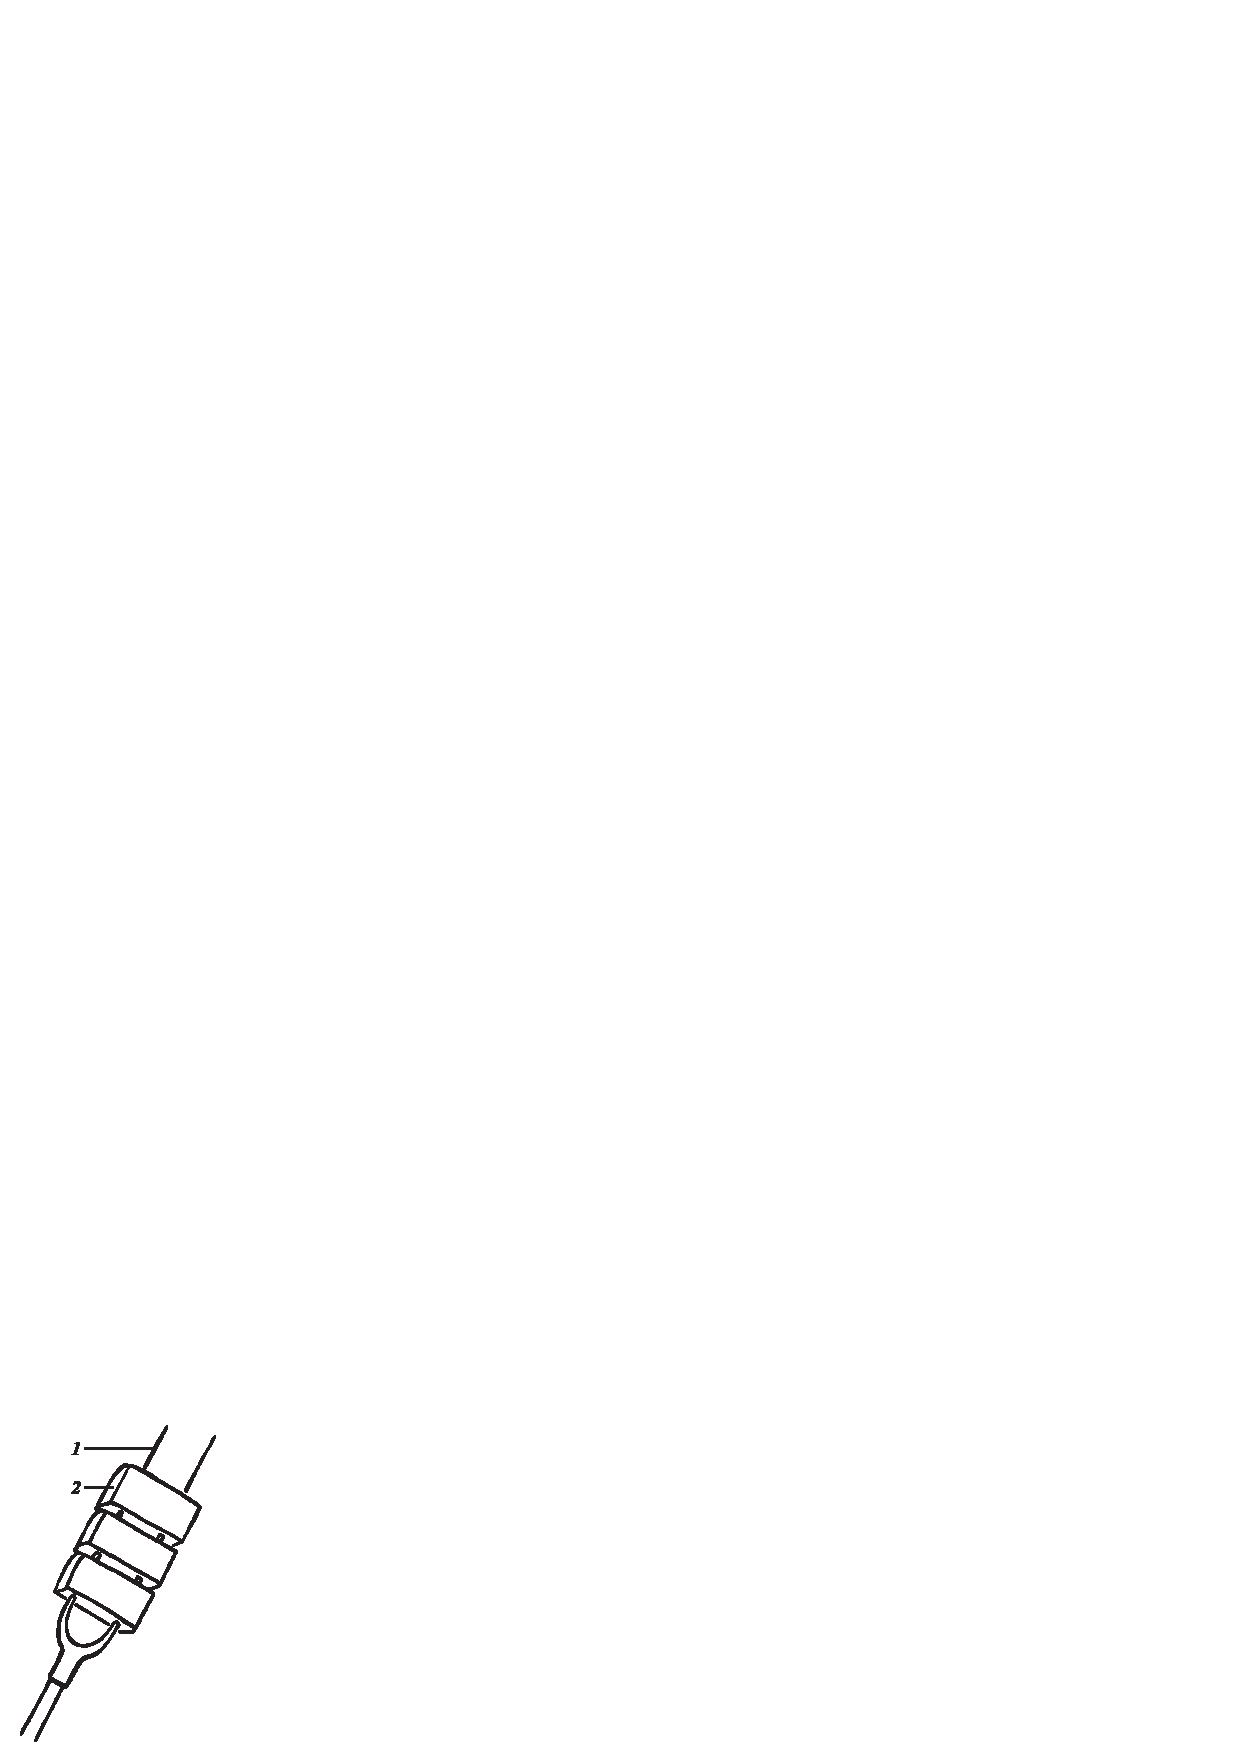
\includegraphics[scale=1]{illustration-011.pdf}%
\vspace{-.4375\baselineskip}%
\caption{叉烧宣腿叉法}
\label{叉烧宣腿}%
\begingroup%
\small%
\noindent%
\null\hspace{0em}1.铁叉\hspace{1em}2.火腿
\endgroup%
\end{wrapfigure}

\step 用刀将火腿均匀地切为三块,每块切成一寸三分宽、四寸半长,厚度为火腿本身的
厚度,用铁叉平叉起来(如图\,\ref{叉烧宣腿}\,)。将蛋清与豆粉调匀,涂于叉起来的
火腿上以保持原味,而免烧时走油走味。

\step 把杠炭三斤放入平炉上烧红,而后把叉好的火腿在平炉上以微火烘烤,要反复转动
叉柄,约二十分钟,烤至火腿熟透心时,揩净叉尖后取下叉子。用刀把火腿每隔两分远切
一刀,但不要完全切断,使其不会分开。然后摆在盘中,下面摆两块、上面摆一块成为
“品”字形。与烤熟的面包(切为十二片)和蒸好的荷叶饼同时上席。

\features

此菜外酥内香,为下酒的好菜。

\end{recipe}

% vim: filetype=tex noautoindent nojoinspaces
% vim: fileencoding=utf-8 formatoptions+=m
% vim: textwidth=78 tabstop=4 shiftwidth=4 softtabstop=4

\begin{recipe}{炸溜田鸡腿}

\ingredients

\ingredient{田鸡}{十五个}
\ingredient{鸡蛋}{一个}
\ingredient{干豆粉}{二钱}
\ingredient{盐}{二分}
\ingredient{酱油}{二钱}
\ingredient{姜片}{一钱}
\ingredient{葱}{二钱}
\ingredient{泡海椒}{二根}
\ingredient{料酒}{二钱}
\ingredient{胡椒面}{一分}
\ingredient{化猪油}{四两}
\ingredient{水豆粉}{一钱}

\preparation

\step 将田鸡剐后洗净,取下后两腿备用。泡海椒、葱切成马耳形。

\step 蛋清、豆粉、盐调匀,将田鸡腿拌匀;豆油、姜片、马耳葱、泡海椒节、料酒、胡
椒面加水豆粉调成滋汁备用。

待油锅热后,将田鸡腿放入锅内浸炸,待油浸透后, 起锅去骨,又将田鸡腿放入锅内,
将滋汁加热汤少许倒于田 鸡腿上,搅匀起锅即成。

\features

鲜嫩,味美,席桌热碟之一。

\end{recipe}

% vim: filetype=tex noautoindent nojoinspaces
% vim: fileencoding=utf-8 formatoptions+=m
% vim: textwidth=78 tabstop=4 shiftwidth=4 softtabstop=4

\begin{recipe}{五彩土司}

\ingredients

\ingredient{土司}{一磅}
\ingredient{鲜鱼肉}{八两}
\ingredient{猪肥膘}{二两}
\ingredient{鸡蛋}{五个}
\ingredient{熟瘦火腿}{五钱}
\ingredient{水发木耳}{五钱}
\ingredient{花椒面}{二分}
\ingredient{豆粉}{三钱}
\ingredient{芝麻}{五钱}
\ingredient{绿色小菜}{一两}
\ingredient{香油}{五钱}
\ingredient{蕃茄酱}{五钱}
\ingredient{生菜}{三两}
\ingredient{白糖}{三钱}
\ingredient{醋}{三钱}
\ingredient{盐}{五分}
\ingredient{菜油}{二斤耗一两五}

\preparation

\step 鲜鱼剔骨,去皮,选净细刺后,与肥膘分别用刀背砸茸搅成“鱼糁”。摊蛋皮一
张,连同火腿、木耳、绿色小菜分别切成各种细末,连芝麻共成五种细末各分装一边。

\step 土司修去周围的皮后,切成二分厚的片,先在一面抹上一层“蛋清豆粉”再放上“鱼
糁”约三分厚抹平,再将五种细末一样样摊开在墩子上,分颜色用刀口刮成一字条形,顺
着贴在“糁”上约一分厚,用手按平不脱,自成五色,每片同样贴好,上笼蒸五分钟取出。

\step 锅内掺油在旺火上烧至七成火,将土司放入,贴细末一面向上,炸成金黄色,将油
泌尽,淋上香油扦起;再用刀改成五分宽、一寸二长的条子(切时按五色切开使每片都现
彩色),装在条盘的一端,另一端放生菜。走菜时随椒盐一碟同上。

\features

色分五彩,美观;味兼香、酥、脆、嫩,为席桌行菜之一。

\end{recipe}

% vim: filetype=tex noautoindent nojoinspaces
% vim: fileencoding=utf-8 formatoptions+=m
% vim: textwidth=78 tabstop=4 shiftwidth=4 softtabstop=4

\begin{recipe}{兰花土司}

\ingredients

\ingredient{土司}{一^旁}
\ingredient{肥瞟}{二两}
\ingredient{鸡蛋清}{四个}
\ingredient{捃肝}{四个}
\ingredient{鲜鱼}{八两}
\ingredient{盐}{四分}
\ingredient{味精}{二分}
\ingredient{干豆粉}{五钱}
\ingredient{香油}{五钱}
\ingredient{葱白}{一两}
\ingredient{料酒}{二钱}
\ingredient{白糖}{一钱}
\ingredient{菜油}{^一斤耗一两五}
\ingredient{鉗酱}{三钱}

\cooking

土司切成三分厚片子〈共四片〉,鲜鱼打成“鱼糁”, 每个土司片上先抹蛋清豆粉,再涂上鱼糁,用手抹平整。

\step 腊肝四个去掉两面皮子4每个割为六个鸡冠花的形式 (共二十四个〉,用盐、料酒少许,抹匀后分别插在土司上 (每片六个分两边插〉,上笼蒸五分钟取出晾冷,每片土司 再开为六片待用。

菜油在旺火上烧至七成火候,将土司倒入锅内炸至浅 黄色,将油泌去,淋上香油,簸匀起锅入盘。

\step 白糖、香油、葱白、甜酱,兑成葱酱,镶入盘另一端 入席。

\notes

美观,酥脆,席桌行菜,下酒最宜。

\end{recipe}

% vim: filetype=tex noautoindent
% vim: fileencoding=utf-8
% vim: textwidth=78 tabstop=4 shiftwidth=4 softtabstop=4

\begin{recipe}{}

\ingredients

\ingredient{}{}

\cooking

\step

\notes

\end{recipe}

% vim: filetype=tex noautoindent
% vim: fileencoding=utf-8
% vim: textwidth=78 tabstop=4 shiftwidth=4 softtabstop=4

\begin{recipe}{酿冬截}

\ingredients

\ingredient{千冬菇}{三两}
\ingredient{盐}{一钱}
\ingredient{熟火腿}{六钱}
\ingredient{鸡蛋清}{四个}
\ingredient{黄秧白菜心}{一两}
\ingredient{葱白}{二钱}
\ingredient{干豆粉}{一两}
\ingredient{酱油}{四钱五}
\ingredient{姜}{二钱}
\ingredient{鸡脯肉}{二两五}
\ingredient{水豆粉}{六钱}
\ingredient{化猪油}{二两}
\ingredient{胡椒面}{二分五}
\ingredient{鸡油}{六钱}
\ingredient{猪肥礤肉}{一’两五}
\ingredient{味精}{三分}
\ingredient{鸡汤}{四两}
\ingredient{料酒}{一两}
\ingredient{冬笋(净)}{一两}

\cooking

\step 	干冬菇选菌盖直径约八分,大小均匀的二十四朵,用 清水一大碗泡半小时,至泡胀而未全胀时泌去水〈另作他 用)。换清水用手指在冬菇周围凸凹不平地方掏去泥沙,淘 洗干净,用刀齐盖底切去茎〔作别用);然后放在沸水中煮 约十分钟,端离火口浸泡十分钟捞出;再换清水烧沸同样再 煮一次,泌去煮水不用。此时菌盖直径已发胀至一寸二分左 右,则已干净胀透。

猪油倒入炒锅内,在旺火上烧至五成热,将葱白段、姜 (去皮、拍松)、盐、料酒、鸡汤依次放入,再加入冬菇、味 精、胡椒面同烧五分钟,使冬菇入味,将汤泌去,把冬菇捞 入筲箕中,将水滤干后放盘中摊开,切去茎的一面,向上摆 好待用。

\step 	鸡脯肉去掉外面一层白膜,在菜墩上用刀背棰成茸,

边捶边用刀口刮去肉内白筋,捶至极细为止。猪肥膘肉用刀 剁成肉泥(肉泥如同油脂,但不能化油;热天为了避免在剁 时化油,可先将肥膘肉放在冰箱内冰冻后再用,因化油要影 响搅成糁)。大碗内放入清水,把鸡茸投入用竹筷顺着一定 方向搅打五分钟,要搅散搅匀;随后放入鸡蛋清继续用力同 样搅打十分钟;再加入盐、味精、料酒、水豆粉,同时加入 肥肉泥,用力搅打五分钟成稀糊状(用筷蘸一点滴在清水面 上不沉底),即成鸡糁。

鸡蛋清二个与干豆粉调匀成为蛋清豆粉,在盘中摆好的 每个冬菇上的凹处抹上一层,再用调羹舀着鸡糁填满,随用 调羹刮平。然后装入蒸笼内(有糁一面向上)上笼蒸五分 钟,熟后取出待用(临用时才取,以保持热度)。

\step 火腿、冬笋切成长一寸三、宽三分、厚半分的片。黄 秧白菜心切成一寸半大小的块。猪油放入炒锅内,在旺火上 烧至五成热,即放入切好的火腿、冬笋、黄秧白菜,用汤瓢 翻搅两下,再迅速加入料酒、盐、酱油、鸡汤、味精、胡椒 面等佐料,用汤瓢搅匀。同时把蒸熟的冬菇翻入盘内(要使 冬菇盖顶向上〕,即用水豆粉将汁勾芡,淋入鸡油,再把汁 全部淋于冬菇面上即成。

\notes

此菜冬菇细嫩松脆,菌香味特浓,鲜美可口。

\end{recipe}

% vim: filetype=tex noautoindent
% vim: fileencoding=utf-8
% vim: textwidth=78 tabstop=4 shiftwidth=4 softtabstop=4

\begin{recipe}{软炸口茉}

\ingredients

\ingredient{口茉}{二两五}
\ingredient{猪油}{一斤约耗三两}
\ingredient{鸡蛋清}{三个}
\ingredient{鸡汤}{五两}
\ingredient{盐}{六分}
\ingredient{干豆粉}{一两}
\ingredient{味精}{二分}
\ingredient{料酒}{六钱}
\ingredient{姜}{二钱}
\ingredient{胡椒面}{一分五}
\ingredient{葱}{二钱}
\ingredient{香油}{二钱}
\ingredient{蕃茄酱}{二两}
\ingredient{白糖}{少许}

\preparation

\step 口茉选用大小均匀的,用清水泡半小时泌去水作别用,再换清水淘洗去泥沙。洗净
后用沸水煮十分钟,而后再换水煮十分钟,发至胀透,即成水发口茉。鸡蛋清与豆粉调成
干湿适度的蛋清豆粉。

\step 猪油放入锅内,在旺火上烧至五成热,放入葱、姜稍煸,即依次加入鸡汤、口茉、
料酒、盐、味精、胡椒面等烧约八分钟,用汤瓢将口茉捞出,入筲箕内滤干水,放入蛋清
豆粉内拌匀,使每块口茉都能裹上一层。

\step 猪油放入锅内,于旺火上烧至五成热,将裹好蛋清豆粉的口茉逐个放入稍炸。若火
过旺即将锅端离火口,炸至口茉上的蛋清豆粉刚熟(看不见黄色仍是白的)即捞入盘中。
要边放边捞,以免炸糊。若有粘连,可用手掰开。再将锅在旺火上烧至八成热,将盘中炸
过的口茉全部倒入,约炸五分钟呈金黄色时泌去炸油,随即淋入香油,捞出盛入盘中。另
以四个小碟盛入蕃茄酱(蕃茄酱加香油、白糖、味精、盐各少许)蘸食。

\features

此菜口茉皮酥内嫩,清香可口。

另一制作法:不裹蛋清豆粉而用糁裹口茉,味更鲜嫩。如用糁,原料上须增加鸡肉二两
五或鱼肉半斤、肥膘肉四两,作打糁用。

\end{recipe}

% vim: filetype=tex noautoindent nojoinspaces
% vim: fileencoding=utf-8 formatoptions+=m
% vim: textwidth=78 tabstop=4 shiftwidth=4 softtabstop=4

\begin{recipe}{海味什景}

\ingredients

\ingredient{熟鸡肉}{一两五}
\ingredient{猪心子}{一两五}
\ingredient{猪舌}{一两五}
\ingredient{猪肚}{一两五}
\ingredient{环喉}{三根}
\ingredient{蹄筋}{三根}
\ingredient{冬笋}{一五}
\ingredient{脊髓}{一两五}
\ingredient{口蘑}{三钱}
\ingredient{水发海参}{二两}
\ingredient{水发鱿鱼}{二两}
\ingredient{𧎼蛀}{三钱}
\ingredient{熟火腿}{三钱}
\ingredient{金钩}{三钱}
\ingredient{菜心}{五两}
\ingredient{酱油}{四钱}
\ingredient{糖汁}{少许}
\ingredient{化猪油}{两}
\ingredient{胡椒}{一分}
\ingredient{料酒}{五钱}
\ingredient{盐}{五分}
\ingredient{水豆粉}{五钱}
\ingredient{花椒}{数颗}
\ingredient{鸡汤}{三斤}
\ingredient{姜、葱}{各少许}

\preparation

\step 先将海参、鱿鱼、火腿切成二寸长、五分宽的片。以上的原料除去𧎼蛀、金钩外切
成大一字形条。脊髓用沸水汆过。海参、鱿鱼同样用沸水分开汆过。菜心泹后用清水漂起
待用。

\step 𧎼蛀放在蒸碗内上笼大火蒸𤆵,将锅放在旺火上,放下猪油,再放入姜葱,爆出香
味后,倒入鸡汤、盐、糖汁、料酒、酱油、花椒、胡椒及以上用沸水汆过的原材料(除鱿
鱼、海参、脊髓、小菜外)小火烧𤆵。再将小菜泹𤆵后,在白油锅内煸过,起锅垫入走菜
盘内。再将烧𤆵后的一字条,捞入盘内放在小菜上边。鱿鱼、脊髓,放在烧一字条等原料
的原汁内,烧上味打入盘内放在一字条块上边。再放入海参于原汁内烧上味,勾入豆粉,
起锅淋入盘内,海参放在鱿鱼、脊髓上面上席。

\features

美观大方,味浓可口,适宜四季头菜。

\end{recipe}

% vim: filetype=tex noautoindent nojoinspaces
% vim: fileencoding=utf-8 formatoptions+=m
% vim: textwidth=78 tabstop=4 shiftwidth=4 softtabstop=4

\pagebreak
\begin{recipe}{生片菊花锅}

\ingredients

\ingredient{鄉鱼}{八两}
\ingredient{胡椒}{三分}
\ingredient{粉条}{二钱}
\ingredient{油炸花生米}{一两五}
\ingredient{生鸡脯肉}{三两}
\ingredient{盐}{三分}
\ingredient{豌豆尖}{三两}
\ingredient{油条}{三根}
\ingredient{奶汤}{二斤半}
\ingredient{香菜}{一两}

\ingredient{干粉}{五钱}
\ingredient{菜油}{^一'斤耗三两}
\ingredient{葱}{二钱}
\ingredient{白菜心}{三两}
\ingredient{鸡捃肝}{三个}
\ingredient{味精}{三分}
\ingredient{菠菜}{五两}
\ingredient{猪腰}{四两}
\ingredient{化猪油}{一两}
\ingredient{姜}{二钱}
\ingredient{粗撒子}{二把}
\ingredient{白菊花}{一朵}

\cooking

\step 	鲫鱼洗净,去鱗,去肠杂,去刺〈刺留用〉,用刀切成 二寸长、一分厚、宽同鱼身的薄片。鸡腊肝洗净,去表皮, 切成薄片。生鸡脯肉片为一寸长、八分宽的薄片。猪腰去筋 和腰臊,切成鸡脯大小的薄片(以上薄片,愈薄愈好〉。这 四种片称为“四生片”,分别摆于七寸盘中成风车形。

\step 	菜油一斤入锅烧红,投入粉条,炸成黄色;花生米去

皮;油条切成一寸长段;撒子捏散(临上席时再用油炸一次 以保持酥脆〉;分别放入七寸盘内,称为“四油酥”。

白菜心洗净,用手撕去筋;豌豆尖淘洗,只留嫩苞; 菠菜去老叶和茎根部分;香菜洗净;分别放于七寸盘中,称 为“四鲜菜”。

\step 	姜一钱去皮,切成细末;葱切成葱花;与胡椒、味精 共摆一碟,每样占碟的四分之一。另以小碟盛盐备用。

\step 	鲜菊花一大朵(最好为自色〉,用刀切去花蒂,抽出 花蕊,仍以菊花原形放入盘中。

\step 	锅置火上,放入猪油,加入姜(拍松〉、葱切成五分 长的短节,随即放入奶汤和鱼骨刺,烧沸,约五分钟捞去鱼 骨刺和姜、葱,把汤舀入铜锅内为鱼羹汤。

\step 	桌上放一粗磁深盘,盘内盛酒精,盘上加铜架,架上 放铜锅,吃时将酒精燃烧,锅内汤沸时先将菊花放下,次将 各类生肉、生菜分别于汤内烫熟吃(除生片、生菜外其余油 蘇忌下锅内〉。

\notes

此菜宜于秋季吃,生片、鲜菜汤味清鲜,佐酒下饭均 宜。菜内生片、鲜菜可按季节变动,但只能用四样。冬季改 用梅花,即名“梅花锅”。

\end{recipe}

% vim: filetype=tex noautoindent
% vim: fileencoding=utf-8
% vim: textwidth=78 tabstop=4 shiftwidth=4 softtabstop=4

\begin{recipe}{}

\ingredients

\ingredient{}{}

\cooking

\step

\notes

\end{recipe}

% vim: filetype=tex noautoindent
% vim: fileencoding=utf-8
% vim: textwidth=78 tabstop=4 shiftwidth=4 softtabstop=4

\begin{recipe}[酿龙凤翅]{酿两样}

\ingredients

\ingredient{子鸡翅膀}{八对}
\ingredient{生猪排骨}{十六节}
\ingredient{鲜笋}{四两}
\ingredient{熟火腿}{二两}
\ingredient{水发冬菇}{二两}
\ingredient{鲜菜}{三两}
\ingredient{冰糖}{五钱}
\ingredient{酱油}{一两}
\ingredient{料酒}{五钱}
\ingredient{咮精}{三分}
\ingredient{水豆粉}{三钱}
\ingredient{香油}{二钱}
\ingredient{化鸡油}{三钱}
\ingredient{盐}{三分}
\ingredient{姜}{三钱}
\ingredient{葱}{五钱}
\ingredient{清汤}{二斤}
\ingredient{化猪油}{二两}
\ingredient{生鸡、猪骨}{一斤}
\ingredient{胡椒面}{一分}

\cooking

\step 选好八对子鸡翅后,用清水洗净粗皮,夹净细毛,在锅内煮熟,用清水冰冷;再放
至墩子上,从弯处切断,两头不用只要第二节。又选大生猪排十六节,二寸五长,在汤锅
内煮熟待用。

\step 鲜夢煮熟后切成一寸五长的头粗丝。火腿、冬燕,切成同样的一字条,分开放在盘
内;再拙去鸡翅及猪排的杆子骨;用铁夹将火腿、鲜笋、冬菇各夹一丝入抽去杆子骨处,
即成龙凤翅(鸡翅为凤,猪排为龙),放入盘内待用。

\step 生鸡、猪骨,用清水洗净,除去血水,放入罐内;龙凤翅放于罐内生鸡骨上面。

\step 炒锅放于旺火上,放下化油及糖,炒成糖汁,呈金黄色。再倒入清汤二斤,将糖汁
冲散,倒入盛龙凤翅的罐内,加入酱油、料酒、盐、老姜(拍破)、葱〔捆成把〕;将罐
在小火上烧四十分钟左右(汤烧至一半以上),龙凤翅已把,提离火口,捞起龙凤翅于二
鱼碗内,龙凤各占碗的一半。罐内的汤灌入二鱼碗内(留一半待用〕,放入笼内大火蒸三
十分钟待用。

\step 鲜菜洗净后炒熟放于碗内,再放化油于锅内,倒入罐内余的一半原汁、一分胡椒、
三分味精,水豆粉勾芡,再取出笼内的装龙凤翅的碗,将生菜放在碗的上边,再翻入大圆
盘内,淋入三钱化鸡油,余下的鸡油及香油二钱一并投入锅内,起锅将原汁淋于龙凤翅上
即成。

\features

味浓粑香,色美,四季可口,席桌走行菜。

\end{recipe}

% vim: filetype=tex noautoindent
% vim: fileencoding=utf-8 formatoptions+=m
% vim: textwidth=78 tabstop=4 shiftwidth=4 softtabstop=4

\end{tocminipageright}

\addtocounter{chapter}{2000}%
\addtocontents{toc}{\protect\enlargethispage{.5\baselineskip}}%
\category{重庆市部分菜肴}
\setlength{\cookbookafterrecipeskip}{.6875\baselineskip plus 1.1875\baselineskip}%

\begin{tocminipageleft}
\begingroup
\raggedbottom
\vspace{.25\baselineskip}
\begin{recipe}{}

\ingredients

\ingredient{}{}

\cooking

\step

\notes

\end{recipe}

% vim: filetype=tex noautoindent
% vim: fileencoding=utf-8
% vim: textwidth=78 tabstop=4 shiftwidth=4 softtabstop=4

\endgroup
\begin{recipe}{烟熏排骨}

\ingredients

\ingredient{猪签子排骨(正肋条)}{二斤}
\ingredient{小磨麻油}{二钱}
\ingredient{葱(切寸长小节V}{二根}
\ingredient{生姜(拍碎)}{三钱}
\ingredient{食盐}{一两}
\ingredient{柏枝}{五两}

\preparation

除去排骨边尖不整齐部分,以三根肋骨为一组宰成长方形块子。两面均匀地抹上细盐,将
姜、葱置排骨上盛在大碗内,上蒸笼蒸约半小时,到刚熟时取出,放入沸热卤水(一般卤
菜的卤水)中煮到熟软的程度,即肉与骨稍用力便可使之分离的时候取出。吃时油煎,热
置文火上炸之,炸到油冒出青烟即行取出,以鲜柏树枝烧烟熏约数分钟,刷上麻油,砍成
骨牌大小的块子即成。

\features

鲜嫩,清香爽口。

\end{recipe}

% vim: filetype=tex noautoindent
% vim: fileencoding=utf-8 formatoptions+=m
% vim: textwidth=78 tabstop=4 shiftwidth=4 softtabstop=4

\begin{recipe}{}

\ingredients

\ingredient{}{}

\cooking

\step

\notes

\end{recipe}

% vim: filetype=tex noautoindent
% vim: fileencoding=utf-8
% vim: textwidth=78 tabstop=4 shiftwidth=4 softtabstop=4

\begin{recipe}{冬菜蒸肉饼}

\ingredients

\ingredient{猪后腿瘦肉}{二两}
\ingredient{猪肥膘肉}{六钱}
\ingredient{阴米粉}{六钱}
\ingredient{冬菜}{四钱}
\ingredient{绍酒}{六钱}
\ingredient{黄豆芽(去根脚)}{六钱}
\ingredient{鸡蛋(搅散)}{一个}
\ingredient{食盐}{少许}
\ingredient{胡椒}{少许}
\ingredient{姜汁}{少许}

\cooking

肥、瘦肉均切成极细小的颗粒(不宜用刀宰,否则不散口〕,盛入碗内,加少许清水、阴
米粉、鸡蛋、绍酒、食盐、姜汁、胡椒等,混合搅掺,掺至水份为肉吸收时,制成圆饼状
,连同冬菜、豆芽盛入小磁盅内,加进清水(以水刚淹没肉饼为度),蒸约半小时即成。

\notes

细嫩散口,味道鲜美,营养丰富。

\end{recipe}

% vim: filetype=tex noautoindent
% vim: fileencoding=utf-8 formatoptions+=m
% vim: textwidth=78 tabstop=4 shiftwidth=4 softtabstop=4

\begin{recipe}{清汤竹荪肝膏}

\ingredients

\ingredient{竹荪}{二钱}
\ingredient{瘦猪肉}{二两五}
\ingredient{鸡脯肉}{四两}
\ingredient{母鸡汤}{六杓}
\ingredient{鸡蛋(取白)}{二个}
\ingredient{绍酒}{六钱}
\ingredient{食盐}{少许}
\ingredient{胡椒}{少许}

\preparation

竹荪以淘米水发胀后,轻轻搓几下漂入清水内。

鸡肝洗净以刀背捶绒,将蛋白搅散掺入鸡肝内,并加入胡椒、食盐和鸡汤一杓,合拌调匀。
以丝罗筛滤渣取汁,连续滤三次,然后将肝汁盛在碗内,蒸约十分钟即凝结成膏。蒸时火
力要适度,火大则会起蜂窝眼,火小则引起沉淀,不能凝结。

鸡汤五杓装在小铝锅内,在微火上烧沸,将浮油打起不要。将瘦猪肉用刀背捶绒,以冷汤
调散倾入鸡汤内,并加进绍酒用杓搅转,俟汤再沸时用漏杓将沉渣捞起不要。再将鸡脯肉
照样进行,并随时打净浮油,即成清汤(清汤时火力不宜大)。

临吃前将清汤轻轻转入肝膏碗里,并将发胀漂净的竹荪切成寸节放入,蒸熟即成。

\features

汤清彻如镜,味鲜美可口。竹荪乃本省特产。

\end{recipe}

% vim: filetype=tex noautoindent nojoinspaces
% vim: fileencoding=utf-8 formatoptions+=m
% vim: textwidth=78 tabstop=4 shiftwidth=4 softtabstop=4

\begin{recipe}{}

\ingredients

\ingredient{}{}

\cooking

\step

\notes

\end{recipe}

% vim: filetype=tex noautoindent
% vim: fileencoding=utf-8
% vim: textwidth=78 tabstop=4 shiftwidth=4 softtabstop=4

\begin{recipe}{锅贴肚头}

\ingredients

\ingredient{肚头}{二个}
\ingredient{荸荠}{四个}
\ingredient{绍酒}{少许}
\ingredient{味精}{少许}
\ingredient{鸡蛋(用白)}{一个}
\ingredient{姜}{数小片}
\ingredient{肥漆肉}{二两五}
\ingredient{熟火腿}{六钱}
\ingredient{胡椒、食盐}{少许}
\ingredient{千豆粉}{四钱}
\ingredient{葱}{数小节}
\ingredient{净冬笋}{六钱}

\preparation

肚头去筋皮,切成骨牌般大、铜元般厚的块子,与食盐、绍酒、胡椒、味精、姜葱等一齐
拌和均匀。肥膘肉煮熟后切成与肚头一样大的块子,将荸荠、冬笋、火腿切成小片,再将
蛋白与互粉泮成蛋清丑粉。

将肥膘肉抹干水气后,抹上蛋清豆粉。以荸荠、冬笋、火腿片摆在上面,又抹上蛋清豆粉,
再摆上一块肚头。锅烧辣后约下一汤瓢猪油,微烧后即倒去,留下少许猪油,移在小火上
煎炸上述片子。肚头朝上,肉片临锅,待肉煎成金黄色时,翻面将肚头那一面微煎,倒去
锅中所有的油,加进绍酒轻轻簸动,起锅即成。

\features

穌脆香美。

\end{recipe}

% vim: filetype=tex noautoindent nojoinspaces
% vim: fileencoding=utf-8 formatoptions+=m
% vim: textwidth=78 tabstop=4 shiftwidth=4 softtabstop=4

\end{tocminipageleft}
\begin{tocminipageright}
% BSD 3-Clause License
%
% Copyright (c) 2023 Quux System and Technology. All rights reserved.
%
% Redistribution and use in source and binary forms, with or without
% modification, are permitted provided that the following conditions are met:
%
% 1. Redistributions of source code must retain the above copyright notice, this
%    list of conditions and the following disclaimer.
%
% 2. Redistributions in binary form must reproduce the above copyright notice,
%    this list of conditions and the following disclaimer in the documentation
%    and/or other materials provided with the distribution.
%
% 3. Neither the name of the copyright holder nor the names of its
%    contributors may be used to endorse or promote products derived from
%    this software without specific prior written permission.
%
% THIS SOFTWARE IS PROVIDED BY THE COPYRIGHT HOLDERS AND CONTRIBUTORS "AS IS"
% AND ANY EXPRESS OR IMPLIED WARRANTIES, INCLUDING, BUT NOT LIMITED TO, THE
% IMPLIED WARRANTIES OF MERCHANTABILITY AND FITNESS FOR A PARTICULAR PURPOSE ARE
% DISCLAIMED. IN NO EVENT SHALL THE COPYRIGHT HOLDER OR CONTRIBUTORS BE LIABLE
% FOR ANY DIRECT, INDIRECT, INCIDENTAL, SPECIAL, EXEMPLARY, OR CONSEQUENTIAL
% DAMAGES (INCLUDING, BUT NOT LIMITED TO, PROCUREMENT OF SUBSTITUTE GOODS OR
% SERVICES; LOSS OF USE, DATA, OR PROFITS; OR BUSINESS INTERRUPTION) HOWEVER
% CAUSED AND ON ANY THEORY OF LIABILITY, WHETHER IN CONTRACT, STRICT LIABILITY,
% OR TORT (INCLUDING NEGLIGENCE OR OTHERWISE) ARISING IN ANY WAY OUT OF THE USE
% OF THIS SOFTWARE, EVEN IF ADVISED OF THE POSSIBILITY OF SUCH DAMAGE.
%
\begin{recipe}{干烧岩鲤}

\ingredients

\ingredient{岩鲤}{(二斤左右)一尾}
\ingredient{猪肥膘(切成小指头般大的颗粒)}{一两}
\ingredient{黄葱(切颗)}{六钱}
\ingredient{生姜米}{少许}
\ingredient{猪油}{二两五}
\ingredient{醋}{少许}
\ingredient{绍酒}{一两二}
\ingredient{味精}{少许}
\ingredient{豆瓣}{一两二}
\ingredient{蒜米}{少许}
\ingredient{酱油}{六钱}
\ingredient{白糖}{少许}
\ingredient{醪糟汁}{六钱}
\ingredient{肉汤}{二勺}

\preparation

鱼杀后去甲、鳃和内脏,洗净,在鱼的两侧肉上用刀斜划约两颗米深的刀线,每线距离约
一寸。在滚油锅里炸约一分钟,再用猪油在烧红的锅内煎辣,倾入豆瓣炒酥,即掺进肉汤,
稍煮后捞起豆瓣渣不要,及时放进鱼,倾入肥膘、蒜米、姜米、绍酒、醪糟汁、酱油、白
糖等,置文火上烧好为止(约半小时)。起锅时先将鱼取出盛入盘内,再将葱颗、味精、
醋等放进汤汁里,移在武火上,烧片刻以收干水份,使汤汁浓稠,淋在鱼上即成。

\features

肉细嫩、味鲜美,色泽光亮美观。此鱼系重庆市名产。

\end{recipe}

% vim: filetype=tex noautoindent nojoinspaces
% vim: fileencoding=utf-8 formatoptions+=m
% vim: textwidth=78 tabstop=4 shiftwidth=4 softtabstop=4

\begin{recipe}{}

\ingredients

\ingredient{}{}

\cooking

\step

\notes

\end{recipe}

% vim: filetype=tex noautoindent
% vim: fileencoding=utf-8
% vim: textwidth=78 tabstop=4 shiftwidth=4 softtabstop=4

\begin{recipe}{锅贴鱼}

\ingredients

\ingredient{乌鱼}{一斤}
\ingredient{鸡蛋(用蛋白)}{三个}
\ingredient{肥淥肉}{一斤半}
\ingredient{干豆粉}{一两}
\ingredient{净火腿}{一两}
\ingredient{食盐}{少许}
\ingredient{荸荠}{二两}

\preparation

肥膘肉煮熟,片成约一分厚、一寸半长的长方形块子;火腿、荸荠混合宰成碎末;蛋清与
豆粉调匀。用热帕抹干肉上的水气,涂上蛋清豆粉,把火腿、荸荠末涂在肉上。

将鱼剔去刺骨,同样片成块状薄片,在蛋清豆粉内拌过后,贴在肉上。

锅烧辣后下油,随即将上述肉块用文火煎熟,盛盘中,配以蕃茄酱、生菜或椒盐佐食。

\features

酥香、味美。

\end{recipe}

% vim: filetype=tex noautoindent nojoinspaces
% vim: fileencoding=utf-8 formatoptions+=m
% vim: textwidth=78 tabstop=4 shiftwidth=4 softtabstop=4

\begin{recipe}{}

\ingredients

\ingredient{}{}

\cooking

\step

\notes

\end{recipe}

% vim: filetype=tex noautoindent
% vim: fileencoding=utf-8
% vim: textwidth=78 tabstop=4 shiftwidth=4 softtabstop=4

\begin{recipe}{烟熏子鸡}

\ingredients

\ingredient{白皮肥嫩母鸡}{一只}
\ingredient{茶叶}{少许}
\ingredient{食盐}{一两}
\ingredient{红酱油}{三钱}
\ingredient{葱}{三根}
\ingredient{小磨麻油}{三钱}
\ingredient{生姜}{一块}
\ingredient{花株}{约二十颗}
\ingredient{耢糟水}{六钱}

\preparation

鸡去头脚,洗干净,晾干水气,里外均匀地抹上食盐,

胸部因肉厚要适当多抹。隔约半天,把姜拍碎,葱子打成小结子,连同花椒放在鸡腹内,
鸡的皮面以耢糟水抹上,用碗盛起,上笼蒸约二小时,蒸到软和时为度。在蒸的过程中,
每隔二三十分钟须刷麻油一次。鸡蒸好,取出时将红酱油刷在皮面上,使颜色美观,然后
用鲜柏树枝和少许茶叶燃起的烟子熏约半小时去掉腹内的姜、葱、花椒等,砍成约八分长
的斜方形小块,按鸡形盛于盘内即成。

\features

色泽金黄,味清香,鲜嫩。

\end{recipe}

% vim: filetype=tex noautoindent
% vim: fileencoding=utf-8 formatoptions+=m
% vim: textwidth=78 tabstop=4 shiftwidth=4 softtabstop=4

\begin{recipe}{椒麻鸡}

\ingredients

\ingredient{嫩公鸡(约重二斤)}{}
\ingredient{一只}{}

\ingredient{花椒}{约四十粒}
\ingredient{青葱}{一两}

\ingredient{生姜}{少许}
\ingredient{食盐}{二钱}
\ingredient{小磨麻油}{三钱}
\ingredient{白酱油}{一两二}
\ingredient{好醋}{三钱}

\cooking

将花椒、青葱生姜和倉盐等混合宰绒,宰时要适时淋 几滴小磨麻油。宰绒后盛入碗内加进小磨麻油、酱油、醋和 少许鲜汤,调成椒麻汁子。

鸡杀后去内脏洗净,用清水煮至八成熟时捞起,置冷开 水内浸冷后,连骨砍成一字条〈中指宽、一寸多长),按鸡形 盛入盘内,淋上汁子即可供食(将鸡剔骨撕成丝子亦可)。

\notes

肉细嫩,味清淡可口,夏天食之最宜。

\end{recipe}

% vim: filetype=tex noautoindent
% vim: fileencoding=utf-8
% vim: textwidth=78 tabstop=4 shiftwidth=4 softtabstop=4

\begin{recipe}{}

\ingredients

\ingredient{}{}

\cooking

\step

\notes

\end{recipe}

% vim: filetype=tex noautoindent
% vim: fileencoding=utf-8
% vim: textwidth=78 tabstop=4 shiftwidth=4 softtabstop=4

\end{tocminipageright}
\tocclearpage
\begin{tocminipageleft}
\begin{recipe}{}

\ingredients

\ingredient{}{}

\cooking

\step

\notes

\end{recipe}

% vim: filetype=tex noautoindent
% vim: fileencoding=utf-8
% vim: textwidth=78 tabstop=4 shiftwidth=4 softtabstop=4

\begin{recipe}{}

\ingredients

\ingredient{}{}

\cooking

\step

\notes

\end{recipe}

% vim: filetype=tex noautoindent
% vim: fileencoding=utf-8
% vim: textwidth=78 tabstop=4 shiftwidth=4 softtabstop=4

\begin{recipe}{}

\ingredients

\ingredient{}{}

\cooking

\step

\notes

\end{recipe}

% vim: filetype=tex noautoindent
% vim: fileencoding=utf-8
% vim: textwidth=78 tabstop=4 shiftwidth=4 softtabstop=4

\begin{recipe}{}

\ingredients

\ingredient{}{}

\cooking

\step

\notes

\end{recipe}

% vim: filetype=tex noautoindent
% vim: fileencoding=utf-8
% vim: textwidth=78 tabstop=4 shiftwidth=4 softtabstop=4

\begin{recipe}{酿茄饼}

\ingredients

\ingredient{茄子}{一斤}
\ingredient{姜米、葱花}{少许}
\ingredient{月巴瘦猪肉}{三两}
\ingredient{鸡蛋}{三个}
\ingredient{胡椒}{少许}
\ingredient{干豆粉}{酌量}
\ingredient{猪油}{二两五}
\ingredient{食盐}{少许}

\preparation

茄子切成厚度约二分的圆饼,每个圆饼切成火夹连,猪肉宰绒,与姜米、葱花、胡椒、食
盐、水豆粉拌和均匀,灌入火夹连的中间,以蛋清豆粉、食盐调转,涂在火夹连封口处,
制成茄饼,油烧至五成热时,下饼炸成鸭黄色,表皮已脆即成。吃时蘸以椒盐。

\features

表皮香脆,内瓤细嫩。

\end{recipe}

% vim: filetype=tex noautoindent nojoinspaces
% vim: fileencoding=utf-8 formatoptions+=m
% vim: textwidth=78 tabstop=4 shiftwidth=4 softtabstop=4

\begin{recipe}{核桃泥}

\ingredients

\ingredient{包谷粉}{三两七}
\ingredient{鸡蛋(黄白分开)}{三个}
\ingredient{瓜圆、桃米(宰成}{细颗)}
\ingredient{名—-两}{}
\ingredient{白糖}{三两七}
\ingredient{猪油}{三两七}

\cooking

包谷粉和以蛋黄加两杓清水调匀,猪油在锅里煎至约七八成火候,即倒进调好的包谷粉炒
熟,水份要炒干,要炒翻沙,炒熟后加进瓜圆、桃米和白糖,速即炒转,动作要快速,防
止巴锅。起锅时淋少许猪油,盛入盘中,同时将蛋白迅速掺泡,淋在上面。

\notes

香甜散口。

\end{recipe}

% vim: filetype=tex noautoindent
% vim: fileencoding=utf-8 formatoptions+=m
% vim: textwidth=78 tabstop=4 shiftwidth=4 softtabstop=4

\begin{recipe}{酿梨}

\ingredients

\ingredient{梨子}{四个}
\ingredient{糯米}{一两二}
\ingredient{蜜樱桃}{六钱}
\ingredient{瓜圆}{六钱}
\ingredient{百合、茨仁}{各三钱}
\ingredient{冰糖}{半斤}

\cooking

将梨子去皮,从蒂部揭盖将核挖去。糯米蒸熟,樱桃、瓜圆、百合切成小颗,与苡仁、糯
米一齐和转,灌入梨中,上笼蒸粑取下,同时将冰糖熬成糖水,浇淋梨上即成。

\features

香甜。

\end{recipe}

% vim: filetype=tex noautoindent
% vim: fileencoding=utf-8 formatoptions+=m
% vim: textwidth=78 tabstop=4 shiftwidth=4 softtabstop=4

\begin{recipe}{传丝杂烩汤}

\ingredients

\ingredient{洋菜}{一-两}
\ingredient{鸡蛋}{三个}
\ingredient{熟火腿(丝子)}{一两}
\ingredient{丝瓜(用皮切丝)}{一斤}
\ingredient{熟鸡丝}{一两}
\ingredient{酥肉(切成丝)}{二两}
\ingredient{熟猪肚(切丝)}{一两}
\ingredient{味精、胡椒面}{少许}
\ingredient{食盐}{酌量}
\ingredient{清汤(作法与清汤肝}{赏同)}
\ingredient{一大碗}{}

\preparation

洋菜用冷水发散,切成约二寸半长的节子。丝瓜皮切成约二寸半长的丝子,在开水中微煮
后捞起。鸡蛋调散烙成蛋皮,切成约二寸半长的丝子。将蛋皮丝、丝瓜丝、鸡丝、火腿丝
、酥肉丝、肚丝等用开汤透熟,岔开颜色摆在大碗中,上笼蒸熟后取下,将清汤加进味精
、食盐、胡椒等,烧开后灌入碗中即成。

\features

清淡鲜美,色泽美观。

\end{recipe}

% vim: filetype=tex noautoindent
% vim: fileencoding=utf-8 formatoptions+=m
% vim: textwidth=78 tabstop=4 shiftwidth=4 softtabstop=4

\begin{recipe}{清蒸肥头鱼}

\ingredients

\ingredient{肥头鱼(二斤左右)}{}
\ingredient{一尾}{}

\ingredient{火腿}{(切小片)一两}
\ingredient{网油}{六两}

\ingredient{胡:椒}{少许}
\ingredient{绍酒}{一两二}

\ingredient{食盐}{少许}
\ingredient{姜片}{六钱}
\ingredient{口蘑(发胀切片)}{几个}
\ingredient{黄葱}{二根}

\cooking

鱼杀后去内脏洗净,在两侧背肉上以刀斜划约二分深的 刀线,将口蘑和火腿片镶入刀线内,抹上食盐和胡椒,淋上 绍酒,以网油裹好盛入盘内,再加进姜片和黄葱蒸约半小时 即成(蒸时火要大)。临吃时蘸以姜米调醋(厨称毛姜醋

\notes

肥头鱼乃重庆市名产,肉质细嫩,味道鲜美。

\end{recipe}

% vim: filetype=tex noautoindent
% vim: fileencoding=utf-8
% vim: textwidth=78 tabstop=4 shiftwidth=4 softtabstop=4

\begin{recipe}{炒鸭脯}

\ingredients

\ingredient{肥鸭}{一只}
\ingredient{水豆粉}{少许}
\ingredient{食盐}{酌量}
\ingredient{蟮蛀}{二钱}
\ingredient{绍酒}{六钱}
\ingredient{火腿}{六钱}
\ingredient{鸡蛋(用白)}{四个}
\ingredient{荸荠}{―1麵1}
\ingredient{胡概面、味精}{少许}
\ingredient{猪油}{二两五}

\cooking

鸭杀后去头、脚、内脏,清洗干净,置笼上蒸圯取下,在背脊上开一长口(不伤背),小
心地剥下全身鸭皮,切成骨牌般大的块子,有条理地摆在碗中(皮背靠碗底),鸭皮须保
持滋润,勿使干燥。

剔下鸭脯肉连同鳐蛀、火腿、荸荠宰碎,盛在碗内,打下蛋清,加进味精、水豆粉、胡椒
面、食盐、绍酒及一杓鸡汤,调拌均匀。在锅中将猪油煎辣后,放下鸭脯炒四、五分钟,
铲在鸭皮上,上笼蒸约一分钟,取出翻在盘子上即成。

\features

肉质细嫩,味允鲜美。

\end{recipe}

% vim: filetype=tex noautoindent
% vim: fileencoding=utf-8 formatoptions+=m
% vim: textwidth=78 tabstop=4 shiftwidth=4 softtabstop=4

\begin{recipe}{}

\ingredients

\ingredient{}{}

\cooking

\step

\notes

\end{recipe}

% vim: filetype=tex noautoindent
% vim: fileencoding=utf-8
% vim: textwidth=78 tabstop=4 shiftwidth=4 softtabstop=4

\begin{recipe}{}

\ingredients

\ingredient{}{}

\cooking

\step

\notes

\end{recipe}

% vim: filetype=tex noautoindent
% vim: fileencoding=utf-8
% vim: textwidth=78 tabstop=4 shiftwidth=4 softtabstop=4

\begin{recipe}{}

\ingredients

\ingredient{}{}

\cooking

\step

\notes

\end{recipe}

% vim: filetype=tex noautoindent
% vim: fileencoding=utf-8
% vim: textwidth=78 tabstop=4 shiftwidth=4 softtabstop=4

\begin{recipe}{奶汤素烩}

\ingredients

\ingredient{窝笋头、胡萝卜、白萝卜}{各二两五}
\ingredient{净冬笋}{二两}
\ingredient{洋字}{四两}
\ingredient{(:以上各菜均切成约一指半宽的片子,并刻成各式花形)}{}
\ingredient{窝笋尖(去边叶乂}{五两}
\ingredient{瓢儿白(取心)}{五两}
\ingredient{黄秧白(取心),}{五两}
\ingredient{黄化}{数根}
\ingredient{冬菇(发胀)}{数片}
\ingredient{胡椒}{少许}
\ingredient{鸡汤}{四杓}
\ingredient{食盐}{少许}
\ingredient{鲜牛奶}{二两}
\ingredient{绍酒}{一两二}

\cooking

各种蔬菜分别煮至半熟,用清水漂冷,连同冬菇、黄花岔开颜色摆入盘内。鸡汤烧沸,轻
轻梭进摆好的各种蔬菜,加进胡椒、食盐和绍酒等,以文火烧至刚好时,即倒进牛奶,刚
煮沸后,起锅斜梭盘内,须保持原状不乱。

\notes

清淡可口,色泽美观,营养丰富。

\end{recipe}

% vim: filetype=tex noautoindent
% vim: fileencoding=utf-8 formatoptions+=m
% vim: textwidth=78 tabstop=4 shiftwidth=4 softtabstop=4

\begin{recipe}{网油黄秧白}

\ingredients

\ingredient{黄秧白}{八斤}
\ingredient{网油}{一斤半}
\ingredient{净火腿肉(切成寸长薄片)}{二两}
\ingredient{口蘑(发胀洗净切成小瓣)}{三钱}
\ingredient{豆粉}{一两}
\ingredient{绍酒}{二两五}
\ingredient{鸡汤}{三柏}
\ingredient{生鸡油}{六钱}
\ingredient{胡椒、味精}{少许}
\ingredient{鸡蛋(取白)}{二个}
\ingredient{冰糖色}{少许}
\ingredient{蟠蛀(洗净蒸熟)}{三钱}

\preparation

取黄秧白的心,洗净抽筋后,以沸水煮软捞起,晾干水气冷透。将网油去掉较厚部分,摊
伸铺上一层黄秧白菜,摆上火腿片、口蘑瓣和鳐蛀丝,再盖上一层黄秧白,即裹成茄子形
状(将以上材料裹成两只),以蛋清和豆粉调匀糊紧接口处,在滚油锅里微炸,捞起滤干
,放迸盛好鸡汤的锑锅里,同时放进绍酒、胡椒、冰糖色和鸡油等,以文火烧好为止(约
半小时)。起锅时取出鸡油渣放进味精,先将菜盛入盘内,再将汤汁移于大火上收浓淋上
即成。

\features

味浓厚鲜美,色泽美观。

\end{recipe}

% vim: filetype=tex noautoindent
% vim: fileencoding=utf-8 formatoptions+=m
% vim: textwidth=78 tabstop=4 shiftwidth=4 softtabstop=4

\begin{recipe}{干贝烧冬苋菜}

\ingredients

\ingredient{冬苋菜}{二斤}
\ingredient{干贞(蒸熟)}{三钱}
\ingredient{猪油}{一两}
\ingredient{绍酒}{六钱}
\ingredient{胡椒.}{少许}
\ingredient{食盐}{少许}
\ingredient{味情}{少许}
\ingredient{鸡汤}{五杓}

\preparation

冬苋菜洗干净,滴干水份。油煎辣后倾入冬苋菜,炒缩筋(厨称煸死),加进鸡汤二杓,
置于文火上烧至六成熟。同时以三杓鸡汤烧沸,加进味精、干贝、绍酒、食盐和胡椒,将
冬苋菜用漏杓捞起滤干转入汤内,再烧片刻。起锅时琳上少许水豆粉徙芡即成(菜不宜煮
得太烂,否则会失去原味

\features

清淡3味鲜,营养。

\end{recipe}

% vim: filetype=tex noautoindent nojoinspaces
% vim: fileencoding=utf-8 formatoptions+=m
% vim: textwidth=78 tabstop=4 shiftwidth=4 softtabstop=4

\begin{recipe}{豆渣烘猪头}

\ingredients

\ingredient{猪头肉}{一斤二两}
\ingredient{冰糖}{一两}
\ingredient{花椒}{十五粒}
\ingredient{大葱(切成小节)}{六钱}
\ingredient{小葱(切葱花)}{四钱}
\ingredient{豆渣}{七两}
\ingredient{绍酒}{一两}
\ingredient{老姜(拍破)}{四钱}
\ingredient{猪油}{二两五}
\ingredient{食盐}{酌量}

\cooking

将猪头的毛去尽,刮洗干净,在锅内煮到七分火色,以 刀切成寸多长的方形块子,置鏆或锑锅中,加清水约二中碗, 将冰糖炒化和绍酒、花椒、老姜、大葱、食盐一齐放下,用 武火烧开后,以文火烘约二小时半,到软如豆腐状时为止。 将肉放在碗内,放时有皮的一面向碗底,用漏瓢去掉汤内的 花椒、老姜、大葱等,把原汁淋在肉上,并放在蒸笼里去蒸。

将豆渣用清水淘洗干净,以筲箕滤干,用猪油在锅里烧 辣放入豆渣,炒干水气,到豆渣已酥,吐油成黄色时,将猪 头肉取出,并将其原汁倒进豆渣里,同时放进葱花、味精少 许及适当数量的食盐,稍炒后,盛入猪头肉上,然后翻盛盘 中供食。切忌久炒。吃时可以荷叶饼佐食。

\notes

肉质柔糯,肥而不腻,豆渣酥香。

\end{recipe}

% vim: filetype=tex noautoindent
% vim: fileencoding=utf-8
% vim: textwidth=78 tabstop=4 shiftwidth=4 softtabstop=4

\end{tocminipageleft}
\begin{tocminipageright}
\begin{recipe}{}

\ingredients

\ingredient{}{}

\cooking

\step

\notes

\end{recipe}

% vim: filetype=tex noautoindent
% vim: fileencoding=utf-8
% vim: textwidth=78 tabstop=4 shiftwidth=4 softtabstop=4

\begin{recipe}{椒盐蹄膀}

\ingredients

\ingredient{熟猪蹄膀}{一斤半}
\ingredient{水豆粉}{少许}

\preparation

将熟猪蹄膀晾干水气,在瘦肉部分抹上少许水豆粉,放入辣油锅内,炸到皮面酥脆时,打
起,油滴干后盛于盘中,以花卷、葱、酱、椒盐佐食。此系重庆一般作法,名为“软炸”。

另一炸法是:用三个鸡蛋与干豆粉调和均匀,涂在蹄膀上,下油锅中炸到微带黄红色。此
为酥炸,吃时仍以花卷、

葱、酱、椒盐佐食。

\features

酥脆香美,油而不腻。

\end{recipe}

% vim: filetype=tex noautoindent nojoinspaces
% vim: fileencoding=utf-8 formatoptions+=m
% vim: textwidth=78 tabstop=4 shiftwidth=4 softtabstop=4

\begin{recipe}{干煸牛肉丝}

\ingredients

\ingredient{瘦牛肉}{五两}
\ingredient{醪糟汁}{少许}
\ingredient{芹菜(切节子)}{三两}
\ingredient{菜油}{三两}
\ingredient{姜(切丝)}{少许}
\ingredient{食盐}{少许}
\ingredient{豆瓣}{三钱}
\ingredient{花椒面}{少许}
\ingredient{酱油}{少许}
\ingredient{蒜苗}{六钱}

\cooking

牛肉洗净切丝,油锅烧辣后,下牛肉、食盐、姜丝煸炒,牛肉将煸干时,下豆瓣,微煸后
,随下醪糟汁、芹菜、蒜苗、酱油,再行煸炒,待蒜苗煸熟即行起锅,撒上少许花椒面。

\notes

清香味美,肉质干而鲜嫩。

\end{recipe}

% vim: filetype=tex noautoindent
% vim: fileencoding=utf-8 formatoptions+=m
% vim: textwidth=78 tabstop=4 shiftwidth=4 softtabstop=4

% BSD 3-Clause License
%
% Copyright (c) 2023 Quux System and Technology. All rights reserved.
%
% Redistribution and use in source and binary forms, with or without
% modification, are permitted provided that the following conditions are met:
%
% 1. Redistributions of source code must retain the above copyright notice, this
%    list of conditions and the following disclaimer.
%
% 2. Redistributions in binary form must reproduce the above copyright notice,
%    this list of conditions and the following disclaimer in the documentation
%    and/or other materials provided with the distribution.
%
% 3. Neither the name of the copyright holder nor the names of its
%    contributors may be used to endorse or promote products derived from
%    this software without specific prior written permission.
%
% THIS SOFTWARE IS PROVIDED BY THE COPYRIGHT HOLDERS AND CONTRIBUTORS "AS IS"
% AND ANY EXPRESS OR IMPLIED WARRANTIES, INCLUDING, BUT NOT LIMITED TO, THE
% IMPLIED WARRANTIES OF MERCHANTABILITY AND FITNESS FOR A PARTICULAR PURPOSE ARE
% DISCLAIMED. IN NO EVENT SHALL THE COPYRIGHT HOLDER OR CONTRIBUTORS BE LIABLE
% FOR ANY DIRECT, INDIRECT, INCIDENTAL, SPECIAL, EXEMPLARY, OR CONSEQUENTIAL
% DAMAGES (INCLUDING, BUT NOT LIMITED TO, PROCUREMENT OF SUBSTITUTE GOODS OR
% SERVICES; LOSS OF USE, DATA, OR PROFITS; OR BUSINESS INTERRUPTION) HOWEVER
% CAUSED AND ON ANY THEORY OF LIABILITY, WHETHER IN CONTRACT, STRICT LIABILITY,
% OR TORT (INCLUDING NEGLIGENCE OR OTHERWISE) ARISING IN ANY WAY OUT OF THE USE
% OF THIS SOFTWARE, EVEN IF ADVISED OF THE POSSIBILITY OF SUCH DAMAGE.
%
\begin{recipe}{半汤鱼}

\ingredients

\ingredient{鲢鱼}{一斤}
\ingredient{猪油}{一两二}
\ingredient{白萝卜(切丝子)}{半斤}
\ingredient{食盐}{酌量}
\ingredient{姜片}{一钱}
\ingredient{胡椒面}{少许}
\ingredient{葱(切节子)}{一根}
\ingredient{味精、绍酒}{少许}

\preparation

将鱼片切成一分多厚的片子,用油微爆,即加进鸡汤二瓢半,并放下萝卜丝、姜、葱、食
盐、胡椒面,以大火煮三四分钟,起锅时稍加味精,吃时蘸以毛姜醋。

\features

味清淡,汤鲜美,可口。

\end{recipe}

% vim: filetype=tex noautoindent nojoinspaces
% vim: fileencoding=utf-8 formatoptions+=m
% vim: textwidth=78 tabstop=4 shiftwidth=4 softtabstop=4

\begin{recipe}{菜鱼汤}

\ingredients

\ingredient{鲜鱼块}{七两五}
\ingredient{鲜菜心}{酌量}
\ingredient{火腿}{几片}
\ingredient{鸡肉}{几片}
\ingredient{冬蒜}{几片}
\ingredient{葱}{几节}
\ingredient{味精}{少许}
\ingredient{豆瓣}{三钱}
\ingredient{酱油}{少许}
\ingredient{绍酒}{少许}
\ingredient{水豆粉}{少许}
\ingredient{猪油}{二两}

\preparation

鱼切成块子,微炸捞起。锅内留适量的油将豆瓣煵酥,加进汤约四瓢,滤去豆瓣渣,放下
鱼、菜心、火腿、鸡肉、冬菇、葱、酱油、绍酒,烧入味时,下味精及少许水豆粉即起锅。

\features

味鲜美,微辣。

\end{recipe}

% vim: filetype=tex noautoindent nojoinspaces
% vim: fileencoding=utf-8 formatoptions+=m
% vim: textwidth=78 tabstop=4 shiftwidth=4 softtabstop=4

\begin{recipe}{醋溜鸡}

\ingredients

\ingredient{去骨净嫩公鸡肉}{六两}
\ingredient{泡鉍海椒(切碎)}{六钱,}

\ingredient{莴笋头(切成指头般牡的梭子背形小块)}{二两}

\ingredient{蒜辨(切碎)}{一钱}
\ingredient{生姜(切碎)}{一钱}
\ingredient{猪油}{二两五}
\ingredient{黃葱(切颗粒状)}{三钱}
\ingredient{醋}{五钱}
\ingredient{酱油}{五钱}
\ingredient{白糖}{少许}
\ingredient{绍酒}{少许}
\ingredient{食盐}{酌量}
\ingredient{豆粉}{少许}

\cooking

将鸡肉用刀划若干条纹(如荔枝壳状〕后,切成大指头般厚的方块子,与绍酒、豆粉、食盐在碗内和拌,倾入辣油锅里快炒几铲,随即放进莴笋、泡海椒,再快炒二、三铲,同时将姜、葱、蒜、酱油、醋、白糖等在碗内调勻,迅即倾入锅内,继续快炒二、三铲,起锅即成。

\notes

味微酸,肉质细致。

\end{recipe}

% vim: filetype=tex noautoindent
% vim: fileencoding=utf-8 formatoptions+=m
% vim: textwidth=78 tabstop=4 shiftwidth=4 softtabstop=4

\begin{recipe}{}

\ingredients

\ingredient{}{}

\cooking

\step

\notes

\end{recipe}

% vim: filetype=tex noautoindent
% vim: fileencoding=utf-8
% vim: textwidth=78 tabstop=4 shiftwidth=4 softtabstop=4

\begin{recipe}{家常鸡}

\ingredients

\ingredient{净子公鸡肉}{七两}
\ingredient{泡海椒}{七钱}
\ingredient{净冬笋}{二两}
\ingredient{豆瓣辣酱}{六钱}
\ingredient{芹菜}{二两五}
\ingredient{酱油}{二钱五}
\ingredient{醋}{六分}
\ingredient{白糖}{六分}
\ingredient{水豆粉}{三钱五}
\ingredient{味精}{三分}
\ingredient{老姜米}{三分五}
\ingredient{绍酒}{三钱}
\ingredient{盐}{三分五}
\ingredient{清汤}{七钱}
\ingredient{猪油}{二两}

\preparation

将鸡肉和冬笋切成长一寸二分、宽二分的一字条,芹菜去头切成长一寸二分的段,泡海椒
剁碎。以水豆粉二钱、酱油五分及绍酒、盐同盛碗内,与鸡块拌和均匀。以醋、白糖、味
精、清汤及酱油二钱,水豆粉一钱半,同入碗中兑成汁子。锅烧热后,放下猪油,随下鸡
肉和冬笋,炒到水气将干

財5放入豆瓣、辣酱、姜,再稍炒后,即加进芹菜倾下已兑好的汁子,翻炒几下即可起锅。

\features

此菜极鲜嫩,带荔枝味。

\end{recipe}

% vim: filetype=tex noautoindent nojoinspaces
% vim: fileencoding=utf-8 formatoptions+=m
% vim: textwidth=78 tabstop=4 shiftwidth=4 softtabstop=4

% BSD 3-Clause License
%
% Copyright (c) 2023 Quux System and Technology. All rights reserved.
%
% Redistribution and use in source and binary forms, with or without
% modification, are permitted provided that the following conditions are met:
%
% 1. Redistributions of source code must retain the above copyright notice, this
%    list of conditions and the following disclaimer.
%
% 2. Redistributions in binary form must reproduce the above copyright notice,
%    this list of conditions and the following disclaimer in the documentation
%    and/or other materials provided with the distribution.
%
% 3. Neither the name of the copyright holder nor the names of its
%    contributors may be used to endorse or promote products derived from
%    this software without specific prior written permission.
%
% THIS SOFTWARE IS PROVIDED BY THE COPYRIGHT HOLDERS AND CONTRIBUTORS "AS IS"
% AND ANY EXPRESS OR IMPLIED WARRANTIES, INCLUDING, BUT NOT LIMITED TO, THE
% IMPLIED WARRANTIES OF MERCHANTABILITY AND FITNESS FOR A PARTICULAR PURPOSE ARE
% DISCLAIMED. IN NO EVENT SHALL THE COPYRIGHT HOLDER OR CONTRIBUTORS BE LIABLE
% FOR ANY DIRECT, INDIRECT, INCIDENTAL, SPECIAL, EXEMPLARY, OR CONSEQUENTIAL
% DAMAGES (INCLUDING, BUT NOT LIMITED TO, PROCUREMENT OF SUBSTITUTE GOODS OR
% SERVICES; LOSS OF USE, DATA, OR PROFITS; OR BUSINESS INTERRUPTION) HOWEVER
% CAUSED AND ON ANY THEORY OF LIABILITY, WHETHER IN CONTRACT, STRICT LIABILITY,
% OR TORT (INCLUDING NEGLIGENCE OR OTHERWISE) ARISING IN ANY WAY OUT OF THE USE
% OF THIS SOFTWARE, EVEN IF ADVISED OF THE POSSIBILITY OF SUCH DAMAGE.
%
\begin{recipe}{芙蓉鸡片}

\ingredients

\ingredient{母鸡脯肉}{二两五}
\ingredient{鸡蛋}{五个}
\ingredient{猪油}{一斤半}
\ingredient{火腿}{数片}
\ingredient{水豆粉}{少许}
\ingredient{豆尖}{一两}
\ingredient{冬笋}{数片}
\ingredient{姜片}{数片}
\ingredient{黄葱}{数节}
\ingredient{味精、食盐}{少许}
\ingredient{胡椒面}{少许}
\ingredient{冬菇}{数片}

\preparation

将鸡脯肉捶绒去筋、皮,盛入碗中,加进鸡汤调散,再加入蛋清、食盐、水豆粉拌和均
匀,不宜过稀过干。

锅烧辣后放下猪油,到油滚热现出小点子时,将上述鸡绒沿锅边倒下,这样鸡绒便浮在油
的上面,油烧开冲起来时,即将鸡绒连油一齐倒在大漏瓢内,滤去猪油。

将味精、食盐、胡椒面、水豆粉,连同少许鸡汤调和在一碗中。

在锅内用二两猪油烧辣,先下姜、葱,继下火腿、冬笋、冬菇、豆尖稍炒,随即倒下鸡
绒,以极迅速的手法炒数下,立即起锅。

\features

色泽纯白,泡如雪花,味道鲜美。

\end{recipe}

% vim: filetype=tex noautoindent nojoinspaces
% vim: fileencoding=utf-8 formatoptions+=m
% vim: textwidth=78 tabstop=4 shiftwidth=4 softtabstop=4

\begin{recipe}{}

\ingredients

\ingredient{}{}

\cooking

\step

\notes

\end{recipe}

% vim: filetype=tex noautoindent
% vim: fileencoding=utf-8
% vim: textwidth=78 tabstop=4 shiftwidth=4 softtabstop=4

\begin{recipe}{}

\ingredients

\ingredient{}{}

\cooking

\step

\notes

\end{recipe}

% vim: filetype=tex noautoindent
% vim: fileencoding=utf-8
% vim: textwidth=78 tabstop=4 shiftwidth=4 softtabstop=4

\begin{recipe}{小煎鸡}

\ingredients

\ingredient{嫩子公鸡(约二斤半重)}{一只}\
\ingredient{净冬笋}{二两}
\ingredient{芹黄}{一两}
\ingredient{泡海椒}{三个}
\ingredient{姜片}{数小片}
\ingredient{葱}{数节}
\ingredient{猪油}{二两}
\ingredient{酱油}{少许}
\ingredient{食盐}{少许}
\ingredient{白糖}{少许}
\ingredient{醋}{少许}
\ingredient{味精}{少许}

\cooking

鸡杀后去内脏洗净,剔去骨头,宰成约寸半长的筷子条,冬
笋也切成寸半长的筷子条,芹黄切成节子,泡海椒宰碎。将
鸡肉放在碗中,加入食盐及水豆粉拌和均匀。

猪油在锅内烧辣后放下鸡肉微炒,随即加进冬笋、泡海椒、
芹黄、姜、葱稍炒,同时将酱油、醋、白糖、味精、水豆粉
连同少许清汤在一碗内调成汁子,倾入锅中再炒几下,起锅
即成。

\notes

肉质细嫩,味清香鲜美。

\end{recipe}

% vim: filetype=tex noautoindent
% vim: fileencoding=utf-8
% vim: textwidth=78 tabstop=4 shiftwidth=4 softtabstop=4

% BSD 3-Clause License
%
% Copyright (c) 2023, 2024 Quux System and Technology. All rights reserved.
%
% Redistribution and use in source and binary forms, with or without
% modification, are permitted provided that the following conditions are met:
%
% 1. Redistributions of source code must retain the above copyright notice, this
%    list of conditions and the following disclaimer.
%
% 2. Redistributions in binary form must reproduce the above copyright notice,
%    this list of conditions and the following disclaimer in the documentation
%    and/or other materials provided with the distribution.
%
% 3. Neither the name of the copyright holder nor the names of its
%    contributors may be used to endorse or promote products derived from
%    this software without specific prior written permission.
%
% THIS SOFTWARE IS PROVIDED BY THE COPYRIGHT HOLDERS AND CONTRIBUTORS "AS IS"
% AND ANY EXPRESS OR IMPLIED WARRANTIES, INCLUDING, BUT NOT LIMITED TO, THE
% IMPLIED WARRANTIES OF MERCHANTABILITY AND FITNESS FOR A PARTICULAR PURPOSE ARE
% DISCLAIMED. IN NO EVENT SHALL THE COPYRIGHT HOLDER OR CONTRIBUTORS BE LIABLE
% FOR ANY DIRECT, INDIRECT, INCIDENTAL, SPECIAL, EXEMPLARY, OR CONSEQUENTIAL
% DAMAGES (INCLUDING, BUT NOT LIMITED TO, PROCUREMENT OF SUBSTITUTE GOODS OR
% SERVICES; LOSS OF USE, DATA, OR PROFITS; OR BUSINESS INTERRUPTION) HOWEVER
% CAUSED AND ON ANY THEORY OF LIABILITY, WHETHER IN CONTRACT, STRICT LIABILITY,
% OR TORT (INCLUDING NEGLIGENCE OR OTHERWISE) ARISING IN ANY WAY OUT OF THE USE
% OF THIS SOFTWARE, EVEN IF ADVISED OF THE POSSIBILITY OF SUCH DAMAGE.
%
\begin{recipe}{口袋豆腐}

\ingredients

\ingredient{嫩豆腐}{三块}
\ingredient{剔刺鱼肉}{一两八}
\ingredient{豆粉(碾细)}{六钱}
\ingredient{小苏打粉(碾细)}{少许}
\ingredient{鸡蛋(取白搅散)}{三个}
\ingredient{火腿(宰细)}{少许}
\ingredient{浓母鸡汤汁}{三勺}
\ingredient{绍酒}{三钱}
\ingredient{食盐}{少许}
\ingredient{胡椒}{少许}

\preparation

豆腐削去周围的表皮用刀背捣烂,挤干水份。以刀背将鱼肉捶绒,连同豆粉、苏打、食
盐、火腿和蛋清等加入豆腐内和拌均匀。用调羹连续盛入约七成滚的油内炸呈鸭黄色时捞
起,滤干,倾入烧沸的肉汤里汆一道,以去其油味,捞起再倾入浓鸡汤汁内,加入绍酒用
武火(不旺不小的火)煮约五分钟即成。起锅时才放进胡椒盛入碗内。

\features

味浓厚鲜美,富营养,内含浆包细嫩化渣,状似米口袋,故名“口袋豆腐”。

\end{recipe}

% vim: filetype=tex noautoindent nojoinspaces
% vim: fileencoding=utf-8 formatoptions+=m
% vim: textwidth=78 tabstop=4 shiftwidth=4 softtabstop=4

\begin{recipe}{清炖牛肉汤}

\ingredients

\ingredient{黄牛肉}{二十五斤}
\ingredient{老姜〈拍破)}{丰斤}
\ingredient{绍酒}{半斤}
\ingredient{味精}{二两五}
\ingredient{上等花椒}{一两六}
\ingredient{净鲜肥母鸡}{六斤}

\ingredient{食盆(炒后磨细)}{酌量}

\cooking

水牛肉质较粗,草气重,鲜味差,所以烛牛肉必须选用 黄牛肉,而黄牛肉适宜于清炖的又以后腿腿骨筋、千斤头、 肋占、筋管、前腿腿骨筋较好。不要用净瘦肉。

将挑选好的黄牛肉用冷水漂二十分钟,切成约重二斤半 的块子,放入特制的圆形白铁烛桶(高一尺三寸、直径七寸 五分)内。须分次放入,以便于分次除去泡沫。第一次放进 十五斤,同时下入沸水二十斤,在旺火上烧开后,撇去泡沫, 并约隔半小时从桶底翻动牛肉,以免粘锅。随即将其余十斤 半牛肉放下,俟烧开,又打去泡沫,加进老姜、花椒、绍酒、 母鸡(去头及爪),再行烧开,打去泡沫,然后移微火上炖着。

炖桶移在微火上后,应经常保持使汤微开的火力。肉炖 到五成熟时,将上下面的肉相互移位,使接受热力均勻。到 七成熟时,取出牛肉按纤维横切成一寸长、食指祖的一字 条,拣去不合格的皮筋,并按炤硬不同的程度分成三类,分 装三个炖桶中。同时,用干净稀白布滤去汤中老姜、花椒,也将 汤分盛入三个炖桶内,在旺火上烧开后,置微火上炖圯为止。 前后共需五小时半。母鸡只取其汁,炖好后取出作别用。

吃时可配以蔬菜,冬春天用萝卜,夏秋天用冬瓜或瓠子 瓜,切成一寸长、食指粗的一字条,另用锅煮熟,吃时加在 碗中,并酌加味精、食盐。

\notes

汤色清彻,汤味鲜香,肉质细嫩,油而不腻。

\end{recipe}

% vim: filetype=tex noautoindent
% vim: fileencoding=utf-8
% vim: textwidth=78 tabstop=4 shiftwidth=4 softtabstop=4

\begin{recipe}{清炖牛尾汤}

\ingredients

\ingredient{黄牛尾}{五斤}
\ingredient{老姜(拍破〉}{一'两五}

\ingredient{绍酒}{二两五}
\ingredient{味精}{一钱}
\ingredient{上等花椒}{六分}
\ingredient{猪油}{一两六}
\ingredient{净鲜肥母鸡}{三斤}
\ingredient{食盐(炒后磨细)}{七分半}

\cooking

将牛尾修去残余皮子,清洗干净。在每一骨节缝处切进 三分之二深,不切断,入清水内漂二十分钟。

用大锑锅盛开水六斤,放入牛尾,置旺火上烧开,打去 泡沫,继下老姜、花椒、绍酒、母鸡(去头及爪〉,再行烧 开后,移微火上炖,每隔一点多钟翻动一下,以免粘锅。炖 至七成熟时,以干净稀白布滤去汤中的花椒、老姜,重行放 在旺火上烧开后,又置微火上烛炤为止。前后共需炖七小时 半。母鸡只取其汁,烛好后,鸡取出作别用。吃时加味精 食盐和猪油。

\notes

汤浓鲜、香美,富营养。

\end{recipe}

% vim: filetype=tex noautoindent
% vim: fileencoding=utf-8
% vim: textwidth=78 tabstop=4 shiftwidth=4 softtabstop=4

\begin{recipe}{清炖枸杞牛鞭汤}

\ingredients

\ingredient{黄牛鞭}{二斤}
\ingredient{净鲜肥母鸡}{一斤}
\ingredient{绍酒}{一两五}
\ingredient{枸把}{二钱}
\ingredient{上等花椒}{二钱}
\ingredient{老姜(拍破)}{五线}
\ingredient{味精}{二钱}
\ingredient{猪油}{一两}


\ingredient{食盐(炒后磨细)}{五分}

\cooking

去尽牛鞭表皮,顺尿道对剖成两块。用清水洗干净,以 冷水漂三十分钟。

用锑锅盛开水六斤,放入牛鞭,置旺火上烧开,打去泡 沫,放下老姜、花椒、绍酒、母鸡,再行烧幵后移微火上炖。 每隔一点多钟翻动一下,以免粘锅。烛至六成熟时,以干净 稀白布滤去汤中的花椒、老姜,重置旺火上烧开后,移微火 上继续炖,炖到八成熟时,取出牛鞭,切成一寸长、食指祖 的一字条,仍放进锅内,同时放入枸杞,烧开后置微火上炖 钯为止。前后约共需炖十小时,鸡肉取出作别用。吃时加适 量味精、盐和猪油。

\notes

肉质糯嫩,汤浓味允,极富营养。

\end{recipe}

% vim: filetype=tex noautoindent
% vim: fileencoding=utf-8
% vim: textwidth=78 tabstop=4 shiftwidth=4 softtabstop=4

\vspace{1\baselineskip}
\begin{recipe}{炒牛肚梁}

\ingredients

\ingredient{净牛肚梁(切花)}{三两}
\ingredient{葱}{几小节}
\ingredient{泡海椒}{数小块}
\ingredient{食盐}{少许}
\ingredient{冬笋}{十余片}
\ingredient{酱油}{少许}
\ingredient{木耳}{少许}
\ingredient{菜淌}{一两玉-}
\ingredient{豆尖}{酌量}
\ingredient{水豆粉}{少许}
\ingredient{姜、蒜}{几小片}
\ingredient{白糖、绍酒}{少许}

\cooking

用食盐、水豆粉、绍酒与牛肚梁拌均匀,油烧辣后,下肚梁快速炒转,随下泡海椒、木
耳、冬笋、豆尖、姜、蒜、葱,再行炒转,同时用食盐、酱油、水豆粉、白糖及少许汤等
凋成汁子,迅即下锅,炒转即行起锅。

\notes

味浓香,富家常味。

\end{recipe}

% vim: filetype=tex noautoindent
% vim: fileencoding=utf-8 formatoptions+=m
% vim: textwidth=78 tabstop=4 shiftwidth=4 softtabstop=4

\end{tocminipageright}

\cleardoublepage

\appendix

\bookmarksetup{startatroot}%
\hypertarget{collation-notes}{}%
\bookmark[dest=collation-notes,level=section]{校勘记}%
% BSD 3-Clause License
%
% Copyright (c) 2023 Quux System and Technology. All rights reserved.
%
% Redistribution and use in source and binary forms, with or without
% modification, are permitted provided that the following conditions are met:
%
% 1. Redistributions of source code must retain the above copyright notice, this
%    list of conditions and the following disclaimer.
%
% 2. Redistributions in binary form must reproduce the above copyright notice,
%    this list of conditions and the following disclaimer in the documentation
%    and/or other materials provided with the distribution.
%
% 3. Neither the name of the copyright holder nor the names of its
%    contributors may be used to endorse or promote products derived from
%    this software without specific prior written permission.
%
% THIS SOFTWARE IS PROVIDED BY THE COPYRIGHT HOLDERS AND CONTRIBUTORS "AS IS"
% AND ANY EXPRESS OR IMPLIED WARRANTIES, INCLUDING, BUT NOT LIMITED TO, THE
% IMPLIED WARRANTIES OF MERCHANTABILITY AND FITNESS FOR A PARTICULAR PURPOSE ARE
% DISCLAIMED. IN NO EVENT SHALL THE COPYRIGHT HOLDER OR CONTRIBUTORS BE LIABLE
% FOR ANY DIRECT, INDIRECT, INCIDENTAL, SPECIAL, EXEMPLARY, OR CONSEQUENTIAL
% DAMAGES (INCLUDING, BUT NOT LIMITED TO, PROCUREMENT OF SUBSTITUTE GOODS OR
% SERVICES; LOSS OF USE, DATA, OR PROFITS; OR BUSINESS INTERRUPTION) HOWEVER
% CAUSED AND ON ANY THEORY OF LIABILITY, WHETHER IN CONTRACT, STRICT LIABILITY,
% OR TORT (INCLUDING NEGLIGENCE OR OTHERWISE) ARISING IN ANY WAY OUT OF THE USE
% OF THIS SOFTWARE, EVEN IF ADVISED OF THE POSSIBILITY OF SUCH DAMAGE.
%
\begingroup%
\vbadness=10000%
\small%
\begin{center}%
{%
	\Large\rmfamily\bfseries%
	\hbadness=10000\makebox[5em][s]{校勘记}%
}%
\end{center}%

\begin{list}{}{%
	\setlength{\topsep}{0pt}%
	\setlength{\leftmargin}{.529166mm}%
	\setlength{\rightmargin}{.529166mm}%
	\setlength{\listparindent}{\parindent}%
	\setlength{\itemindent}{\parindent}%
	\setlength{\parsep}{\parskip}%
	\addtolength{\textheight}{2.800042mm}%
}%
\item[]%

\vspace{0\baselineskip plus .5\baselineskip}%

本书原为成都市饮食公司所编纂。成都市饮食公司成立于一九五六年,是一家专营川菜、
成都小吃的特色餐饮企业。原书未公开出版,仅以内部资料发行于一九七二年七月。据编
印说明中记述,本书系参照《中国名菜谱第七辑》和《重庆名菜谱》修改整理而成。四川
省蔬菜水产饮食服务公司编纂,一九七七年七月发行的内部资料《四川菜谱》收集了两百
六十四个菜品,约有半数来自于本书。成都饮食公司一九八八年九月再版重印本书,仍以
内部资料发行。

今以《四川菜谱》成都市饮食公司一九七二年七月版为底本。校以《四川菜谱》成都市饮
食公司一九八八年九月版。《四川菜谱》四川省蔬菜水产饮食服务公司一九七七年七月
版、《中国名菜谱第七辑四川名菜点》商业部饮食服务业管理局一九六二年六月中国财政
经济出版社版,和《重庆名菜谱》重庆市饮食服务公司一九六〇年五月重庆人民出版社
版,亦尽可能采用。《四川菜谱》一九七二年七月版,省略称为《四》;《四川菜谱》一
九八八年九月版,省略称为《八》;《四川菜谱》四川省蔬菜水产饮食服务公司一九七七
年七月版,省略称为《七》;《中国名菜谱第七辑四川名菜点》,省略称为《中》;《重
庆名菜谱》,省略称为《重》。

校勘基本方针。保留异体字、方言用字。对已经弃用的同音简化字和类推简化字,恢复原
字。修正误植、错字、别字。

\vspace{1\baselineskip}%

二、七、八……全书各篇,“滗”。《四》本《八》本作“泌”。径改。“滗”,滤。

四、二四、七一……全书各篇,“搛”。《四》本《八》本作“扦”。径改。“搛”,(用筷子)
夹。

六、锅巴肉片。《四》本《八》本标题作“锅粑肉片”。据《中》本改。

七、水煮肉片。《四》本《八》本无脚注{\footnotesize\circled{1}}。据《中》本补。

八、一一、一六……全书各篇,“醪糟”,各本皆作“𰪿糟”。径改。“𰪿”系“𫃑”之类推简化
字。

九、芙蓉肉片。“使全部蘸裹在肉片上”。“蘸”,《四》本《八》本作“醮”。据《中》
本改。

一七、大南瓜蒸肉。各本皆作“掏尽内穰”。据《现代汉语词典》,“穰”今作“瓤”。

一八、一九,“尖刀圆子”。《四》本《八》本《七》本作“尖刀元子”。《中》本作“尖刀
丸子”。径改。

一八、二七九,“汆”。《四》本《八》本作“川”。径改。

一九、二〇、五六、一九五、二五四所附共十一副插图。《四》本《八》本插图,线条边
缘参差不齐模糊不清。据《中》本插图重制。

二二、三三,“肉圆”。《四》本《八》本作“肉元”。径改。

二四、四八、五五……全书各篇,“口蘑”。《四》本《八》本作“口茉”。据《中》本《重》
本改。

二八、二九、三三、一六三、二〇五、二〇六、二〇八、二五八、二七一,“圆”。《四》
本《八》本作“元”。径改。

二九、三十、三一、三二、九六、一七七、一七九、二六五、二六九、二九三、二九五、
三一〇、三一一,“铝锅”。各本皆作“锑锅”。径改。

三〇、芝麻肘子。“捡去泡沫”,《四》本《八》本作“检去泡沫”。径改。“杆杖”,《四》
本《八》本作“杆仗”。径改。

三三、三四、一四七、一八八、一九一,“圆子”。《四》本《八》本作“元子”。径改。

三七、炸扳指。“扳指”,《四》本《八》本作“斑指”,《中》本作“班指”。径改。
“……至肥肠起着皱折为适合。”“皱折”,《四》本作“绉折”。据《八》本改。

三九、四八、四九,“擀”。《四》本作“扞”。据《八》本改。

四〇、锅贴腰片。“磉磴”。
“磉”,{s\v{a}ng}{ㄙ\kern-.25emㄤ\kern-.75em\raise.5ex\hbox{\v{}}\kern.25em}
柱下石。
“磴”,{d\`{e}ng}{ㄉ\kern-.25emㄥ\kern-.75em\raise.5ex\hbox{\`{}}\kern.25em}
石阶。

四一、四二、七一、一二一、二五七,“𠟤”。疑误。

四一、二六五、二七〇,“臊”。《四》本《八》本作“骚”。径改。

四四、四九、八七、一〇六、一一七、二〇六、二四八,“烂”。《四》本《八》本作
“滥”。径改。

四八、菠饺白肺。“水龙头”,《四》本《八》本作“水笼头”。径改。

五〇、七九、八五……全书各篇,“蕃茄”。据《现代汉语词典》,今作“番茄”。

五二、六三、一四九、二五四,“劖”。《八》本作
“{\bfseries\raise.19em\hbox{\scalebox{.675}[.75]{免}}\kern-.675em%
\lower.215em\hbox{\scalebox{.95}[.55]{⺀}}\kern-.405616em%
\scalebox{.65}[1]{刂}}”,系已弃用之类推简化字。

五五、罈子肉。《八》本目录中作“罐子肉”。误。《中》本目录中作“坛子肉”,内页
中作“罎子肉”。

五五、六九、一五三,“须”。《四》本作“鬚”。据《八》本改。

五五、一八六、一八八……全书各篇,“珧柱”。《四》本《八》本作“𧎼蛀”。《中》本作
“𧎼柱”。径改。

五六、烤酥方。“将烤池内的红杠炭捡于烤池四周”。“捡”,《四》本《八》本《中》本皆
作“检”。径改。“在池中捡红杠炭一块”。“捡”,《四》本作“检”,《八》本作“拣”。据
《中》本改。

六三、辣子鸡丁。各本皆作“劖(音沾……)”。误。据《康熙字典》,“劖”,锄衔切,
读作{ch\'{a}n}{ㄔ\kern-.25emㄢ\kern-.75em\raise.5ex\hbox{\'{}}\kern.25em}。

六七、六八、八二、九二、一一八、一二七、一五〇、二五五、二八〇、三〇一,“熘”。
《四》本《八》本作“溜”。径改。

七一、贵州鸡。“搛入盘内”。“搛”,《八》本作“擀”。误。

七三、旱蒸全鸡。“箅子”,《四》本作“篦子”,《八》本作“篾子”。径改。

七四、三菌炖鸡。脚注{\footnotesize\circled{1}}中“……盛产于成都附近山崖中。”
《四》本《八》本作“……盛产于成都近郊。”据《中》本改。

八一、雪花鸡淖。“淖”,
{n\`{a}o}{ㄋ\kern-.25emㄠ\kern-.75em\raise.5ex\hbox{\`{}}\kern.25em} 泥也。

八七、牡丹鸡片。“擀”,《四》本作“扞”,《八》本作“撖”。径改。

九四、五彩鸡片。“㮟”,《八》本作“扞”。误。“㮟”,{k\={a}}{ㄎ\kern-.25emㄚ}
(紧)夹,扎,刺。

九五、刷把鸡丝。《八》本标题作“刷把鸡丝(汤)”。“上笼汽三分钟”。“汽”,《八》
本作“气”。误。

一〇〇、包烧鸡。“𫃕”,{c\'{i}}{ㄘ\kern-.75em\raise.5ex\hbox{\'{}}\kern.25em}
粘稠。

一〇一、包烧鸡。“鸡翘”,鸡屁股。

一〇二、魔芋烧鸭。“魔芋”,《四》本《八》本作“茉芋”。径改。

一〇六、银杏鸭脯。“锅内掺清汤”。“掺”,《四》本《八》本作“渗”。径改。

一二〇、一二一、一二三、二二三、二五七、二六二,“𬂁”。“肫”之异体字。鸟类的胃。

一二〇、一二九、一三〇……全书各篇,“鳃”。各本皆作“腮”。径改。

一二一、汆双脆。《四》本《八》本标题作“川双脆”。径改。

一四二、红烧甲鱼。“甲鱼”,《四》本《八》本全篇皆作“足鱼”。据《中》本《七》本
改。“肉𤆵可口”,《中》本作“肉烂可口”。“但须注意甲鱼肉不可与苋菜同食”。“甲鱼
肉”,《中》本作“龟鳖肉”。

一四三、黄焖大鲢鱼头。《四》本《八》本中脚注标记{\footnotesize\circled{1}}在
“原料”段落中“鲢鱼头一个约四、五斤”之后。据《中》本改至标题之后。“竹篾箅”,
《四》本《八》本作“竹篾篦”。据《中》本改。“即用筷子将鱼肉轻轻拨下”,《四》本
《八》本作“……轻轻试一下”。据《中》本改。脚注{\footnotesize\circled{1}}中“而不
是一般池塘养的鲢鱼”,《四》本《八》本无此句。据《中》本补。之后“但四川人……”,
《四》本《八》本无“但”字。据《中》本补。脚注{\footnotesize\circled{1}}中“身圆
口大”,《四》本《八》本作“身团口大”。据《中》本改。

一四四、五柳鱼。“酱油、白糖、醋、味精、水豆粉、料酒、清汤先兑成滋汁一碗。”“白
糖”,《八》本作“冰糖”。

一四七、一五〇,“鱼圆”。《四》本《八》本作“鱼元”。径改。

一四八、椒盐鱼卷。“咖喱”,《四》本《八》本作“咖哩”。径改。

一五七、一七三、一七八、一八二、一八三、一八四、一八五、一九三、二六三,“煨”。
《四》本《八》本作“喂”。径改。

一六三、五色虾球。“鲜虾仁”,《四》本《八》本“鲜”前衍一“尽”字。径删。

一六九、佛手蜇卷。“蜇”,《八》本作“蛰”。误。

一八三、菠饺鱼肚。“擀”,《四》本《八》本作“扞”。径改。

一九四、佛手海参。“白铝盘”,《四》本《八》本作“白锑盘”。径改。

二〇二、二〇四,“红苕”。亦称番薯、红薯、甘薯。

二〇四、蜜汁苕蛋。“青糖”,《四》本《八》本作“清糖”,径改。“青糖”,粗制赤(红)
糖。

二〇四、二〇七,“橘红”。《四》本《八》本作“桔红”。径改。

二〇五、糯米圆子。“圆子”,《四》本《八》本《中》本作“元子”。径改。“入沸水潦过
心”。“潦”,疑误。

二〇七、八宝酿藕。“百合”,《四》本《八》本作“白合”。径改。

二一二、盐白菜冬笋。“大拇指”,《四》本《八》本作“大姆指”。据《中》本改。

二二三、二六一,“什锦”。《四》本《八》本作“什景”。径改。

二二八、格花豆腐皮。“四张豆腐皮一叠,如果再重四张,共为两叠。”“叠”,《四》本
《八》本作“迭”。径改。

二三三、清汤白菜。《四》本“八分火”之后无脚注标记{\footnotesize\circled{1}}。据
《八》本《中》本补。

二四五、酸辣虾羹汤。“盐六分”,《四》本《八》本作“盐一分”。据《中》本改。《四》
本《八》本无脚注{\footnotesize\circled{1}\circled{2}\circled{3}\circled{4}}。
据《中》本补。

二五三、子母烩。《中》本标题作“子母会”。“因鸽子与鸽蛋同配一菜,故名子母会
(烩)。”《四》本《八》本括号部分在句号后面。《中》本无括号部分内容。据《标点
符号用法》\textsc{gb/t 15834--2011},将括号部分移至句号之前。

二六七、炸扳指。“扳指”,《四》本《八》本《重》本作“斑指”。径改。

二六七、三〇八,“汆一道”。《四》本《八》本作“川一道”。径改。

二六九、清汤竹荪肝膏。“竹荪”,《四》本《八》本《重》本皆作“竹参”。径改。

二七三、旱蒸鱼。各本标题皆作“汗蒸鱼”。径改。

二九二、奶汤素烩。“莴笋”,《四》本《八》本作“窝笋”。径改。

\end{list}
\endgroup%

% vim: filetype=tex noautoindent nojoinspaces
% vim: fileencoding=utf-8 formatoptions+=m
% vim: textwidth=78 tabstop=4 shiftwidth=4 softtabstop=4

\clearpage
\hypertarget{index}{}%
\bookmark[dest=index,level=section]{索引}%
\begingroup%
\small%
\printindex
\endgroup%
\cleardoublepage

\backmatter

\pagestyle{empty}
\pagenumbering{Alph}%   Upper case letter page numbers (and reset to 1)
\setcounter{page}{23}%  Letter W
\bookmarksetup{startatroot}%
\null%
\clearpage
\hypertarget{colophon}{}%
\bookmark[dest=colophon,level=section]{版次标记}%
% BSD 3-Clause License
%
% Copyright (c) 2023 Quux System and Technology. All rights reserved.
%
% Redistribution and use in source and binary forms, with or without
% modification, are permitted provided that the following conditions are met:
%
% 1. Redistributions of source code must retain the above copyright notice, this
%    list of conditions and the following disclaimer.
%
% 2. Redistributions in binary form must reproduce the above copyright notice,
%    this list of conditions and the following disclaimer in the documentation
%    and/or other materials provided with the distribution.
%
% 3. Neither the name of the copyright holder nor the names of its
%    contributors may be used to endorse or promote products derived from
%    this software without specific prior written permission.
%
% THIS SOFTWARE IS PROVIDED BY THE COPYRIGHT HOLDERS AND CONTRIBUTORS "AS IS"
% AND ANY EXPRESS OR IMPLIED WARRANTIES, INCLUDING, BUT NOT LIMITED TO, THE
% IMPLIED WARRANTIES OF MERCHANTABILITY AND FITNESS FOR A PARTICULAR PURPOSE ARE
% DISCLAIMED. IN NO EVENT SHALL THE COPYRIGHT HOLDER OR CONTRIBUTORS BE LIABLE
% FOR ANY DIRECT, INDIRECT, INCIDENTAL, SPECIAL, EXEMPLARY, OR CONSEQUENTIAL
% DAMAGES (INCLUDING, BUT NOT LIMITED TO, PROCUREMENT OF SUBSTITUTE GOODS OR
% SERVICES; LOSS OF USE, DATA, OR PROFITS; OR BUSINESS INTERRUPTION) HOWEVER
% CAUSED AND ON ANY THEORY OF LIABILITY, WHETHER IN CONTRACT, STRICT LIABILITY,
% OR TORT (INCLUDING NEGLIGENCE OR OTHERWISE) ARISING IN ANY WAY OUT OF THE USE
% OF THIS SOFTWARE, EVEN IF ADVISED OF THE POSSIBILITY OF SUCH DAMAGE.
%
\begingroup%

% XeLaTeX
\newcommand\XeLaTeX{%
	X\kern-.1em\lower.5ex\hbox{\scalebox{-1}[1]{E}}\kern-.15em%
	L\kern-.36em\raise.428571ex\hbox{\scalefont{.7}{A}}\kern-.15em%
	T\kern-.166667em\lower.5ex\hbox{E}\kern-.125em{X}%
}

\footnotesize%
\singlespacing%
\setlength{\parindent}{0pt}%
\setlength{\parskip}{.5\baselineskip}%

\null

\vfill

\begin{tabbing}
\hspace{9.5625em}\= \kill
\textsc{git} commit name:       \>\texttt{\gitcommitname}\\
\textsc{git} commit hash:       \>\texttt{\gitcommithash}\\
\textsc{git} committer date:    \>\texttt{\gitcommitterdate}\\
\textsc{pdf} build date:        \>\texttt{\pdfbuilddate}\\
\textsc{pdf} build host:        \>\texttt{\pdfbuildhost}
\end{tabbing}

This book is composed in \XeLaTeX.

\vspace{1\baselineskip}

\textsc{Quux} System and Technology

\endgroup%

% vim: filetype=tex noautoindent nojoinspaces spell spelllang=en
% vim: fileencoding=utf-8 formatoptions+=m
% vim: textwidth=78 tabstop=4 shiftwidth=4 softtabstop=4

\cleardoublepage

\hypertarget{inside-back-cover}{}%
\bookmark[dest=inside-back-cover,level=section]{封三}%
\null%
\clearpage

% Back cover
\hypertarget{back-cover}{}%
\bookmark[dest=back-cover,level=section]{封底}%
\includepdf[pages=1]{back-cover.pdf}

\end{cookbook}
\end{document}

% vim: filetype=tex noautoindent nojoinspaces
% vim: fileencoding=utf-8 formatoptions+=m
% vim: textwidth=78 tabstop=4 shiftwidth=4 softtabstop=4
